\documentclass[11pt]{book}

\usepackage{cdtUsecases}
\usepackage{txfonts}
\usepackage{mathptmx}         % Cambia la fuente a Times New Roman o equivalente
\usepackage[utf8]{inputenc}   % Permite caracteres especiales
\usepackage[T1]{fontenc}      % Mejora el manejo de caracteres (como acentos)
\usepackage{setspace}  
\usepackage{xcolor}
\usepackage{hyperref}  
\usepackage{caption}     % Controla el espaciado (opcional)
\bibliographystyle{ieeetr} % Estilo ieeetr


\captionsetup{font=small}

\hypersetup{
    colorlinks=true,    % Activa los enlaces coloreados
    citecolor=blue,     % Citas en azul
    linkcolor=blue,     % Enlaces internos (índices, TOC) en azul
    urlcolor=blue       % URLs en azul
}

\title{Entregable C2-EP2\bigskip\\Nombre del Proyecto}
\subtitle{Componente 2 Iteración 2 Especificación del proyecto}
\author{Nombre del equipo o consultoría}
\organization{Escuela Superior de Cómputo, IPN}
\showInstrucciones
\date{\color{red}Borrador del 21 de febrero del 2017\\(para revisión)}
%\date{\color{green}Version 1.0}

%%%%%%%%%%%%%%%%%%%%%%%%%%%%%%%%%%%%%%%%%%%%%%%%%%%%%%%%%%%%%%%%
\begin{document}

%\ThisLRCornerWallPaper{1}{theme/bannerAzul} 
\maketitle
\thispagestyle{empty}


\frontmatter
\tableofcontents
\listoffigures 
\listoftables

% 
%=========================================================
%\chapter{Project Charter}

\newcommand{\ESCOMPchSec}[1]{\rowcolor{colorAgua}\multicolumn{4}{|c|}{\bf #1}\\\hline}
\newcommand{\ESCOMPchItem}[2]{{\bf {#1}} & \multicolumn{3}{p{.66\textwidth}|}{#2}\\\hline}
\newcommand{\ESCOMPchSubItem}[3]{{\bf {#1}} & {#2} & \multicolumn{2}{p{.44\textwidth}|}{#3}\\\hline}
\newcommand{\ESCOMPchSubSubItem}[4]{{\bf {#1}} & {#2} & {#3}& {#4}\\\hline}

\cleardoublepage
{\centering{\Huge Project Charter}\bigskip\\}
\begin{table}[hptb!] 
%\renewcommand\thetable{i}
\begin{tabular}{|p{.22\textwidth} |p{.22\textwidth} |p{.22\textwidth} |p{.22\textwidth} |}
	\hline
	\ESCOMPchItem{Proyecto:}{CVE, Nombre proyecto.}
	\ESCOMPchItem{Responsable:}{Empresa, Nombre del responsable, cargo, Firma.}
	\ESCOMPchItem{Autoriza:}{Empresa, Nombre del responsable, cargo, Firma.}
	\ESCOMPchItem{Background/Contexto:}{Descripción breve del contexto, no mas de 3 líneas.}
	\ESCOMPchItem{Beneficios esperados:}{Principales beneficios al término del proyecto.}
	\ESCOMPchItem{Costo estimado:}{\$ 2,350,700.00 $\pm$ 13\% (por ejemplo.)}
	\ESCOMPchSubSubItem{Fecha de inicio:}{Fecha}{\bf Fecha de término:}{Fecha.}
	\ESCOMPchItem{Objetivo:}{Objetivo general del proyecto.}
	\ESCOMPchSec{Entregables Principales}
	\ESCOMPchSubItem{}{Clave-Nombre}{descripción del entregable}
	\ESCOMPchSubItem{}{Clave-Nombre}{descripción del entregable}
	\ESCOMPchSubItem{}{...}{}
	\ESCOMPchSec{Alcance del proyecto}
	\ESCOMPchItem{Incluye:}{
		\begin{Titemize}
			\Titem Elemento 1 del alcance que incluye.
			\Titem ...
		\end{Titemize}
	}
	\ESCOMPchItem{Excluye:}{
		\begin{Titemize}
			\Titem Elemento 1 del alcance que incluye.
			\Titem ...
		\end{Titemize}
	}
	\ESCOMPchItem{Criterio de éxito:}{Indicador clave de término del proyecto}
	\ESCOMPchItem{Metodología:}{Metodología o metodologías que se utilizan (dos renglones o lista de no mas de 7)}
	\ESCOMPchSec{Datos de contacto}
	\ESCOMPchItem{Project Manager:}{Nombre, Tel, correo, etc.}
	\ESCOMPchItem{Project owner:}{Nombre, Tel, correo, etc.}
	\ESCOMPchItem{...}{}
	\ESCOMPchItem{Riesgos y peligros:}{
		\begin{Titemize}
			\Titem Riesgo o peligro identificado.
			\Titem ...
		\end{Titemize}
	}
	\ESCOMPchItem{Supuestos:}{
		\begin{Titemize}
			\Titem Suposiciones hechas de las que depende el éxito del proyecto.
			\Titem ...
		\end{Titemize}
	}
	\ESCOMPchItem{Restricciones y dependencias:}{
		\begin{Titemize}
			\Titem Restricciones del proyecto.
			\Titem ...
		\end{Titemize}
	}
	\ESCOMPchSec{Supervisión}
	\ESCOMPchSubItem{Juntas:}{(Nombre de la(s) persona(s)),}{ reporta a (Nombre de la(s) persona(s))}
	\ESCOMPchSubItem{Dudas:}{(Nombre de la(s) persona(s)),}{ reporta a (Nombre de la(s) persona(s))}
	\ESCOMPchSubItem{Avances:}{(Nombre de la(s) persona(s)),}{ reporta a (Nombre de la(s) persona(s))}
	\ESCOMPchSubItem{...}{}{}
\end{tabular}
	\caption{Resumen del proyecto}
	\label{tbl:projectCharter}
\end{table}


\mainmatter 
%\LRCornerWallPaper{1}{theme/plecaAyD} 

%%%%%%%%%%%%%%%%%%%%%%%%%%%%%%%%%%%%%%%%%%%%%%%%%%t%%%%%%%%%%%%%%

%=========================================================
    %%=========================================================
\chapter{Introducción}


\cdtInstrucciones{
	Presentar el documento, indicando su contenido, a quien va dirigido, quien lo realizó, por que razón, dónde y cuando. \\
}
	Este documento contiene la Especificacion del ptoyecto ``{\em Nombre del proyecto}'' correspondiente al trabajo realizado en el semestre 2016-2017-2 para la materia de Análisis y diseño orientado a objetos en el grupo 2CV9 por el equipo {\em Nombre del equipo}.

%---------------------------------------------------------
\section{Presentación}


\cdtInstrucciones{
	Indique el propósito del documento y las distintas formas en que puede ser utilizado.\\
}
	Este documento contiene la especificación de los requerimientos del usuario y del sistema del sistema a desarrollar. Tiene como objetivo establecer la naturaleza y funciones del sistema para su evaluación al final del semestre. Este documento debe ser aprobado por los principales responsables del proyecto.
	
	Este documento es el C2-EP1 del proyecto ``{\em Nombre del proyecto}''.
	
%---------------------------------------------------------
\section{Organización del contenido}

	En el capítulo \ref{cap:reqUsr} ...
	
	En el capítulo \ref{cap:reqSist} ...

%---------------------------------------------------------
\section{Notación, símbolos y convenciones utilizadas}

	Los requerimientos funcionales utilizan una clave RFX, donde:
	
\begin{description}
	\item[X] Es un número consecutivo: 1, 2, 3, ...
	\item[RF] Es la clave para todos los {\bf R}equerimientos {\bf F}uncionales.
\end{description}

	Los requerimientos del usuario utilizan una clave RUX, donde:
	
\begin{description}
	\item[X] Es un número consecutivo: 1, 2, 3, ...
	\item[RU] Es la clave para todos los {\bf R}equerimientos del {\bf U}suario.
\end{description}

	Además, para los requerimeitnos funcionales se usan las abreviaciones que se muestran en la tabla~\ref{tbl:leyendaRF}.
\begin{table}[hbtp!]
	\begin{center}
    \begin{tabular}{|r l|}
	    \hline
    	{\footnotesize Id} & {\footnotesize\em Identificador del requerimiento.}\\
    	{\footnotesize Pri.} & {\footnotesize\em Prioridad}\\
    	{\footnotesize Ref.} & {\footnotesize\em Referencia a los Requerimientos de usuario.}\\
    	{\footnotesize MA} & {\footnotesize\em Prioridad Muy Alta.}\\
    	{\footnotesize A} & {\footnotesize\em Prioridad Alta.}\\
    	{\footnotesize M} & {\footnotesize\em Prioridad Media.}\\
    	{\footnotesize B} & {\footnotesize\em Prioridad Baja.}\\
    	{\footnotesize MB} & {\footnotesize\em Prioridad Muy Baja.}\\
		\hline
    \end{tabular} 
    \caption{Leyenda para los requerimientos funcionales.}
    \label{tbl:leyendaRF}
	\end{center}
\end{table}

%=========================================================
\chapter{Introducción}
\label{cap:reqUsr}

En este capítulo se describen los antecedentes y se delimita la problemática principal que guía el proyecto a realizar, así como los objetivos propuestos y la justificación de su desarrollo.


%---------------------------------------------------------
% !TeX root = ../ejemplo.tex

\section{Antecedentes}

En la actualidad, la Escuela Superior de Cómputo (ESCOM) cuenta con diversos mecanismos que permiten evaluar los conocimientos del alumnado, siguiendo un esquema de educación tradicional en el que los alumnos tienen que obtener un mínimo de calificación para acreditar una materia y, donde además, es necesario acreditar todas las materias que componen el plan de estudios de la carrera para poder egresar de esta \cite{L01}.\\

Estos mecanismos de evaluación difieren unos de otros dependiendo del momento en el que se aplican, del valor sobre la calificación final del alumno y de la situación académica de este. Algunos ejemplos incluyen las evaluaciones ordinarias parciales, la entrega de proyectos, evaluaciones extraordinarias, etc. \\

Sin embargo, la \textit{evaluación a título de suficiencia} también conocida como ETS, es un tipo de evaluación especial que se aplica en los planteles del Instituto Politécnico Nacional (IPN) y que permite a los alumnos acreditar materias que no hayan podido acreditar durante los periodos ordinarios y extraordinarios \cite{L02}. \\

A pesar de ser una evaluación que se realiza en todos los planteles del IPN, no existe medio alguno que permita obtener información clara y precisa sobre esta, ya que la poca información que se puede encontrar en la red se limita a instructivos de su inscripción de distintos planteles. \\

Es debido a esto, y a su importancia en el proceso académico de cada una de las instituciones que conforman al IPN que se propuso la realización de este proyecto. \\

 
%---------------------------------------------------------
% !TeX root = ../ejemplo.tex

\section{Planteamiento del problema}

Actualmente, la inseguridad es una de las principales problemáticas de nuestro país, lo que obliga a las instituciones educativas a destinar recursos significativos para reforzar los protocolos de seguridad, tanto dentro como fuera de sus instalaciones. Estos esfuerzos buscan garantizar la integridad física y emocional de la comunidad educativa y propiciar un entorno seguro donde los estudiantes puedan desarrollar plenamente sus capacidades creativas e intelectuales \cite{L03}.\\

Una de las principales preocupaciones de las instituciones educativas es el acceso no autorizado a sus instalaciones, ya que las brechas en los protocolos de control de acceso pueden derivar en situaciones que comprometen la seguridad de la comunidad escolar \cite{L04}. Según un estudio realizado en los planteles de Iztapalapa y Xochimilco de la Universidad Autónoma Metropolitana, los alumnos han sido víctimas de robos, tanto con violencia como sin ella, frecuentemente atribuidos al ingreso de personas ajenas a la institución. Por ejemplo, en el plantel de Iztapalapa, el 79.3 por ciento del alumnado considera que la inseguridad está relacionada con el acceso de personas externas \cite{L05}.\\

En el caso de la Escuela Superior de Cómputo (ESCOM), la creciente matrícula estudiantil ha presentado desafíos adicionales en materia de seguridad. Entre las problemáticas más frecuentes se encuentra la suplantación de identidad durante los Exámenes a Título de Suficiencia (ETS) y los Exámenes a Título de Suficiencia Especiales. Este problema ocurre cuando personas externas o incluso estudiantes de la institución presentan exámenes en lugar de los alumnos registrados, ya sea mediante credenciales falsificadas o acuerdos entre estudiantes. Estas prácticas no solo afectan la transparencia del proceso educativo, sino que también ponen en riesgo la seguridad de la comunidad escolar al permitir el ingreso de personas cuya intención puede ser desconocida. \\

La falta de un control de acceso eficiente contribuye a este problema, ya que protocolos débiles permiten que las personas ingresen sin una verificación adecuada de su identidad. Actualmente, el ingreso a las instalaciones y a los exámenes en la ESCOM depende de métodos tradicionales que pueden ser fácilmente manipulados. \\
%---------------------------------------------------------
% !TeX root = ../ejemplo.tex

\section{Propuesta de solución}

Tomando como punto de partida las tecnologías que se describen en capítulo 3 la propuesta de solución a la problemática de la suplantación de la identidad durante las  evaluaciones ETS en la ESCOM consta de dos partes. \\

En primer lugar se desarrollara una aplicación móvil con soporte para dispositivos Android que servirá como una herramienta tanto para el personal de seguridad como para los docentes para reforzar los protocolos de control de acceso a las instalaciones y verificación de la identidad de los alumnos respectivamente. \\

Al funcionar como una herramienta se pretende brindar la funcionalidad necesaria para identificar situaciones en las que los alumnos quieran acceder a las instalaciones aún cuando estos no tienen inscrito algún ETS, en las fechas de aplicación de este.
Por otro lado, también se busca que los docentes puedan tener los elementos necesarios para verificar la identidad de los estudiantes.
Estos dos enfoques de la aplicación móvil serán abordados mediante la implementación de un sistema de consulta de alumnos que se conectara a la base de datos escolar de la institución para verificar los accesos y asistencia a los ETS según sea el caso, en este se mostrara la información necesaria para que tanto el personal de seguridad como los docentes puedan tomar la decisión de permitir el acceso o presentar el examen a los alumnos, esto último también permitirá registrar la asistencia de los alumnos a las evaluaciones para su posterior consulta.\\

Además de esto, el módulo de reconocimiento facial se encuentra pensando para servir como una capa de seguridad adicional que permita a los docentes verificar la identidad de los estudiantes cuando la información que estos obtienen de las consultas al sistema no son suficientes para tomar una decisión.\\

De igual forma la propuesta de solución contará con un módulo de notificaciones e informativa relacionada a los ETS inscritos, asignados y horarios de aplicación.\\

Finalmente, para que la aplicación pueda simular un escenario real se pretende realizar un sistema web para la gestión de los usuarios que componen al sistema es decir, alumnos, docentes, personal de seguridad y de exámenes ETS.







%---------------------------------------------------------
% !TeX root = ../ejemplo.tex
\section{Objetivo general}

Desarrollar un sistema de autenticación y control de acceso de alumnos con el motivo de evitar posibles casos de suplantación de identidad durante la aplicación de Exámenes a Título de Suficiencia (ETS) en la Escuela Superior de Cómputo (ESCOM), mediante el uso de tecnologías de reconocimiento facial, dispositivos móviles y credenciales escolares.


\subsection{Objetivos específicos}

\begin{itemize}
	\item Explorar el estado del arte en cuanto a técnicas para el reconocimiento facial y recuperación de datos (rostros).
	\item Evaluar distintos algoritmos y técnicas de reconocimiento facial para determinar aquellas que se ajusten mejor a las necesidades y recursos del proyecto.
	\item Desarrollar una aplicación móvil para estudiantes y docentes que integre la tecnología de reconocimiento facial y proporcione un acceso seguro a los servicios relacionados con los exámenes (consulta de horarios), incluida la verificación de la identidad.
	\item Diseñar e implementar un módulo de reconocimiento facial capaz de verificar la identidad de los estudiantes durante las fechas de aplicación de los ETS, garantizando que solo los estudiantes inscritos puedan presentar el examen.
	\item Implementar una sección dentro de la aplicación móvil que permita reforzar el control de acceso a las instalaciones durante los días de aplicación de ETS con la ayuda de códigos QR.
	\item Desarrollar un sistema web básico para la gestión de ETS y que permita la integración de una API para simular escenarios reales con el fin de demostrar y evaluar la funcionalidad del sistema.
	\item Evaluar el desempeño del prototipo de sistema de control de acceso en cuanto a precisión, confiabilidad y seguridad.
	
\end{itemize}


%---------------------------------------------------------
\input{introduccion/justificación.tex}
%---------------------------------------------------------
\input{introduccion/organización.tex}
%---------------------------------------------------------s

\chapter{Estado del arte}

En las últimas décadas, el avance tecnológico ha sido el catalizador para la creación de nuevas áreas de estudio enfocadas en la gestión de la información. Esta evolución abarca desde el almacenamiento hasta el procesamiento y la transmisión de datos. Ante el volumen creciente de información generada globalmente cada día, es natural anticipar la emergencia de especializaciones dentro de la informática. Una de las más destacadas ha sido la Inteligencia Artificial (IA), que representa un campo interesante y en constante expansión.

Dentro de la IA, existen múltiples disciplinas que abordan diversos desafíos y aplicaciones. Para los fines de este análisis, nos concentraremos en tres áreas fundamentales: Aprendizaje Automático (Machine Learning), Aprendizaje Profundo (Deep Learning) y Visión por Computadora. Esta última adquiere una relevancia particular debido a su papel crucial en el desarrollo de soluciones completas que abordan problemas complejos. Entre las áreas de estudio más prominentes en Visión por Computadora se encuentran el reconocimiento facial, la detección de objetos en tiempo real y el análisis de comportamiento humano a través de patrones de actividad.

Actualmente, la Visión por Computadora se ha convertido en un punto de interés en materia de seguridad, ofreciendo herramientas avanzadas para la vigilancia y la prevención de delitos. Al explorar el estado de las tecnologías que fundamentan la Visión por Computadora, nos encontramos ante un panorama de innovaciones que transforman activamente la forma en que abordamos la seguridad y la interpretación de datos visuales. 


En esta ocasión solo nos centraremos en la seguridad perimetral y la seguridad interna puesto que ambas están fuertemente relacionadas entre sí y suponen una pieza clave en la problemática por venir, la suplantación de la identidad.

Por un lado la seguridad perimetral hace referencia al conjunto de mecanismos y sistemas relativos al control del acceso físico de personas a las instalaciones así como la detección y la prevención de intrusiones, por otra parte, la seguridad interna hace referencia a los protocolos de seguridad establecidos por cada institución en materia de prevención y gestión de situaciones de riesgo que podrían llegar a presentarse dentro de los planteles ~\cite{UNAMSE}, en algunas ocasiones una falla en la seguridad perimetral puede suponer una brecha en la seguridad interna. Es por esta razón que las escuelas destinan grandes presupuestos para garantizar una seguridad perimetral robusta a fin de evitar situaciones de riesgo dentro de las instalaciones.

La suplantación de la identidad es en pocas palabras, el delito de hacerse pasar por una persona diferente para obtener algún tipo de beneficio, esta puede darse de varias maneras y afecta a distintos sectores de la sociedad.


Una buena práctica que hoy en día se realiza en casi cualquier espacio público y privado que permite atacar de forma directa a la suplantación de identidad y en consecuencia restringe el acceso de personas ajenas a las instalaciones son los denominados sistemas de control de acceso. Estos sistemas no son nuevos y pueden variar mucho dependiendo de los recursos disponibles y del contexto sobre el que se ejecuten, sin embargo, en los últimos años el desarrollo de la tecnología ha permitido el surgimiento de sistemas de control de acceso basado en la biometría ~\cite{CALF}.

La biometría podemos definirla como la toma de medidas estandarizadas de los seres vivos para identificarlos, de aquí se desprende la autenticación biométrica ~\cite{CALF}, un campo de las tecnologías de la información que consiste en verificar la identidad de una persona haciendo uso de técnicas matemáticas y estadísticas para analizar sus rasgos físicos y de conducta. Algunos de los métodos más comunes de autenticación biométrica son los siguientes:

\begin{itemize}
    \item Huella dactilar
    \item Reconocimiento de iris
    \item Reconocimiento facial
    \item Reconocimiento de voz
\end{itemize}

La ventaja que este tipo de sistemas de control ofrece frente a los tradicionales basados completamente en el uso de contraseñas o credenciales es que los rasgos biométricos de una persona resultan irreemplazables ~\cite{CALF}, por lo general se toma una nueva muestra de los datos biométricos del individuo y son comparados con los patrones ya registrados lo que posibilita la escalabilidad del sistema y permite restringir el acceso de individuos no autorizados.

Dentro de los métodos empleados para la autenticación biométrica resalta el potencial del uso del reconocimiento facial en la implementación de sistemas de control de acceso inteligentes para instituciones públicas y, en especial para escuelas; esto se debe en gran medida al hecho de que en la actualidad la gran mayoría de estos espacios cuenta con algún tipo de Circuito Cerrado de Televisión (CCTV) ~\cite{FacialR}, este comprende la instalación de equipos conectados que generan un circuito de imágenes que solo puede ser visto por un grupo determinado de personas, por lo que evita el acceso de intrusos mientras que resultan un apoyo fundamental en la prevención y control de pérdida y riesgos.

Para entender un poco mejor las ventajas de la implementación de tecnologías de reconocimiento facial en los sistemas tradicionales de control de acceso y CCTV vale la pena echar un vistazo al estado actual y avances realizados en el área.


Entre los estudios que se han aproximado de manera más crítica al tema sobre detección de rostros, se destaca el trabajo realizado por ~\cite{D3}, quien propone un método para el reconocimiento de rostros y expresiones faciales. El método propuesto se encuentra dividido en dos etapas: la primera consiste en la extracción de características faciales por medio de la Transformada Wavelet Discreta (DWT), y la segunda, en la clasificación de patrones mediante la red neuronal Perceptrón Multicapa (MLP) a partir de los vectores característicos extraídos.

Otro método empleado en el reconocimiento de rostros es el basado en el Reconocimiento de Componentes Principales (PCA), técnica que permite reducir la dimensionalidad de un conjunto de datos ~\cite{D4}. El uso de esta técnica facilita la caracterización adecuada de la información contenida en la imagen de un rostro. Sin embargo, se ha comprobado que, debido a esta caracterización, PCA es sensible a factores de ruido como la iluminación y cambios en la escala. A pesar de ello, los resultados muestran que PCA tiene un alto desempeño frente a cambios en la expresión facial y cambios no radicales en la orientación del rostro. No obstante, ante factores de ruido como la iluminación, enfoque y escala, PCA muestra un bajo desempeño en eficiencia. 

Paul Ekman plantea en tu teoría la existencia de seis expresiones faciales universales que trascienden el idioma y las diferencias regionales, culturales y étnicas; a las que relaciona con seis emociones basales: enojo, asco, felicidad, miedo, tristeza y sorpresa. De acuerdo con el Sistema de codificación facial ~\cite{Website} desarrollado por Paul Ekman se realiza un set de imágenes tomadas desde cinco ángulos distintos [0°, 45°, 90°, 135° y 180°] y las imágenes frontales (90°) tomadas con el sujeto dirigiendo la mirada hacia 3 direcciones diferentes (izquierda, al frente y hacia la derecha]. Este set considera las 6 expresiones faciales universales definidas anteriormente y adiciona una séptima expresión catalogada como "neutral", el siguiente paso fue desarrollar un rutina que posibilite la extracción de las características necesarias de cada imagen del set. 
Posteriormente, etiquetar la emoción asociada al mismo Con base en esta se asoció un código numérico que consistió en un valor entre 1 y 8. De esta manera, se representó de forma univoca cada emoción. 

Como resultados obtenidos, podemos concluir que el sistema construido presentó un desempeño correcto tanto en las pruebas como imágenes del set de entrenamiento como con imágenes externas al mismo. Se podría mejorar el algoritmo con un número mayor de imágenes con modelos con mayor diversidad de características, o modificando el proceso de extracción de características, obteniendo por ejemplo, el grado de apertura de los ojos, boca, etc. 
Para futuras líneas el proyecto JS propuesto evaluará el rendimiento de otras técnicas de aprendizaje supervisado (tales como redes neuronales o máquina de soporte de vectores) en la tarea de detección de emociones. 

El algoritmo de Eigenfaces es un método usado en el reconocimiento de rostros. Los eigenfaces son un conjunto de vectores usados en el reconocimiento de rostros humanos a través de la visión por computadora. Específicamente, los eigenfaces son el componente principal de una distribución de rostros o equivalencias.

Los eigenfaces son normalmente empleados para:

\begin{itemize}
\item Extraer la información facial relevante, que puede o no estar directamente relacionada con la intuición humana de rasgos faciales como ojos, nariz y labios. Una manera de hacerlo es capturar la variación estadística entre imágenes de rostros.
\item Representar imágenes de rostros de manera eficiente. Para reducir la complejidad del cálculo y del espacio, cada imagen de rostro se puede representar utilizando una pequeña cantidad de dimensiones.
\end{itemize}

En este artículo ~\cite{tesis}, se resuelven los problemas de dimensionalidad para el reconocimiento facial. El enfoque que utiliza Eigenfaces y PCA es bastante sólido en el tratamiento de imágenes faciales con expresiones faciales variadas, así como en las distintas orientaciones. Sin embargo, este enfoque es sensible a imágenes con condiciones de iluminación no controladas.

Para la implementación del estudio, se utilizaron las caras propias para representar los vectores de características de los rostros humanos. Las características se extraen de la imagen original para representar una identidad única que se utiliza como entrada a la red neuronal para medir la similitud en la clasificación y el reconocimiento. Como resultado, se obtuvo que las caras propias han demostrado su capacidad para proporcionar características importantes y reducir el tamaño de entrada para la red neuronal, lo que, por lo tanto, aumenta la velocidad de la red para el reconocimiento.

Franklin Pazmiño en su tesis sobre reconocimiento facial~\cite{PUCE}, expone la problemática del secuestro infantil en Latinoamérica. 
En Perú, por ejemplo, se registraron 2551 denuncias de menores de edad desaparecidos por secuestro en 2016.
Para abordar esta problemática, se propone un sistema de reconocimiento facial para la escuela Ulpiano Navarro. Este sistema permitirá un mejor control de las personas que entran y salen de la institución, con el objetivo de prevenir posibles secuestros infantiles. 

Ellos usaron tecnologías web para el desarrollo de este sistema, usando entornos de trabajo como \textit{Lavarel} el cual es muy usado en aplicaciones web que utiliza el diseño de MVC (Modelo-Vista-Controlador). 
Así mismo, utiliza otro entorno de trabajo llamado \textit{Vue} el cual se basa en el lenguaje de programación \textit{JavaScript} el que nos servirá para desarrollar toda la parte de la interfaz y la interacción con el usuario dentro de la página web.

Para la parte del reconocimiento facial ellos usaron \textit{faceapi} el cual es una librería de JavaScript. A su vez, las técnicas para el procesamiento de las imágenes y detección de rostros que ello usaron, fueron las redes neuronales convolucionales, dividiendo el funcionamiento del proyecto en 3 fases, la primera en la que se presentará la detección del rostro de las personas, la segunda en donde se trazan los puntos de referencia de la cara a través de las redes convolucionales y por última, la tercera parte encargada del reconocimiento facial en donde también se hace uso de la distancia euclidiana para establecer un umbral de comparación sobre las distancias de cada parte crucial del rostro (como la distancia de nariz a boca, ojos a nariz, entre otros).

Por otra parte, para poder almacenar toda la información generada por el sistema ellos optaron por usar la base de datos MySQL. Esta base de datos se usa más que nada para guardar la información del personal administrativo que se encargará de manipular el sistema.\newline

% ¿Qué metodos se han ocupado para reconocimiento facial?

De acuerdo con el artículo escrito por Adrián Sáez de la Pascua ~\cite{D1}, el reconocimiento facial y reconocimiento de emociones también puede ser implementado mediante uso de técnicas de machine learning y deep learning, específicamente mediante el uso de redes neuronales convolucionales. 


Dado el estado actual de las tecnologías de reconocimiento facial y los últimos avances desarrollados en el área es posible analizar los beneficios de su implementación como medida preventiva en materia de seguridad perimetral para las instituciones educativas a fin de evitar el acceso de intrusos e identificar posibles casos de suplantación de la identidad.

En primer lugar y como ya se estableció con anterioridad, los sistemas de reconocimiento facial se encuentran fundamentados en la autenticación biométrica, una técnica superior que puede ayudar a reducir los delitos de suplantación de identidad y en consecuencia el acceso no autorizado a los planteles educativos, aunado a esto tenemos la presencia de sistemas de videovigilancia, lo que sugiere una sencilla implementación al no suponer grandes cambios en la infraestructura de los planteles ~\cite{FacialR}. Finalmente podemos destacar la naturaleza no invasiva de los sistemas de control de acceso basados en reconocimiento facial, en ocasiones los individuos pueden llegar a ser identificados sin la necesidad de que estos presten completa atención a ello, además, se evita cualquier tipo de contacto físico algo que no sucede por ejemplo en sistemas biométricos basados en huellas dactilares.


Hasta este momento se han explorado los avances en las tecnologías de reconocimiento facial y las ventajas de su implementación en el contexto de la seguridad escolar y perimetral para el control de acceso en planteles educativos, habiendo dicho esto resulta más que necesario explorar la situación actual de este tipo de soluciones en escuelas de todo el mundo a fin de encontrar posibles ventanas de mejora y las implicaciones que trae consigo la implementación de este tipo de tecnologías dentro de las escuelas.

A pesar de la presencia de sistemas de vigilancia por vídeo en espacios públicos son contados los casos por no decir nulos en los que se han implementado algún tipo de tecnología de reconocimiento facial, según establece ~\cite{FacialR} algunos de los países que han implementado este tipo de tecnologías especialmente en escuelas son Estados Unidos, Reino Unido y Australia.

Por otro lado, tenemos el caso de los Estados Unidos, quienes utilizan este tipo de tecnologías para reforzar la seguridad dentro de los campus escolares. Incidentes como los tiroteos escolares han orillado a las autoridades a gastar aproximadamente 2.7 billones de dolares anuales en productos y servicios de seguridad entre los cuales destacan los sistemas basados en reconocimiento facial para la detección y seguimiento de intrusos. La capacidad de conocer la ubicación de los alumnos y la comunidad escolar permite a las autoridades centrar su atención a posibles amenazas dentro de las instalaciones.

Por otra parte, las aplicaciones de este tipo de tecnologías en países como Reino Unido y Australia donde los tiroteos escolares y accesos no autorizados a las instalaciones no suponen un foco de atención a tener en cuenta, se centran en el monitoreo de asistencia del alumnado, gracias a esto es posible evitarlos errores humanos cometidos por los profesores al momento de llevar un control de asistencia al mismo tiempo que permite ahorrar tiempos, por ejemplo y como mencionan ~\cite{FacialR} en su documento el sistema Australiano de control automático de asistencia "Loop Learn" ha permitido ahorrar hasta 2.5 horas por semana a los profesores.

Finalmente se explora la utilidad del reconocimiento facial para atacar problemas como la asistencia fraudulenta y suplantación de identidad en países donde dichas prácticas son comunes como la India.

Dicho esto, podemos darnos cuenta de que aunque el problema de suplantación de identidad no es abordado de forma directa, este representa una gran amenaza para los espacios públicos como las escuelas ya que como se ha mencionado a lo largo del documento este puede desembocar en problemas de inseguridad dentro de los planteles.

Siguiendo el esquema de utilizar los últimos avances en este tipo de tecnologías es que se presentan los resultados obtenidos por ~\cite{RecFacPython} quienes utilizaron el reconocimiento facial para plantear un sistema de control de acceso a una empresa utilizando las bibliotecas OpenFace y OpenCV, aunado a esto fue necesario tomar imágenes de rostros a partir de una cámara de vídeo.

También se utilizó la biblioteca "Dlib" de Machine Learning con la que se entreno un modelo para predecir si los rostros de las fotografías coincidían con algún registro dentro de la base de datos. Finalmente, se hizo uso del concepto de distancia euclidiana para medir la similitud de los rostros a evaluar y los registrados por parte de la empresa para conceder o no el acceso al individuo en cuestión.

% Por otro lado, las otras técnicas biométricas no son menos importantes, incluso pueden resultar más eficientes en ciertos casos, y dependerá de nosotros en qué casos vamos a aplicar cada uno de estos tipos de datos biométricos.

% Existe un sistema presentado por ~\cite{PUCPSB} en donde el sistema que nos plantean es igualmente un sistema de control de acceso para la Pontifica Universidad Católica del Perú. En este caso usan también datos biométricos, específicamente el reconocimiento de huellas digitales.

% Este sistema constó de 3 pasos fundamentales, el primero fue la etapa del registro, en donde se presentaron documentos de identificación por parte de los individuos pertenecientes a esta institución con la finalidad de comprobar su identidad. Posteriormente a esto la persona realizaba el biométrico al dispositivo de lector de huellas digitales.

% La segunda etapa fue la de verificación. En esta etapa se verificó que los datos biométricos registrados anteriormente dieran resultados correctos al compararlos con los datos de las personas correspondientes a cada dato biométrico para ver si se trataba de la persona correcta, es decir, que los datos de las huellas digitales concordaran con las huellas digitales originales de la persona en cuestión. 

% Por último la etapa de identificación. En esta etapa, se daba el resultado en donde el sistema arrojaba el resultado en el que identificaba a la persona o no. Si el sistema arrojaba un resultado positivo, significa que la persona se logró identificar. En caso contrario, si la persona no fue identificada, quiere decir que esta persona no está registrada en la base de datos, lo que podría ser un motivo de alerta dentro de la institución.

% Aunque puede que este método pudiese resultar más efectivo, hay que considerar el presupuesto de cada elemento que se utilizará. En el caso de este proyecto, en su momento estaba en 780 pesos, sin embargo actualmente el precio subió a 1,600 pesos, siendo este el sistema de lector de huella digital más sencillo en el mercado.

% Para la implementación de este sistema se utilizó el lenguaje de programación Matlab para poder tratar y procesar todas las imágenes resultantes de este proceso.

% En cuanto al lector de huellas, se optó por el MorphoAccess MA 20, ya que sus características son las más eficientes para el entorno en el que se va a implementar el sistema. 

% Las características que llevaron a la selección de este modelo es que su sistema biométrico era el más rápido y preciso del mundo en ese momento, no requiere de códigos o tarjetas, únicamente identifica al trabajador y registra su hora de marcación, registra la fecha, hora y datos del trabajador para cada marcación, soporta los dedos en malas condiciones (ya sea que esté reseco, húmedo, tenga cicatricez, etc.), es tolerante a la mala posición del dedo en el lector, es fácil de integrar, puede diferenciar entre eventos de asistencia (entrada, salida, entrada intermedia y salida intermedia) y si identifica al usuario es capaz de concederle el acceso abriendo la puerta automáticamente.

Finalmente, para concluir vale la pena discutir sobre el valor de los sistemas biométricos basados en reconocimiento facial frente a otras técnicas biométricas, en primer lugar, tenemos el hecho de que es una tecnología no invasiva que permite identificar a varias personas a la vez, por otra parte tenemos el constante desarrollo tecnológico encaminado a desarrollar mejores sistemas de vídeo optimizando los recursos disponibles y la presencia de sistemas de vídeo vigilancia en la gran mayoría de instituciones públicas, por otra parte, gracias a un estudio comparativo realizado por ~\cite{FacialF} se puede concluir que a día de hoy esta técnica biométrica ofrece resultados muy similares en términos de precisión frente a otras técnicas como el uso de huellas dactilares o de iris.

A continuación, se presenta la siguiente tabla en la que se resumen los trabajos abordados en este capítulo a modo de comparación destacando la problemática que guío el desarrollo de cada uno de los proyectos, la metodología seguida y las tecnologías utilizadas.


% Tabla comparativa

\begin{longtable}{|m{3cm}|m{2.5cm}|m{2.5cm}|m{8.5cm}|}
\hline
Proyecto & Problema & Metodología & Tecnología \\
\hline
\endfirsthead
\hline
\endhead
\hline
\endfoot
Sistema Web de Reconocimiento Facial para la Escuela "Unidad Educativa Ulpiano Navarro" & Control de acceso a la escuela para evitar posibles actos delictivos o secuestro de niños & Metodología ágil de programación extrema la cuál se centra en la velocidad y la simplicidad con ciclos de desarrollo cortos. & 
\begin{itemize} 
     \item \textbf{Lavarel:} Basado en PHP el cual ayuda al desarrollo de sistemas web. 
     \item \textbf{Vue:} Lenguaje basado en JavaScript el cual sirve como soporte para el desarrollo de la vista del cliente y ciertas funciones para el mismo fin. 
     \item \textbf{faceapi:} Servirá para el procesamiento de imágenes y reconocimiento de objetos, en este específico caso servirá de apoyo para el reconocimiento facial. 
     \item \textbf{Redes Neuronales Convolucionales:} Servirá específicamente para el procesamiento de imágenes y el reconocimiento de rostros, en el que con la distancia euclidiana se hará la clasificación de las imágenes para determinar si la cara corresponde a la de un individuo en específico.  
\end{itemize} \\
\hline
Deep learning para el reconocimiento facial de emociones básicas &  Es un trabajo de investigación por lo que no tiene un problema per se sino que tiene un propósito el cual es la investigación de técnicas de aprendizaje profundo para el reconocimiento de emociones en imágenes faciales. & Metodología del aprendizaje automático (Machine learning) el cual es un enfoque sistemático para desarrollar modelos predictivos o descriptivos basados en datos. &

\begin{itemize}

\item \textbf{Machine Learning:}  Es un campo de la inteligencia artificial que se centra en el desarrollo de algoritmos y técnicas que permiten a las computadoras aprender patrones y tomar decisiones basadas en datos sin ser explícitamente programadas.

\item \textbf{Deep Learning:}  Es una subrama del aprendizaje automático que se basa en redes neuronales artificiales con múltiples capas intermedias entre la entrada y la salida.

\item \textbf{Redes Neuronales:}  Son modelos computacionales inspirados en la estructura y el funcionamiento del cerebro humano. Consisten en nodos interconectados, llamados neuronas artificiales, que procesan información y transmiten señales a lo largo de conexiones ponderadas. 

\item \textbf{Redes Neuronales Convolucionales:} Redes Neuronales Convolucionales: Son un tipo especializado de redes neuronales diseñadas específicamente para el procesamiento de datos de tipo malla, como imágenes o secuencias temporales.

\end{itemize} \\

\hline
Sistema de Reconocimiento de Rostros Utilizando Redes Neuronales Artificiales &  Alto grado de inseguridad en el control de acceso a las instalaciones, asi como, un inadecuado registro de asistencia debido a que el personal checa sus entradas y salidas sin que se tenga la certeza de que el empleado sea quien realizo dicha operación. & Redes Neuronales Artificiales específicamente la Red Perceptrón Multicapa.  &

\begin{itemize}

\item \textbf{Redes Neuronales Artificiales:} Son un subconjunto de Machine Learning y están en el eje de los algoritmos de Deep Learning, estan inspirados en el cerebro humano, imitando la forma en que las neuronas biológicas se transmiten entre sí.

\item \textbf{Perceptrón Multicapa:}  Es una red hacia adelante con aprendizaje supervisado, puede formar fronteras complejas de decisión arbitrariamente y representar cualquier funcion booleana. 
\end{itemize} \\


\hline
Tutorial: PCA en el Estudio de la Coordinación y la Variabilidad &  El objetivo es explicar el uso de análisis de componentes principales (PCA) en la detección de rostros. & Análisis de Componentes Principales  &

\begin{itemize}

\item \textbf{PCA:}  Técnica que permite reducir la dimensionalidad de un conjunto de datos, el uso de esta técnica permite caracterizar de manera adecuada la información contenida en la imagen de un rostro. Sin embargo, es sensible a factores de ruido como la iluminación y cambios en la escala.
\end{itemize} \\

\hline Reconocimiento de Rostros Usando Eigenfaces &  El objetivo es conocer el desarrollo de sistema que pueda reconocer imágenes estáticas a través de los eigenfaces y modificarlo para trabajar con imágenes dinámicas. & Eigenfaces &

\begin{itemize}

\item \textbf{Eigenfaces:}  Es un conjunto de vectores propios cuando se utiliza en el problema de visión artificial del reconocimiento de rostros humanos.

\item \textbf{PCA:} Es una de las técnicas de aprendizaje no supervisado, las cuales suelen aplicarse como parte del análisis exploratorio de los datos. 

\end{itemize} \\

\hline
\end{longtable}


\newpage


%=========================================================
\chapter{Marco Teórico}
\label{cap:MarcoTeorico}

	Este capítulo está enfocado en detallar la información esencial para el entendimiento del Trabajo Terminal, además de explicar y establecer las tecnologías que se usarán para el desarrollo de este.
	Para comenzar
	
%---------------------------------------------------------
% !TeX root = ../ejemplo.tex

\section{Evaluaciones a Título de Suficiencia (ETS)}
En el Instituto Politécnico Nacional (IPN), incluyendo unidades académicas como la Escuela Superior de Cómputo (ESCOM), la acreditación de cada unidad de aprendizaje se realiza semestralmente a través de 3 evaluaciones ordinarias. Si un alumno no acredita alguna unidad de aprendizaje, tendrá la oportunidad de presentar una evaluación extraordinaria. Estos procedimientos están detallados en el programa de estudios y se encuentran especificados en el calendario académico.

El alumno que no logre acreditar una o más de las unidades de aprendizaje en la que se haya inscrito podrá optar por acreditarlas mediante Evaluación a Título de Suficiencia, de acuerdo con lo establecido en el Artículo 39 del Reglamento Interno del IPN, que señala: 

\begin{quote}
	``La evaluación del aprendizaje se llevará a cabo a través de exámenes ordinarios, extraordinarios y a título de suficiencia, cuyos requisitos y procedimientos de elaboración, presentación y exención, así como de otros mecanismos de evaluación continua, se realizarán en los términos que fijen los planes y programas de estudio, el presente Reglamento y los reglamentos respectivos.''
\end{quote}

Existen dos rondas de ETS:
\begin{itemize}
	\item ETS Ordinario: Esta es la primera oportunidad que tiene el alumno para acreditar la materia en la que no obtuvo una calificación aprobatoria. Los ETS ordinarios generalmente se aplican al finalizar el semestre, permitiendo al estudiante demostrar sus conocimientos sin necesidad de repetir el curso completo. 
	\item ETS Especiales: Si el alumno no acredita la materia en el ETS ordinario, puede optar por presentar un ETS Especial. Esta es la segunda oportunidad que tiene el alumno para pasar la materia. Esta evaluación adicional suele programarse el primer viernes del nuevo semestre, brindando al estudiante una opción rápida para regularizar sus situación académica y continuar avanzando en su plan de estudios. 
\end{itemize}

\subsection{Procedimiento para realizar un ETS}
\begin{itemize}
	\item Pagar en caja, verificar que estén correctos los siguientes datos: Nombre, Boleta, Carrera y Número de unidades de aprendizaje.
	\item Acudir a ventanilla de gestión escolar para generar créditos en el “SAES”.
	\item Una vez generados los créditos, inscribe las unidades de aprendizaje en la página del “SAES”.
	\item Entregar en ventanilla de gestión escolar, el comprobante de inscripción de ES generador por SAES, y el recibo de pago para dar fin a la inscripción al ETS. 
	\item  Acudir el día y la hora establecida en el calendario.
\end{itemize}
%---------------------------------------------------------
% !TeX root = ../ejemplo.tex

\section{Códigos QR}

Actualmente las credenciales del IPN incluyen un código QR que, al ser escaneado, proporcionan acceso a la información del alumno.
Este Código QR contiene datos esenciales como el nombre completo del estudiante, numero de boleta, la carrera en la que está inscrito y su fotografía. Además, en algunas unidades académicas del IPN, los códigos QR de las credenciales se utilizan como un medio de verificación de identidad para el acceso a las instalaciones mediante el uso de torniquetes electrónicos.

Para la elaboración de nuestro TT, el código QR desempeña un papel fundamental en la corroboración de la identidad de los estudiantes. Las credenciales escolares al contener un código QR se puede aprovechar la capacidad para almacenar y transmitir información de manera segura y rápida. Este enfoque nos permite verificar la información del estudiante mediante un simple escaneo, reduciendo el tiempo necesario para corroborar la identidad. Al escanear el código QR en la credencial. El sistema accede a los datos del alumno, lo cual permite verificar si coincide con la persona que se presenta al ETS.

Un código QR es un tipo de código de barras bidimensionales que solo se puede leer con teléfonos inteligentes u otros dispositivos dedicados a la lectura de estos códigos. Cuando se lee un código QR, los dispositivos se conectan directamente a mensajes de texto, correos electrónicos, sitios web, números de teléfono, etc \cite{CitaA01}.

\subsection{Anatomía de un código QR}
\title{Patrones de detección de posición}\\

\begin{figure}[htbp]
	\begin{center}
		\fbox{
\includegraphics[width=.24\textwidth]{images/img01}}
		\caption{Patrones de detección de posición \cite{CitaA01}.}
		\label{fig:Patrones de deteccion de posicion2}
	\end{center}
\end{figure}

Los patrones de detección de posición se encuentran en las tres esquinas del código. Gracias a ellos, el escáner puede reconocer y leer el código QR rápidamente. Estos marcadores indican la dirección en la que se imprimió el código QR y ayudan a su identificación y orientación. \\

\title{Patrones de alineación}

\begin{figure}[htbp]
	\begin{center}
		\fbox{
\includegraphics[width=.24\textwidth]{images/img02}}
		\caption{Patrones de alineación \cite{CitaA01}.}
		\label{fig:Patrones de alineacion1}
	\end{center}
\end{figure}

Usados para corregir la distorsión del código QR en superficies curvas. El tamaño y la cantidad de los patrones de alineación pueden variar según el volumen de la información almacenada en el código \cite{CitaA01}. \\

\title{Patrones de temporización}

\begin{figure}[htbp]
	\begin{center}
		\fbox{
\includegraphics[width=.24\textwidth]{images/img03}}
		\caption{Patrones de temporización \cite{CitaA01}.}
		\label{fig:temporizacion}
	\end{center}
\end{figure}

La alternancia de los módulos negros y blancos del código QR detrmina el sistema de información, también llamado cuadrícula de datos. Con estas líneas, el escáner reconoce la matriz de datos. 

\newpage

\title{Información sobre la versión}

\begin{figure}[htbp]
	\begin{center}
		\fbox{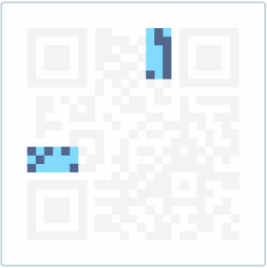
\includegraphics[width=.24\textwidth]{images/img04}}
		\caption{Información sobre la versión \cite{CitaA01}.}
		\label{fig:version}
	\end{center}
\end{figure}

Estos marcadores indican cuál de las 40 versiones del código QR está siendo usada. Normalmente las versiones utilizadas son de 1 a 7. \cite{CitaA01}\\

\title{Información del formato}

\begin{figure}[htbp]
	\begin{center}
		\fbox{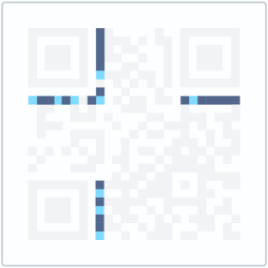
\includegraphics[width=.24\textwidth]{images/img05}}
		\caption{Información del formato \cite{CitaA01}.}
		\label{fig:formato2}
	\end{center}
\end{figure}

Contiene información sobre la tolerancia a los errores y el patrón del enmascaramiento de datos. La información sobre el formato facilita el escaneo del código. \cite{CitaA01}\\

\newpage
\title{Código de corrección de datos y errores}

\begin{figure}[htbp]
	\begin{center}
		\fbox{
\includegraphics[width=.24\textwidth]{images/img06}}
		\caption{Código de corrección de datos y errores \cite{CitaA01}.}
		\label{fig:erroresDatos}
	\end{center}
\end{figure}

El sistema de corrección de errores del código QR almacena toda la información y comparte el espacio con los módulos de corrección de errores, que permiten reconstruir los datos perdidos\cite{CitaA01} . \\

\title{Márgenes}

\begin{figure}[htbp]
	\begin{center}
		\fbox{
\includegraphics[width=.24\textwidth]{images/img07}}
		\caption{Márgenes \cite{CitaA01}}
		\label{fig:margenes}
	\end{center}
\end{figure}

Los márgenes, o también llamado zona quieta, alrededor del código QR son similares al espacio blanco en un diseño, proporcionan estructura y una mejor comprensión. Pero, ¿cómo? Para que el software de escaneo identifique bien el límite del código QR de sus alrededores, los márgenes son vitales.

\subsection{Fiabilidad de los códigos QR}
Los códigos QR están diseñados para mantener la información legible, aunque estén oscuros o dañados. Esto se logra mediante la compensación de errores, es decir, insertando la información varias veces. Con un alto nivel de seguridad, los códigos QR pueden leerse incluso si un tercio de su información es ilegible. Esto hace que los códigos QR sean muy fiables a la hora de guardar información. \\


%---------------------------------------------------------
% !TeX root = ../ejemplo.tex

\section{Desarrollo de la Aplicación Móvil}

Una aplicación móvil es un tipo de software diseñado para ejecutarse en dispositivos móviles, como teléfonos inteligentes o tabletas. A diferencia de las aplicaciones tradicionales para computadoras de escritorio, las aplicaciones móviles están optimizadas para operar con los recursos limitados de hardware de los dispositivos móviles, brindando funcionalidades específicas de manera eficiente. Aunque los dispositivos actuales son mucho más sofisticados que en sus primeras generaciones, las aplicaciones móviles siguen enfocándose en funciones concretas, permitiendo a los usuarios seleccionar solo las herramientas que necesitan en sus dispositivos \cite{IM1}.

Esta sección está enfocado en detallar el tipo de aplicación desarrollada para el proyecto, justificando las decisiones tecnológicas tomadas en cuanto a lenguajes, sistemas operativos y herramientas de desarrollo. Se explican los distintos tipos de aplicaciones móviles existentes, las razones detrás del uso de Kotlin y Android, así como las herramientas empleadas para su implementación.

\subsection{Tipos de aplicaciones móviles}
Existen diferentes tipos de aplicaciones móviles que responden a las necesidades y preferencias de los usuarios, así como a las capacidades técnicas de los dispositivos. A continuación, se detallan cada uno:

\begin{figure}[htbp]
	\begin{center}
		\fbox{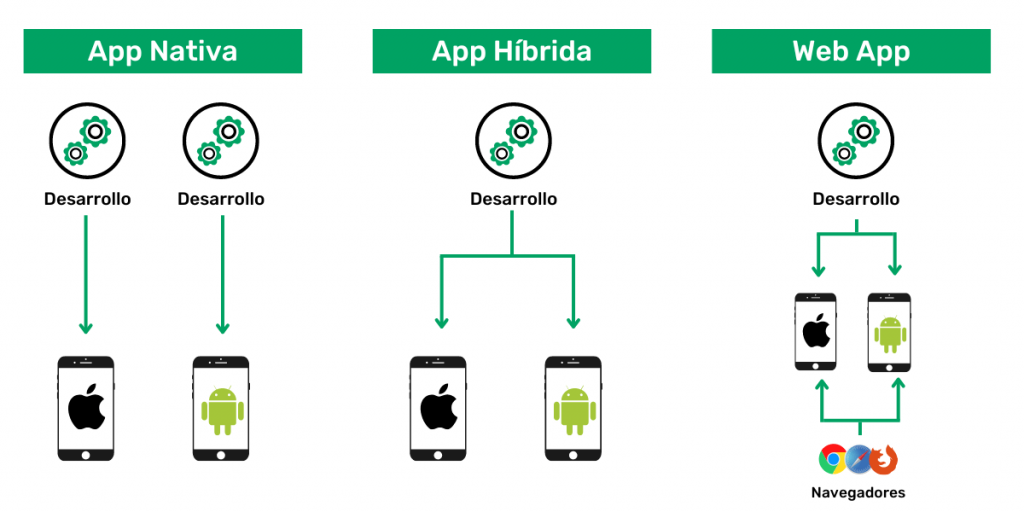
\includegraphics[width=.68\textwidth]{images/img08}}
		\caption{Tipo de aplicaciones moviles \cite{IM1}.}
		\label{fig:casosDeUso}
	\end{center}
\end{figure}

\subsection{Aplicaciones nativas}
Las aplicaciones nativas son apps desarrolladas para un sistema operativo móvil concreto (iOS o Android normalmente), en el lenguaje de programación específico de cada plataforma. Esto quiere decir que una app nativa creada para Android no puede ser utilizada en un dispositivo iOS y viceversa. \\

Es el tipo de aplicación móvil más conocida. Para que funcione, debemos descargarla desde los markets de apps, como App Store o Google Play e instalarla en nuestro teléfono \cite{CitaA02}.

\subsection*{Ventajas}
\begin{itemize}
	\item \textbf{Tienen el mejor rendimiento.} Las aplicaciones nativas son las más rápidas y tienen un rendimiento superior a otros tipos de apps, ya que han sido optimizadas específicamente para el hardware y el sistema operativo del dispositivo.
	\item \textbf{Acceso completo e integración con las funciones hardware del dispositivo.} Las apps nativas permiten aprovechar al máximo las funcionalidades móviles: cámara, micrófono, lector biométrico de huella, sensores y redes inalámbricas.
	\item \textbf{Pueden funcionar sin acceso a internet (funcionamiento offline)} si han sido diseñadas para ello.
\end{itemize}

\subsection*{Desventajas}
\begin{itemize}
	\item \textbf{Costes de desarrollo altos.} Si queremos tener nuestra app disponible para los dos sistemas, necesitaremos dos líneas de desarrollo diferentes, ya que el código utilizado para un sistema no es reutilizable para otro.
	\item \textbf{Complejidad de desarrollo.} Necesitamos equipos expertos en el lenguaje específico de cada sistema. Por ejemplo, en Kotlin para Android y en Swift para iOS.
	\item \textbf{Tiempo de desarrollo superior.} El desarrollo puede tomar entre 4 a 6 meses.
\end{itemize}

\subsection{Aplicaciones Web}

Las aplicaciones web realmente son webs especiales diseñadas para navegadores móviles. A diferencia de las apps nativas o híbridas, no necesitan ser descargadas, ya que se accede a ellas desde un navegador web.

Emplean las mismas tecnologías de desarrollo que una web, como HTML, CSS o JavaScript. Así, estaríamos hablando de una web con apariencia de app, por lo que presentaría sus mismas limitaciones. Sin embargo, con la llegada del HTML5, se han conseguido salvar algunas limitaciones, como el acceso a algunas funciones del móvil (geolocalización, cámaras) \cite{IM1}.

\subsection*{Ventajas}
\begin{itemize}
	\item \textbf{Carácter multiplataforma.} Con una sola línea de desarrollo.
	\item \textbf{Fácil desarrollo.} Se emplean tecnologías ampliamente conocidas.
	\item \textbf{Tiempo y coste de desarrollo bajo.}
\end{itemize}

\subsection*{Desventajas}
\begin{itemize}
	\item \textbf{Acceso limitado a las funciones del dispositivo.}
	\item \textbf{No se pueden subir a las tiendas de aplicaciones.}
	\item \textbf{Diferentes experiencias de usuario.} Estas dependen del navegador utilizado.
	\item \textbf{Necesidad de conexión a Internet.} Incluso si se cuenta con un modo pensado para ello, es necesario para acceder a las posibles actualizaciones o para entrar por primera vez.
\end{itemize}

\subsection{Aplicaciones Híbridas}

Las aplicaciones híbridas o multiplataforma combinan elementos de las aplicaciones nativas y las aplicaciones web. Estas aplicaciones se desarrollan utilizando tecnologías web como HTML, CSS y JavaScript, pero se empaquetan en un formato que puede ser instalado en un dispositivo móvil como cualquier otra aplicación nativa. Por tanto, podemos obtener una aplicación para varias plataformas con un único desarrollo \cite{IM1}.

\subsection*{Ventajas}
\begin{itemize}
	\item \textbf{Menor coste.} Gracias al uso de lenguajes de programación más conocidos, con una mayor disponibilidad de profesionales en el mercado.
	\item \textbf{Carácter multiplataforma.} Con una sola línea de desarrollo.
	\item \textbf{Acceso a algunas funcionalidades del móvil.}
	\item \textbf{Reducción de los tiempos de desarrollo.} Generalmente, el tiempo de desarrollo se reduce a 3 meses.
	\item \textbf{Disponibilidad en markets.} Se pueden subir a los markets de aplicaciones, como App Store y Google Play.
\end{itemize}

\subsection*{Desventajas}
\begin{itemize}
	\item \textbf{Rendimiento inferior.} Su rendimiento es inferior al de una app nativa, suelen tener un tamaño considerable y, además, ser más lentas.
	\item \textbf{Acceso limitado a las funciones del dispositivo.}
\end{itemize}

\subsection{Aplicaciones Progresivas Web Apps (PWA)}

Las aplicaciones progresivas son un reciente avance de las Web Apps. Al igual que las Web Apps, son webs diseñadas para móviles, pero esta vez, sí pueden ser descargadas en el móvil como una aplicación más, aunque no es necesario para que ofrezcan un comportamiento similar al de una app nativa a través del navegador. \\

Las PWA adoptan un comportamiento más propio de aplicaciones nativas que de web, como el funcionamiento sin Internet, un mayor rendimiento o su funcionamiento en segundo plano. Sin embargo, como desventaja, seguimos contando con la imposibilidad de subirlas a los markets de aplicaciones \cite{IM1}. \\

Para comprender mejor las diferencias entre los tipos de aplicaciones móviles, a continuación se presenta una tabla comparativa que destaca sus características clave:
\newpage

\begin{table}[h!]
	\centering
	\begin{tabular}{|p{4cm}|p{2cm}|p{2cm}|p{2cm}|}
		\hline
		\textbf{Tipos de app} & \textbf{Nativa} & \textbf{Híbrida} & \textbf{Web} \\ \hline
		\textbf{Interfaz} & Basada en web & Específica de la plataforma (iOS, Android) & Basada en web \\ \hline
		\textbf{Tiempo de desarrollo} & Alto & Medio & Bajo \\ \hline
		\textbf{Coste de desarrollo} & Alto & Medio & Bajo \\ \hline
		\textbf{Multiplataforma} & No & Sí & Sí \\ \hline
		\textbf{Rendimiento} & Alto & Medio & Bajo \\ \hline
		\textbf{Acceso a los sensores del dispositivo} & Completo & Alto o Completo & Limitado \\ \hline
		\textbf{Tiendas de aplicaciones} & Sí & Sí & No \\ \hline
	\end{tabular}
	\caption{Comparación tipos de aplicaciones móviles. Elaboración propia}
	\label{tab:tipos_apps}
\end{table}

Para el desarrollo de nuestro trabajo terminal, hemos decidido optar por una aplicación híbrida con el uso de Kotlin. Esta decisión se basa en varios factores relacionados con los recursos disponibles, las características de nuestro público objetivo y los plazos establecidos. \\

La aplicación móvil está dirigida para estudiantes, alumnos y personal de seguridad de la Escuela Superior de Cómputo, donde la mayoría utiliza dispositivos con sistema operativo Android. La elección de una aplicación híbrida nos permite optimizar  la experiencia en Android, que es la plataforma que predomina entre nuestros usuarios. \\

Aunque las aplicaciones híbridas suelen desarrollarse con tecnologías web (como React Native o Flutter), para nuestro proyecto hemos decidido incorporar Kotlin para desarrollar modelos donde se requiera un rendimiento nativo o un acceso más profundo a las funciones del sistema operativo Android.Además, las aplicaciones híbridas permiten un desarrollo más rápido en comparación con las aplicaciones completamente nativas, ya que gran parte del código puede compartirse entre plataformas, así mismo, es una buena opción económica que se adapta a nuestro presupuesto \cite{IM1}. 
%---------------------------------------------------------
% !TeX root = ../ejemplo.tex

\section{Elección de tecnología}
La elección de Kotlin como lenguaje principal y Android como plataforma se basa en criterios técnicos, prácticos y económicos que se alinean directamente con los requisitos del proyecto.

\subsection{Kotlin}
Kotlin es un lenguaje de alto nivel debido a su abstracción respecto al hardware y la plataforma subyacente. Esto significa que permite a los desarrolladores escribir código sin preocuparse por la gestión de memoria o las interacciones directas con el sistema operativo o el hardware, lo que mejora la productividad y la legibilidad del código, además, este es estáticamente tipado, lo que implica que los tipos de las variables se definen en tiempo de compilación, lo que permite detectar errores antes de ejecutar el programa. Este se usa principalmente en el desarrollo de aplicaciones Android, donde es el lenguaje recomendado por Google \cite{CitaD14}.

Además, Kotlin permite el uso de Jetpack Compose, un framework declarativo que moderniza la creación de interfaces de usuario en Android. También es compatible con bibliotecas clave para este proyecto como OpenCV, empleada en el módulo de reconocimiento facial.

\subsection{Android}
La decisión de desarrollar exclusivamente para Android se basa en:

\begin{itemize}
	\item La mayoría de los usuarios objetivo (alumnos, docentes y personal de seguridad) utilizan dispositivos Android.
	
	\item Android permite mayor flexibilidad y personalización, crucial para funciones como escaneo de códigos QR, acceso a la cámara, integración con Python y OpenCV.
	
	\item El entorno Android es ideal para pruebas, ya que se puede emular fácilmente en computadoras con Windows.
\end{itemize}

La compatibilidad de Android con Python facilita la integración del frontend (Android) con el backend, donde Python se encarga del procesamiento de imágenes y entrenamiento de modelos de reconocimiento facial, mientras que Spring Boot gestiona la lógica del sistema. Esta arquitectura garantiza un funcionamiento sincronizado, eficiente y seguro.


\section{Herramientas de Desarrollo}
El desarrollo de la aplicación se realizó con herramientas modernas que forman parte del ecosistema oficial de Android, permitiendo una implementación robusta y escalable.

\subsection{Android Studio}
Android Studio es el entorno de desarrollo integrado (IDE) oficial para el desarrollo de aplicaciones del mismo OS. Se basa en IntelliJ IDEA, un entorno de desarrollo integrado de Java para software, e incorpora sus herramientas de desarrollo y edición de código \cite{CitaD19}.

Para respaldar el desarrollo de aplicaciones dentro del sistema operativo, Android Studio utiliza un sistema de compilación basado en Gradle, un emulador de Android, plantillas de código e integración de GitHub. Cada proyecto en Android Studio tiene una o más modalidades con código fuente y archivos de recursos \cite{CitaD19}.

\subsection{Jetpack Compose}
Para la implementación de la aplicación móvil que forma parte de nuestro sistema de identificación y control de acceso, hemos decidido utilizar Jetpack Compose. La elección de la tecnología adecuada es importante para ofrecer una mejor experiencia de usuario y cumplir nuestros objetivos de diseño y funcional. 

\subsection*{¿Por que Jetpack compose?}
Jetpack compose es un framework (estructura o marco de trabajo que, bajo parámetros estandarizados, ejecutan tareas específicas en el desarrollo de un software) con la particularidad de ejecutar prácticas modernas en los desarrolladores de software a partir de la reutilización de componentes, así como también contando con la oportunidad de crear animaciones y temas oscuros. En este sentido, Jetpack Compose es el conjunto de herramientas ofrecidas por Android para el desarrollo de aplicaciones con un objetivo específico: simplificar y optimizar los códigos en la IU nativas \cite{CitaA01}. 


\subsection*{Ventajas}

\begin{itemize}
	\item \textbf{Menos código:} Simplifica el proceso de desarrollo haciendo menos código, todo se basa en funciones de modo que el código será simple y fácil de mantener.
	\item \textbf{Intuitiva:} Tan solo describe tu IU con un enfoque declarativo haciendo “qué hay que hacer” en vez de “cómo se debe hacer”.
	\item \textbf{Potente:} Tiene integrado Material Design con el cual puede crear apps atractivas al usuario con animaciones y mucho más.
	\item \textbf{Acelera el desarrollo:} Es compatible con proyectos existentes, puedes empezar a integrarlo por partes cuando quieras y donde quieras.
	\item \textbf{Kotlin:} Está escrito 100\% en Kotlin, lo cual nos permitirá usar sus herramientas potentes y API’s intuitivas.
\end{itemize}

\subsection*{Arquitectura Jetpack}
La arquitectura o estructura sobre la que se basa Jetpack Compose es una estructura Jetpack que se encarga principalmente de seguir ejecutando y beneficiándose de aquellos componentes de Android según la funcionalidad disponible. Por lo tanto, Jetpack Compose desarrolla herramientas denominadas «composables» a partir de elementos como botones o listados de objetos. A partir de fuentes de datos, pueden ser reutilizadas y ejecutadas en distintas fuentes sin la necesidad de programar varios códigos repetitivos.

Desde un aspecto comparativo, la creación de UI con Compose se realiza de forma similar a los de React Native. Es decir, mediante componentes reutilizables evitan maximizar la cantidad de códigos necesarios y repetitivos, tal como ocurre con HTML en la forma en la que se conjugan uno con otro. Sin embargo, es importante destacar que dicha compilación de componentes que logran la disminución en cantidad de códigos se realiza gracias a los plugins de compiladores de Kotlin, ejecutando así los componentes mediante la estructura de archivos de Kotlin \cite{CitaA19}. 

\subsection*{Estructura de Jetpack Compose}
Para entender de forma más sencilla la estructura de esta herramienta, conviene tener en cuenta componentes como:
\begin{itemize}
	\item \textbf{Compiler:} Se encarga mediante una estructura de plugins en Gradle, donde logra la interpretación y simplificación de códigos.
	\item \textbf{El entorno de ejecución:} Es el ámbito “depurador”, si se puede establecer de este modo, en el que se establecen y diferencian los componentes que necesitan actualización y cuáles no, así como también se crean listados de mantenimiento y composición.
	\item \textbf{UI:} Es el componente que interpreta el lenguaje establecido en el entorno de ejecución y lo refleja en pantalla.
\end{itemize}

\subsection{Gradle}

\begin{list}{}%
	{\setlength{\leftmargin}{1cm}\setlength{\rightmargin}{1cm}}
	\item\relax
	\small
	
	Gradle es el sistema de automatización de compilación utilizado por Android Studio, y fue esencial para el desarrollo del presente proyecto, permitiendo una integración fluida entre los módulos móviles y el backend. Esta herramienta de código abierto destaca por su rendimiento y flexibilidad, utilizando Kotlin DSL (Domain Specific Language) para definir scripts de compilación \cite{CitaD20}. 
	
	Gradle facilita la gestión eficiente de dependencias externas como Jetpack Compose, Retrofit y OpenCV, utilizadas en el desarrollo de la aplicación. Además, su capacidad para realizar compilaciones optimizadas en paralelo y reutilizar salidas anteriores permite reducir considerablemente los tiempos de construcción. También permite configurar distintos entornos de ejecución (debug y release), lo que fue útil para probar características específicas antes de su despliegue oficial. 
	
	En este proyecto, Gradle también permitió la integración con servicios backend mediante llamadas a APIs REST, conectando la aplicación con el servidor desarrollado en Spring Boot, fortaleciendo así la arquitectura cliente-servidor de la solución.
	
\end{list}

\subsection{Git y GitHub}

\begin{list}{}%
	{\setlength{\leftmargin}{1cm}\setlength{\rightmargin}{1cm}}
	\item\relax
	\small
	
	Durante el desarrollo del proyecto, se utilizó Git como sistema de control de versiones y GitHub como plataforma de colaboración y almacenamiento en la nube. Git, diseñado por Linus Torvalds, permite llevar un control detallado del historial de cambios en el código, lo cual es esencial en proyectos donde trabajan varios desarrolladores de forma simultánea \cite{CitaD20}.
	
	Cada miembro del equipo pudo trabajar en ramas independientes, realizar modificaciones, proponer mejoras y fusionar los cambios mediante revisiones de código, garantizando la integridad del repositorio principal. Esta metodología permitió detectar errores, revertir versiones cuando fue necesario, y mantener una trazabilidad clara del desarrollo de cada módulo.
	
	GitHub, además de servir como repositorio central, funcionó como herramienta de comunicación y documentación del avance del proyecto. Las funcionalidades de issues, pull requests y proyectos ayudaron a distribuir tareas, dar seguimiento a problemas y mantener una organización clara durante todo el ciclo de desarrollo \cite{CitaD21}.
	
\end{list}



%---------------------------------------------------------
% !TeX root = ../ejemplo.tex

\section{Lenguaje de programación}

Una vez establecido el sistema operativo que vamos a usar, nos interesa establecer que es un lenguaje de programación.
\begin{list}{}%
    {\setlength{\leftmargin}{1cm}\setlength{\rightmargin}{1cm}}
    \item\relax
    \small
En términos generales, un lenguaje de programación es una herramienta que permite desarrollar software o programas para computadora. Los lenguajes de programación son empleados para diseñar e implementar programas encargados de definir y administrar el comportamiento de los dispositivos físicos y lógicos de una computadora. Lo anterior se logra mediante la creación e implementación de algoritmos de precisión que se utilizan como una forma de comunicación humana con la computadora \cite{CitaD10}.

A grandes rasgos, un lenguaje de programación se conforma de una serie de símbolos y reglas de sintaxis y semántica que definen la estructura principal del lenguaje y le dan un significado a sus elementos y expresiones \cite{CitaD10}.
\end{list}
Estos se dividen en 3 tipos: lenguajes máquina, lenguajes de bajo nivel y lenguajes de alto nivel.


\subsection{Lenguajes máquina}

\begin{list}{}%
    {\setlength{\leftmargin}{1cm}\setlength{\rightmargin}{1cm}}
    \item\relax
    \small

Es el sistema de códigos interpretable directamente por un circuito microprogramable, como el microprocesador de una computadora. Este lenguaje se compone de un conjunto de instrucciones que determinan acciones que serán realizadas por la máquina. Y un programa de computadora consiste en una cadena de estas instrucciones de lenguaje de máquina (más los datos). Normalmente estas instrucciones son ejecutadas en secuencia, con eventuales cambios de flujo causados por el propio programa o eventos externos. El lenguaje máquina es específico de cada máquina o arquitectura de la máquina, aunque el conjunto de instrucciones disponibles pueda ser similar entre ellas \cite{CitaD10}.

\end{list}

\subsection{Lenguajes de alto nivel}

\begin{list}{}%
    {\setlength{\leftmargin}{1cm}\setlength{\rightmargin}{1cm}}
    \item\relax
    \small

Un lenguaje de programación de bajo nivel es el que proporciona poca o ninguna abstracción del microprocesador de una computadora. Consecuentemente, su trasladado al lenguaje máquina es fácil. El término ensamblador (del inglés assembler) se refiere a un tipo de programa informático encargado de traducir un archivo fuente, escrito en un lenguaje ensamblador, a un archivo objeto que contiene código máquina ejecutable directamente por la máquina para la que se ha generado \cite{CitaD10}. 

\end{list}

\subsection{Lenguajes de bajo nivel}

\begin{list}{}%
    {\setlength{\leftmargin}{1cm}\setlength{\rightmargin}{1cm}}
    \item\relax
    \small

Los lenguajes de programación de alto nivel se caracterizan porque su estructura semántica es muy similar a la forma como escriben los humanos, lo que permite codificar los algoritmos de manera más natural, en lugar de codificarlos en el lenguaje binario de las máquinas, o a nivel de lenguaje ensamblador \cite{CitaD10}. 

\end{list}

Entre estos tipos de lenguajes nos interesa los lenguajes de alto nivel ya que para el proyecto estamos considerando el uso de Python, Java y Kotlin, que son considerados lenguajes de alto nivel. Concretamente Python es un lenguaje multiparadigma que puede ser estructurado como si se usara la programación orientada a objetos, Java usa la programación orientada a objetos y Kotlin puede trabajar con esta orientación por lo que antes de definir qué son estos dos lenguajes es de vital importancia definir qué es la “programación orientada a objetos”.


\subsection{Programación orientada a objetos}

\begin{list}{}%
    {\setlength{\leftmargin}{1cm}\setlength{\rightmargin}{1cm}}
    \item\relax
    \small

La programación orientada a objetos (POO) es un modelo de programación informática que organiza el diseño del software en torno a datos u objetos, en lugar de funciones y lógica. Un objeto puede definirse como un campo de datos que tiene unos atributos y comportamientos únicos\cite{CitaD11}.
Los ejemplos de un objeto pueden ir desde entidades físicas, como un ser humano que se describe por propiedades como el nombre y la dirección, hasta pequeños programas informáticos, como los widgets\cite{CitaD11}.
La POO se centra en los objetos que los desarrolladores quieren manejar, en lugar de la lógica necesaria para hacerlo. Este enfoque de la programación es muy adecuado para programas grandes, complejos y que se actualizan o mantienen activamente\cite{CitaD11}.
Esto incluye programas para la producción y el diseño web, así como aplicaciones móviles\cite{CitaD11}.

\end{list}

\subsection{Python}

\begin{list}{}%
    {\setlength{\leftmargin}{1cm}\setlength{\rightmargin}{1cm}}
    \item\relax
    \small

En términos técnicos, Python es un lenguaje de programación de alto nivel, orientado a objetos, con una semántica dinámica integrada, principalmente para el desarrollo web y de aplicaciones informáticas, o a nivel de lenguaje ensamblador\cite{CitaD12}.
Python es relativamente simple, por lo que es fácil de aprender, ya que requiere una sintaxis única que se centra en la legibilidad. Los desarrolladores pueden leer y traducir el código Python mucho más fácilmente que otros lenguajes\cite{CitaD12}.
Por tanto, esto reduce el costo de mantenimiento y de desarrollo del programa porque permite que los equipos trabajen en colaboración sin barreras significativas de lenguaje y experimentación\cite{CitaD12}.
Además, soporta el uso de módulos y paquetes, lo que significa que los programas pueden ser diseñados en un estilo modular y el código puede ser reutilizado en varios proyectos. Una vez se ha desarrollado un módulo o paquete, se puede escalar para su uso en otros proyectos, y es fácil de importar o exportar\cite{CitaD12}.
Por otro lado, uno de los beneficios más importantes de Python es que tanto la librería estándar como el intérprete están disponibles gratuitamente, tanto en forma binaria como en forma de fuente\cite{CitaD12}.
Tampoco hay exclusividad, ya que Python y todas las herramientas necesarias están disponibles en todas las plataformas principales \cite{CitaD12}.

\end{list}


\subsection{Java}

\begin{list}{}%
    {\setlength{\leftmargin}{1cm}\setlength{\rightmargin}{1cm}}
    \item\relax
    \small

Java es un lenguaje orientado a objetos; es decir que organiza el trabajo en torno a objetos en lugar de funciones y lógica. Las aplicaciones móviles y herramientas de software, incluidos los mundialmente famosos Amazon, Spotify y Minecraft, se basan en Java.
Java tiene dos propiedades que determinan qué tareas se pueden resolver con él.
Java es un lenguaje de programación orientado a objetos (POO). Toda interacción en él se produce a través de objetos. Estas entidades se describen en código y se les enseña a interactuar entre sí. Como resultado, un programa de estilo orientado a objetos consta de bloques separados que son fácilmente extensibles y escalables. \cite{CitaD13}

\end{list}

Y java tiene la capacidad de interpretar y compilar, es decir tiene un intérprete que se dedica a leer cada línea de código una por una y ejecutarla sin traducirla a lenguaje máquina y además puede transformar su código  a lenguaje máquina y hacer que el procesador lo compile traducido \cite{CitaD13}. 


\subsection{Kotlin}

Kotlin es un lenguaje de alto nivel debido a su abstracción respecto al hardware y la plataforma subyacente. Esto significa que permite a los desarrolladores escribir código sin preocuparse por la gestión de memoria o las interacciones directas con el sistema operativo o el hardware, lo que mejora la productividad y la legibilidad del código, además, este es estáticamente tipado, lo que implica que los tipos de las variables se definen en tiempo de compilación, lo que permite detectar errores antes de ejecutar el programa. Este se usa principalmente en el desarrollo de aplicaciones Android, donde es el lenguaje recomendado por Google \cite{CitaD14}.

Con la información anterior se puede explicar porque consideramos estos tres lenguajes de programación; Primero estos tres lenguajes poseen una misma orientación lo cual nos ayuda a que el desarrollo del proyecto sea más conciso y fácil, después estos son lenguajes de alto nivel que tienen una buena legibilidad lo que le permite al equipo entender de manera más sencilla el trabajo de los demás integrantes, también pueden ser conectados entre ellos de manera relativamente fácil y sobretodo su alta cantidad de bibliotecas de apoyo y su características de ser  estándares de desarrollo; en android (Kotlin), de desarrollo para servidores (Python) y Java para desarrollo web.
Otra razón por la que decidimos usar estos tres lenguajes de programación es por su compatibilidad con la API OpenCV la cual será una herramienta clave para el desarrollo de nuestro proyecto, por lo que es necesario explicar que es una API y qué es OpenCV.

%---------------------------------------------------------
% !TeX root = ../ejemplo.tex

\section{API}

\begin{list}{}%
    {\setlength{\leftmargin}{1cm}\setlength{\rightmargin}{1cm}}
    \item\relax
    \small

Una API, o interfaz de programación de aplicaciones, es un conjunto de reglas o protocolos que permiten que las aplicaciones de software se comuniquen entre sí para intercambiar datos, características y funcionalidades \cite{CitaD15}.
Las API simplifican y aceleran el desarrollo de software y aplicaciones permitiendo a los desarrolladores integrar datos, servicios y capacidades de otras aplicaciones, en lugar de desarrollarlas desde cero. Las API también ofrecen a los propietarios de aplicaciones una forma sencilla y segura de poner los datos y las funciones de sus aplicaciones a disposición de los departamentos de su organización. Los propietarios de aplicaciones también pueden compartir o comercializar datos y funciones con asociados de negocios o terceros [24].

\end{list}

\subsection{OpenCV}

\begin{list}{}%
    {\setlength{\leftmargin}{1cm}\setlength{\rightmargin}{1cm}}
    \item\relax
    \small

OpenCV, o Open Source Computer Vision Library, es una colección de más de 2500 algoritmos optimizados que facilitan el procesamiento de imágenes y la realización de diversas operaciones de vision computacional. Fundada por Intel en 2000 y con colaboración de múltiples empresas y desarrolladores, esta biblioteca es de fácil acceso y cuenta con una licencia BSD [25].
Siendo compatible con varios lenguajes de programación, incluido Python, Java y C++, OpenCV permite trabajar en múltiples plataformas y sistemas operativos. Esta biblioteca también destaca por su papel en el impulso de tecnologías emergentes como el deep learning \cite{CitaD16}.

\end{list}

Por último esta cuenta con muchos procesos y funciones que apoyan al reconocimiento facial, además de ser compatible con Python, Kotlin y Java y poseer una alta cantidad de tutoriales que rondan desde las integraciones básicas hasta procesos avanzados.

\subsection{Licencia BSD}

\begin{list}{}%
    {\setlength{\leftmargin}{1cm}\setlength{\rightmargin}{1cm}}
    \item\relax
    \small

"La licencia BSD, también conocida como licencia de distribución de software de Berkeley, es una popular licencia de código abierto que permite el libre uso, modificación y distribución de software \cite{CitaD17}."

\end{list}

Esta licencia nos permite hacer uso de la biblioteca OpenCV de manera libre, lo cual implica que se puede implementar la biblioteca y darle uso al software de manera comercial, nos permite modificar y distribuir el software sin restricciones significativas y nos permite no publicar el código fuente si así lo deseamos.

Ya con el sistema operativo y los lenguajes de programación establecidos, tenemos que especificar las herramientas que nos permitirán escribir, depurar y gestionar el código de manera eficiente. Estas herramientas son los entornos de desarrollo Integrados (IDE, por sus siglas en inglés), que proporcionan un conjunto de funciones como editores de código, depuradores, y compiladores.


%---------------------------------------------------------
% !TeX root = ../ejemplo.tex

\section{IDE}

Un entorno de desarrollo integrado (IDE) es un sistema de software para el diseño de aplicaciones que combina herramientas del desarrollador comunes en una sola interfaz gráfica de usuario (GUI). Generalmente, un IDE cuenta con las siguientes características \cite{CitaD18}:

\begin{list}{}%
    {\setlength{\leftmargin}{1cm}%
     \setlength{\rightmargin}{1cm}%
     \setlength{\itemsep}{0.5\baselineskip}%
     \setlength{\parsep}{0pt}}
     
    \item\relax
    \small
    \textbf{Editor de código fuente:} editor de texto que ayuda a escribir el código de software con funciones como el resaltado de la sintaxis con indicaciones visuales, el relleno automático específico para el lenguaje y la comprobación de errores a medida que se escribe el código \cite{CitaD18}.
    \textbf{Automatización de las compilaciones locales:} herramientas que automatizan las tareas sencillas y repetitivas como parte de la creación de una compilación local del software para que use el desarrollador, como la compilación del código fuente de la computadora en código binario, el empaquetado de ese código y la ejecución de pruebas automatizadas \cite{CitaD18}.
    \textbf{Depurador:} programa que sirve para probar otros programas y mostrar la ubicación de un error en el código original de forma gráfica \cite{CitaD18}.

\end{list}

Para nuestro proyecto ocuparemos el IDE llamado android studio.

\subsection{Android Studio}

\begin{list}{}%
    {\setlength{\leftmargin}{1cm}\setlength{\rightmargin}{1cm}}
    \item\relax
    \small

Android Studio es el entorno de desarrollo integrado (IDE) oficial para el desarrollo de aplicaciones del mismo OS. Se basa en IntelliJ IDEA, un entorno de desarrollo integrado de Java para software, e incorpora sus herramientas de desarrollo y edición de código \cite{CitaD19}.

Para respaldar el desarrollo de aplicaciones dentro del sistema operativo, Android Studio utiliza un sistema de compilación basado en Gradle, un emulador de Android, plantillas de código e integración de GitHub. Cada proyecto en Android Studio tiene una o más modalidades con código fuente y archivos de recursos \cite{CitaD19}.

\end{list}


\subsection{Gradle}

\begin{list}{}%
    {\setlength{\leftmargin}{1cm}\setlength{\rightmargin}{1cm}}
    \item\relax
    \small

Gradle, es una herramienta que permite la automatización de compilación de código abierto, la cual se encuentra centrada en la flexibilidad y el rendimiento. Los scripts de compilación de Gradle se escriben utilizando Kotlin DSL (Domain Specific Language) \cite{CitaD20}.
Gradle tiene una gran flexibilidad y nos deja hacer usos de otros lenguajes y no solo de Java, también cuenta con un sistema de gestión de dependencias muy estable. Gradle es altamente personalizable y rápido ya que completa las tareas de forma rápida y precisa reutilizando las salidas de las ejecuciones anteriores, sólo procesar las entradas que presentan cambios en paralelo \cite{CitaD20}.
Además es el sistema de compilación oficial para Android y cuenta con soporte para diversas tecnologías y lenguajes \cite{CitaD20}.

\end{list}


\subsection{GitHub}

\begin{list}{}%
    {\setlength{\leftmargin}{1cm}\setlength{\rightmargin}{1cm}}
    \item\relax
    \small

GitHub es una plataforma de desarrollo colaborativo que aloja proyectos en la nube utilizando el sistema de control de versiones llamado Git. Ayuda a los desarrolladores a almacenar y administrar el código llevando un registro de cambios. Generalmente el código es abierto, lo que permite realizar proyectos compartidos y mantener el seguimiento detallado de su progreso. La plataforma GitHub también funciona como red social conectando a los desarrolladores con los usuarios. Como usuario puedes descargar programas o aplicaciones, y de la misma manera puedes aportar a su desarrollo ofreciendo mejoras y discutir las cuestiones que te interesan en foros temáticos \cite{CitaD21}.
\end{list}

\subsection{Git}

\begin{list}{}%
    {\setlength{\leftmargin}{1cm}\setlength{\rightmargin}{1cm}}
    \item\relax
    \small

Git es un software de control de versiones diseñado por Linus Torvalds, el creador de Linux. El propósito de Git es llevar un registro de cambios y coordinar el trabajo de varias personas en un repositorio compartido. Desde su creación en 2005, este software llegó a convertirse en uno de los VCS más populares: según la encuesta de Stack Overflow (en inglés), más del noventa porciento de los desarrolladores usan Git en sus proyectos \cite{CitaD20}.
Git proporciona herramientas para un trabajo rápido y eficiente dentro de un equipo. El control de versiones permite a los desarrolladores descargar una copia del código fuente a sus repositorios locales (PC), realizar cambios y subir una versión nueva al repositorio compartido. Todas las modificaciones se guardan en versiones independientes, sin afectar el archivo original. Se pueden comparar cambios realizados, ver quién modificó el código y determinar en qué momento se introdujo un error para poder revertirlo. De esta forma todos los desarrolladores interesados en el proyecto tienen acceso al historial de modificaciones realizadas y pueden contribuir mejorando el código del software \cite{CitaD21}.

\end{list}

Esta última es una herramienta que tenemos planeada usar para el control de versiones en nuestro proyecto. 

%---------------------------------------------------------
% !TeX root = ../ejemplo.tex

\section{Framework}
\subsection{Jetpack compose}
Para la implementación de la aplicación móvil que forma parte de nuestro sistema de identificación y control de acceso, hemos decidido utilizar Jetpack Compose. La elección de la tecnología adecuada es importante para ofrecer una mejor experiencia de usuario y cumplir nuestros objetivos de diseño y funcional. 

\subsection*{¿Por que Jetpack compose?}
Jetpack compose es un framework (estructura o marco de trabajo que, bajo parámetros estandarizados, ejecutan tareas específicas en el desarrollo de un software) con la particularidad de ejecutar prácticas modernas en los desarrolladores de software a partir de la reutilización de componentes, así como también contando con la oportunidad de crear animaciones y temas oscuros. En este sentido, Jetpack Compose es el conjunto de herramientas ofrecidas por Android para el desarrollo de aplicaciones con un objetivo específico: simplificar y optimizar los códigos en la IU nativas \cite{CitaA01}. 


\subsection*{Ventajas}

\begin{itemize}
	\item \textbf{Menos código:} Simplifica el proceso de desarrollo haciendo menos código, todo se basa en funciones de modo que el código será simple y fácil de mantener.
	\item \textbf{Intuitiva:} Tan solo describe tu IU con un enfoque declarativo haciendo “qué hay que hacer” en vez de “cómo se debe hacer”.
	\item \textbf{Potente:} Tiene integrado Material Design con el cual puede crear apps atractivas al usuario con animaciones y mucho más.
	\item \textbf{Acelera el desarrollo:} Es compatible con proyectos existentes, puedes empezar a integrarlo por partes cuando quieras y donde quieras.
	\item \textbf{Kotlin:} Está escrito 100\% en Kotlin, lo cual nos permitirá usar sus herramientas potentes y API’s intuitivas.
\end{itemize}
%---------------------------------------------------------
% !TeX root = ../ejemplo.tex
%---------------------------------------------------------
% !TeX root = ../ejemplo.tex

\section{Bases de datos (BD)}
Para que todo sistema pueda funcionar, debe de tener una forma de almacenar toda su información, ya sea información de los usuarios o para almacenar imágenes, cualquier tipo de información que se requiera almacenar, es necesario usar una base de datos. Pero en sí, ¿qué es una base de datos?.
Una base de datos, según Microsoft \cite{CitaAJ08} , es una herramienta para recopilar y organizar información. Estas pueden almacenar información sobre personas, productos, pedidos u otras cosas. Las bases de datos pueden empezar desde un simple documento de textos o archivos Excel, pero conforme más va creciendo esta base de datos empiezan a aparecer redundancias, por lo que es mejor optar por usar una base de datos creada por un sistema gestor de bases de datos. 
Un sistema gestor de bases de datos es un software constituido por una serie de programas dirigidos a crear, gestionar y administrar la información que se encuentra en una base de datos. El principal objetivo de estos sistemas es servir de interfaz entre los usuarios y las aplicaciones para facilitar la organización de los datos \cite{CitaAJ06}.
Por otro lado, dentro del mundo de las bases de datos, existen diferentes tipos de bases de datos, y cada tipo de base de datos tiene una organización diferente y propósito diferente. A continuación, les hablaremos de ciertos tipos de bases de datos:

\subsection{Bases de datos relacionales:}
Este tipo de bases de datos es el más usado en sistemas que necesitan almacenar una gran cantidad de información que está relacionada entre sí. Ahora bien, una base de datos relacional, según Google \cite{CitaAJ09}, es una forma de estructurar información en tablas, filas y columnas. La ventaja de este tipo de bases de datos es que tiene la capacidad de establecer relaciones entre la información mediante tablas, esto nos ayuda a visualizar mejor la información sobre la relación entre los datos.
Las bases de datos relacionales se componen de una serie de conceptos clave que necesitamos desarrollar para mejorar la comprensibilidad acerca de este tipo de bases de datos:

\begin{itemize}
    \item \textbf{Tablas:} Las tablas, en una base de datos relacional, son objetos que contienen todos los datos de dicho objeto. Como se mencionó anteriormente, estas tablas se organizan en filas y columnas. Aquí, cada fila representa un registro único y cada columna un campo dentro del registro. La manera en que este tipo de tablas guardan datos únicos es por medio de una clave principal, la cuál se va a explicar a continuación. \cite{CitaAJ10}
    \item \textbf{Clave principal:} Como ya se mencionó, las tablas tienen una clave principal, la cuál suele ser una columna o un conjunto de columnas cuyos valores identifican la forma única de cada fila de la tabla. Estas columnas se denominan claves principales de la tabla y aunque la clave principal sea una combinación de columnas, esta combinación es única dentro de la tabla. \cite{CitaAJ11}
    \item \textbf{Clave externa:} Esta es una columna o combinación de columnas que se usa para establecer un vínculo entre los datos de dos tablas. Cuando una tabla tiene dentro de sus columnas la clave principal de otra tabla, se dice que esa primera tabla está referenciando a la otra por medio de una clave externa. \cite{CitaAJ12}
    \item \textbf{Sistema de gestión de bases de datos (SGBD):} Son sistemas que ayudan a controlar las bases de datos. Estos sistemas actúan como interfaz entre los usuarios y las bases de datos, y se encargan justamente de gestionar los datos y las bases de datos como tal. En otras palabras, un sistema de gestión de bases de datos es un software utilizado para gestionar, almacenar y recuperar bases de datos, a su vez, proporciona una interfaz que permite a los usuarios leer, crear, borrar y actualizar datos. \cite{CitaAJ06}
\end{itemize}

\subsubsection{PostgreSQL:}
PostgreSQL es una SGBD relacional, el cual, a diferencia de otros este soporta tipos de datos relacionales y no relacionales. Este fue creado con el propósito de soportar cagras de trabajo desde pequeñas aplicaciones hasta sistemas complejos de procesamiento de datos a gran escala. 
Para este proyecto, se hará uso de este SGBD, ya que tiene compatibilidad con los diferentes lenguajes que vamos a usar, como lo es Java, y además, es libre de restricciones de licencia. \cite{CitaAJ05}

\subsection{Bases de datos no relacionales:}
Este tipo de bases de datos no siguen el esquema de filas y columnas como las bases de datos relacionales, en su lugar, este tipo de bases de datos usan un modelo de almacenamiento que está optimizado para los requisitos del tipo de dato que van a guardar. Dentro de este tipo de bases de datos existe una gran variedad, hay bases de datos que almacenan su información como pares clave/valor simple, como formatos JSON, o como un grafo que consta de bordes y vértices. Lo que caracteriza a este tipo de bases de datos es que no usan el modelo relacional. \cite{CitaAJ12}

%---------------------------------------------------------
% !TeX root = ../ejemplo.tex

\section{Spring Boot}
Spring Boot es una herramienta que sirve para desarrollar tanto aplicaciones web, como microservicios en Java. Este se basa en Spring Framework, el cual es un framework para el desarrollo de aplicaciones y contenedores de inversión de control de código abierto, igualmente para Java.
Spring Boot permite el desarrollo de aplicaciones web y microservicios de manera rápida y fácil gracias a 3 características que tiene, las cuales son:
\begin{itemize}
    \item \textbf{Configuración automática:} Con esto se refiere a que Spring Boot lo que hace es analizar las dependencias incluidas en un proyecto, como lo son bases de datos, servidores, entre otras cosas y decide qué configuraciones aplicar. Esto se basa en anotaciones que usualmente empiezan con un "@", gracias a esto, podemos desarrollar aplicaciones de manera más rápida y eficiente, pues nos ahorra todo el trabajo de realizar método por método. \cite{CitaAJ01}
    \item \textbf{Enfoque obstinado de la configuración:} Con base en las mejores prácticas de la programación, Spring Boot toma ciertas decisiones de configuración que funcionan bien para la mayoría de casos, esto se refiere a configuraciones de puertos, rutas, entre otras cosas. Además, en caso de que nosotros queramos agregar configuraciones adicionales, o bien, cambiar la configuración de algo de nuestro proyecto, nos va a crear un archivo de configuración en donde podremos especificarle de qué manera lo queremos. \cite{CitaAJ02}
    \item \textbf{Capacidad de crear aplicaciones independientes:} Nos permite crear aplicaciones que se ejecutan de forma independiente, es decir, sin necesidad de un servidor web externo. Esto lo logra gracias a que en el proceso de inicialización, se integra un servidor web en la aplicación, o que le permite funcionar de manera autónoma. \cite{CitaAJ01}
\end{itemize}

\section{Java Persistence API (JPA)}
Antes de irnos a la definición de JPA, hay que entender qué es la persistencia de los datos. La persistencia de los datos es un medio mediante el cual una aplicación puede recuperar información desde un sistema de almacenamiento y hacer que esta persista. Ahora bien, JPA lo que hace es proporcionarnos varias funciones para poder gestionar la persistencia y la correlación de objetos, es decir, lo que hace es proveernos con una serie de interfaces que podemos utilizar para implementar la capa de persistencia de nuestra aplicación. \cite{CitaAJ03}

Algunas de las ventajas que nos presenta JPA es que nos permite hacer el mapeo de entidades, es decir, el definir cómo se relacionan las clases de nuestra aplicación con los elementos de nuestra base de \cite{CitaAJ03}. Esto abarca temas como las relaciones entre clases y tablas en nuestra abse de datos, propiedades de las clases y los campos de las tablas e incluso la relación entre diferentes clases y las claves exrternas de nuestras tablas. 

Además, JPA ofrece la capacidad de interactuar con diferentes sistemas de gestión de bases de datos, ya que no usa sentencias SQL o de algún tipo de base de datos en específico, por lo que mejora la portabilidad y escalabilidad de las aplicaciones. \cite{CitaAJ04}
%---------------------------------------------------------
% !TeX root = ../ejemplo.tex

\section{Patrones de arquitectura de software}
Al momento de desarrollar software, es común toparnos con problemáticas que requieren de la toma de decisiones especialmente cuando hablamos sobre cuestiones relacionadas con el diseño de un sistema de software.
Un patrón de arquitectura de software es un conjunto de decisiones tomadas para atacar problemáticas relacionadas con el diseño de un software. Estos incluyen reglas y principios para organizar las interacciones entre subsistemas predefinidos y los roles que estos desempeñan \cite{L07}.

A menudo pueden ser descritos como los \textit{"Planos"} de un sistema, sin embargo, esto no quiere decir que sea la arquitectura final, sino que funcionan como una guía que describe los elementos necesarios para diseñar la arquitectura de la solución a desarrollar, la selección de una arquitectura sobre otra dependerá completamente de los objetivos a alcanzar, los recursos disponibles y la experiencia del equipo de desarrollo \cite{L08}.

Es necesario aclarar que, los patrones de arquitectura no deben confundirse con los patrones de diseño, ya que ambos responden a problemas diferentes durante el desarrollo de un sistema de software, de forma muy breve un patrón de arquitectura describe como crear la lógica de negocio, acceso a los datos, etc. Mientras que los patrones de diseño se usan al implementar estos elementos \cite{L07}.

A continuación, se describen algunos patrones de arquitectura que pueden ser de utilidad al implementar la propuesta de solución para este trabajo terminal.	

\subsection{Arquitectura de capas}

También conocida como \textit{arquitectura de N-capas}, estructura una aplicación en múltiples capas distintas, donde cada una esta encargada de ciertas tareas en especifico, lo que permite dividir un sistema en componentes aislados, lo que facilita el desarrollo rápido de aplicaciones ya que los cambios realizados en una capa no deberían afectar la lógica de las demás \cite{L09}.

Las arquitecturas basadas en este patrón suelen implementar cuatro capas distintas, la capa de presentación, la capa de negocio, de persistencia y de base de datos, sin embargo, y como es de esperarse, la arquitectura de un sistema basado en este patrón puede tener algunas diferencias en el número y tipo de capas que se implementan, por ejemplo, algunas pueden implementar capas de aplicación, servicio o acceso a datos \cite{L07}.

\subsection{Arquitectura orientada a servicios}

Las aplicaciones diseñadas siguiendo este patrón de arquitectura implementan una colección de servicios poco acoplados que se comunican entre sí a través de una red.
Cada uno de los servicios que conforman al sistema se encarga de llevar acabo una función del negocio en específico que después pueden ser requeridos por otro servicio o cliente \cite{L09}.


\subsection{Arquitectura de micro servicios}

Es una arquitectura que combina patrones de diseño para crear múltiples servicios que trabajan de forma independiente y que en conjunto forman la lógica de una aplicación. Es una alternativa a las aplicaciones monolíticas y de la arquitectura basada en servicios, en donde cada servicio esta orientado a implementar partes muy puntuales de la lógica de negocio \cite{L08}.

Su principal ventaja radica en que debido a que sus componentes se encuentran poco acoplados pueden ser desarrollados, desplegados y probados de forma independiente \cite{L09}.

La principal desventaja de este tipo de arquitectura es que puede llegar a ser compleja de implementar ya que requiere de definir la granularidad correcta de los servicios y establecer una comunicación efectiva entre estos \cite{L07}.

\subsection{El patrón modelo vista controlador}

Este patrón divide divide una aplicación en tres componentes interconectados. El modelo, la vista y el controlador. Esta separación permite organizar el código al desacoplar la lógica del negocio, interfaz de usuario y el manejo de las entradas de los usuarios, lo que a su vez promueve la modularidad, mantenibilidad y escalabilidad \cite{L09}. 

El modelo contiene los datos y lógica de negocio de la aplicación. Se encarga de regresar, almacenar y procesar la información.

La vista, también conocida como interfaz de usuario (UI) despliega la información al usuario y responde a las interacciones del usuario.

El controlador funciona como un intermediario entre el modelo y la vista. Se encarga de gestionar las entradas del usuario, actualizar el modelo y la vista para reflejar los cambios realizados en el modelo \cite{L08}.

%---------------------------------------------------------
% !TeX root = ../ejemplo.tex

\section{Redes neuronales artificiales}

Una red neuronal artificial es una técnica para la creación de programas de computación que son capaces de aprender de los datos. Se basa en el conocimiento actual sobre como funciona el cerebro humano. 
Consisten en un conjunto de nodos o neuronas interconectados entre sí que procesan y aprenden de los datos con los que cuentan, lo que permite llevar a cabo tareas como el reconocimiento de patrones y la toma de decisiones en el aprendizaje de máquina \cite{L10}.


\subsection{Estructura de una red neuronal artificial}
Toda red neuronal esta formada por capas de nodos, o neuronas artificiales, una capa de entrada, una o más capas ocultas y una capa de salida. Cada nodo se conecta a los demás y tiene un peso y un umbral determinado.
A continuación se describe el papel que cada una de estas capas en la arquitectura de una red neuronal común \cite{L11}.

\subsubsection{Capa de entrada}
La capa de entrada es responsable de recibir los datos iniciales en forma de vectores. Cada neurona en esta capa corresponde a una característica del conjunto de datos \cite{L12}.

\subsubsection{Capas ocultas}
Las capas ocultas son el núcleo de las RNA y donde ocurre el procesamiento de los datos. Estas capas aplican transformaciones no lineales mediante funciones de activación, como \textit{ReLU}, \textit{sigmoide}, o \textit{tangente hiperbólica}. El número y tamaño de las capas ocultas determinan la capacidad de la red para modelar patrones complejos \cite{L12}.

\subsubsection{Capa de salida}
La capa de salida genera los resultados finales del modelo. Para tareas de clasificación, por ejemplo, esta capa utiliza funciones como \textit{softmax} para proporcionar probabilidades asociadas a cada clase \cite{L12}.

\section{Proceso de aprendizaje}
Como ya se mencionó con anterioridad, una red neuronal es un sistema complejo que busca imitar la forma en la que el cerebro humano aprende \cite.
Este proceso de aprendizaje se realiza en dos fases conocidas como \textit{backpropagation} y \textit{forward propagation} \cite{L12}:


\subsection{Forward propagation}

\begin{itemize}
	\item \textbf{Capa de entrada:} La capa de entrada contiene nodos que representan cada característica del conjunto de datos inicial. Estos nodos reciben y procesan los datos de entrada.  
	\item \textbf{Pesos y conexiones:} Los pesos asignados a cada conexión entre neuronas determinan la influencia de una neurona sobre otra. Durante el entrenamiento, estos valores se actualizan constantemente para optimizar el rendimiento de la red.  
	\item \textbf{Capas ocultas:} Las neuronas en las capas ocultas combinan las entradas recibidas al multiplicarlas por sus respectivos pesos y sumarlas. Posteriormente, aplican una función de activación que introduce no linealidad, lo que permite identificar relaciones complejas en los datos.  
	\item \textbf{Capa de salida:} Este proceso se repite hasta llegar a la capa de salida, donde se genera el resultado final de la red neuronal.
\end{itemize}



\subsection{Backpropagation}

\begin{itemize}
	\item \textbf{Cálculo del error:} La salida generada por la red se compara con los valores esperados utilizando una función de pérdida. Para problemas de regresión, se emplea comúnmente el \textit{Error Cuadrático Medio} (\textit{Mean Squared Error, MSE}), que calcula la diferencia entre las predicciones y los valores reales:  
	$ {MSE} = \frac{1}{n} \sum_{i=1}^{n} (y_i - \hat{y}_i)^2 $
	
	\item \textbf{Optimización por descenso de gradiente:} Para reducir el error, la red emplea el algoritmo de descenso de gradiente. Este ajusta los pesos calculando la derivada de la función de pérdida con respecto a cada peso, guiando los ajustes necesarios para minimizar el error.  
	
	\item \textbf{Ajuste de pesos:} Este proceso de actualización de pesos se realiza en sentido inverso a través de toda la red, lo que permite optimizar las conexiones entre neuronas.  
	
	\item \textbf{Proceso iterativo de entrenamiento:} Durante el entrenamiento, los pasos de propagación hacia adelante, cálculo del error y retropropagación se repiten varias veces con diferentes muestras de datos, permitiendo que la red refine sus parámetros y aprenda patrones específicos.
\end{itemize}


\subsection{Funciones de activación}
Las funciones de activación son fundamentales para introducir no linealidad en el modelo. Ejemplos comunes incluyen la función \textit{ReLU} (Rectified Linear Unit) y la sigmoide. Estas funciones determinan si una neurona se activa, lo que depende del valor ponderado de sus entradas.


\section{Tipos de redes neuronales}

Las redes neuronales pueden clasificarse en distintos tipos, cada uno diseñado para cumplir propósitos específicos. Aunque no se trata de una lista exhaustiva, a continuación se describen algunas de las variantes más comunes y sus casos de uso principales \cite{L11}:


\subsection{Perceptrón} 
El perceptrón es la red neuronal más antigua, desarrollada por Frank Rosenblatt en 1958. Es el precursor de las redes neuronales modernas.  

\subsection{Perceptrón multicapa} 
También conocidas como \textit{feedforward neural networks}, estas redes están formadas por una capa de entrada, una o más capas ocultas y una capa de salida. Aunque frecuentemente se les llama MLPs, técnicamente están compuestas por neuronas sigmoides y no por perceptrones simples, ya que los problemas del mundo real suelen ser no lineales. Estas redes se entrenan alimentándolas con datos y son la base de aplicaciones como visión por computadora, procesamiento de lenguaje natural y otros modelos avanzados.

\subsection{Redes neuronales convolucionales} 
Las redes neuronales convolucionales (\textit{Convolutional Neural Networks}, CNNs) son una variante de las redes de avance directo que se utilizan principalmente en tareas como el reconocimiento de imágenes, el análisis de patrones y la visión por computadora. Estas redes aplican principios del álgebra lineal, en particular la multiplicación de matrices, para identificar patrones dentro de las imágenes.

\subsection{Redes neuronales recurrentes} 
Las redes neuronales recurrentes (\textit{Recurrent Neural Networks}, RNNs) se caracterizan por tener lazos de retroalimentación en su estructura. Estas redes son especialmente útiles para trabajar con datos temporales, donde las predicciones dependen de la información previa. Por ejemplo, se aplican en la predicción de mercados financieros y en la proyección de ventas.


\section{Limitaciones}
Las RNA tienen la capacidad de capturar patrones complejos en grandes volúmenes de datos. Sin embargo, también presentan desafíos como \cite{L13}:

\begin{itemize}
	\item \textbf{Necesidad de datos:} Requieren grandes cantidades de datos etiquetados para entrenarse adecuadamente.
	\item \textbf{Costo computacional:} Su entrenamiento puede ser intensivo en términos de tiempo y recursos computacionales.
	\item \textbf{Interpretabilidad:} Las predicciones de las RNA suelen ser difíciles de interpretar, lo que plantea retos en aplicaciones críticas.
\end{itemize} 


%---------------------------------------------------------
% !TeX root = ../ejemplo.tex

\section{Reconocimiento facial}

El reconocimiento facial es una técnica que permite a las computadoras predecir la identidad de una persona desde una imagen \cite{L14}.

Tiene múltiples aplicaciones en la industria como el desarrollo de sistemas de asistencia, en la salud, sistemas de seguridad, etc \cite{L15}. 

\subsection{Fundamentos del reconocimiento facial}

A menudo, los términos verificación de rostros e identificación de rostros se usan de forma indistinta, sin embargo, aunque ambos comparten el mismo dominio del problema, lo abordan de forma distinta \cite{L16}.

Para entender mejor la diferencia entre ambas tareas y su papel en el desarrollo de un sistema de reconocimiento facial, es que se presentan las técnicas más comunes que lo conforman \cite{L15}.

\subsubsection{Detección de rostros}

En este paso se incluyen algunas estrategias de preprocesamiento que permiten obtener imágenes de buena calidad para los métodos de extracción de características.
Aquí se localiza la región del rostro en una imagen o video y, dependiendo del contexto es posible aplicar técnicas de alineación o cortado de la imagen para aislar los elementos del fondo. Algoritmos como \textit{Viola-Jones} y modelos basados en \textit{Deep Learning}, como \textit{Multi-task Cascaded Convolutional Networks} (MTCNN), son ampliamente utilizados para esta tarea \cite{L16}. 

\subsubsection{Extracción de características}

Una vez que se tiene localizado el rostro se procede a extraer las características de este. En sistemas tradicionales, solían utilizarse descriptores como Histogramas de Gradientes Orientados (\textit{HOG}) o Escalas de Características Invariantes (\textit{SIFT}). Actualmente, los modelos basados en las redes neuronales profundas, especialmente, las redes neuronales convencionales (CNN), como \textit{FaceNet}, generan representaciones compactas conocidas como embeddings, que capturan la información más relevante del rostro \cite{L14}.

\subsubsection{Comparación y verificación}

Los embeddings faciales obtenidos se comparan con una base de datos utilizando medidas de similitud como la distancia coseno o euclidiana. Este paso permite determinar si dos rostros corresponden a la misma persona (verificación) o identificar a una persona entre múltiples registros (identificación) \cite{L14}.


\subsection{Identificación de rostros}

Como ya se mencionó, la identificación de rostros y la verificación de rostros son dos tareas distintas involucradas al momento de implementar un sistema de reconocimiento facial \cite{L14}.

La identificación facial se refiere a la tarea de identificar la identidad de una persona dada una imagen.La imagen se ingresa por un extractor de características para obtener una representación $f$. Luego, esta representación, entra a una red de clasificación para asignar la identidad asociada a la imagen de entrada \cite{L15}.

La identificación de rostros es una tarea de clasificación, por lo que los sistemas de reconocimiento facial basados en esta tarea son entrenados usando la función \textit{softmax} y la pérdida de entropía cruzada [4].

\subsection{Verificación de rostros}

Contrario a la identificación de rostros, la verificación de rostros busca verificar que dos imágenes pertenecen a la misma entidad \cite{L14}. Por lo tanto, en un sistema de reconocimiento facial basado en la verificación de rostros recibe como entrada una imagen $x$ y el identificador del rostro a ser identificado y la salida es una decisión binaria sobre si la imagen $x$ pertenece a la persona con el identificador dado \cite{L15}.

Este enfoque requiere de un proceso de extracción de características de los rostros de las personas que queremos que el sistema verifique y, por lo tanto, almacenar dichas representaciones en una base de datos \cite{L15}.

\subsection{Identificación mediante verificación}
En los sistemas tradicionales de identificación, se entrena un clasificador con $K$ clases para asignar a cada rostro de entrada una identidad específica de entre $K$ personas en la base de datos. Sin embargo, este enfoque presenta limitaciones de escalabilidad, ya que al agregar una nueva persona, es necesario reentrenar completamente el sistema con $K+1$ clases. Esto ocurre porque el clasificador inicial tiene $K$ neuronas, pero para incluir una nueva identidad, se requiere un clasificador con $K+1$ neuronas \cite{L15}.

\vspace{\baselineskip}

Para abordar este problema, un enfoque más eficiente y escalable es utilizar la comparación basada en similitud, propia de los algoritmos de verificación. En este caso, dado un rostro de entrada $x$, se ejecuta el algoritmo de verificación $K$ veces, una para cada rostro almacenado en la base de datos. La identidad del rostro de entrada se asigna a la correspondiente al ID para el cual el algoritmo de verificación indica una coincidencia \cite{L15}.

Por lo tanto, la ventaja de este tipo de enfoque híbrido radica en el hecho de que es posible agregar nuevas entidades al sistema sin la necesidad de re-entrenar los modelos de deep learning utilizados para la generación de los vectores de características de los rostros, más aún si se combina con algún tipo de mecanismo de almacenamiento de estos como las bases de datos vectoriales para acelerar el proceso de inferencia \cite{L17}.










\chapter{Análisis}

%=========================================================
%=========================================================
\section{Modelo del Alcance}
\label{cap:reqUsr}

	En está seccion se modela el alcance del sistema, se presentan  los requerimientos de usuario identificados y un diagrama de arquitectura de la solución propuesta junto con la especificación de plataforma correspondiente.

%---------------------------------------------------------

%---------------------------------------------------------


\subsection{Requerimientos de usuario}

En la siguiente tabla se enlistan los requerimientos de usuario identificados, estos corresponden a necesidades de los usuarios que harán uso del sistema. Se encuentran organizados por un Id único, el nombre del requerimiento, su descripción y su prioridad, que no es más que un análisis sobre su impacto en el desarrollo del sistema. 

\begin{requerimientosU}
	\FRitem{RU1}{Confirmar la asistencia a ETS}{Los alumnos quieren garantizar que su asistencia a la evaluación sea registrada.}{Alta}
	\FRitem{RU2}{Garantizar el acceso seguro y eficaz a las instalaciones.}{Los alumnos necesitan acceder a las instalaciones de forma rápida y segura, los días de aplicación a ETS.}{Alta}
	\FRitem{RU3}{Brindar alternativas para la identificación de alumnos.}{Los alumnos solicitan medios alternativos a los convencionales para autenticar su identidad.}{Media}
	\FRitem{RU4}{Confirmar la identidad de los alumnos presentes.}{Los docentes aplicadores quieren garantizar que los alumnos presentes estén inscritos al ETS}{Alta}
	\FRitem{RU5}{Reducir el tiempo del pase de lista.}{Los docentes aplicadores necesitan registrar la asistencia de los alumnos de manera rápida.}{Media}
	\FRitem{RU6}{Conocer los ETS inscritos.}{Los alumnos necesitan conocer los detalles de los ETS que van a presentar y el/la docente que lo impartirá.}{Media}
	\FRitem{RU7}{Conocer los ETS a impartir.}{Los docentes aplicadores necesitan conocer los detalles del ETS que supervisarán como el horario y lugar de aplicación.}{Media}
	\FRitem{RU8}{Conocer a los alumnos que presentaran ETS.}{Los docentes aplicadores necesitan conocer la información de los alumnos que están inscritos al ETS a aplicar.}{Media}
	\FRitem{RU9}{Conocer los horarios de aplicación de ETS.}{El personal de seguridad necesita conocer los horarios de aplicación de ETS para permitir o no la entrada de los estudiantes.}{Media}
	\FRitem{RU10}{Limitar el acceso a las instalaciones durante los ETS.}{El personal de seguridad necesita negar el acceso a la ESCOM a personas ajenas a la institución.}{Alta}
	\FRitem{RU11}{Registrar accesos a las instalaciones los días de aplicación de ETS}{El personal de seguridad necesita registrar los alumnos que acceden a las instalaciones para posterior consulta en caso de cualquier aclaración o imprevisto.}{Alta}
	\FRitem{RU12}{Comprobar los accesos a la institución en horarios oportunos.}{El personal de seguridad espera que los alumnos accedan en horarios congruentes con la aplicación de los ETS.}{Media}
	\FRitem{RU13}{Proteger la información personal.}{Los alumnos quieren mantener sus datos personales seguros.}{Alta}
	\FRitem{RU14}{Mantener separado las funciones y los datos de docentes y alumnos.}{Los docentes y alumnos esperan tener una ayuda personalizada para sus necesidades y no ver datos innecesarios.}{Media}
	\FRitem{RU15}{Mantener un recordatorio de eventos.}{Tanto los alumnos como docentes necesitan ser recordados sobre la información acerca de los ETS inscritos / asignados.}{Media}
	\FRitem{RU16}{Conocer las políticas de acceso a las instalaciones.}{Los alumnos quieren tener en claro cómo funciona el proceso de acceso a las instalaciones y qué documentos o pasos deben seguir para ingresar a las instalaciones los días de ETS.}{Media}
	\FRitem{RU17}{Minimizar los errores al verificar la identidad de los alumnos.}{Los docentes buscan minimizar la posibilidad de verificar de forma errónea la identidad de los alumnos.}{Alta}
	\FRitem{RU18}{Agilizar los procedimientos para la verificación de la identidad de los alumnos.}{Los docentes buscan minimizar los tiempos empleados en verificar la identidad de los alumnos presentes para la aplicación de los ETS.}{Alta}
	\FRitem{RU19}{Conocer fechas importantes del calendario escolar.}{Los alumnos, profesores y personal de seguridad necesitan conocer las fechas importantes del periodo escolar actual, incluyendo las relacionadas con los ETS.}{Baja}
	\FRitem{RU20}{Flexibilidad al aplicar ETS.}{Los profesores necesitan una alternativa que les permita delegar la responsabilidad de supervisar un ETS.}{Media}
	\FRitem{RU21}{Flexibilidad al aplicar ETS.}{Los profesores necesitan una alternativa que les permita delegar la responsabilidad de supervisar un ETS.}{Media}
	\FRitem{RU22}{Verificación de métodos de autenticación.}{Los alumnos requieren garantizar que los métodos de autenticación utilizados sean robustos y justos.}{Alta}
	\FRitem{RU23}{Control de ETS}{El personal de gestión escolar necesita gestionar la inscripción de los alumnos a los ETS.}{Media}
	\FRitem{RU24}{Control de trabajadores}{El personal de gestión escolar necesita gestionar los trabajadores adscritos al plantel educativo.}{Media}
	\FRitem{RU25}{Registro de alumnos.}{El personal de la DAE requiere dar de alta alumnos.}{Media}
	\FRitem{RU26}{Generación de credenciales de alumnos.}{El personal de la DAE requiere tomar fotografías de los alumnos para generar sus credenciales institucionales.}{Media}
	
	\caption{Requerimientos de usuario identificados. Elaboración propia}
	{\footnotesize\em}
	\label{tbl:reqFunc}	
	\end{requerimientosU}
	
   



\newpage

%---------------------------------------------------------
\subsection{Especificación de plataforma}

A continuación se presenta la especificación de plataforma para aclarar el tipo de solución propuesta junto con un diagrama para establecer el patrón de arquitectura a utilizar.
	
 En esta sección se debe aclarar:
	
\begin{description}
	\item[Tipo de sistema:] Aplicación híbrida, (aplicación móvil y sistema web para la gestión de estudiantes y exámenes)
	\item[Software requerido:] Python, SpringBoot, Java, Kotlin, bases de datos relacional PostgreSQL, base de datos vectorial (Pinecone).
	\item[Servicios:] De conexión, seguridad, firewall, respaldo de energía, redundancia, uso de raids, etc.
\end{description}



\begin{figure}[htbp!]
	\begin{center}
		\fbox{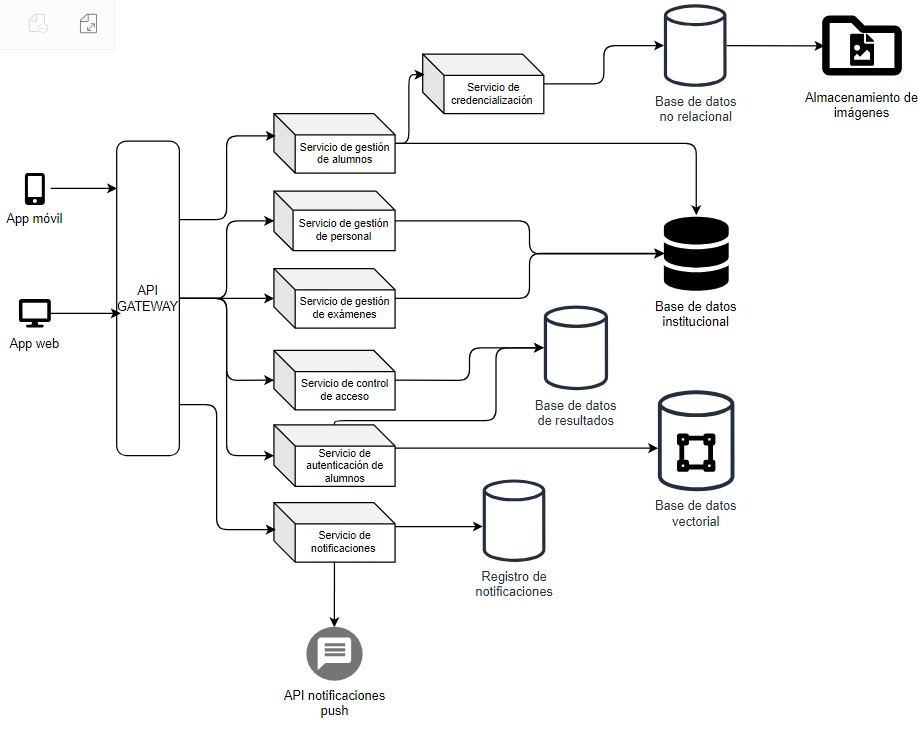
\includegraphics[width=.6\textwidth]{images/arquitectura}}
		\caption{Arquitectura del sistema.}
		\label{fig:arquitectura}
	\end{center}
\end{figure}

En la figura~\ref{fig:arquitectura} se describe la arquitectura general del sistema en la que se destaca el uso de un enfoque basado en micro-servicios, identificando los principales servicios que conforman la propuesta de solución y sus componentes principales.


%=========================================================
\section{Modelo del Negocio}	
\label{cap:reqSist}

	En está sección se modela la {\em Arquitectura del negocio} la cual está conformada por la Ontología del negocio ({\em Términos} y {\em Hechos del negocio}), Arquitectura de procesos y las {\em Reglas del negocio}. Primero se especifica brevemente el {\em Contexto} en el que los términos tienen significado.
		
	En las sección \ref{sec:terminosDeNegocio} se presentan los Términos del negocio a manera de Glosario y por último se presentan los Hechos del negocio a manera de relaciones entre términos del negocio.


%----------------------------------------------------------
\subsection{Contexto}

	El presente documento se desarrolla en el ámbito escolar dentro de una \hyperlink{tUnidadAcademica}{unidad académica}, en este caso, ESCOM (Escuela Superior de Cómputo). Dentro de esta \hyperlink{tUnidadAcademica}{unidad académica}, existen diferentes actores, como lo son, el \hyperlink{tPersonalSeguridad}{personal de seguridad}, el \hyperlink{tAlumno}{alumnado} y el \hyperlink{tPersonalAcademico}{personal académico}. Juntos desempeñan diferentes tareas que tienen que ver con el ámbito escolar, en este contexto, nos vamos a enfocar al proceso de ingreso del \hyperlink{tAlumno}{alumnado} a la \hyperlink{tUnidadAcademica}{unidad académica} durante el periodo de \hyperlink{tETS}{ETS}.
	
	El proceso que se lleva hasta ahora para poder realizar un \hyperlink{tETS}{ETS} es a través de la página escolar (\hyperlink{tSAES}{SAES}) de la \hyperlink{tUnidadAcademica}{unidad académica} a la que el \hyperlink{tAlumno}{alumno} pertenece. Una vez hecho esto, el \hyperlink{tAlumno}{alumno} debe de esperar al día de aplicación del \hyperlink{tETS}{ETS}, para poder presentarse a realizar el mismo.
	
	Actualmente, el \hyperlink{tAlumno}{alumnado} puede entrar a la \hyperlink{tUnidadAcademica}{unidad académica} mayormente sin alguna prueba de que van a realizar un \hyperlink{tETS}{ETS}, y ya en el salón de aplicación del \hyperlink{tETS}{ETS} les piden la credencial para saber si son quien dicen ser. Sin embargo, este proceso depende de cada docente, por lo que puede llegar a fallar y también, es muy propenso al fallo humano.
	
	Por esto, se propone un sistema que ayude a realizar el proceso de ingreso a la \hyperlink{tUnidadAcademica}{unidad académica}, por medio de un  \hyperlink{tControlAcceso}{control de acceso} que se apoye con un \hyperlink{tSistemaVerificacion}{Sistema de verificación de identidad}, o bien por medio del escanéo del \hyperlink{tCodigoQR}{código QR} que tiene la \hyperlink{tCredencialEscolar}{credencial escolar} en la parte trasera de la misma. 
	
%---------------------------------------------------------
\subsection{Términos del Negocio}
\label{sec:terminosDeNegocio}

\begin{description}
	% Ejemplo de un término literal.
	 \item[\hypertarget{tUnidadAcademica}{Unidad académica:}] Se refiere a la institución educativa en donde los usuarios se desenvuelven diariamente.
	
	\item[\hypertarget{tUnidadAprendizaje}{Unidad de aprendizaje:}] Son los elementos que componen un plan de estudios de alguna de las carreras ofertadas en la \hyperlink{tUnidadAcademica}{unidad académica}. Es necesario que los alumnos acrediten todas sus materias para continuar con su formación académica.
	
	\item[\hypertarget{tETS}{Exámen a Título de Suficiencia (ETS):}] Prueba final que permite a los alumnos acreditar una materia reprobada, y para la cual se requiere verificación de identidad.
	
	\item[\hypertarget{tAlumno}{Alumno:}] (es un tipo de Usuario) Se refiere a las personas inscritas dentro de algún plan de estudios ofertado en la \hyperlink{tUnidadAcademica}{unidad académica}.
	
	\item[\hypertarget{tPersonalAcademico}{Personal Académico:}] (es un tipo de Usuario) Se refiere a las personas registradas como trabajadores dentro de una unidad académica. Estos elaboran diferentes tipos de tareas dependiendo del rol o del cargo que tengan.
	
	\item[\hypertarget{tPersonalSeguridad}{Personal de seguridad:}] (es un tipo de Usuario) Se refiere a las personas registradas como trabajadores y que permiten o no el acceso a la \hyperlink{tUnidadAcademica}{unidad académica}.
	
	\item[\hypertarget{tCodigoQR}{Código QR:}] Código único generado por el sistema que permite resolver tareas de control de acceso a las instalaciones y a servicios de autenticación.
	
	\item[\hypertarget{tSistemaVerificacion}{Sistema de verificación de la identidad:}] Conjunto de procesos que permiten validar la identidad de los alumnos que buscan aplicar un ETS.
	
	\item[\hypertarget{tCredencialEscolar}{Credencial escolar:}] Documento con datos de identificación que pueden usarse junto a los registros de inscripción a ETS para permitir o no el acceso a la \hyperlink{tUnidadAcademica}{unidad académica}.
	
	\item[\hypertarget{tControlAcceso}{Control de acceso:}] Sistema implementado para verificar y autorizar el acceso a la \hyperlink{tUnidadAcademica}{unidad académica}.
	
	\item[\hypertarget{tRegistroAcceso}{Registro de acceso:}] Historial digital que documenta los accesos permitidos y denegados, incluyendo datos de cada intento de entrada para consulta posterior.
	
	\item[\hypertarget{tSAES}{SAES:}] Herramienta informática que utiliza el Instituto Politécnico Nacional (IPN) para pode controlar toda la información académica de cada estudiante.
	
%	\brTermSensor{tVelocimetro}{Velocímetro:}{Velocidad de un Vehículo.}{Kilometros/hora.}{Constantemente siempre que el \cdtRef{tVehiculo}{vehículo} esté encendido.}
\end{description}
%---------------------------------------------------------


\subsection{Modelo del dominio del problema}
\label{sec:modeloDeDominioP}

El modelo del dominio del problema se muestra en la figura~\ref{fig:modeloDeDominio}, a continuación se describen cada una de las entidades.

\newpage

\begin{figure}[htbp!]
	\begin{center}
		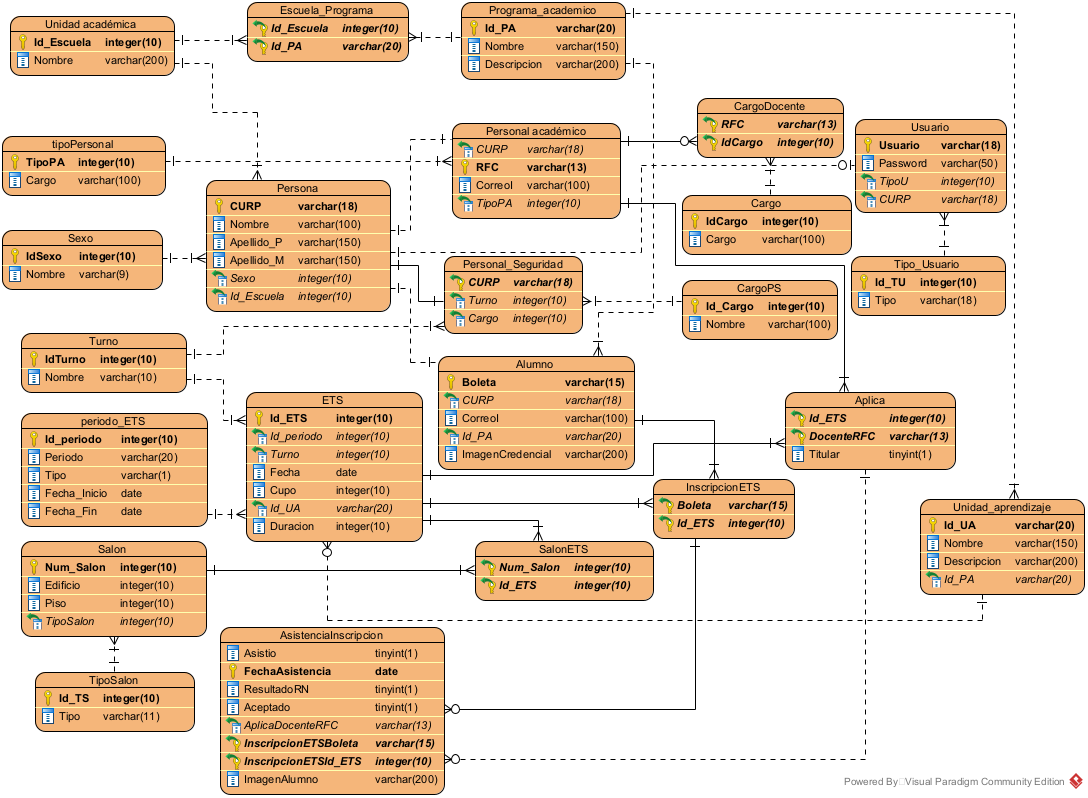
\includegraphics[angle=90,width=.80\textwidth]{images/DER}
		\caption{Modelo del dominio del problema}
		\label{fig:modeloDeDominio}
	\end{center}
\end{figure}

%---------------------------------------------------------
\begin{cdtEntidad}{Unidad academica}{Unidad academica}
	\brAttr{Id\_escuela}{Id\_escuela}{integer}{Número de registro usado para identificar a la escuela.}{Sí}
	\brAttr{nombre}{Nombre}{varchar}
	{Nombre de la escuela}{Sí}
%	\brAttr{ubicacion}{Ubicación}{Frase}
%	{Ubicación en la que se encuentra la escuela.}{Sí}
%	\brAttr{telefono}{Teléfono}{Teléfono}
%	{Teléfono para contactar a la escuela.}{Si}
%- - - - - - - - - - - - - - - - - - - - - - - - - - - - - 
	% \brRelComposition \brRelAgregation
%	\cdtEntityRelSection
%	\brRel{}{Programa\_académico}{ \hyperlink{Unidad academica}{Unidad académica} está compuesto por un \hyperlink{PA}{Programa académico}}	
%	\brRel{}{Persona}{Una \hyperlink{Persona}{Persona} pertenece a \hyperlink{Unidad academica}{Unidad academica}}	
\end{cdtEntidad}
%---------------------------------------------------------
\begin{cdtEntidad}{EscuelaPrograma}{Escuela\_Programa}
	\brAttr{Id\_Escuela}{Id\_Escuela}{integer}{Número de registro usado para identificar a la escuela.}{Sí}
	\brAttr{Id\_PA}{Id\_PA}{varchar}
	{Identificación del programa académico que imparte la Unidad académica.}{Sí}
\end{cdtEntidad}
%---------------------------------------------------------
\begin{cdtEntidad}{PA}{Programa\_academico}
	\brAttr{Id\_PA}{Id\_PA}{varchar}{Número de registro usado para identificar al programa académico.}{Sí}
	\brAttr{nombre}{Nombre}{varchar}
	{Nombre del programa académico}{Sí}
	\brAttr{descripcion}{Descripción}{varchar}
	{Descripción que habla sobre el programa académico.}{Sí}
%- - - - - - - - - - - - - - - - - - - - - - - - - - - - -
%	\cdtEntityRelSection
%	\brRel{}{Unidad\_aprendizaje}{Un \hyperlink{PA}{Programa academico} está compuesto por una \hyperlink{UA}{Unidad de aprendizaje}}	
%	\brRel{}{Unidad academica}{Una \hyperlink{Unidad academica}{Unidad academica} está compuesta por un \hyperlink{PA}{Programa académico}}	
\end{cdtEntidad}
%---------------------------------------------------------
\begin{cdtEntidad}{Persona}{Persona}
	\brAttr{CURP}{CURP}{Id}{Código usado para identificar a las personas.}{Sí}
	\brAttr{nombre}{Nombre}{varchar}
	{Nombre(s) de la persona.}{Sí}
	\brAttr{ApellidoP}{Apellido\_P}{varchar}
	{Apellido paterno de la persona.}{Sí}
	\brAttr{ApellidoM}{Apellido\_M}{varchar}
	{Apellido materno de la persona.}{Sí}
	\brAttr{sexo}{Sexo}{integer}
	{Letra que servirá para identificar el sexo de un alumno ('M' para masculino, 'F' para femenino).}{Sí}
	\brAttr{Id\_escuela}{Id\_escuela}{integer}
	{Id de la escuela a la que pertenece la persona.}{Si}
	%- - - - - - - - - - - - - - - - - - - - - - - - - - - - -
%	\cdtEntityRelSection
%	\brRel{}{Unidad academica}{Una \hyperlink{Persona}{Persona} pertenece a una \hyperlink{Unidad academica}{Unidad academica}}	
%	\brRel{}{Docente}{Una \hyperlink{Persona}{Persona} es un \hyperlink{Docente}{Docente}}	
%	\brRel{}{Personal\_Seguridad}{Una \hyperlink{Persona}{Persona} es un \hyperlink{PS}{Personal de seguridad}}
%	\brRel{}{Alumno}{Una \hyperlink{Persona}{Persona} es un  \hyperlink{Alumno}{Alumno}}
%	\brRel{}{Usuario}{Una \hyperlink{Persona}{Persona} cuenta con un \hyperlink{Usuario}{Usuario}}
\end{cdtEntidad}
%---------------------------------------------------------
\begin{cdtEntidad}{PersonalAcademico}{Personal académico}
	\brAttr{CURP}{CURP}{varchar}{Código usado para identificar a las personas.}{Sí}
	\brAttr{RFC}{RFC}{varchar}
	{RFC que identifica al personal académico.}{Sí}
	\brAttr{CorreoI}{CorreoI}{varchar}
	{Correo institucional del personal académico.}{Sí}
	\brAttr{TipoPA}{TipoPA}{integer}{Número que identifica que tipo de personal académico es, ya sea, por ejemplo, un docente o personal de gestión escolar.}{Sí}
	%- - - - - - - - - - - - - - - - - - - - - - - - - - - - -
%	\cdtEntityRelSection
%	\brRel{}{CargoDocente}{Un \hyperlink{PersonalAcademico}{personal académico} puede ser un \hyperlink{CargoDocente}{Docente}}
%	\brRel{}{ETS}{Un \hyperlink{PersonalAcademico}{Docente} \hyperlink{Aplica}{Aplica} un \hyperlink{ETS}{ETS}}
%	\brRel{}{Persona}{Un \hyperlink{PersonalAcademico}{personal académico} es una \hyperlink{Persona}{Persona}}
%	\brRel{}{tipoPersonal}{Un \hyperlink{PersonalAcademico}{personal académico} tiene asignado un \hyperlink{Cargo}{Cargo}}
\end{cdtEntidad}
%---------------------------------------------------------
\begin{cdtEntidad}{tipoPA}{tipoPersonal}
	\brAttr{TipoPA}{TipoPA}{integer}
	{Número que identifica que tipo de personal académico es la persona.}{Sí}
	\brAttr{Cargo}{Cargo}{varchar}{Nombre del tipo de personal académico que tendrá la persona.}{Sí}
\end{cdtEntidad}
%---------------------------------------------------------
\begin{cdtEntidad}{CargoDocente}{CargoDocente}
	\brAttr{RFC}{RFC}{varchar}
	{RFC que identifica al Docente.}{Sí}
	\brAttr{IdCargo}{IdCargo}{integer}{Código usado para identificar un cargo dentro de la escuela.}{Sí}
\end{cdtEntidad}
%---------------------------------------------------------
\begin{cdtEntidad}{Cargo}{Cargo}
	\brAttr{IdCargo}{IdCargo}{integer}{Código usado para identificar un cargo dentro de la escuela.}{Sí}
	\brAttr{Cargo}{Cargo}{varchar}
	{Nombre del cargo existente dentro de la institución escolar.}{Sí}
	%- - - - - - - - - - - - - - - - - - - - - - - - - - - - -
%	\cdtEntityRelSection
%	\brRel{}{CargoDocente}{Un \hyperlink{Cargo}{Cargo} es asignado a un \hyperlink{PersonalAcademico}{Docente}}
\end{cdtEntidad}
%---------------------------------------------------------
\begin{cdtEntidad}{PS}{Personal\_Seguridad}
	\brAttr{rfc}{RFC}{varchar}{Código usado para identificar a un personal de seguridad}{Sí.}
	\brAttr{CURP}{CURP}{varchar}{CURP de la persona.}{Sí}
	\brAttr{Turno}{Turno}{integer}
	{Letra usada identificar el turno en el que se aplica el ETS ('M' para matutino, 'V' para vespertino).}{Sí}
	\brAttr{Cargo}{Cargo}{integer}
	{Nombre del cargo del personal de seguridad.}{Sí}
	%- - - - - - - - - - - - - - - - - - - - - - - - - - - - -
%	\cdtEntityRelSection
%	\brRel{}{Persona}{Un \hyperlink{PS}{Personal de seguridad} es una \hyperlink{Persona}{Persona}}
\end{cdtEntidad}
%---------------------------------------------------------
\begin{cdtEntidad}{CargoPS}{CargoPS}
	\brAttr{Id\_Cargo}{Id\_Cargo}{integer}{Código usado para identificar el cargo que tiene el personal de seguridad.}{Sí}
	\brAttr{Cargo}{Cargo}{varchar}
	{Nombre del cargo del personal de seguridad.}{Sí}
\end{cdtEntidad}
%---------------------------------------------------------
\begin{cdtEntidad}{Alumno}{Alumno}
	\brAttr{Boleta}{Boleta}{varchar}
	{Código usado para identificar al alumnado de la institución}{Sí}
	\brAttr{CURP}{CURP}{varchar}{Código usado para identificar a las personas.}{Sí}
	\brAttr{CorreoI}{CorreoI}{varchar}
	{Correo institucional del alumno.}{Sí}
	\brAttr{Id\_PA}{Id\_PA}{varchar}
	{Identificación del programa académico al que pertenece el alumno.}{Sí}
	\brAttr{ImagenCredencial}{ImagenCredencial}{varchar}
	{Ruta de donde está guardada la imagen de la credencial del alumno.}{Sí}
	%- - - - - - - - - - - - - - - - - - - - - - - - - - - - -
%	\cdtEntityRelSection
%	\brRel{}{Persona}{Un \hyperlink{Alumno}{Alumno} es una \hyperlink{Persona}{Persona}}
%	\brRel{}{ETS}{Un \hyperlink{Alumno}{Alumno} tiene una \hyperlink{InscripcionETS}{inscripción} a un \hyperlink{ETS}{ETS}}
\end{cdtEntidad}
%---------------------------------------------------------
\begin{cdtEntidad}{Usuario}{Usuario}
	\brAttr{Usuario}{Usuario}{varchar}{Nombre de usuario asignado a una persona dentro del sistema.}{Sí}
	\brAttr{Password}{Password}{varchar}
	{Contraseña ligada al usuario de una persona registrada dentro del sistema.}{Sí}
	\brAttr{TipoU}{TipoU}{integer}
	{Número que identificará a los tipos de usuario registrados dentro del sistema.}{Sí}
	\brAttr{CURP}{CURP}{varchar}
	{Código usado para identificar a las personas.}{Sí}
	%- - - - - - - - - - - - - - - - - - - - - - - - - - - - -
%	\cdtEntityRelSection
%	\brRel{}{Persona}{Un \hyperlink{Usuario}{Usuario} es asignado a una \hyperlink{Persona}{Persona}}
%	\brRel{}{Tipo\_Usuario}{Un \hyperlink{Usuario}{Usuario} tiene un \hyperlink{TU}{Tipo de usuario}}
\end{cdtEntidad}
%---------------------------------------------------------
\begin{cdtEntidad}{TU}{Tipo\_Usuario}
	\brAttr{Id\_TU}{Id\_TU}{integer}
	{RFC que identifica al personal académico.}{Sí}
	\brAttr{Tipo}{Tipo}{varchar}{Frase que definirá el tipo de usuario que tienen las personas.}{Sí}
\end{cdtEntidad}
%---------------------------------------------------------
\begin{cdtEntidad}{ETS}{ETS}
	\brAttr{Id\_ETS}{Id\_ETS}{integer}{Número usado para identificar los diferentes ETS registrados.}{Sí}
	\brAttr{Id\_periodo}{Id\_periodo}{integer}
	{Número usado para identificar el periodo en el que se realiza el ETS.}{Sí}
	\brAttr{Turno}{Turno}{integer}
	{Letra usada identificar el turno en el que se aplica el ETS ('M' para matutino, 'V' para vespertino).}{Sí}
	\brAttr{Fecha}{Fecha}{datetime}
	{Fecha y hora en la que se realizará el ETS.}{Sí}
	\brAttr{Cupo}{Cupo}{integer}
	{Número de personas permitidas a realizar el ETS.}{Sí}
	\brAttr{Id\_UA}{Id\_UA}{varchar}
	{Identificación de la Unidad de aprendizaje del ETS.}{Sí}
	\brAttr{Duracion}{Duracion}{integer}
	{Duración en horas del ETS.}{Sí}
	\brAttr{Hora}{Hora}{time}
	{Duración en horas del ETS.}{Sí}
	%- - - - - - - - - - - - - - - - - - - - - - - - - - - - -
%	\cdtEntityRelSection
%	\brRel{}{periodo\_ETS}{Un \hyperlink{ETS}{ETS} se realiza un en \hyperlink{PETS}{periodo}}
%	\brRel{}{Alumno}{En un \hyperlink{ETS}{ETS} está \hyperlink{InscripcionETS}{inscrito} un \hyperlink{Alumno}{Alumno}}
%	\brRel{}{Personal academico}{Un \hyperlink{ETS}{ETS} es \hyperlink{Aplica}{aplicado} por un \hyperlink{PersonalAcademico}{Docente}}
%	\brRel{}{Salon}{A un \hyperlink{ETS}{ETS} le \hyperlink{SalonETS}{corresponde} un \hyperlink{Salon}{Salón}}
%	\brRel{}{Unidad\_Aprendizaje}{Un \hyperlink{ETS}{ETS} \hyperlink{ETSUA}{es de} una \hyperlink{UA}{Unidad de Aprendizaje}.}
\end{cdtEntidad}
%---------------------------------------------------------
\begin{cdtEntidad}{PETS}{periodo\_ETS}
	\brAttr{Id\_periodo}{Id\_periodo}{integer}{Número usado para identificar el periodo en el que se realizarán los ETS registrados.}{Sí}
	\brAttr{Periodo}{Periodo}{varchar}
	{Periodo registrado en el que se realizarán los ETS.}{Sí}
	\brAttr{Tipo}{Tipo}{varchar}
	{Letra usada identificar el tipo de los ETS que se aplicarán ('O' para ordinario, 'E' para especial).}{Sí}
	\brAttr{Fecha\_Inicio}{Fecha\_Inicio}{date}
	{Fecha en la que iniciará el periodo de los ETS.}{Sí}
	\brAttr{Fecha\_Fin}{Fecha\_Fin}{date}
	{Fecha en la que terminará el periodo de los ETS.}{Sí}
	%- - - - - - - - - - - - - - - - - - - - - - - - - - - - -
%	\cdtEntityRelSection
%	\brRel{}{ETS}{En un \hyperlink{PETS}{periodo de ETS} se realizan los \hyperlink{ETS}{ETS}.}
\end{cdtEntidad}
%---------------------------------------------------------
\begin{cdtEntidad}{Aplica}{Aplica}
	\brAttr{Id\_ETS}{Id\_ETS}{integer}{Número usado para identificar los diferentes ETS registrados.}{Sí}
	\brAttr{DocenteRFC}{DocenteRFC}{varchar}
	{RFC que identifica al Docente.}{Sí}
	\brAttr{Titular}{Coordinador}{tinyint}
	{Booleano que identificará si el profesor que aplicará el ETS es el titular o es un ayudante.}{Sí}
\end{cdtEntidad}
%---------------------------------------------------------
\begin{cdtEntidad}{InscripcionETS}{InscripcionETS}
	\brAttr{Boleta}{Boleta}{varchar}
	{Código usado para identificar al alumnado de la institución}{Sí}
	\brAttr{Id\_ETS}{Id\_ETS}{integer}{Número usado para identificar los diferentes ETS registrados.}{Sí}
\end{cdtEntidad}
%---------------------------------------------------------
\begin{cdtEntidad}{SalonETS}{SalonETS}
	\brAttr{Num\_Salon}{Num\_Salon}{integer}
	{Número usado para identificar al salón en el que se aplicará un ETS.}{Sí}
	\brAttr{Id\_ETS}{Id\_ETS}{integer}{Número usado para identificar los diferentes ETS registrados.}{Sí}
\end{cdtEntidad}
%---------------------------------------------------------
\begin{cdtEntidad}{Salon}{Salon}
	\brAttr{Num\_Salon}{Num\_Salon}{integer}
	{Número usado para identificar el salón en el que se aplicará un ETS.}{Sí}
	\brAttr{Edificio}{Edificio}{integer}
	{Número usado para identificar el edificio en el que se realizará el ETS.}{Sí}
	\brAttr{Piso}{Piso}{integer}
	{Número usado para identificar el piso del edificio en el que se realizará el ETS.}{Sí}
	\brAttr{TipoSalon}{integer}{Id}
	{Identificación del tipo de salón en el que se va a aplicar el ETS.}{Sí}
	%- - - - - - - - - - - - - - - - - - - - - - - - - - - - -
%	\cdtEntityRelSection
%	\brRel{}{ETS}{Un \hyperlink{Salon}{Salon} es \hyperlink{SalonETS}{ocupado} para llevar a cabo un \hyperlink{ETS}{ETS}.}
\end{cdtEntidad}
%---------------------------------------------------------
\begin{cdtEntidad}{TipoSalon}{TipoSalon}
	\brAttr{Num\_Salon}{Num\_Salon}{integer}
	{Número usado para identificar el salón en el que se aplicará un ETS.}{Sí}
	\brAttr{Tipo}{Tipo}{varchar}
	{Frase indicando el tipo de salón en el que se aplicará el ETS.}{Sí}
	%- - - - - - - - - - - - - - - - - - - - - - - - - - - - -
	%	\cdtEntityRelSection
	%	\brRel{}{ETS}{Un \hyperlink{Salon}{Salon} es \hyperlink{SalonETS}{ocupado} para llevar a cabo un \hyperlink{ETS}{ETS}.}
\end{cdtEntidad}
%---------------------------------------------------------
\begin{cdtEntidad}{UA}{Unidad\_aprendizaje}
	\brAttr{Id\_UA}{Id\_UA}{varchar}
	{Identificación de la Unidad de Aprendizaje.}{Sí}
	\brAttr{Nombre}{Nombre}{varchar}
	{Nombre de la unidad de aprendizaje.}{Sí}
	\brAttr{Descripcion}{Descripcion}{varchar}
	{Descripción pequeña de lo que trata la unidad de aprendizaje.}{Sí}
	\brAttr{Id\_PA}{Id\_PA}{varchar}
	{Identificación del programa académico al que pertenece la unidad de aprendizaje.}{Sí}
	%- - - - - - - - - - - - - - - - - - - - - - - - - - - - -
%	\cdtEntityRelSection
%	\brRel{}{ETS}{A una \hyperlink{UA}{Unidad de aprendizaje} le \hyperlink{ETSUA}{corresponde} una serie de \hyperlink{ETS}{ETS}.}
\end{cdtEntidad}
%---------------------------------------------------------
\begin{cdtEntidad}{Turno}{Turno}
	\brAttr{IdTurno}{IdTurno}{integer}
	{Identificación del turno.}{Sí}
	\brAttr{Nombre}{Nombre}{varchar}
	{Nombre del turno. Este puede variar entre 'Matutino' y 'Vespertino'.}{Sí}
\end{cdtEntidad}
%---------------------------------------------------------
\begin{cdtEntidad}{Sexo}{Sexo}
	\brAttr{IdSexo}{IdSexo}{integer}
	{Identificación del sexo.}{Sí}
	\brAttr{Nombre}{Nombre}{varchar}
	{Nombre del sexo. Este puede variar entre 'Masculino' y 'Femenino'.}{Sí}
\end{cdtEntidad}
%---------------------------------------------------------
\begin{cdtEntidad}{IngresoInstalacion}{ingreso\_instalacion}
	\brAttr{boleta}{Boleta}{varchar}
	{Código usado para identificar al alumnado de la institución una vez que entre a las instalaciones de la escuela.}{Sí}
	\brAttr{idets}{Id\_ETS}{integer}
	{ETS que el alumno realizará.}{Sí}
	\brAttr{fecha}{fecha}{date}
	{Fecha en la que el alumno se presenta a las instalaciones.}{Sí}
	\brAttr{hora}{hora}{time}
	{Hora en la que el alumno ingresa a las instalaciones.}{Sí}
\end{cdtEntidad}
%---------------------------------------------------------
\begin{cdtEntidad}{tipoEstado}{tipo\_estado}
	\brAttr{idtipo}{idtipo}{integer}
	{Número que identifica los distintos tipos de estatus de la asistencia del alumno.}{Sí}
	\brAttr{tipo}{tipo}{varchar}
	{Estatus que define el resultado de la operación del registro de asistencia del alumno a su ETS.}{Sí}
\end{cdtEntidad}
%---------------------------------------------------------
\begin{cdtEntidad}{ingresoSalon}{ingreso\_salon}
	\brAttr{boleta}{Boleta}{varchar}
	{Código usado para identificar al alumnado de la institución una vez que ingrese al salón en donde se aplicará su ETS.}{Sí}
	\brAttr{idets}{idets}{integer}
	{ETS al que el alumno se presenta.}{Sí}
	\brAttr{fecha}{fecha}{date}
	{Fecha en la que el alumno se presenta a realizar su ETS.}{Sí}
	\brAttr{hora}{hora}{time}
	{Hora en la que el alumno ingresa al salón en el que realizará el ETS.}{Sí}
	\brAttr{docente}{docente}{varchar}
	{Docente que realiza el pase de asistencia del alumno.}{Sí}
	\brAttr{estado}{estado}{integer}
	{Registro que indica si al alumno le permitieron o no realizar el ETS.}{Sí}
\end{cdtEntidad}
%---------------------------------------------------------
\begin{cdtEntidad}{motivorechazo}{motivo\_rechazo}
	\brAttr{boleta}{Boleta}{varchar}
	{Código usado para identificar al alumnado.}{Sí}
	\brAttr{idets}{idets}{integer}
	{ETS al que el alumno se presenta a realizar.}{Sí}
	\brAttr{motivo}{motivo}{varchar}
	{Motivo por el cual al alumno no se le permitió realizar su ETS.}{Sí}
\end{cdtEntidad}
%---------------------------------------------------------
\begin{cdtEntidad}{resultadorn}{resultadorn}
	\brAttr{boleta}{Boleta}{varchar}
	{Código usado para identificar al alumnado.}{Sí}
	\brAttr{idets}{idets}{integer}
	{ETS al que el alumno se presenta a realizar.}{Sí}
	\brAttr{precision}{precision}{varchar}
	{Precisión que obtuvo el modelo de reconocimiento facial con la imagen que se le tomó al alumno.}{Sí}
	\brAttr{imagenAlumno}{imagen\_alumno}{varchar}
	{Ruta donde está guardada la imagen que se le tomó al alumno al momento de realizar el reconocimiento facial.}{Sí}
\end{cdtEntidad}
%---------------------------------------------------------
\begin{cdtEntidad}{tokenNotificacion}{token\_notificacion}
	\brAttr{id}{id}{integer}
	{Número con el que se identifica el token de un usuario al ingresar en la app.}{Sí}
	\brAttr{usuario}{usuario}{varchar}
	{Usuario de alguna de las personas registradas en la app.}{Sí}
	\brAttr{token}{token}{varchar}
	{Token usado para identificar a un usuario.}{Sí}
\end{cdtEntidad}
%---------------------------------------------------------
\begin{cdtEntidad}{chat}{chat}
	\brAttr{id}{id}{integer}
	{Número con el que se identifica el chat entre dos usuarios.}{Sí}
	\brAttr{remitente}{remitente}{varchar}
	{Usuario que inició el chat.}{Sí}
	\brAttr{destinatario}{destinatario}{varchar}
	{Segundo usuario que participa en el chat.}{Sí}
\end{cdtEntidad}
%---------------------------------------------------------
\begin{cdtEntidad}{mensaje}{mensaje}
	\brAttr{chat}{chat}{integer}
	{Número con el que se identifica el chat entre dos usuarios.}{Sí}
	\brAttr{fecha}{fecha}{datetime}
	{Fecha y hora en la que un mensaje se envió.}{Sí}
	\brAttr{remitente}{remitente}{varchar}
	{Usuario que envía el mensaje.}{Sí}
	\brAttr{mensaje}{mensaje}{varchar}
	{Mensaje que envía un usuario.}{Sí}
\end{cdtEntidad}
%---------------------------------------------------------
\subsection{Modelado de Reglas de negocio}

\begin{BussinesRule}{RN1}{Acceso al sistema.}
	\BRitem[Tipo:] Acceso. 
	\BRitem[Clase:] Condicional. 
	\BRitem[Nivel:] Estricto.
	\BRitem[Descripción:] El acceso a nuestro sistema será permitido solo para los Empleados y estudiantes de la ESCOM.
	\BRitem[Motivación:] Evitar el acceso no autorizado a otras personas que no sean de la ESCOM..

	\BRitem[Referenciado por:] \hyperlink{CU-01}{CU-01} y \hyperlink{CU41}{CU-41}.
\end{BussinesRule}

\begin{BussinesRule}{RN2}{ Acceso a las funcionalidades del docente.}
    \BRitem[Tipo:] Acceso. 
    \BRitem[Clase:] Condicional. 
    \BRitem[Nivel:] Estricto.
    \BRitem[Descripción:] Los docentes solo podrán acceder y revisar la información de los ETS que tengan asignados.
    \BRitem[Motivación:] Para evitar que los docentes se confundan, accedan a información que no les corresponde o modifiquen información que no les corresponde.

    \BRitem[Referenciado por:] \hyperlink{CU-01}{CU-01} y \hyperlink{CU-04}{CU-04}.
\end{BussinesRule}

\begin{BussinesRule}{RN3}{ Acceso a las funcionalidades del personal de seguridad.}
    \BRitem[Tipo:] Acceso. 
    \BRitem[Clase:] Condicional. 
    \BRitem[Nivel:] Estricto.
    \BRitem[Descripción:] El personal de seguridad solo podrán acceder y revisar la información relacionada con el acceso de los alumnos a la ESCOM de los días en los que se presenten ETS.
    \BRitem[Motivación:] Para evitar que el personal de seguridad se confunda, accedan a información que no les corresponde o modifiquen información que no les corresponde.

    \BRitem[Referenciado por:] \hyperlink{CU-01}{CU-01} y \hyperlink{CU-12}{CU-12}, \hyperlink{CU-13}{CU-13}, \hyperlink{CU-14}{CU-14} y \hyperlink{CU-15}{CU-15}.
\end{BussinesRule}

\begin{BussinesRule}{RN4}{ Acceso a las funcionalidades web}
	\BRitem[Tipo:] Habilitación.
	\BRitem[Clase:] Condicional.
	\BRitem[Nivel:] Estricta.
	\BRitem[Descripción:] El sistema permitirá únicamente a el personal de gestión escolar y al personal la DAE acceder al sistema web.
	\BRitem[Motivación:] Se necesita separar las funcionalidades de los empleados para que el sistema tenga cohesión y para que el sistema web no referencie al sistema movil.
	\BRitem[Referenciado por:] \hyperlink{CU-41}{CU-41}.
	\end{BussinesRule}

\begin{BussinesRule}{RN5} {Consultar periodos del docente}
	\BRitem[Tipo:] Habilitación.
	\BRitem[Clase:] Condicional.
	\BRitem[Nivel:] Estricta.
	\BRitem[Descripción:] El sistema permitirá únicamente a los docentes autenticados consultar los períodos de ETS que tiene asignados.
	\BRitem[Motivación:] Garantizar que solo usuarios autorizados consulten información sensible.			
	\BRitem[Referenciado por:] \hyperlink{CU-04}{CU-04}.
	\end{BussinesRule}

\begin{BussinesRule}{RN6} {Visualizar lista de alumnos inscritos}
	\BRitem[Tipo:] Acceso.
	\BRitem[Clase:] Condicional.
	\BRitem[Nivel:] Estricta.
	\BRitem[Descripción:] El sistema permitirá al docente consultar únicamente la lista de los alumnos inscritos a los ETS que le han sido asignados.
	\BRitem[Motivación:] Permitir que los docentes puedan visualizar la información de los estudiantes inscritos a los ETS que tenga asignados.
	\BRitem[Referenciado por:] \hyperlink{CU-09}{CU-09}.
	\end{BussinesRule}

\begin{BussinesRule}{RN7} {Acceso al asignar remplazo}
    \BRitem[Tipo:] Acceso.
    \BRitem[Clase:] Condicional.
    \BRitem[Nivel:] Estricta.
    \BRitem[Descripción:] El sistema permitirá solo al presidente de academia  y al jefe de departamento consultar la lista de solicitudes de remplazo y posteriormente asignar un remplazo.
    \BRitem[Motivación:] Hacer que solo el personal capacitado y responsable asigne los remplazos a los ETS.
    \BRitem[Referenciado por:] \hyperlink{CU-42}{CU-42}.
    \end{BussinesRule}

\begin{BussinesRule}{RN8} {Cantidad de pruebas de reconocimiento facial}
    \BRitem[Tipo:]Habilitación.
    \BRitem[Clase:]Cronometrada.
    \BRitem[Nivel:] Estricta.
    \BRitem[Descripción:] El alumno solo puede realizar un máximo de 3 pruebas de reconocimiento facial dentro de la aplicación.
    \BRitem[Motivación:] Evitar que el alumno le pida a alguien más que  pruebe constantemente el reconocimiento facial hasta que se parezca a el/ella.
    \BRitem[Referenciado por:] \hyperlink{CU-19}{CU-19}.
    \end{BussinesRule}

\begin{BussinesRule}{RN9} {Cantidad de intentos fallidos de inicio de sesión}
    \BRitem[Tipo:]Habilitación.
    \BRitem[Clase:] Cronometrada.
    \BRitem[Nivel:] Estricta.
    \BRitem[Descripción:] El sistema permitirá solo a todos los usuarios un máximo de 5 intentos de inicio de sesión fallidos antes de bloquear la cuenta del usuario.
    \BRitem[Motivación:] Asegurar la seguridad de los usuarios y evitar que personas no autorizadas entren al sistema.
    \BRitem[Referenciado por:] \hyperlink{CU-01}{CU-01}, y \hyperlink{CU-41}{CU-41}.
    \end{BussinesRule}

\begin{BussinesRule}{RN10} {Acceso a solo la información de los ETS }
    \BRitem[Tipo:]Habilitadora.
    \BRitem[Clase:]Condicional.
    \BRitem[Nivel:] Estricta.
    \BRitem[Descripción:] El sistema permitirá que los alumnos puedan ingresar solo a la información de sus ETS inscritos y solo consultar a la información (no podrán modificarla).
    \BRitem[Motivación:] Evitar que los alumnos cambien la información de los ETS y evitar que los alumnos sepan de otros alumnos que presentaran el mismo ETS (esto para no fomentar la formación de acuerdos entre los alumnos).
    \BRitem[Referenciado por:] \hyperlink{CU-19}{CU-19}.
    \end{BussinesRule}

% Alfredo

\begin{BussinesRule}{BR11}{Registro de usuarios válidos.} 
    \BRitem[Tipo:] Habilitadora
    \BRitem[Clase:] Integridad
    \BRitem[Nivel:] Estricta
    \BRitem[Descripción:] Todos los usuarios registrados dentro del sistema deberán de estar registrados dentro de la tabla “Persona”. 
    \BRitem[Motivación:] Asegurar que solo la comunidad de la institución pueda acceder a la escuela. 
    \BRitem[Referenciado por:] \hyperlink{Usuario}{Usuario} 
    \end{BussinesRule}

\begin{BussinesRule}{BR12}{Registro de personal académico.} 
    \BRitem[Tipo:] Habilitadora
    \BRitem[Clase:] Condición.
    \BRitem[Nivel:] Estricta
    \BRitem[Descripción:] Para registrar al personal académico se deberá de dar de alta un RFC, un correo institucional válido y especificar el cargo que tiene dentro de la institución. Este puede variar entre un docente o personal administrativo, como lo es el personal de gestión escolar. En caso de ser un docente se debe especificar su cargo dentro de la escuela, como lo es el jefe de academia, presidente de academia, director o subdirector. 
    \BRitem[Motivación:] Moderar los diferentes permisos de los usuarios dependiendo del cargo que tengan dentro de la escuela. 
    \BRitem[Referenciado por:] \hyperlink{PersonalAcademico}{Personal Académico} 
    \end{BussinesRule}

\begin{BussinesRule}{BR13}{Límite de alumnos en un ETS.} 
    \BRitem[Tipo:] Cronometrada. 
    \BRitem[Clase:] Condición.
    \BRitem[Nivel:] Estricta
    \BRitem[Descripción:] Un alumno se podrá inscribir a un ETS únicamente si la cantidad de alumnos aún no excede el cupo límite de un ETS.
    \BRitem[Motivación:] Evitar el sobrecupo de un salón el día del ETS.
    \BRitem[Referenciado por:] \hyperlink{ETS}{ETS} 
    \end{BussinesRule}
    
\begin{BussinesRule}{BR14}{Fecha de aplicación de los ETS.} 
    \BRitem[Tipo:] Cronometrada. 
    \BRitem[Clase:] Condición.
    \BRitem[Nivel:] Estricta
    \BRitem[Descripción:] Las fechas de los ETS deben de estar dentro del periodo especificado del mismo, en caso contrario no se podrá dar de alta. 
    \BRitem[Motivación:] Tener un control sobre las fechas en las que se aplican los ETS. 
    \BRitem[Referenciado por:] \hyperlink{ETS}{ETS} 
    \end{BussinesRule}

\begin{BussinesRule}{BR15}{Registro de un ETS} 
    \BRitem[Tipo:] Habilitadora. 
    \BRitem[Clase:] Condición.
    \BRitem[Nivel:] Estricta
    \BRitem[Descripción:] Los ETS deberán de especificar siempre el turno en el ques e van a aplicar, especificar el periodo en el que se aplican y el cupo que se tendrá para ese ETS.
    \BRitem[Motivación:] Tener un mejor control sobre la información de los ETS.
    \BRitem[Referenciado por:] \hyperlink{ETS}{ETS} 
    \end{BussinesRule}

\begin{BussinesRule}{BR16}{Asignación de salón para un ETS} 
    \BRitem[Tipo:] Habilitadora. 
    \BRitem[Clase:] Condición	.
    \BRitem[Nivel:] Estricta
    \BRitem[Descripción:] Un salón solo puede ser asignado a un ETS si no ha sido asignado para otro ETS.
    \BRitem[Motivación:] Evitar la sobreasignación de salones.
    \BRitem[Referenciado por:] \hyperlink{SalonETS}{Salón del ETS} 
    \end{BussinesRule}

\begin{BussinesRule}{BR17}{Permisos del usuario de los docentes.} 
    \BRitem[Tipo:] Ejecutiva.
    \BRitem[Clase:] Autorización.
    \BRitem[Nivel:] Estricta
    \BRitem[Descripción:] Si un docente tiene asignado más de un cargo dentro de la institución, el sistema le mostrará las interfaces correspondientes a cada uno de los cargos. El acceso a las interfaces dependerá de las funcionalidades permitidas por cada cargo.
    \BRitem[Motivación:] Asegurar que los docentes tengan acceso a todas las funciones dependiendo del cargo que tengan.
    \BRitem[Referenciado por:] \hyperlink{CargoDocente}{Cargo del docente} 
    \end{BussinesRule}

\begin{BussinesRule}{BR18}{Número de docentes aplicadores de un ETS.} 
    \BRitem[Tipo:] Habilitadora. 
    \BRitem[Clase:] Condición.
    \BRitem[Nivel:] Estricta
    \BRitem[Descripción:] Un mismo ETS puede ser aplicado por múltiples docentes en diferentes salones.
    \BRitem[Motivación:] Asegurar que todos los ETS tengan por lo menos un aplicador, ya sea en uno o más salones.
    \BRitem[Referenciado por:] \hyperlink{Aplica}{Tabla Aplica} 
    \end{BussinesRule}

\begin{BussinesRule}{BR19}{Inscripción de un ETS.} 
    \BRitem[Tipo:] Habilitadora. 
    \BRitem[Clase:] Autorización.
    \BRitem[Nivel:] Estricta
    \BRitem[Descripción:] Un alumno no puede estar inscrito en dos ETS que se lleven a cabo en el mismo horario.
    \BRitem[Motivación:] Evitar el solapamiento de dos o más ETS.
    \BRitem[Referenciado por:] \hyperlink{InscripcionETS}{Inscripción de un ETS} 
    \end{BussinesRule}

\begin{BussinesRule}{BR20}{Aplicador titular de un ETS.} 
    \BRitem[Tipo:] Integridad
    \BRitem[Clase:] Cronometrada.
    \BRitem[Nivel:] Estricta
    \BRitem[Descripción:] Los ETS deberán contar siempre con un docente titular que es el docente principal que va a aplicar el ETS. En caso de sustitución del docente o apoyo a este, también se especificará que estos son ayudantes y no titulares.
    \BRitem[Motivación:] Garantizar la asignación de roles dentro del sistema.
    \BRitem[Referenciado por:] \hyperlink{Aplica}{Tabla Aplica} 
    \end{BussinesRule}
    

%
\begin{BussinesRule}{RN21} {Acceso a información sobre el acceso a los ETS}
    \BRitem[Tipo:] Acceso.
    \BRitem[Clase:]Condicional.
    \BRitem[Nivel:] Estricta.
    \BRitem[Descripción:] El sistema permitirá que solo los alumnos puedan acceder a la información sobre los ETS en una pantalla.
    \BRitem[Motivación:] Permitir que los alumnos conozcan el proceso de acceso a los ETS y evitar confusiones y malentendidos.
    \BRitem[Referenciado por:] \hyperlink{CU-20}{CU-20}.
    \end{BussinesRule}

\begin{BussinesRule}{RN22} {Estructura de la CURP}
    \BRitem[Tipo:]Integridad.
    \BRitem[Clase:]Condicional.
    \BRitem[Nivel:] Estricta.
    \BRitem[Descripción:] La CURP debe de tener exactamente 18 caracteres y debe de poseer solo letras y números.
    \BRitem[Motivación:] Para mantener la estructura correcta de la CURP y evitar que se Introduzca datos inválidos.
    \BRitem[Referenciado por:] \hyperlink{CU-21}{CU-21}, \hyperlink{CU-22}{CU-22}, \hyperlink{CU-33}{CU-33} y \hyperlink{CU-37}{CU-37}.
    \end{BussinesRule}

\begin{BussinesRule}{RN23} {Estructura de la Boleta}
    \BRitem[Tipo:]Integridad.
    \BRitem[Clase:]Condicional.
    \BRitem[Nivel:] Estricta.
    \BRitem[Descripción:] La Boleta debe de tener exactamente 10 caracteres y debe de poseer solo números.
    \BRitem[Motivación:] Para mantener la estructura correcta de la Boleta y evitar que se Introduzca datos inválidos.
    \BRitem[Referenciado por:] \hyperlink{CU-21}{CU-21}, \hyperlink{CU-22}{CU-22}, \hyperlink{CU-33}{CU-33} y \hyperlink{CU-37}{CU-37}.
    \end{BussinesRule}

\begin{BussinesRule}{RN24} {Estructura del correo institucional del alumno}
    \BRitem[Tipo:]Integridad.
    \BRitem[Clase:]Condicional.
    \BRitem[Nivel:] Estricta.
    \BRitem[Descripción:] El correo institucional del alumno debe de seguir la estructura [texto][@][alumno.ipn.mx]
    \BRitem[Motivación:] Para mantener la estructura correcta del correo institucional y evitar que se Introduzca datos inválidos.
    \BRitem[Referenciado por:] \hyperlink{CU-21}{CU-21} y \hyperlink{CU-22}{CU-22}.
    \end{BussinesRule}

\begin{BussinesRule}{RN25} {Cantidad de alumnos por salud}
    \BRitem[Tipo:] Habilitación.
    \BRitem[Clase:] Cronometrada.
    \BRitem[Nivel:] Estricta.
    \BRitem[Descripción:] Los salones tienen un cupo máximo de 30 alumnos.
    \BRitem[Motivación:] Para evitar aglomeraciones de alumnos durante un ETS.
    \BRitem[Referenciado por:] \hyperlink{CU-21}{CU-21} y \hyperlink{CU-22}{CU-22}.
    \end{BussinesRule}

\begin{BussinesRule}{RN26} {Asignación de salones}
    \BRitem[Tipo:] Habilitación.
    \BRitem[Clase:] Cronometrada.
    \BRitem[Nivel:] Estricta.
    \BRitem[Descripción:] Los salones solo pueden ser asignados a un ETS durante un periodo de ETS concreto.
    \BRitem[Motivación:] Para evitar que los salones sean asignados a 2 o más ETS distintos a la vez.
    \BRitem[Referenciado por:] \hyperlink{CU-25}{CU-25}.
    \end{BussinesRule}

\begin{BussinesRule}{RN27} {Estructura del dato salón}
    \BRitem[Tipo:] Integridad.
    \BRitem[Clase:]Condicional.
    \BRitem[Nivel:] Estricta.
    \BRitem[Descripción:] El dato salón está conformado por 4 números de los cuales el primer indica el edificio, el segundo el piso y los otros dos el número del salón .
    \BRitem[Motivación:] Para mantener la estructura correcta del dato salón y evitar que se Introduzca datos inválidos.
    \BRitem[Referenciado por:] \hyperlink{CU-29}{CU-29}.
    \end{BussinesRule}

\begin{BussinesRule}{RN28} {Valores del turno }
    \BRitem[Tipo:]Integridad.
    \BRitem[Clase:]Condicional.
    \BRitem[Nivel:] Estricta.
    \BRitem[Descripción:] El turno solo puede ser matutino o vespertino.
    \BRitem[Motivación:] Para establecer que los ETS no se pueden hacer en periodos de tiempo irregulares.
    \BRitem[Referenciado por:] \hyperlink{CU-29}{CU-29} y \hyperlink{CU-33}{CU-33}.
    \end{BussinesRule}

\begin{BussinesRule}{RN29} {Fecha del ETS}
    \BRitem[Tipo:]Integridad.
    \BRitem[Clase:]Condicional.
    \BRitem[Nivel:] Estricta.
    \BRitem[Descripción:] La fecha del del ETS solo puede ser un día que este dentro del periodo del ETS asignado.
    \BRitem[Motivación:] Para establecer que los ETS no pueden estar fuera de la fecha del periodo de ETS asignado.
    \BRitem[Referenciado por:] \hyperlink{CU-29}{CU-29}.
    \end{BussinesRule}

\begin{BussinesRule}{RN30} {Selección de periodo de ETS para el ETS actual}
    \BRitem[Tipo:]Integridad.
    \BRitem[Clase:]Condicional.
    \BRitem[Nivel:] Estricta.
    \BRitem[Descripción:] Para dar de alta un ETS solo se puede poner el periodo de ETS actual o el más próximo si no hay actual.
    \BRitem[Motivación:] Para no asignar ETS en fechas imposibles.
    \BRitem[Referenciado por:] \hyperlink{CU-29}{CU-29}.
    \end{BussinesRule}


\begin{BussinesRule}{RN31} {Valores del tipo de periodo de ETS}
    \BRitem[Tipo:]Integridad.
    \BRitem[Clase:]Condicional.
    \BRitem[Nivel:] Estricta.
    \BRitem[Descripción:] El tipo del ETS solo puede ser ordinario o extraordinario.
    \BRitem[Motivación:] Para establecer correctamente los 2 tipos de ETS.
    \BRitem[Referenciado por:] \hyperlink{CU-25}{CU-25}.
    \end{BussinesRule}

\begin{BussinesRule}{RN32} {Asignación de fechas al periodo de ETS}
    \BRitem[Tipo:]Integridad.
    \BRitem[Clase:]Condicional.
    \BRitem[Nivel:] Estricta.
    \BRitem[Descripción:] Las fechas de inicio y de fin deben de ser validas.
    \BRitem[Motivación:] Para evitar asignar fechas de ETS imposibles.
    \BRitem[Referenciado por:] \hyperlink{CU-25}{CU-25}.
    \end{BussinesRule}

\begin{BussinesRule}{RN33} {Asignación de unidad de aprendizaje}
    \BRitem[Tipo:]Integridad.
    \BRitem[Clase:]Condicional.
    \BRitem[Nivel:] Estricta.
    \BRitem[Descripción:] La unidad de aprendizaje debe de estar registrada en el sistema.
    \BRitem[Motivación:] Para evitar asignar unidad de aprendizaje falsas.
    \BRitem[Referenciado por:] \hyperlink{CU-29}{CU-29}.
    \end{BussinesRule}

\begin{BussinesRule}{RN34} {Asignar sexo }
    \BRitem[Tipo:]Integridad.
    \BRitem[Clase:]Condicional.
    \BRitem[Nivel:] Estricta.
    \BRitem[Descripción:] El sexo de los usuarios se refiero al sexo biológico y no al género por lo que solo puede tomar el valor de masculino o femenino.
    \BRitem[Motivación:] Evitar confusiones y simplificar los daros guardados en la base de datos.
    \BRitem[Referenciado por:] \hyperlink{CU-21}{CU-21}, \hyperlink{CU-22}{CU-22}, \hyperlink{CU-33}{CU-33} y \hyperlink{CU-37}{CU-37}.
    \end{BussinesRule}

\begin{BussinesRule}{RN35} {Cantidad de fotos tomadas en la credencialización }
    \BRitem[Tipo:]Integridad.
    \BRitem[Clase:]Condicional.
    \BRitem[Nivel:] Estricta.
    \BRitem[Descripción:] Para la credencialización se tomaran 5 fotos.
    \BRitem[Motivación:] Para obtener datos para el entrenamiento de la red neuronal.
    \BRitem[Referenciado por:] \hyperlink{CU-22}{CU-22} y \hyperlink{CU-23}{CU-23}.
    \end{BussinesRule}

\begin{BussinesRule}{RN36} {Visualización del calendario escolar.}
    \BRitem[Tipo:] Acceso.
    \BRitem[Clase:] Condicional.
    \BRitem[Nivel:] Estricta.
    \BRitem[Descripción:] El sistema permitirá a los usuarios visualizar el calendario escolar completo, incluyendo las fechas programadas para los periodos de ETS.
    \BRitem[Motivación:] Permitir que los usuarios tengan acceso a la información actualizada del calendario escolar.
    \BRitem[Referenciado por:] \hyperlink{CU-02}{CU-02}.
    \end{BussinesRule}

\begin{BussinesRule}{RN37}{Actualizar del calendario escolar.}
    \BRitem[Tipo:] Habilitación.
    \BRitem[Clase:] Condicional.
    \BRitem[Nivel:] Estricta.
    \BRitem[Descripción:] El calendario escolar debe ser actualizado para reflejar cambios administrativos, y el sistema debe sincronizar esta información de manera automática.
    \BRitem[Motivación:] Asegurar que los usuarios tengan acceso a la información actualizada.
    \BRitem[Referenciado por:] \hyperlink{CU-02}{CU-02}.
    \end{BussinesRule}

\begin{BussinesRule}{RN38}{Visualizar de notificaciones.}
    \BRitem[Tipo:] Acceso.
    \BRitem[Clase:] Condicional.
    \BRitem[Nivel:] Estricta.
    \BRitem[Descripción:] El sistema permitirá a los usuarios revisar sus notificaciones.
    \BRitem[Motivación:] Permitir que los usuarios puedan visualizar las notificaciones de manera fácil.
    \BRitem[Referenciado por:] \hyperlink{CU-03}{CU-03}.
    \end{BussinesRule}

\begin{BussinesRule}{RN39}{Marcar de notificaciones como leídas.}
    \BRitem[Tipo:] Habilitación.
    \BRitem[Clase:] Condicional.
    \BRitem[Nivel:] Estricta.
    \BRitem[Descripción:] El sistema permitirá a los usuarios marcar una notificación como leída una vez que la hayan revisado.
    \BRitem[Motivación:] Facilitar la organización de las notificaciones.
    \BRitem[Referenciado por:] \hyperlink{CU-03}{CU-03}.
    \end{BussinesRule}

\begin{BussinesRule}{RN40}{Ordenar notificaciones.}
    \BRitem[Tipo:] Habilitación.
    \BRitem[Clase:] Condicional.
    \BRitem[Nivel:] Estricta.
    \BRitem[Descripción:] Las notificaciones deberán mostrarse ordenadas por fecha, de la más reciente a la más antigua.
    \BRitem[Motivación:] Mejorar la experiencia del usuario al priorizar las notificaciones más relevantes.
    \BRitem[Referenciado por:] \hyperlink{CU-03}{CU-03}.
    \end{BussinesRule}

\begin{BussinesRule}{RN41}{Consultar información de los ETS asignados.}
    \BRitem[Tipo:] Acceso.
    \BRitem[Clase:] Condicional.
    \BRitem[Nivel:] Estricta.
    \BRitem[Descripción:] El sistema debe permitir al docente visualizar la información de los ETS que le han sido asignados.
    \BRitem[Motivación:] Permitir que los docentes tengan acceso a la información de sus ETS asignados. 
    \BRitem[Referenciado por:] \hyperlink{CU-06}{CU-06}.
    \end{BussinesRule}

\begin{BussinesRule}{RN42}{Mostrar la información actualizada de los ETS.}
    \BRitem[Tipo:] Acceso.
    \BRitem[Clase:] Ejecutiva.
    \BRitem[Nivel:] Estricta.
    \BRitem[Descripción:] La información mostrada debe estar actualizada y reflejar cualquier cambio administrativo relacionado con los ETS asignados.
    \BRitem[Motivación:] Evitar inconsistencias en la información presentada al docente.
    \BRitem[Referenciado por:] \hyperlink{CU-06}{CU-06}.
    \end{BussinesRule}

\begin{BussinesRule}{RN43}{Filtrar los ETS por docente.}
    \BRitem[Tipo:] Acceso.
    \BRitem[Clase:] Condicional.
    \BRitem[Nivel:] Estricta.
    \BRitem[Descripción:] La información de los ETS asignados debe estar filtrada para que cada docente solo pueda visualizar los ETS que le correspondan.
    \BRitem[Motivación:] Proteger la privacidad de la información de otros docentes.
    \BRitem[Referenciado por:] \hyperlink{CU-06}{CU-06}.
    \end{BussinesRule}

\begin{BussinesRule}{RN44}{Visualizar la lista de alumnos inscritos.}
    \BRitem[Tipo:] Acceso.
    \BRitem[Clase:] Condicional.
    \BRitem[Nivel:] Estricta.
    \BRitem[Descripción:] El sistema permitirá al docente consultar la lista completa de los alumnos inscritos a un ETS asignado.
    \BRitem[Motivación:] Permitir al docente consultar la lista de alumnos inscritos que van a presentar un ETS que tenga asignado.
    \BRitem[Referenciado por:] \hyperlink{CU-08}{CU-08}.
    \end{BussinesRule}

\begin{BussinesRule}{RN45}{Mostrar información de alumnos.}
    \BRitem[Tipo:] Acceso.
    \BRitem[Clase:] Condicional.
    \BRitem[Nivel:] Estricta.
    \BRitem[Descripción:] La lista debe incluir información de los alumnos como Boleta, nombre completo y fotografía.
    \BRitem[Motivación:] Facilitar al docente la identificación de los alumnos durante el ETS.
    \BRitem[Referenciado por:] \hyperlink{CU-08}{CU-08}.
    \end{BussinesRule}

\begin{BussinesRule}{RN46}{Tomar asistencia de los alumnos inscritos a ETS.}
    \BRitem[Tipo:] Acceso.
    \BRitem[Clase:] Condicional.
    \BRitem[Nivel:] Estricta.
    \BRitem[Descripción:] El sistema permitirá al docente registrar la asistencia de los alumnos inscritos al ETS asignado.
    \BRitem[Motivación:] Garantizar que la asistencia solo sea tomada para los alumnos que están inscritos en el ETS.
    \BRitem[Referenciado por:] \hyperlink{CU-09}{CU-09}.
    \end{BussinesRule}

\begin{BussinesRule}{RN47}{Analizar la identidad del alumno.}
    \BRitem[Tipo:] Acceso.
    \BRitem[Clase:] Condicional.
    \BRitem[Nivel:] Estricta.
    \BRitem[Descripción:] El sistema deberá analizar el rostro de cada alumno y proporcionar un indicador comparando las características registradas y las detectadas por el reconocimiento facial.
    \BRitem[Motivación:] Facilitar el proceso pase de lista al docente. 
    \BRitem[Referenciado por:] \hyperlink{CU-09}{CU-09}.
    \end{BussinesRule}

\begin{BussinesRule}{RN48}{Mostrar la lista de asistencia de los alumnos.}
    \BRitem[Tipo:] Acceso.
    \BRitem[Clase:] Condicional.
    \BRitem[Nivel:] Estricta.
    \BRitem[Descripción:] El sistema permitirá al docente visualizar el estatus del pase de lista.
    \BRitem[Motivación:] Consultar los datos registrados previamente en el pase de lista.
    \BRitem[Referenciado por:] \hyperlink{CU-10}{CU-10}.
    \end{BussinesRule}

\begin{BussinesRule}{RN49}{Acceso autorizado para visualizar la información del alumno}
    \BRitem[Tipo:] Acceso.
    \BRitem[Clase:] Condicional.
    \BRitem[Nivel:] Estricta.
    \BRitem[Descripción:] El sistema permitirá a los docentes visualizar la información y foto de un alumno únicamente si tienen permisos autorizados.
    \BRitem[Motivación:] Garantizar que solo los docentes con autorización puedan consultar datos de los alumnos.
    \BRitem[Referenciado por:] \hyperlink{CU-11}{CU-11}.
    \end{BussinesRule}

\begin{BussinesRule}{RN50}{Privacidad de los datos de los alumnos.}
    \BRitem[Tipo:] .
    \BRitem[Clase:] Condicional.
    \BRitem[Nivel:] Estricta.
    \BRitem[Descripción:] La información y foto del alumno no podrán ser compartidas ni divulgadas sin el consentimiento del alumno.
    \BRitem[Motivación:] Proteger la privacidad y confidencialidad de los datos personales de los alumnos.
    \BRitem[Referenciado por:] \hyperlink{CU-11}{CU-11}.
    \end{BussinesRule}

\begin{BussinesRule}{RN51}{Validación de la credencial escolar.}
    \BRitem[Tipo:] Acceso, habilitacion o integridad
    \BRitem[Clase:] Condicional, Cronometrada o ejecutiva 
    \BRitem[Nivel:] Estricta.
    \BRitem[Descripción:] El sistema permitirá al personal de seguridad consultar la información de un alumno únicamente si se escanea correctamente el código QR de su credencial.
    \BRitem[Motivación:] Permitir que la información del alumno solo sea accesible por persona autorizado.
    \BRitem[Referenciado por:] \hyperlink{CU-12}{CU-12}.
    \end{BussinesRule}

\begin{BussinesRule}{RN52}{Consultar información por boleta}
    \BRitem[Tipo:] Habilitación.
    \BRitem[Clase:] Condicional.
    \BRitem[Nivel:] Estricta.
    \BRitem[Descripción:] El sistema requerirá el ingreso del número de boleta válido para buscar la información del alumno.
    \BRitem[Motivación:] Permitir que el personal de seguridad pueda consultar un alumno ingresando su boleta. 
    \BRitem[Referenciado por:] \hyperlink{CU-13}{CU-13}.
    \end{BussinesRule}

\begin{BussinesRule}{RN53}{Notificación de boleta no registrada.}
    \BRitem[Tipo:] Habilitación.
    \BRitem[Clase:] Condicional.
    \BRitem[Nivel:] Evitable.
    \BRitem[Descripción:] Si el número de boleta ingresado por el personal de seguridad no existe en la base de datos, el sistema notificará que el alumno no está registrado.
    \BRitem[Motivación:] Permitir que las búsquedas se limiten a registros existentes en la base de datos.
    \BRitem[Referenciado por:] \hyperlink{CU-13}{CU-13}.
    \end{BussinesRule}

\begin{BussinesRule}{RN54}{Consultar información por nombre}
    \BRitem[Tipo:] Habilitación.
    \BRitem[Clase:] Condicional.
    \BRitem[Nivel:] Estricta.
    \BRitem[Descripción:] El sistema requerirá el ingreso del nombre para buscar la información del alumno.
    \BRitem[Motivación:] Permitir que el personal de seguridad pueda consultar un alumno ingresando su nombre. 
    \BRitem[Referenciado por:] \hyperlink{CU-14}{CU-14}.
    \end{BussinesRule}

\begin{BussinesRule}{RN55}{Notificación de nombre no registrada.}
    \BRitem[Tipo:] Habilitación.
    \BRitem[Clase:] Condicional.
    \BRitem[Nivel:] Evitable.
    \BRitem[Descripción:] Si el nombre ingresado por el personal de seguridad no existe en la base de datos, el sistema notificará que el alumno no está registrado.
    \BRitem[Motivación:] Permitir que las búsquedas se limiten a registros existentes en la base de datos.
    \BRitem[Referenciado por:] \hyperlink{CU-14}{CU-14}.
    \end{BussinesRule}





	






%=========================================================
\section{Metodología}
\label{cap:Meto}

	La metodología utilizada para el desarrollo de nuestro proyecto es el modelo en espiral. Este enfoque combina características del modelo en cascada, pero con la flexibilidad de incorporar múltiples iteraciones. Su objetivo es ajustar el tiempo de desarrollo total, logrando resultados funcionales en etapas tempranas. \\ 
	
	Una de sus ventajas clave es la reducción del riesgo de retrasos, ya que facilita la identificación temprana de conflictos y proporciona mecanismos para corregirlos a tiempo. Esto elimina la necesidad de contar con una definición completa de los requisitos del software antes de iniciar el desarrollo. \\
	
	El proceso comienza con la identificación de los objetivos funcionales. A continuación, se analizan las posibles estrategias para alcanzarlos, identificando los riesgos. En cada iteración, el equipo aborda y resuelve estos riesgos, mientras se avanza en las actividades. Finalmente, se planifica el siguiente ciclo de la espiral, como se ilustra en la figura (ver figura~\ref{espiral})

\IUfig[.70]{espiral}{espiral}{\cite{IM2}.}

	Las etapas que comprende nuestro sistema se muestran a continuación:
	
	\begin{itemize}
		\item \textbf{Iteración 1}: 1 semana (26 de agosto - 30 de agosto)
		\begin{itemize}
			\item Estado del arte 
		\end{itemize}
		
		\item \textbf{Iteración 2}: 1 semana (2 de septiembre - 6 de noviembre)
		\begin{itemize}
			\item Marco teórico 
		\end{itemize}
		
		\item \textbf{Iteración 3}: 2 semanas (9 de septiembre - 20 de septiembre)
		\begin{itemize}
			\item Modelo del alcance:
			\begin{itemize}
				\item Modelado de usuarios
				\item Requerimientos de usuario
				\item Especificación de plataforma
				\item Arquitectura del sistema
			\end{itemize}
			\item Prototipo de la aplicación móvil.
		\end{itemize}
		
		\item \textbf{Iteración 4}: 3 semanas (23 de septiembre - 11 de octubre)
		\begin{itemize}
			\item Modelo del negocio:
			\begin{itemize}
				\item Términos del negocio
				\item Modelo del dominio del problema
				\item Modelado de las reglas del negocio
			\end{itemize}
			\item Prototipo de la simulación del SAES.
		\end{itemize}
		
		\item \textbf{Iteración 5}: 4 semanas (14 de octubre -  08 de noviembre)
		\begin{itemize}
			\item Modelo dinámico:
			\begin{itemize}
				\item Descripción de actores
				\item Casos de uso
			\end{itemize}
			\item Modelo de interacción:
			\begin{itemize}
				\item Modelo de navegación
			\end{itemize}

			\item Prototipos:
			\begin{itemize}
				\item Preprocesamiento de imágenes y generación de datasets(detección de rostros, conjuntos de entrenamiento y prueba)
				\item Prototipo de reconocimiento facial 1 (Red neuronal para la obtención de vectores de características de rostros - embeddings)
			\end{itemize}

		\end{itemize}
		
		\item \textbf{Iteración 6}: 5 semanas (11 de noviembre -  20 de diciembre)
		\begin{itemize}
			\item Prototipos:
			\begin{itemize}
				\item Prototipo de reconocimiento facial 2 (Verificación de rostros en tiempo real)
			\end{itemize}
		\end{itemize}
	\end{itemize}
	
	A continuación, se presentan los riesgos potenciales que podrían surgir durante el desarrollo del proyecto, los cuales se detallan en la Tabla \ref{tabla:tabla_riesgos}.

	\begin{longtable}{|c|p{2cm}|p{3cm}|c|p{2cm}|p{2cm}|p{3cm}|}
		\hline
		\textbf{No.} & \textbf{Proceso} & \textbf{Descripción} & \textbf{Probabilidad} & \textbf{Impacto} & \textbf{Riesgo Inherente} & \textbf{Control} \\ \hline
		\endfirsthead
		\hline
		\textbf{No.} & \textbf{Proceso} & \textbf{Descripción} & \textbf{Probabilidad} & \textbf{Impacto} & \textbf{Riesgo Inherente} & \textbf{Control} \\ \hline
		\endhead
		\hline
		\endfoot
		\endlastfoot
		1 & Análisis & Si el alcance no se delimita a tiempo puede provocar que se retrase el proceso de desarrollo. & Probable & Catastrófico & Extremo & Establecer reuniones urgentes de definición de alcance con miras a delimitar el alcance. \\ \hline
		2 & Análisis & Si el alcance cambia constantemente puede generar varias horas de retrabajo y no se alcance la meta deseada en número de funcionalidades. & Posible & Menor & Moderado & Establecer el siguiente procedimiento: Cada vez que se requiera modificar un requerimiento, se debe solicitar formalmente y requerir la aprobación de sinodales y directores. \\ \hline
		3 & Todos & Si el trabajo a distancia se ve afectado por una mala conexión podría generar retrasos en las actividades o una mala calidad en el trabajo realizado. & Probable & Moderado & Alto & Tomar notas en reuniones y compartir la información con el equipo, asegurando que todos estén al tanto de los cambios. \\ \hline
		4 & Programación & Si los requerimientos no son claros para el equipo de desarrollo, podrían surgir discrepancias entre el software construido y el requerido, provocando retrabajo. & Posible & Menor & Moderado & Revisar requerimientos con el director y documentar las observaciones o cambios. \\ \hline
		5 & Programación & Si la curva de aprendizaje de las nuevas tecnologías de desarrollo es demasiado larga, podrían entregarse componentes fuera de tiempo o de baja calidad. & Posible & Menor & Moderado & Tomar cursos formales que incluyan casos de estudio para comenzar a programar los primeros módulos del proyecto. \\ \hline
		6 & Programación & Si cada programador programa siguiendo sus propias prácticas, podría obtenerse un código difícil de comprender y mantener, afectando el tiempo de depuración. & Posible & Menor & Moderado & Establecer un estándar de codificación y estilos uniformes de programación a seguir por todo el equipo. \\ \hline
		7 & Pruebas & Si el análisis no está completo o está desactualizado respecto a los módulos construidos, el equipo podría tardar mucho en determinar todos los aspectos que debe probar. & Posible & Moderado & Alto & Documentar todos los cambios realizados y notificar a directores y sinodales. \\ \hline
		8 & Pruebas & Si el sistema requiere demasiados casos de pruebas para garantizar una calidad aceptable, podría requerirse más tiempo del planeado. & Improbable & Moderado & Moderado & Reportar el número de casos de prueba para detectar un crecimiento inusual y ajustar la estrategia de pruebas. \\ \hline
		9 & Pruebas & Si el sistema presenta un número inesperado de defectos, podría retrasar la entrega. & Improbable & Moderado & Moderado & Llevar un registro detallado de los módulos desarrollados para identificar defectos y diseñar estrategias correctivas. \\ \hline
		10 & Programación & Si algún miembro del equipo tiene dificultades para implementar el software, podrían ocasionarse retrasos o una calidad deficiente. & Posible & Menor & Moderado & Asegurar la capacitación del equipo y realizar revisiones frecuentes del progreso. \\ \hline
		11 & Todos & Si los equipos de cómputo de los participantes no tienen las características adecuadas para la realización de su trabajo, podría verse afectada su calidad y desempeño. & Posible & Moderado & Alto & Revisar inicialmente los equipos de los participantes y buscar alternativas para adaptarse a los recursos disponibles, asegurando que todos puedan trabajar eficientemente. \\ \hline
		12 & Pruebas & Si el plan de pruebas no se elabora con suficiente cuidado, podría derivar en que el proceso no sea efectivo. & Posible & Moderado & Alto & Determinar un plan de pruebas detallado que incluya los objetivos y aspectos clave del sistema que deben evaluarse. \\ \hline
		13 & Requerimientos & Si la información proporcionada por el personal administrativo de ESCOM es insuficiente, el diseño del sistema podría resultar poco confiable. & Posible & Catastrófico & Extremo & Realizar visitas con el personal administrativo para aclarar dudas y profundizar en los requerimientos. \\ \hline
		14 & Programación & El sistema de reconocimiento facial será desarrollado en Python. Es necesario instalar componentes adecuados para cada computadora, pero en ocasiones, los componentes no permiten una instalación correcta, lo que podría retrasar las actividades. & Posible & Menor & Moderado & Revisar las especificaciones técnicas necesarias para los equipos y realizar pruebas para verificar el funcionamiento del sistema. \\ \hline
		15 & Pruebas & La verificación de identidad de los alumnos, realizada a través de una aplicación móvil, requiere que los dispositivos sean rápidos para procesar la verificación en tiempo real. Si esto no se cumple, la dinámica establecida podría no llevarse a cabo eficientemente. & Posible & Moderado & Alto & Realizar pruebas continuas para ajustar el rendimiento del sistema y asegurar su eficiencia. \\ \hline
	\caption{Riesgos potenciales que podrían surgir durante el desarrollo del proyecto. Elaboración propia.}
	\label{tabla:tabla_riesgos}
	\end{longtable}





%=========================================================
\subsection{Factibilidad Económica}
En este apartado se incluye un análisis del costo asociados al proyecto. Este análisis incluye recursos tecnológicos, humanos y materiales tanto para el desarrollo como para la implementación de la aplicación. 

\subsection*{Recursos humanos}
Para la realización del proyecto se contempla la participación de un equipo compuesto por dos desarrolladores especializados en Python Django y dos desarrolladores de Android recién egresados, como se muestra en la Tabla~\ref{tabla:recursos-humanos}.

\begin{table}[h!]
	\centering
	\begin{tabular}{|c|l|c|c|c|}
		\hline
		\textbf{Núm.} & \textbf{Cargo}                      & \textbf{Costo mensual} & \textbf{Costo anual} & \textbf{Costo total} \\ \hline
		2             & Desarrollador Python Django         & 12,500                 & 150,000              & 300,000              \\ \hline
		2             & Desarrollador de Android            & 13,000                 & 156,000              & 312,000              \\ \hline
		& \textbf{Total}                     & 25,500                 & 306,000              & 612,000              \\ \hline
	\end{tabular}
	\caption{Recursos humanos necesarios para realizar el proyecto. Elaboración propia.}
	\label{tabla:recursos-humanos}
\end{table}


\subsection*{Recursos tecnológicos}
Para la realización del proyecto se contempla el uso de recursos tecnológicos que incluyen equipos de cómputo, el uso de herramientas para el desarrollo del proyecto, servicios de almacenamiento en la nube y bases de datos para gestionar la información del sistema, como se muestra en la Tabla~\ref{tabla:recursos-tecnologicos}. 

\begin{table}[h!]
	\centering
	\begin{tabular}{|c|l|c|c|}
		\hline
		\textbf{Núm.} & \textbf{Descripción}              & \textbf{Costo individual} & \textbf{Costo total} \\ \hline
		4             & Computadoras                     & 9,125                    & 36,500               \\ \hline
		2             & Teléfonos                        & 2,300                    & 4,600                \\ \hline
		& \textbf{Total}                  &                           & 41,100               \\ \hline
	\end{tabular}
	\caption{Recursos tecnológicos necesarios para realizar el proyecto. Elaboración propia.}
	\label{tabla:recursos-tecnologicos}
\end{table}


\subsection*{Recursos materiales}
Para la realización del proyecto se contempla el uso de recursos materiales que serán necesarios para apoyar las actividades del equipo. Esto incluye la renta de un espacio de trabajo que permita al equipo colaborar de manera eficiente, equipado como escritorios y sillas ergonómicas.
 
Además, se consideran los servicios básicos como internet de alta velocidad, suministro eléctrico y otros recursos esenciales como insumos de oficina y herramientas que faciliten la comunicación y productividad del equipo, como se muestra en la Tabla~\ref{tabla:recursos-materiales}. 

\begin{table}[h!]
	\centering
	\begin{tabular}{|c|l|c|c|}
		\hline
		\textbf{Núm.} & \textbf{Descripción}              & \textbf{Costo individual} & \textbf{Costo total} \\ \hline
		1             & Internet                 & 389                     & 4,668                \\ \hline
		4             & Sillas                            & 1,200                     & 4,800                \\ \hline
		4             & Escritorios                       & 1,500                     & 6,000                \\ \hline
		& \textbf{Total}                   &                      & 15,468               \\ \hline
	\end{tabular}
	\caption{Recursos materiales necesarios para realizar el proyecto. Elaboración propia.}
	\label{tabla:recursos-materiales}
\end{table}

\subsection{Flujo de pago}
El presupuesto estimado para la elaboración del proyecto a lo largo de un año se detalla en la siguiente  Tabla~\ref{tabla:flujo-pago}. Este cálculo incluye los costos asociados a recursos humanos, tecnológicos, materiales. 

\begin{table}[h!]
	\centering
	\begin{tabular}{|l|r|}
		\hline
		\textbf{Recursos}          & \textbf{Costo}  \\ \hline
		Recursos Humanos           & \$612,000.00     \\ \hline
		Recursos Tecnológicos      & \$41,100.00      \\ \hline
		Recursos Materiales        & \$15,468.00      \\ \hline
		\textbf{Total}             & \textbf{\$668,568.00} \\ \hline
	\end{tabular}
	\caption{Recursos necesarios para realizar el proyecto. Elaboración propia.}
	\label{tabla:flujo-pago}
\end{table}

Si el proyecto se desarrollara adecuadamente, considerando todos los recursos necesarios para garantizar su calidad y ejecución eficiente, el costo estimado se detalla en la Tabla~\ref{tabla:costo-proyecto}.

\begin{table}[h!]
	\centering
	\begin{tabular}{|l|l|r|}
		\hline
		\textbf{Tipo de Recurso}      & \textbf{Descripción}                          & \textbf{Costo Anual (MXN)} \\ \hline
		\multirow{2}{*}{Recursos Humanos} & Desarrollador Python Django                   & 300,000                   \\ 
		& Desarrollador Android con experiencia         & 312,000                   \\ \hline
		& \textbf{Total Recursos Humanos}              & \textbf{612,000}          \\ \hline
		\multirow{5}{*}{Recursos Tecnológicos} & Computadora con buena capacidad               & 60,000                    \\ 
		& Visual Paradigm                               & 3,652.32                  \\ 
		& Figma                                        & 3,652.32                  \\ 
		& GitHub                                       & 5,113.20                  \\ 
		& Google Cloud                                 & 0                         \\ \hline
		& \textbf{Total Recursos Tecnológicos}         & \textbf{72,417.84}        \\ \hline
		\multirow{4}{*}{Recursos Materiales} & Renta de oficina c/internet y seguridad       & 54,000                    \\ 
		& Escritorio                                   & 6,000                     \\ 
		& Sillas                                       & 4,800                     \\ 
		& Monitores                                    & 6,000                     \\ \hline
		& \textbf{Total Recursos Materiales}           & \textbf{70,800}           \\ \hline
		\textbf{Total General}        &                                              & \textbf{755,217.84}       \\ \hline
	\end{tabular}
	\caption{Costo detallado para el desarrollo del proyecto. Elaboración propia.}
	\label{tabla:costo-proyecto}
\end{table}







%=========================================================
%=========================================================
\section{Modelo dinámico}	
\label{cap:modDinamico}

En la presente sección, se aborda en detalle el modelo dinámico del sistema propuesto, el cual constituye un pilar fundamental para la comprensión exhaustiva de su comportamiento y diseño, también, en este se explican las interacciones esenciales entre los actores que intervienen en el sistema y las funcionalidades que este ofrece.


Para facilitar la interpretación de las interacciones funcionales, en primer lugar, se describe la notación visual empleada en los diagramas de casos de uso. Esta notación, basada en la codificación por colores (detallada en la Figura \ref{fig:Notacion}), permite identificar de manera inmediata la prioridad y el estado de implementación de cada funcionalidad del sistema, proporcionando una visión clara de su relevancia y avance dentro del ciclo de desarrollo.


Seguidamente, se presenta el diagrama de estructura de usuarios (ilustrado en la Figura \ref{fig:EstructuraU}), el cual organiza jerárquicamente a los actores del sistema según sus roles y especializaciones. Esta representación visual facilita la comprensión de las diferentes categorías de usuarios, sus relaciones y los niveles de acceso que ostentan dentro del sistema, estableciendo un marco claro para entender sus interacciones posteriores.


Después, se procederá a la descripción individualizada de cada uno de los actores identificados que participan en el sistema. Para cada actor, se definirán de manera precisa sus responsabilidades específicas dentro del contexto del sistema y se detallarán los procesos clave en los que se involucran, sentando las bases para comprender su rol y su interacción con las funcionalidades del sistema.


A partir de esta comprensión de los actores y sus roles, se presentarán los diagramas de casos de uso para los sistemas móvil \ref{fig:casosDeUso1}  y web \ref{fig:casosDeUso2}. Estos diagramas ilustrarán gráficamente las funcionalidades específicas que ofrece cada plataforma, resaltando las particularidades y adaptaciones diseñadas para cada entorno de usuario.
Finalmente, se proporcionará una descripción exhaustiva de cada uno de los casos de uso seleccionados como necesarios. Para cada caso de uso, se detallarán sus precondiciones, el flujo principal de eventos, los posibles flujos alternativos y las postcondiciones, ofreciendo una visión completa de la funcionalidad esencial del sistema y su comportamiento ante diversas situaciones.


\subsection{Notación}

%\newpage

\begin{figure}[htbp!]
	\begin{center}
		\fbox{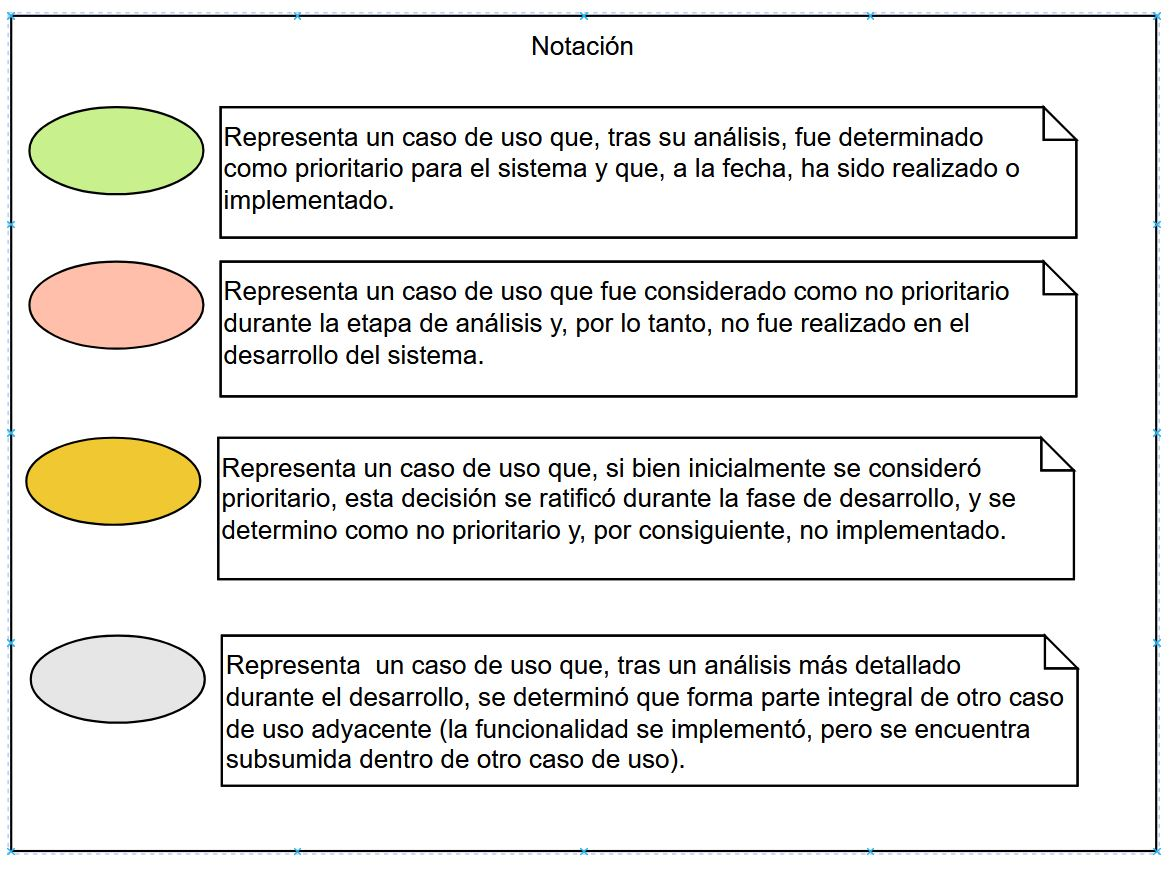
\includegraphics[width=.55\textwidth]{images/Notacion}}
		\caption{Análisis de viabilidad de los casos de uso.}
		\label{fig:Notacion}
	\end{center}
\end{figure}

A continuación, se detalla la notación empleada para la representación de los diagramas de casos de uso, la cual es fundamental para comprender la prioridad y el estado de implementación de cada funcionalidad del sistema. En la Figura \ref{fig:Notacion} se presenta la leyenda completa de esta notación, donde se utilizan cuatro colores distintos para clasificar los casos de uso según su análisis y desarrollo.


Los casos de uso representados en color verde fueron aquellos que, tras un análisis exhaustivo, se determinaron como prioritarios para la consecución de los objetivos principales del sistema y que, a la fecha, han sido completamente realizados o implementados. Esta categoría engloba las funcionalidades esenciales que sustentan la propuesta de valor de nuestro trabajo terminal.


Por otro lado, los casos de uso identificados con el color rojo fueron aquellos que, durante la etapa de análisis, se consideraron como no prioritarios para el alcance inicial del proyecto. En consecuencia, estas funcionalidades no fueron desarrolladas en la implementación del sistema.


Adicionalmente, se presenta una categoría de casos de uso en color amarillo. Estos casos fueron inicialmente considerados como prioritarios durante la fase de análisis; sin embargo, debido a diversos factores surgidos durante el desarrollo, se tomó la decisión de reconsiderar su prioridad y finalmente catalogarlos como no prioritarios, quedando fuera del alcance de la implementación actual.


Finalmente, los casos de uso representados en color gris son aquellos que, tras un análisis más detallado durante la etapa de desarrollo, se identificaron como componentes integrales de otros casos de uso adyacentes.


\subsection{Estructura de usuarios }

\begin{figure}[htbp!]
	\begin{center}
		\fbox{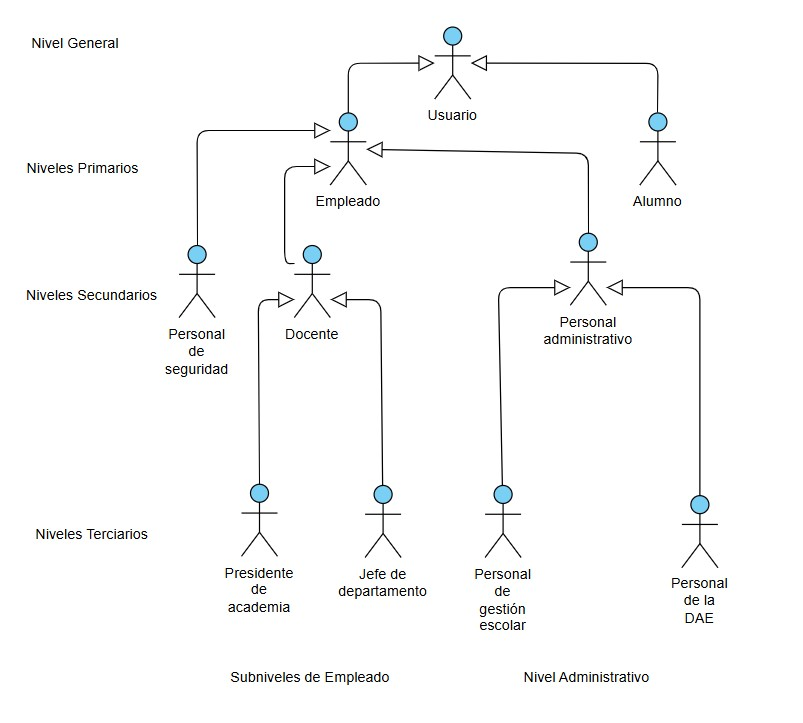
\includegraphics[width=.8\textwidth]{images/EstructuraU}}
		\caption{Estructura de los usuarios.}
		\label{fig:EstructuraU}
	\end{center}
\end{figure} 

En la Figura \ref{fig:EstructuraU} se ilustra la estructura jerárquica de los usuarios que interactúan con el sistema propuesto, detallando los diferentes tipos de roles y sus niveles de acceso. En el Nivel General, se encuentra el actor Usuario, que representa la abstracción más alta de cualquier entidad que interactúa con el sistema.

Del Usuario se derivan los Niveles Primarios: Empleado y Alumno. El Empleado engloba a todo el personal que labora en la institución, mientras que el Alumno representa a la población estudiantil.

Dentro del Nivel Primario de Empleado, encontramos los Subniveles de Empleado: Personal de seguridad y Docente. Estos roles poseen responsabilidades y permisos específicos dentro del sistema, diferenciándose de otros tipos de empleados.

También derivado del Empleado, se encuentra el Nivel Administrativo, representado por el actor Personal administrativo. Este nivel agrupa a roles con funciones de gestión y administración dentro del sistema, y se especializa en: Personal de gestión escolar, Presidente de academia, Jefe de departamento y Personal de la DAE (Dirección de administración Escolar). Cada uno de estos roles dentro del Nivel Administrativo tendrá permisos y accesos adaptados a sus responsabilidades específicas.

A continuación, se procederá a describir en detalle las responsabilidades y los procesos específicos de cada uno de los actores presentes en esta jerarquía.

%\newpage



%\newpage

%\newpage

\newpage

%---------------------------------------------------------
\subsection{Descripción de actores}

%---------------------------------------------------------
\begin{Usuario}{\hypertarget{tAlumno}{\subsubsection{Alumno}}}{
    Se refiere a las personas inscritas dentro de algún plan de estudios ofertado en la unidad académica.
}

\item[Responsabilidades:] \cdtEmpty
\begin{itemize}
    \item Asistir puntualmente a las clases, prácticas y evaluaciones.
    \item Respetar a docentes, compañeros y personal administrativo.
    \item Cumplir con los requisitos y actividades de las asignaturas inscritas, incluyendo tareas, proyectos y exámenes.
    \item Realizar oportunamente los trámites escolares como inscripciones, reinscripciones, solicitudes de documentos oficiales, etc.
    \item Portar credencial institucional en todo momento.
\end{itemize}
\textbf{Procesos clave:} \cdtEmpty
\begin{itemize}
    \item Inscribirse a asignaturas.
    \item Consultar calificaciones.
    \item Realizar pagos.
\end{itemize}
\end{Usuario}

\begin{Usuario}{\hypertarget{tPersonalSeguridad}{\subsubsection{Personal de seguridad}}}{
    Se refiere a las personas registradas como empleados y que permiten o no el acceso a la unidad académica.
}


\item[Responsabilidades:] \cdtEmpty
\begin{itemize}
    \item Supervisar el acceso y la salida de alumnos, personal docente y visitantes, asegurándose de que cumplan con los protocolos establecidos.
    \item Verificar la identificación de las personas que ingresan a las instalaciones.
    \item Responder de manera oportuna a incidentes o emergencias dentro de las instalaciones.
    \item Brindar apoyo al personal, docentes o alumnos en caso de accidentes o situaciones de riesgo.
\end{itemize}
\end{Usuario}

\begin{Usuario}{\hypertarget{tDocenteAplicador}{\subsubsection{Docente}}}{
    Se refiere a las personas registradas como empleados que dan clases a los alumnos y supervisan los ETS asignados.
}


\item[Responsabilidades:] \cdtEmpty
\begin{itemize}
    \item Impartir las clases de manera clara, puntual y completa, cumpliendo con los objetivos de aprendizaje.
    \item Diseñar y aplicar instrumentos de evaluación justos, objetivos y alineados con los contenidos del curso.
    \item Orientar a los alumnos en el desarrollo de competencias y habilidades.
    \item Resolver dudas o problemáticas académicas dentro y fuera del aula, cuando sea necesario.
    \item Registrar la asistencia de los alumnos y reportar incidencias graves.
    \item Cumplir con la entrega de calificaciones y reportes en tiempo y forma.
\end{itemize}
\end{Usuario}

\begin{Usuario}{\hypertarget{tPersonalGestion}{\subsubsection{Personal de gestión escolar}}}{
    Se refiere a las personas registradas como empleados y personal administrativo que realiza los procesos administrativos dentro de la ESCOM.
}
\item[Responsabilidades:] \cdtEmpty
\begin{itemize}
    \item Gestionar el proceso de inscripción y reinscripción de los alumnos, verificando que cumplan con los requisitos establecidos.
    \item Mantener y actualizar el historial académico de los alumnos en los sistemas institucionales.
    \item Revisar y validar actas de nacimiento, certificados y otros documentos oficiales requeridos para el registro de los alumnos.
    \item Atender solicitudes y problemáticas relacionadas con registros, certificados, bajas temporales y procesos extraordinarios.
    \item Brindar orientación a alumnos y docentes sobre trámites escolares, fechas importantes y normatividad académica.
\end{itemize}
\end{Usuario}

\begin{Usuario}{\hypertarget{tPersonalDAE}{\subsubsection{Personal de la DAE}}}{
    Se refiere a las personas registradas como empleados y personal administrativo que realiza los procesos administrativos dentro de la DAE.
}

\item[Responsabilidades:] \cdtEmpty
\begin{itemize}
    \item Fomentar y coordinar actividades extracurriculares que complementen la formación académica, como talleres, conferencias, eventos culturales y deportivos.
    \item Supervisar programas de apoyo académico, como tutorías, orientación educativa y psicológica.
    \item Difundir información sobre programas de movilidad académica, intercambios, convenios nacionales e internacionales y programas de servicio social.
    \item Gestionar y emitir las credenciales oficiales del IPN para los alumnos.
    \item Verificar que los documentos requeridos para la emisión de la credencial estén completos y sean válidos.
    \item Coordinar el proceso de inscripción de los alumnos.
    \item Actualizar y mantener los registros académicos y administrativos de los alumnos. 

\end{itemize}
\end{Usuario}


\begin{Usuario}{\hypertarget{tPresidente}{\subsubsection{Presidente de academia}}}{
Se refiere a las personas registradas como empleados y personal administrativo que lidera la academia de una unidad académica o área de conocimiento dentro de la ESCOM.
}
\item[Responsabilidades:] \cdtEmpty
\begin{itemize}
    \item Convocar y presidir las reuniones de academia, donde se toman decisiones sobre planes y programas de estudio.
    \item Coordinar la creación o actualización de planes y programas de estudio conforme a las necesidades del mercado laboral y las directrices institucionales.
    \item Verificar que los contenidos impartidos por los docentes sean consistentes con los objetivos de los programas.
    \item Detectar necesidades de capacitación entre los docentes y promover cursos o talleres. 
\end{itemize}
\end{Usuario}

\begin{Usuario}{\hypertarget{tJefe}{\subsubsection{Jefe de departamento}}}{
Se refiere a las personas registradas como empleados y personal administrativo que supervisa las actividades de una o más unidades académicas dentro de ESCOM.
}
\item[Responsabilidades:] \cdtEmpty
\begin{itemize}
\item Administrar los recursos humanos y materiales asignados al departamento.
\item Supervisar la implementación de los programas de estudio y el cumplimiento de los objetivos educativos.
\item Promover y coordinar proyectos de investigación, desarrollo tecnológico o vinculación relacionados con el departamento.
\item Atender quejas, sugerencias o problemas que surjan en el departamento, ya sea entre docentes o alumnos.
\end{itemize}
\end{Usuario}



\newpage

\subsection{Diagramas de casos de uso}

A continuación se muestran los diagramas de casos de uso:


\begin{figure}[htbp!]
	\begin{center}
		\fbox{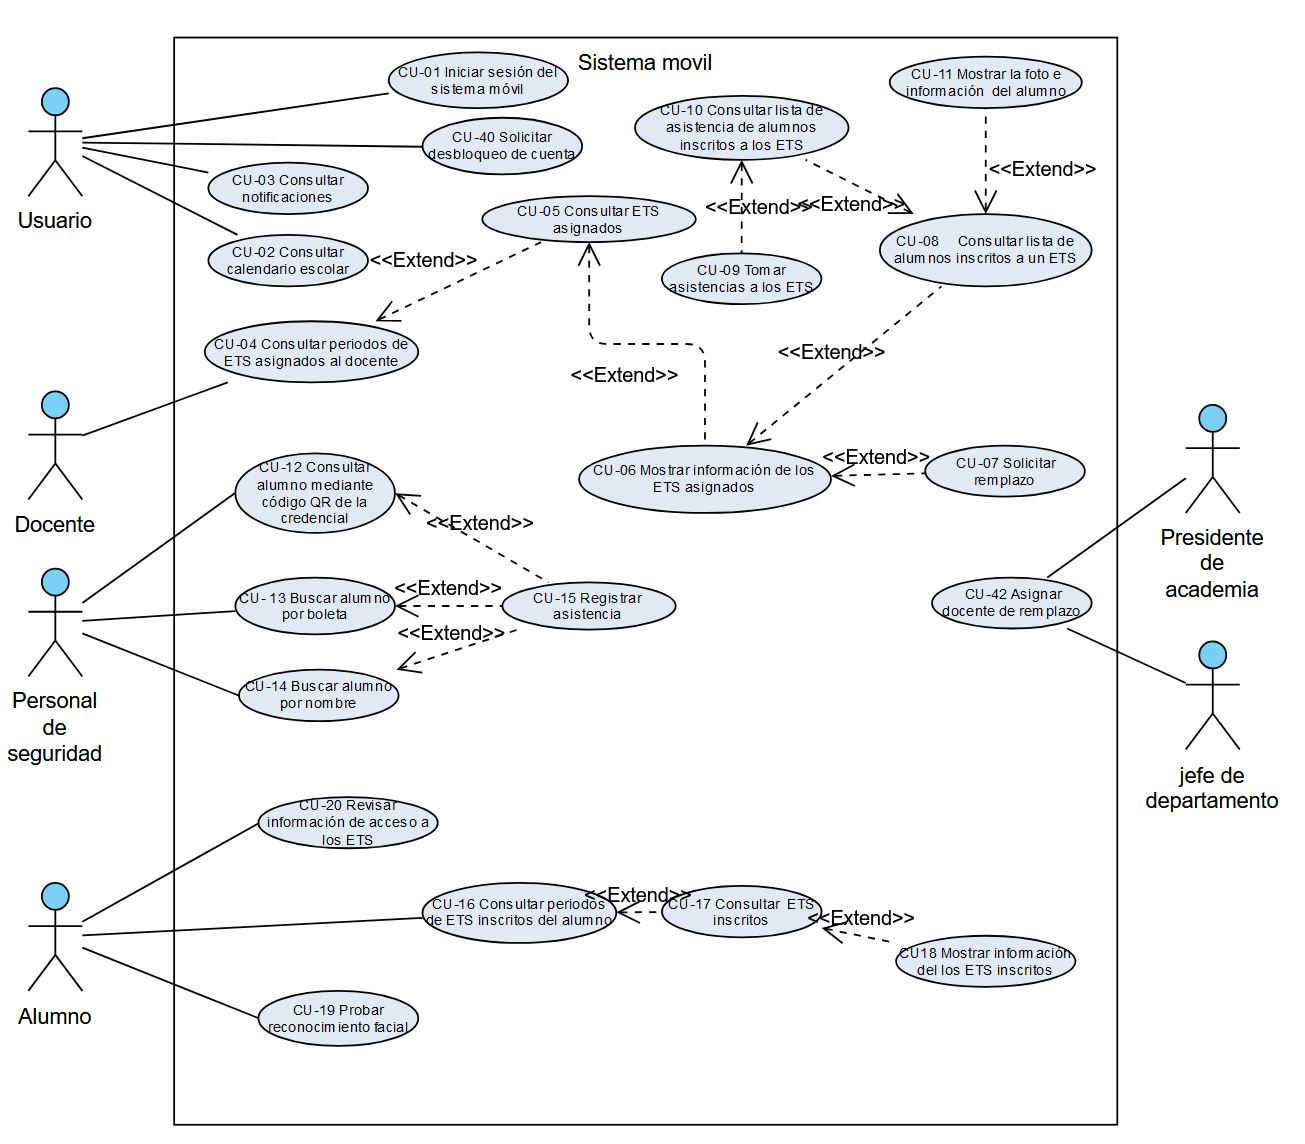
\includegraphics[width=.9\textwidth]{images/casosDeUso1}}
		\caption{Diagrama de casos de uso del sistema movil.}
		\label{fig:casosDeUso1}
	\end{center}
\end{figure}

En la Figura \ref{fig:casosDeUso1} se presenta el diagrama de casos de uso del sistema móvil, el cual constituye el núcleo central del presente trabajo terminal. Este diagrama detalla la estructura funcional del sistema, así como las interacciones específicas de los siguientes actores: Alumno, Docente, Personal de seguridad, Presidente de academia y Jefe de departamento. La notación de colores empleada en este diagrama (detallada en la Figura \ref{fig:Notacion}) permite identificar la prioridad y el estado de cada caso de uso.
Como se observa, la mayoría de los casos de uso se presentan en color verde, indicando su prioridad y realización dentro del proyecto. Sin embargo, existen algunas excepciones que merecen una explicación detallada:


El caso de uso CU-03 (Consultar notificaciones) se presenta en color amarillo. Esta decisión se tomó durante la fase de desarrollo, al identificar que su implementación completa a lo largo del ciclo de vida del proyecto presentaba una complejidad significativa. Adicionalmente, se consideró que el valor añadido de esta funcionalidad a la experiencia general del usuario no justificaba el esfuerzo requerido para su desarrollo en el alcance actual del proyecto.


Los casos de uso CU-04 (Consultar periodos de ETS asignados al docente) y CU-16 (Consultar periodos de ETS inscritos del alumno) también se identifican con el color amarillo. La determinación de no priorizar la separación de la consulta de ETS por periodos se basó en la evaluación de su impacto en la funcionalidad principal del sistema. Se concluyó que esta distinción no aportaba un valor significativo a la experiencia del usuario y que la revisión especifica de ETS por periodo carecía de relevancia práctica dentro del contexto del sistema propuesto.


El caso de uso CU-40 (Solicitar desbloqueo de cuenta) se presenta en color amarillo debido a una limitación técnica inherente a la arquitectura supuesta del sistema. Al considerar que el sistema móvil opera en conexión directa con los registros de la plataforma original del SAES (Sistema de Administración Escolar), la funcionalidad de bloquear o cambiar contraseñas desde la aplicación móvil se consideró inviable y fuera del alcance, ya que estas operaciones se gestionarían directamente a través de la plataforma original SAES.


Finalmente, el caso de uso CU-10 (Consultar lista de asistencia de alumnos inscritos al ETS) se presenta en color gris y se encuentra enlazado mediante una relación de inclusión al caso de uso CU-08 (Consultar lista de alumnos inscritos a un ETS). Esta decisión de diseño se tomó con el objetivo de optimizar la experiencia del usuario, integrando la visualización de ambas listas, es decir se muestra la lista de los alumnos inscritos al ETS y el estado de asistencia (si se presentó o no al ETS).


Los demás casos de uso presentados en color verde representan las funcionalidades prioritarias y ya implementadas del sistema móvil, las cuales serán explicadas en la sección de detalles de los casos de uso.


\newpage

%\newpage
\begin{figure}[htbp!]
	\begin{center}
		\fbox{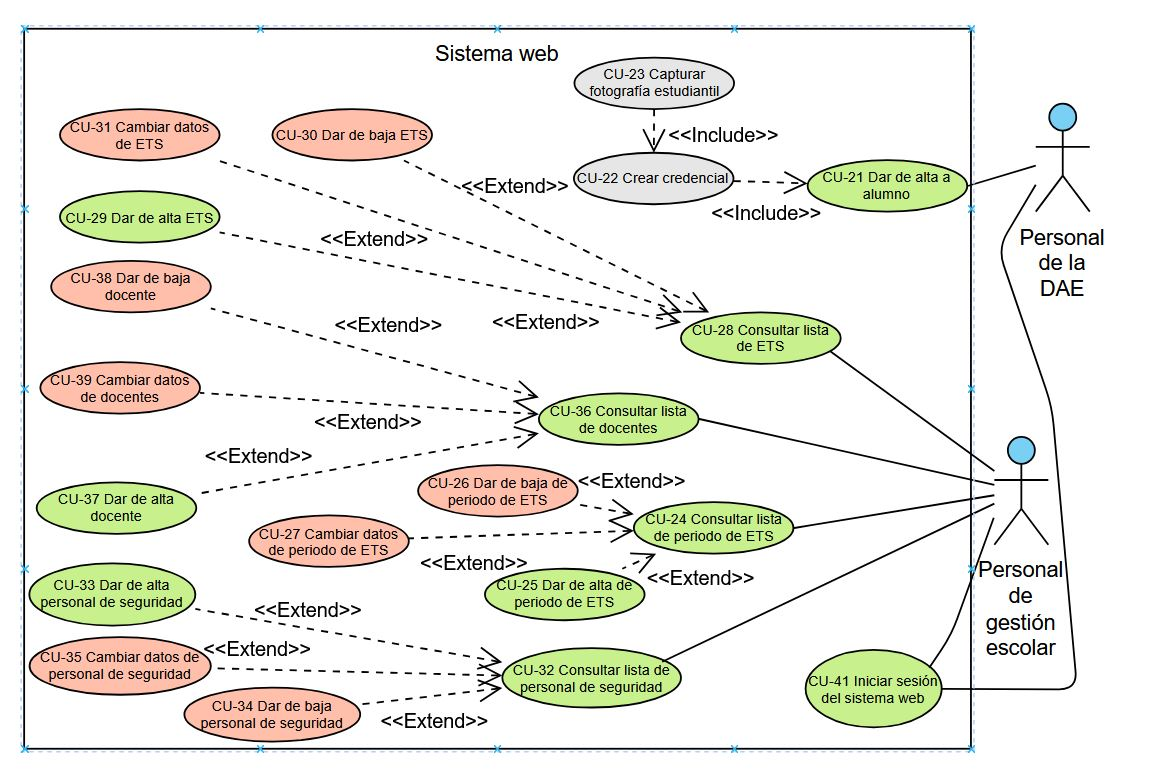
\includegraphics[width=.9\textwidth]{images/casosDeUso2}}
		\caption{Diagrama de casos de uso del sistema web.}
		\label{fig:casosDeUso2}
	\end{center}
\end{figure}


En la Figura \ref{fig:casosDeUso2} se presenta el diagrama de casos de uso correspondiente al sistema web. Este diagrama ilustra las funcionalidades a las que tienen acceso principalmente el Personal de la DAE y el Personal de gestión escolar, complementando las funcionalidades ofrecidas por el sistema móvil. Al igual que en el diagrama del sistema móvil, se utiliza la notación de colores previamente definida para indicar la prioridad y el estado de implementación de cada caso de uso.

La mayoría de los casos de uso en este diagrama se presentan en color verde, lo que indica que fueron considerados prioritarios y han sido realizados. Estos casos de uso abarcan la gestión de información y procesos administrativos relevantes para los roles del Personal de la DAE y el Personal de gestión escolar.

Sin embargo, es importante destacar la relación existente entre los casos de uso CU-21 (Dar de alta a alumno), CU-22 (Crear credencial) y CU-23 (Capturar fotografía estudiantil). Inicialmente concebidos como funcionalidades separadas, durante la fase de desarrollo se tomó la decisión de unificarlos dentro del caso de uso CU-21. Esta integración se realizó con el objetivo de optimizar la experiencia del usuario, permitiendo que el Personal de la DAE realice el alta del alumno, la captura de su fotografía y la creación de la credencial en una única pantalla o flujo de proceso. 

\subsection{Detalle de los casos de uso}

%---------------------------------------------------------
% CASOS DE USO

% !TeX root = ../ejemplo.tex

%--------------------------------------
\label{CU-01}
\begin{UseCase}{CU-01}{Iniciar sesión del sistema móvil}{
		
		Permitir que solo los usuarios registrados en el sistema móvil puedan acceder a este, además de separar completamente las funciones de los usuarios del sistema móvil.
	}
	\UCitem{Versión}{\color{Gray}1}
	\UCitem{Autor}{\color{Gray}Huertas Ramírez Daniel Martín.}
	\UCitem{Supervisa}{\color{Gray}De la Cruz de la Cruz Alejandra.}
	\UCitem{Actor}{ \hyperlink{tDocente}{Docente}, \hyperlink{tPersonalSeguridad}{Personal de seguridad}, \hyperlink{tAlumno}{Alumno}, \hyperlink{tPresidente}{Presidente de academia} y \hyperlink{tJefe}{Jefe de departamento} }
	\UCitem{Propósito}{Que el usuario del sistema móvil pueda acceder al sistema móvil y sus funciones específicas.}
	\UCitem{Entradas}{ En caso del \hyperlink{tPersonalSeguridad}{Personal de seguridad}, ingresará con su CURP y Contraseña. En caso del alumno con su Boleta y Contraseña. En caso del \hyperlink{tDocente}{Docente}, \hyperlink{tPresidente}{Presidente de academia} y \hyperlink{tJefe}{Jefe de departamento} se usará su RFC y su Contraseña}
	\UCitem{Origen}{Pantalla táctil}
	\UCitem{Salidas}{Saludo del sistema y mención de su nombre.}
	\UCitem{Destino}{Pantalla \IUref{IUE01}{Pantalla de saludo del docente} si es un docente, a la \IUref{IUE02}{Pantalla de saludo del personal de seguridad} si es un personal de seguridad, a la \IUref{IUE03}{Pantalla de saludo del alumno} si es un alumno y a la \IUref{IUE06}{Pantalla de saludo del presidente de academia/jefe de departamento} si es un presidente de academia o jefe de departamento.}
	\UCitem{Precondiciones}{El usuario debe estar registrado en el sistema móvil.}
	\UCitem{Postcondiciones}{El usuario accede al sistema móvil y podrá realizar las acciones pertinentes a su rol.}
	\UCitem{Errores}{
		E1: Cuando falte algún dato requerido entonces el sistema muestra el mensaje \textbf{``Por favor, completa todos los campos.''}
		
		E2: Cuando los datos no concuerdan con ninguna cuenta de usuario, se muestra el mensaje \textbf{ ``Datos incorrectos.''}
		
		E3: Cuando se pierde la conexión durante el proceso, los procesos se cancelan y se muestra el mensaje \textbf{ ``Conexión perdida.''}
	}
	\UCitem{Tipo}{Caso de uso primario}
	\UCitem{Observaciones}{}
\end{UseCase}
%--------------------------------------

\begin{UCtrayectoria}
	\UCpaso[\UCactor] El usuario inicia la aplicación y accede a la pantalla \IUref{IU01}{Iniciar sesión del sistema móvil}.
	\UCpaso[\UCactor] Si el usuario es un alumno, introduce su número de boleta y su contraseña. Si el usuario es Personal de seguridad, introduce su CURP y contraseña. Si el usuario es Docente, Presidente de academia o Jefe de departamento, introduce su RFC y contraseña en el sistema a través de la \IUref{IU01}{Iniciar sesión del sistema móvil}\label{CU01.introduceDatos}.
	\UCpaso[\UCactor] El usuario confirma la operación presionando el botón \IUbutton{Entrar}.
	\UCpaso El sistema verifica que todos los datos requeridos hayan sido capturados.
	\UCpaso El sistema verifica que el usuario esté registrado en el sistema.
	\UCpaso El sistema verifica que la contraseña proporcionada corresponde al usuario identificado.
	\UCpaso El sistema determina el rol del usuario que ha iniciado sesión.
	\UCpaso La sesión se inicia con éxito.
	\UCpaso El usuario es redirigido a la {Pantalla \IUref{IUE01}{Pantalla de saludo del docente} si es un docente, a la \IUref{IUE02}{Pantalla de saludo del personal de seguridad} si es un personal de seguridad, a la \IUref{IUE03}{Pantalla de saludo del alumno} si es un alumno y a la \IUref{IUE06}{Pantalla de saludo del presidente de academia/jefe de departamento} si es un presidente de academia o jefe de departamento}.
\end{UCtrayectoria}





\newpage

% !TeX root = ../ejemplo.tex

%--------------------------------------
\begin{UseCase}{CU-02}{Consultar calendario escolar}{
    Permitir que los usuarios vean el calendario escolar y puedan solicitar al sistema que les mencioné cuantos días faltan para que inicie el próximo periodo de ETS.
}
    \UCitem{Versión}{\color{Gray}1}
    \UCitem{Autor}{\color{Gray}Huertas Ramírez Daniel Martín}
    \UCitem{Supervisa}{\color{Gray}De la Cruz de la Cruz Alejandra.}
    \UCitem{Actor}{\hyperlink{Usuario}{Usuario}}
    \UCitem{Propósito}{Que el usuario consulte cuantos días faltan para el próximo periodo de ETS.}
    \UCitem{Entradas}{Ninguna}
    \UCitem{Origen}{Pantalla táctil}
    \UCitem{Salidas}{Menciona cuantos días faltan para el periodo de ETS o si menciona que ya es periodo de ETS.}
    \UCitem{Destino}{Ninguno}
    \UCitem{Precondiciones}{El usuario debe de haber iniciado sesión.}
    \UCitem{Postcondiciones}{El usuario recibe información sobre la fecha del periodo de ETS actual.}
    \UCitem{Errores}{
        E1: Cuando es periodo de ETS el sistema muestra el mensaje {\bf MSG-6}{``Actualmente es periodo de ETS.''}

        E2: Cuando no se ha establecido un periodo de ETS actual, el sistema muestra el mensaje {\bf MSG-7}{``Actualmente el periodo de ETS no ha sido establecido.''}
    
    }
    \UCitem{Tipo}{Caso de uso primario}
    \UCitem{Observaciones}{Ninguna}
\end{UseCase}
%-------------------------------------- 

\begin{UCtrayectoria}
    \UCpaso[\UCactor] El usuario accede a la pantalla \IUref{IU02}{Pantalla Consultar calendario escolar}\label{CU02.introduceDatos} para la app móvil mediante el botón con forma de calendario en cualquier pantalla excepto el inicio de sesión.
    \UCpaso[\UCactor] El usuario decide consultar cuantos días faltan para que el periodo de ETS inicie oprimiendo el botón\IUbutton{Calcular cuantos días faltan para el periodo de ETS}.
    \UCpaso El sistema calcula cuantos días faltan tomando el día actual y el día de inicio del periodo de ETS.
    \UCpaso El sistema regresa cuantos días faltan para que el periodo de ETS inicie.
    \UCpaso [\UCactor] El usuario verifica cuantos días faltan para que inicie el periodo de ETS.
\end{UCtrayectoria}








\newpage

%% !TeX root = ../ejemplo.tex

%--------------------------------------
\begin{UseCase}{CU-03}{Consultar notificaciones}{
    Permitir a los usuarios revisar sus notificaciones con más detenimiento y establecerlas como leídas.
}
    \UCitem{Versión}{\color{Gray}1}
    \UCitem{Autor}{\color{Gray}Huertas Ramírez Daniel Martín}
    \UCitem{Supervisa}{\color{Gray}De la Cruz de la Cruz Alejandra.}
    \UCitem{Actor}{\hyperlink{Usuario}{Usuario}}
    \UCitem{Propósito}{Que el usuario revise sus notificaciones con detenimiento y las establezca como leídas.}
    \UCitem{Entradas}{Ninguna}
    \UCitem{Origen}{Pantalla táctil}
    \UCitem{Salidas}{Menciona que la notificación seleccionada ha sido establecida como leída.}
    \UCitem{Destino}{Ninguno}
    \UCitem{Precondiciones}{El usuario debe de haber iniciado sesión.}
    \UCitem{Postcondiciones}{El usuario revisó sus notificaciones.}
    \UCitem{Errores}{
        E1: Cuando el usuario no tiene notificaciones el sistema muestra el mensaje {\bf MSG-8}{``Actualmente no hay notificaciones.''}    
    }
    \UCitem{Tipo}{Caso de uso primario}
    \UCitem{Observaciones}{}

\end{UseCase}
%-------------------------------------- 

\begin{UCtrayectoria}
    \UCpaso[\UCactor] El usuario accede a la pantalla \IUref{IU03}{Pantalla Consultar notificaciones}\label{CU03.introduceDatos} para la app móvil  mediante el botón con forma de campana en cualquier pantalla excepto los inicios de sesión.
    \UCpaso[\UCactor] El usuario decide consultar sus notificaciones más actuales \Trayref{A}.
    \UCpaso[\UCactor] El usuario marco como leídas las notificaciones que acaba de leer mediante el botón con forma de palomita especifico de cada notificación.
    \UCpaso El sistema marca como leídas las notificaciones.

\end{UCtrayectoria}

\begin{UCtrayectoriaA}{A}{El usuario quiere consultar las notificaciones de una fecha específica}
	\UCpaso[\UCactor] El usuario usa el buscador de la parte superior para buscar notificaciones según su fecha.
	\UCpaso[\UCactor] El usuario marco como leídas las notificaciones que acaba de leer mediante el botón con forma de palomita especifico de cada notificación.
	\UCpaso El sistema marca como leídas las notificaciones.

\end{UCtrayectoriaA}



%\newpage

%% \IUref{IUAdmPS}{Administrar Planta de Selección}
% \IUref{IUModPS}{Modificar Planta de Selección}
% \IUref{IUEliPS}{Eliminar Planta de Selección}

%-------------------------------------- COMIENZA descripción del caso de uso.

%\begin{UseCase}[archivo de imágen]{UCX}{Nombre del Caso de uso}{
%--------------------------------------
% !TeX root = ../ejemplo.tex
\begin{UseCase}{CU-04}{Consultar periodos de ETS asignados al docente}{
	Este caso de uso permite al docente consultar los periodos de ETS que tiene asignados. 
}
\UCitem{Versión}{\color{Gray}1.0} 
\UCitem{Autor}{\color{Gray}De la cruz De la cruz Alejandra}
\UCitem{Supervisa}{\color{Gray}Huertas Ramírez Daniel Martín }
\UCitem{Actor}{\hyperlink{Docente}{Docente}}
\UCitem{Propósito}{Permitir al docente consultar los periodos de ETS que le han sido asignados.}
\UCitem{Entradas}{Ninguna}
\UCitem{Origen}{Pantalla táctil}
\UCitem{Salidas}{Lista de periodos de ETS asignados.}
\UCitem{Destino}{\IUref{IU04}{Pantalla Periodo de ETS}}
\UCitem{Precondiciones}{El docente debe estar autenticado en el sistema.}
\UCitem{Postcondiciones}{El docente ha consultado los periodos de ETS asignados.}
\UCitem{Errores}{
		E1: El sistema no puede recuperar la información de los periodos y muestra el mensaje {\bf MSG-9}{``Error al consultar la base de datos. Intente nuevamente más tarde''.}
		
		E2: No hay periodos de ETS asignados al docente y se muestra el mensaje {\bf MSG-10}{``No tienes periodos de ETS asignados.''}
}
\UCitem{Tipo}{Se entiende del CU-01 Iniciar sesión del sistema móvil}
\UCitem{Observaciones}{Ninguna}
\end{UseCase}
%--------------------------------------
\begin{UCtrayectoria}
\UCpaso[\UCactor] El docente accede a la \IUref{IUE01}{Pantalla saludo del docente} después de haber iniciado sesión.
\UCpaso[\UCactor] El docente presiona el botón \IUbutton{Consultar periodos de ETS}.
\UCpaso El sistema verifica que el docente cuente con periodos de ETS. \Trayref{A}.
\UCpaso El sistema busca en la base de datos los periodos de ETS asignados al docente.
\UCpaso El sistema despliega la lista de periodos de ETS asignados al docente en la \IUref{IU04}{Pantalla Periodo de ETS}.
\end{UCtrayectoria}
%--------------------------------------        
\begin{UCtrayectoriaA}{A}{No hay periodos asignados al docente}
\UCpaso El sistema verifica y no encuentra registros de periodos de ETS asignados al docente.
\UCpaso El sistema muestra un mensaje: {\bf MSG-10}{`` No tienes periodos de ETS asignados.''}
\UCpaso[\UCactor] El docente presiona el botón \IUbutton{Regresar} para volver a la pantalla anterior.
\UCpaso Fin de la trayectoria alternativa.
\end{UCtrayectoriaA}
%--------------------------------------        
\begin{UCtrayectoriaA}{B}{Error en la conexión con la base de datos}
\UCpaso El sistema muestra un mensaje de error: {\bf MSG-9}{``Error al consultar la base de datos. Intente nuevamente más tarde.''}
\UCpaso[\UCactor] El docente resiona el botón \IUbutton{Aceptar} para cerrar el mensaje.
\UCpaso[\UCactor] El docente puede intentar la consulta nuevamente o presionar el botón \IUbutton{Regresar} para volver a la pantalla anterior.
\UCpaso Fin de la trayectoria alternativa.
\end{UCtrayectoriaA}
%-------------------------------------- TERMINA descripción del caso de uso.

%\newpage

% \IUref{IUAdmPS}{Administrar Planta de Selección}
% \IUref{IUModPS}{Modificar Planta de Selección}
% \IUref{IUEliPS}{Eliminar Planta de Selección}

%-------------------------------------- COMIENZA descripción del caso de uso.

%\begin{UseCase}[archivo de imágen]{UCX}{Nombre del Caso de uso}{
%--------------------------------------
\label{CU-05}
\begin{UseCase}{CU-05}{Consultar ETS asignados}{
		Este caso de uso permite al docente consultar los ETS que tiene asignados.
	}
	\UCitem{Versión}{\color{Gray}2.0}
	\UCitem{Autor}{\color{Gray}De la cruz De la cruz Alejandra}
	\UCitem{Supervisa}{\color{Gray}Huertas Ramírez Daniel Martín}
	\UCitem{Actor}{\hyperlink{tDocente}{Docente}}
	\UCitem{Propósito}{Permitir al docente consultar los ETS que le han sido asignados.}
	\UCitem{Entradas}{Solicitud de consulta.}
	\UCitem{Origen}{Pantalla táctil}
	\UCitem{Salidas}{Lista de ETS asignados (Unidad de Aprendizaje, Periodo, Fecha, Turno) o indicación de que no hay ETS asignados.}
	\UCitem{Destino}{\IUref{IU06}{Pantalla de Consultar ETS}}
	\UCitem{Precondiciones}{El docente debe haber iniciado sesión en el sistema (\textbf{\hyperref[CU-01]{CU-01 Iniciar sesión del sistema móvil}}).}
	\UCitem{Postcondiciones}{El docente ha consultado los ETS asignados.}
	\UCitem{Errores}{
		E1: El sistema no puede recuperar la información de los ETS asignados y se muestra el mensaje \textbf{``Error al consultar la base de datos. Intente nuevamente más tarde.''}.
		
		E2: Cuando se pierde la conexión durante el proceso, los procesos se cancelan y se muestra el mensaje \textbf{ ``Conexión perdida.''}
	}
	\UCitem{Tipo}{Caso de uso primario}
	\UCitem{Observaciones}{Ninguna}
\end{UseCase}
%--------------------------------------
\begin{UCtrayectoria}
	\UCpaso[\UCactor] El docente accede a la \IUref{IU05}{Pantalla de Consultar ETS} desde el menú principal.
	\UCpaso El sistema recupera la lista de todos los ETS asignados al docente.
	\UCpaso El sistema muestra la lista de ETS, incluyendo para cada uno: Unidad de Aprendizaje, Periodo, Fecha y Turno.
	\UCpaso[\UCactor] El docente visualiza la lista de ETS asignados.
	\UCpaso[\UCactor] El docente selecciona un ETS de la lista.
	\UCpaso El sistema redirige al docente a la pantalla \IUref{IU06}{Pantalla Información de ETS}.
	\UCpaso[\UCactor] Opcionalmente, el docente puede presionar el botón \IUbutton{Todos} para ver todos los ETS asignados.
	\UCpaso[\UCactor] Opcionalmente, el docente puede presionar el botón \IUbutton{Mis ETS} para ver los ETS que tiene pendientes por aplicar o supervisar.
\end{UCtrayectoria}

%--------------------------------------
\begin{UCtrayectoriaA}{A}{No hay ETS asignados}
	\UCpaso El sistema verifica que no hay ETS asignados al docente.
	\UCpaso El sistema muestra el mensaje \textbf{``No hay ETS creados.''} indicando que no hay ETS asignados.
	\UCpaso[\UCactor] El docente visualiza el mensaje.
	\UCpaso[\UCactor] El docente presiona el botón \IUbutton{Regresar} para volver a la pantalla anterior.
	\UCpaso Fin de la trayectoria alternativa.
\end{UCtrayectoriaA}

%--------------------------------------
\begin{UCtrayectoriaA}{B}{Error en la conexión con la base de datos}
	\UCpaso El sistema intenta recuperar la lista de ETS asignados.
	\UCpaso Ocurre un error en la conexión con la base de datos.
	\UCpaso El sistema muestra el mensaje de error: \textbf{``Error al consultar la base de datos. Intente nuevamente más tarde.''}.
	\UCpaso[\UCactor] El docente presiona el botón \IUbutton{Aceptar} para cerrar el mensaje.
	\UCpaso[\UCactor] El docente puede intentar la consulta nuevamente o presionar el botón \IUbutton{Regresar} para volver a la pantalla anterior.
	\UCpaso Fin de la trayectoria alternativa.
\end{UCtrayectoriaA}

%-------------------------------------- TERMINA descripción del caso de uso.
\newpage

% \IUref{IUAdmPS}{Administrar Planta de Selección}
% \IUref{IUModPS}{Modificar Planta de Selección}
% \IUref{IUEliPS}{Eliminar Planta de Selección}

%-------------------------------------- COMIENZA descripción del caso de uso.

%\begin{UseCase}[archivo de imágen]{UCX}{Nombre del Caso de uso}{
%--------------------------------------
% !TeX root = ../ejemplo.tex
\begin{UseCase}{CU-06}{Mostrar información de los ETS asignados}{
	Este caso de uso permite al docente visualizar la información detallada de los ETS que tiene asignados.
}
\UCitem{Versión}{\color{Gray}1.0}
\UCitem{Autor}{\color{Gray}De la cruz De la cruz Alejandra}
\UCitem{Supervisa}{\color{Gray}Huertas Ramírez Daniel Martín}
\UCitem{Actor}{\hyperlink{PersonalAcademico}{Docente}}
\UCitem{Propósito}{Permite al docente visualizar la información detallada de cada ETS que tiene asignado.}
\UCitem{Entradas}{Ninguna}
\UCitem{Origen}{Pantalla táctil}
\UCitem{Salidas}{Detalle de ETS asignado.}
\UCitem{Destino}{\IUref{IU06}{Pantalla Información de ETS}}
\UCitem{Precondiciones}{El docente debe estar autenticado y tener ETS asignados en el sistema.}
\UCitem{Postcondiciones}{El docente ha visualizado la información detallada de sus ETS asignados.}
\UCitem{Errores}{
		E1: El sistema no puede recuperar la información detallada de los ETS y muestra el mensaje {\bf MSG-12}{``Información no disponible para el ETS seleccionado''}.
		E2: Error en la conexión con la base de datos y muestra el mensaje y muestra el mensaje {\bf MSG-9}{``Error al consultar la base de datos. Intente nuevamente más tarde.''}.
}
\UCitem{Tipo}{Se entiende del CU-05 Mostrar información de los ETS asignados}
\UCitem{Observaciones}{Ninguna}
\end{UseCase}
%--------------------------------------
\begin{UCtrayectoria}
\UCpaso[\UCactor] El docente selecciona el ETS que desea visualizar desde la \IUref{IU05}{Pantalla  Consultar ETS}.
\UCpaso[\UCsist] El sistema verifica si existen detalles disponibles para el ETS seleccionado. \Trayref{A}
\UCpaso El sistema despliega la información detallada de cada ETS asignado en la \IUref{IU06}{Pantalla Información de ETS}
\end{UCtrayectoria}
%--------------------------------------        
\begin{UCtrayectoriaA}{A}{No hay detalles disponibles para el ETS seleccionado}
\UCpaso El sistema muestra un mensaje: {\bf MSG-12}{``Información no disponible para el ETS seleccinado''}
\UCpaso[\UCactor] El docente presiona el botón \IUbutton{Regresar} para volver a la lista de ETS.
\UCpaso Fin de la trayectoria alternativa.
\end{UCtrayectoriaA}

%--------------------------------------        
\begin{UCtrayectoriaA}{B}{Error en la conexión con la base de datos}
\UCpaso El sistema muestra un mensaje de error: {\bf MSG-9}{``Error al consultar la base de datos. Intente nuevamente más tarde.''}
\UCpaso[\UCactor] El docente presiona el botón \IUbutton{Aceptar} para cerrar el mensaje.
\UCpaso[\UCactor] El docente puede intentar la consulta nuevamente o presionar el botón \IUbutton{Regresar} para volver a la pantalla anterior.
\UCpaso Fin de la trayectoria alternativa.
\end{UCtrayectoriaA}

%-------------------------------------- TERMINA descripción del caso de uso.


\newpage

% \IUref{IUAdmPS}{Administrar Planta de Selección}
% \IUref{IUModPS}{Modificar Planta de Selección}
% \IUref{IUEliPS}{Eliminar Planta de Selección}

%-------------------------------------- COMIENZA descripción del caso de uso.

%\begin{UseCase}[archivo de imágen]{UCX}{Nombre del Caso de uso}{
%--------------------------------------
\begin{UseCase}{CU-07}{Solicitar remplazo }{
	Este caso de uso permite a un docente solicitar un reemplazo para que aplique el ETS cuando no pueda asistir.
}
\UCitem{Versión}{\color{Gray}1.0}
\UCitem{Autor}{\color{Gray}De la cruz De la cruz Alejandra}
\UCitem{Supervisa}{\color{Gray}Huertas Ramírez Daniel}
\UCitem{Actor}{\hyperlink{PersonalAcademico}{Docente}}
\UCitem{Propósito}{Permitir al docente responsable de un ETS solicitar apoyo de otro profesor para llevar a cabo la aplicación, notificando al jefe de departamento o al presidente de academia.}
\UCitem{Entradas}{Identificador del ETS y razón por la que se pide el remplazo.}
\UCitem{Origen}{Pantalla táctil}
\UCitem{Salidas}{
	Se muestra el mensaje \textbf{``Solicitud exitosa. La solicitud de reemplazo ha sido registrada correctamente'', indicando que la solicitud fue enviada con éxito.}
	
	Se muestra el mensaje \textbf{: ``Ya existe una solicitud pendiente para este ETS'', indicando que ya se ha realizado una solicitud previa para el ETS.}
	}
\UCitem{Destino}{\IUref{IU06}{Pantalla Información de ETS}}
\UCitem{Precondiciones}{El docente debe estar autenticado en el sistema y tener un ETS asignado.}
\UCitem{Postcondiciones}{La solicitud ha sido enviada al jefe de departamento y/o al presidente de academia.}
\UCitem{Errores}{
	E1: Cuando se pierde la conexión durante el proceso, los procesos se cancelan y se muestra el mensaje {\bf  ``Error al enviar la solicitud''}
}
\UCitem{Tipo}{Se entiende del CU-06 Mostrar información de los ETS asignados}
\UCitem{Observaciones}{Ninguna}
\end{UseCase}
%--------------------------------------
\begin{UCtrayectoria}
\UCpaso[\UCactor] El docente accede a la \IUref{IU06}{Pantalla Información de ETS}.
\UCpaso[\UCactor] El docente selecciona la opción \IUbutton{Solicitar reemplazo} para el ETS asignado.
\UCpaso El sistema redirige al docente a la pantalla \IUref{IU07}{ Solicitar remplazo }.
\UCpaso El sistema muestra el ETS selecciona.
\UCpaso[\UCactor] El docente ingresa la razón para solicitar el remplazo.
\UCpaso[\UCactor] El docente oprime el botón \IUbutton{Enviar solicitud} [Trayectoria A] [Trayectoria B] .
\UCpaso El sistema envía la solicitud de remplazo al jefe de departamento y/o al presidente de academia.
\end{UCtrayectoria}
%--------------------------------------        
\begin{UCtrayectoriaA}{A}{Ya existe una solicitud pendiente para el ETS}
	\UCpaso El sistema valida que exista una solicitud previa no resuelta.
	\UCpaso El sistema muestra el mensaje: {\bf``Ya existe una solicitud pendiente para este ETS''}.
	\UCpaso[\UCactor] El docente presiona \IUbutton{Aceptar} para regresar a \IUref{IU06}{Pantalla Información de ETS}.
\end{UCtrayectoriaA}
%-------------------------------------- TERMINA descripción del caso de uso.
\begin{UCtrayectoriaA}{B}{Error al enviar la solicitud}
	\UCpaso El sistema detecta un fallo en el servidor o conexión.
	\UCpaso Muestra el mensaje: {\bf``Error al enviar la solicitud''}.
	\UCpaso[\UCactor] El docente selecciona:
	\begin{itemize}
		\item \IUbutton{Cancelar} para volver a \IUref{IU06}{Pantalla Información de ETS}.
	\end{itemize}
\end{UCtrayectoriaA}

\newpage

% \IUref{IUAdmPS}{Administrar Planta de Selección}
% \IUref{IUModPS}{Modificar Planta de Selección}
% \IUref{IUEliPS}{Eliminar Planta de Selección}

%-------------------------------------- COMIENZA descripción del caso de uso.

%\begin{UseCase}[archivo de imágen]{UCX}{Nombre del Caso de uso}{
%--------------------------------------
\label{CU-08}
\begin{UseCase}{CU-08}{Consultar lista de alumnos inscritos a un ETS}{
		Este caso de uso permite al docente consultar la lista de los alumnos inscritos a un ETS asignado.
		
		Ademas, el caso de uso CU-10 (Consultar lista de asistencia de alumnos inscritos a los ETS) se ha unificado con CU-08 (Consultar lista de alumnos inscritos a un ETS) para mejorar la eficiencia y la experiencia del usuario. La funcionalidad de visualización de la asistencia, previamente contemplada en CU-10, se integra ahora directamente en la \IUref{IU08}{Pantalla Lista de asistencia de ETS} de CU-08, presentando la lista de alumnos y su estado de asistencia en una única interfaz.
	}
	\UCitem{Versión}{\color{Gray}2.0}
	\UCitem{Autor}{\color{Gray}De la cruz De la cruz Alejandra}
	\UCitem{Supervisa}{\color{Gray}Huertas Ramírez Daniel Martín}
	\UCitem{Actor}{\hyperlink{tDocente}{Docente}}
	\UCitem{Propósito}{Permitir al docente visualizar la lista de alumnos inscritos en un ETS para verificar su asistencia y acceder a la creación de reportes dentro del periodo permitido.}
	\UCitem{Entradas}{Solicitud de ver la lista de alumnos.}
	\UCitem{Origen}{\IUref{IU06}{Pantalla Información de ETS}}
	\UCitem{Salidas}{Lista de los alumnos inscritos al ETS (Boleta y Nombre) junto con un icono representativo del estado de su asistencia. Mensajes informativos sobre el periodo de reporte y permisos.}
	\UCitem{Destino}{\IUref{IU08}{Pantalla Lista de asistencia de ETS}.}
	\UCitem{Precondiciones}{El docente debe haber iniciado sesión (\textbf{\hyperref[cu:CU-01]{CU-01 Iniciar sesión del sistema móvil}}) y haber consultado la información detallada del ETS (\textbf{\hyperref[cu:CU-06]{CU-06 Mostrar información de los ETS asignados}}).}
	\UCitem{Postcondiciones}{El docente ha visualizado la lista de asistencia de los alumnos inscritos al ETS y puede acceder a la creación de reportes si se encuentra dentro del periodo permitido y tiene los permisos necesarios.}
	\UCitem{Errores}{
		E1: El sistema pierde la conexión al intentar recuperar la lista de asistencia y se muestra el mensaje \textbf{ ``Error al consultar la base de datos. Intente nuevamente más tarde.''}.
	}
	\UCitem{Tipo}{Caso de uso primario}
	\UCitem{Observaciones}{Cada alumno en la lista se presenta con dos botones: uno con su boleta y nombre, y otro con un icono representativo de su estado de asistencia. El botón con la boleta y nombre del alumno redirige a la \textbf{Pantalla Reporte} (\IUref{IUE07}{Creación del reporte}). El botón con el icono redirige a la \IUref{IU20}{Pantalla mostrar la foto e información del alumno} **solo si la hora actual se encuentra entre 10 minutos antes del inicio del ETS y 2 horas después del inicio del ETS.** Si se quiere conocer todos los iconos y su significado, porfavor revisar \textbf{\hyperref[sec:tablaIconosAsistencia]{Tabla de Iconos de Estado de Asistencia}.}}
\end{UseCase}
%--------------------------------------
\begin{UCtrayectoria}
	\UCpaso[\UCactor] El docente presiona el botón \IUbutton{Ir a la lista de alumnos} desde la pantalla \IUref{IU06}{Pantalla Información de ETS}.
	\UCpaso El sistema verifica la existencia del ETS. \Trayref{C}
	\UCpaso El sistema recupera la lista de alumnos inscritos en el ETS junto con su estado de asistencia. \Trayref{A}, \Trayref{B}
	\UCpaso El sistema muestra la lista de alumnos en la \IUref{IU08}{Pantalla Lista de asistencia de ETS}. Cada alumno se muestra con un botón que contiene su boleta y nombre (habilitado según el periodo de reporte y rol del docente), y un botón con el icono representativo de su estado de asistencia.
	\UCpaso[\UCactor] El docente visualiza la lista de alumnos.
	\UCpaso Para cada alumno, el sistema verifica si la hora actual se encuentra dentro del periodo permitido para generar reportes (10 minutos antes hasta 2 horas después del inicio del ETS). \Trayref{D}, \Trayref{E}
	\UCpaso El sistema verifica si el docente es el aplicador del ETS para el alumno seleccionado antes de permitir el acceso a la creación del reporte. \Trayref{F}
	\UCpaso[\UCactor] Si el periodo es válido y el docente es el aplicador, al presionar el botón con la boleta y nombre del alumno, el sistema lo redirige a la \textbf{Pantalla Reporte} (\IUref{IUE07}{Creación del reporte}).
	\UCpaso[\UCactor] Al presionar el botón con el icono, el sistema lo redirige a la \IUref{IU20}{Pantalla mostrar la foto e información del alumno}.
\end{UCtrayectoria}

%--------------------------------------
\begin{UCtrayectoriaA}{A}{El ETS no tiene alumnos inscritos}
	\UCpaso El sistema muestra el mensaje: \textbf{ ``No hay alumnos inscritos al ETS.''}.
	\UCpaso[\UCactor] El docente presiona el botón \IUbutton{Regresar} para volver a la pantalla \IUref{IU06}{Pantalla Información de ETS}.
	\UCpaso Fin de la trayectoria alternativa.
\end{UCtrayectoriaA}
%--------------------------------------
\begin{UCtrayectoriaA}{B}{Error en la conexión con la base de datos}
	\UCpaso El sistema intenta recuperar la lista de alumnos inscritos.
	\UCpaso Ocurre un error en la conexión con la base de datos.
	\UCpaso El sistema muestra el mensaje de error: \textbf{ ``Error al consultar la base de datos. Intente nuevamente más tarde.''}.
	\UCpaso[\UCactor] El docente presiona el botón \IUbutton{Aceptar} para cerrar el mensaje.
	\UCpaso[\UCactor] El docente puede intentar la consulta nuevamente.
	\UCpaso Fin de la trayectoria alternativa.
\end{UCtrayectoriaA}
%--------------------------------------
\begin{UCtrayectoriaA}{C}{El ETS no existe}
	\UCpaso El sistema no encuentra el ETS correspondiente.
	\UCpaso El sistema muestra el mensaje de error: \textbf{ ``El ETS seleccionado no es válido.''}.
	\UCpaso[\UCactor] El docente presiona el botón \IUbutton{Regresar} para volver a la pantalla \IUref{IU06}{Pantalla Información de ETS}.
	\UCpaso Fin de la trayectoria alternativa.
\end{UCtrayectoriaA}
%--------------------------------------
\begin{UCtrayectoriaA}{D}{Aún no es periodo para crear reportes}
	\UCpaso El sistema verifica que la hora actual es anterior a 10 minutos antes de la hora de inicio del ETS.
	\UCpaso El sistema muestra el mensaje: \textbf{ ``Aún no es periodo para crear los reportes. Faltan (tiempo)''}.
	\UCpaso El botón con la boleta y nombre del alumno se muestra deshabilitado o no interactivo.
	\UCpaso[\UCactor] El docente visualiza el mensaje.
	\UCpaso Fin de la trayectoria alternativa.
\end{UCtrayectoriaA}
%--------------------------------------
\begin{UCtrayectoriaA}{E}{El periodo para registrar los reportes ha concluido}
	\UCpaso El sistema verifica que la hora actual es posterior a 2 horas después de la hora de inicio del ETS.
	\UCpaso El sistema muestra el mensaje: \textbf{ ``El periodo para registrar los reportes ha concluido.''}.
	\UCpaso El botón con la boleta y nombre del alumno se muestra deshabilitado o no interactivo.
	\UCpaso[\UCactor] El docente visualiza el mensaje.
	\UCpaso Fin de la trayectoria alternativa.
\end{UCtrayectoriaA}
%--------------------------------------
\begin{UCtrayectoriaA}{F}{Docente no autorizado para ver información del alumno}
	\UCpaso El sistema verifica que el docente no es el aplicador del ETS para el alumno seleccionado.
	\UCpaso El sistema muestra el mensaje: \textbf{ ``Usted no está autorizado para crear el reporte de este alumno.''}.
	\UCpaso El botón con la boleta y nombre del alumno se muestra deshabilitado o no interactivo.
	\UCpaso[\UCactor] El docente visualiza el mensaje.
	\UCpaso Fin de la trayectoria alternativa.
\end{UCtrayectoriaA}

%-------------------------------------- TERMINA descripción del caso de uso.

\newpage

% \IUref{IUAdmPS}{Administrar Planta de Selección}
% \IUref{IUModPS}{Modificar Planta de Selección}
% \IUref{IUEliPS}{Eliminar Planta de Selección}

%-------------------------------------- COMIENZA descripción del caso de uso.

%\begin{UseCase}[archivo de imágen]{UCX}{Nombre del Caso de uso}{
%--------------------------------------
\label{CU-09}
\begin{UseCase}{CU-09}{Tomar asistencias a los ETS}{
		Este caso de uso permite al docente registrar la asistencia o una incidencia para los alumnos inscritos a un ETS asignado, utilizando diferentes métodos de verificación y detallando la razón en caso de incidencia.
	}
	\UCitem{Versión}{\color{Gray}2.0}
	\UCitem{Autor}{\color{Gray}De la cruz De la cruz Alejandra}
	\UCitem{Supervisa}{\color{Gray}Huertas Ramírez Daniel Martín}
	\UCitem{Actor}{\hyperlink{tDocente}{Docente}}
	\UCitem{Propósito}{Permitir al docente registrar la asistencia (aceptado) o una incidencia (rechazado) de los alumnos inscritos a un ETS, utilizando verificación por credencial QR, reconocimiento facial o confirmación manual, con la opción de detallar la razón de la incidencia.}
	\UCitem{Entradas}{Selección de un alumno desde la \IUref{IU08}{Lista de asistencia de ETS.}}
	\UCitem{Origen}{\IUref{IU08}{Lista de asistencia de ETS}}
	\UCitem{Salidas}{Presentación de la credencial simulada del alumno, opciones de verificación (QR y Reconocimiento Facial), botones para registrar asistencia o incidencia, mensajes de éxito o error en la verificación y registro.}
	\UCitem{Destino}{\IUref{IUE07}{Creación del reporte}}
	\UCitem{Precondiciones}{El docente debe haber iniciado sesión (\textbf{\hyperref[CU-01]{CU-01 Iniciar sesión del sistema móvil}}) y haber consultado la lista de alumnos inscritos al ETS (\textbf{\hyperref[CU-08]{CU-08 Consultar lista de alumnos inscritos a un ETS}}).}
	\UCitem{Postcondiciones}{La asistencia o incidencia del alumno ha sido registrada en el sistema para el ETS. En caso de eliminación de un reporte existente, la pantalla se recarga.}
	\UCitem{Errores}{
		
			E1: Cuando no se encuentra los datos del alumno \textbf{ ``No se encontraron datos.``}
			
			E2: Cuando el código QR no es valido se muestra el mensaje \textbf{ ``Código QR no válido.``}
			
			E3: Cuando no se pudo capturar la foto se  muestra el mensaje \textbf{ ``Error al capturar la fotografía.``}
			
			E4: Cuando no se pudo realizar el reconocimiento facial se muestra el mensaje\textbf{ ``Error al realizar el reconocimiento facial.``}
			
			E5: Cuando hay un error de conexión se muestra el mensaje \textbf{ ``Error de conexión.``}
			
			E6: Cuando ocurre un error general se muestra el mensaje \textbf{ ``Ocurrió un fallo en el proceso.``}
			
			E7: Cuando el docente no elije un tipo para crear el reporte se muestra el mensaje \textbf{ ``Debe seleccionar un tipo.``}
			
			E8: Cuando el docente intenta hacer un reporte con IA, pero no ha pasado por el reconocimiento facial se muestra el mensaje \textbf{ ``Para hacer un reporte de reconocimiento facial necesita haber hecho el proceso de verificar con IA.``}
			
			E9: Cuando falta un campo por llenar o mas en la creación del reporte se muestra el mensaje \textbf{ ``Debe completar todos los campos correctamente.``}
			
			E10: Cuando falla la creación del reporte de asistencia se muestra el mensaje \textbf{ ``Error al crear el reporte de asistencia.``}
			
			E11: Cuando falla la creación del reporte de incidencia se muestra el mensaje \textbf{ ``Error al crear el reporte de incidencia.``}
			
			E12: Cuando la razón tiene menos de 5 letras se muestra el mensaje\textbf{ ``La razón debe tener al menos 5 letras.``}
		
	}
	\UCitem{Tipo}{Caso de uso primario}
	\UCitem{Observaciones}{Si ya existe un reporte para el alumno, se pregunta al docente si desea eliminarlo. La precisión y la foto del reconocimiento facial se muestran al final de la pantalla si el proceso fue exitoso.}
\end{UseCase}
%--------------------------------------
\begin{UCtrayectoria}
	\UCpaso[\UCactor] El docente selecciona un alumno de la lista en la \IUref{IU08}{Lista de asistencia de ETS}.
	\UCpaso El sistema muestra la \IUref{IUE07}{Creación del reporte} con la simulación de la credencial del alumno. \Trayref{A}
	\UCpaso[\UCactor] El docente puede optar por:
	\begin{itemize}
		\item Verificar con Código QR: Presiona \IUbutton{Verificar con QR} \Trayref{B}.
		\item Verificar con IA (Reconocimiento Facial): Presiona \IUbutton{Verificar con IA} \Trayref{C}.
		\item Registrar asistencia o incidencia directamente (si está seguro de la identidad) \Trayref{D}, \Trayref{E}.
	\end{itemize}
	\UCpaso[\UCactor] El docente selecciona un tipo de registro (Aceptado o Rechazado) y, si es rechazado, escribe una razón. \Trayref{F}
	\UCpaso[\UCactor] El docente presiona el botón \IUbutton{Registrar asistencia} o \IUbutton{Registrar incidencia}. \Trayref{G}, \Trayref{H}, \Trayref{I}
	\UCpaso El sistema guarda el reporte y muestra el mensaje de éxito correspondiente. \Trayref{J}, \Trayref{K}
	\UCpaso El sistema redirige a la \IUref{IU08}{Pantalla Lista de asistencia de ETS}.
\end{UCtrayectoria}

%--------------------------------------
\begin{UCtrayectoriaA}{A}{No se encuentran datos del alumno}
	\UCpaso El sistema muestra el mensaje: \textbf{ ``No se encontraron datos.''}
	\UCpaso[\UCactor] El docente revisa la información o regresa a la lista de alumnos.
	\UCpaso Fin de la trayectoria alternativa.
\end{UCtrayectoriaA}

%--------------------------------------
\begin{UCtrayectoriaA}{B}{Verificación con Código QR}
	\UCpaso[\UCactor] El docente presiona \IUbutton{Verificar con QR}.
	\UCpaso El sistema redirige a la \IUref{IU10}{Pantalla Código QR} para escanear la credencial.
	\UCpaso Si el código QR no es válido, el sistema muestra: \textbf{ ``Código QR no válido.''}
	\UCpaso Si el código QR es válido, el sistema redirige a la \IUref{IU11}{Pantalla Credencial del alumno} mostrando la credencial simulada y la obtenida del QR.
	\UCpaso[\UCactor] El docente verifica la información y regresa a la \IUref{IUE07}{Creación del reporte}.
	\UCpaso Fin de la trayectoria alternativa.
\end{UCtrayectoriaA}

%--------------------------------------
\begin{UCtrayectoriaA}{C}{Verificación con IA (Reconocimiento Facial)}
	\UCpaso[\UCactor] El docente presiona \IUbutton{Verificar con IA}.
	\UCpaso El sistema redirige a la \IUref{IU17}{Pantalla de Reconocimiento facial}.
	\UCpaso Si la foto no se puede tomar, el sistema muestra: \textbf{ ``Error al capturar la fotografía: [detalle del error]''.}
	\UCpaso El sistema realiza el reconocimiento facial y obtiene la precisión. \Trayref{C1}, \Trayref{C2}, \Trayref{C3}, \Trayref{C4}
	\UCpaso El sistema regresa a la \IUref{IUE07}{Creación del reporte} mostrando la precisión y la foto (si exitoso).
	\UCpaso Fin de la trayectoria alternativa.
\end{UCtrayectoriaA}
%--------------------------------------
\begin{UCtrayectoriaA}{C1}{Reconocimiento Facial Exitoso (>= 80\%)}
	\UCpaso El sistema muestra: ``Es casi seguro que el alumno es quien dice ser. Precisión del reconocimiento facial: [precisión]\%''
	\UCpaso Fin de la trayectoria alternativa.
\end{UCtrayectoriaA}
%--------------------------------------
\begin{UCtrayectoriaA}{C2}{Identidad Dudosa (>= 60\% y < 80\%)}
	\UCpaso El sistema muestra: ``Es dudosa la identidad del alumno. la precisión del reconocimiento facial: [precisión]\%''
	\UCpaso Fin de la trayectoria alternativa.
\end{UCtrayectoriaA}
%--------------------------------------
\begin{UCtrayectoriaA}{C3}{No Coincidencia (< 60\%)}
	\UCpaso El sistema muestra: ``El casi seguro que el alumno no es quien dice ser. Precisión del reconocimiento facial: menor al 60\%''
	\UCpaso Fin de la trayectoria alternativa.
\end{UCtrayectoriaA}
%--------------------------------------
\begin{UCtrayectoriaA}{C4}{Error en el Reconocimiento Facial}
	\UCpaso El sistema muestra: \textbf{ ``Error al realizar el reconocimiento facial: [detalle del error]''.}
	\UCpaso Fin de la trayectoria alternativa.
\end{UCtrayectoriaA}

%--------------------------------------
\begin{UCtrayectoriaA}{D}{Registro Directo: Asistencia}
	\UCpaso[\UCactor] El docente selecciona un tipo de asistencia y presiona \IUbutton{Registrar asistencia}. \Trayref{F1}
	\UCpaso Fin de la trayectoria alternativa.
\end{UCtrayectoriaA}

%--------------------------------------
\begin{UCtrayectoriaA}{E}{Registro Directo: Incidencia}
	\UCpaso[\UCactor] El docente selecciona un tipo de incidencia, escribe una razón y presiona \IUbutton{Registrar incidencia}. \Trayref{F2}
	\UCpaso Fin de la trayectoria alternativa.
\end{UCtrayectoriaA}

%--------------------------------------
\begin{UCtrayectoriaA}{F1}{Falta selección de tipo (Asistencia)}
	\UCpaso Si el docente no selecciona un tipo, el sistema muestra: \textbf{ ``Debe seleccionar un tipo.''}
	\UCpaso Fin de la trayectoria alternativa.
\end{UCtrayectoriaA}

%--------------------------------------
\begin{UCtrayectoriaA}{F2}{Falta selección de tipo o razón (Incidencia)}
	\UCpaso Si el docente no selecciona un tipo, el sistema muestra: \textbf{ ``Debe seleccionar un tipo.''}
	\UCpaso Si la razón tiene menos de 5 letras, el sistema muestra: \textbf{ ``La razón debe tener al menos 5 letras.''}
	\UCpaso Si faltan campos, el sistema muestra: \textbf{ ``Debe completar todos los campos correctamente.''}
	\UCpaso Fin de la trayectoria alternativa.
\end{UCtrayectoriaA}

%--------------------------------------
\begin{UCtrayectoriaA}{G}{Registrar Asistencia: Éxito}
	\UCpaso El sistema guarda el reporte de asistencia.
	\UCpaso El sistema muestra: \textbf{ ``Asistencia registrada con éxito.''}
	\UCpaso Fin de la trayectoria alternativa.
\end{UCtrayectoriaA}

%--------------------------------------
\begin{UCtrayectoriaA}{H}{Registrar Incidencia: Éxito}
	\UCpaso El sistema guarda el reporte de incidencia.
	\UCpaso El sistema muestra: \textbf{ ``Incidencia registrada con éxito.''}
	\UCpaso Fin de la trayectoria alternativa.
\end{UCtrayectoriaA}

%--------------------------------------
\begin{UCtrayectoriaA}{I}{Fallo al Registrar Reporte}
	\UCpaso Si falla el registro de asistencia, el sistema muestra: \textbf{ ``Error al crear el reporte de asistencia.''}
	\UCpaso Si falla el registro de incidencia, el sistema muestra: \textbf{ ``Error al crear el reporte de incidencia.''}
	\UCpaso Fin de la trayectoria alternativa.
\end{UCtrayectoriaA}

%--------------------------------------
\begin{UCtrayectoriaA}{J}{Reporte Existente: Eliminar}
	\UCpaso El sistema detecta que ya existe un reporte para el alumno y pregunta: ``El reporte para este alumno ya fue creado con anterioridad. ¿Desea eliminar el reporte?''
	\UCpaso[\UCactor] El docente selecciona "Sí" para eliminar.
	\UCpaso El sistema elimina el reporte y muestra: ``El reporte se eliminó exitosamente.''
	\UCpaso El sistema recarga la \IUref{IUE07}{Creación del reporte}.
	\UCpaso Fin de la trayectoria alternativa.
\end{UCtrayectoriaA}

%--------------------------------------
\begin{UCtrayectoriaA}{K}{Reporte Existente: No Eliminar}
	\UCpaso El sistema detecta que ya existe un reporte para el alumno y pregunta: ``El reporte para este alumno ya fue creado con anterioridad. ¿Desea eliminar el reporte?''
	\UCpaso[\UCactor] El docente selecciona "No" o cierra el diálogo.
	\UCpaso Fin de la trayectoria alternativa.
\end{UCtrayectoriaA}

%-------------------------------------- TERMINA descripción del caso de uso.
\newpage

%% \IUref{IUAdmPS}{Administrar Planta de Selección}
% \IUref{IUModPS}{Modificar Planta de Selección}
% \IUref{IUEliPS}{Eliminar Planta de Selección}

%-------------------------------------- COMIENZA descripción del caso de uso.

%\begin{UseCase}[archivo de imágen]{UCX}{Nombre del Caso de uso}{
%--------------------------------------
\begin{UseCase}{CU-10}{Consultar lista de asistencia de alumnos inscritos a los ETS}{
		Este caso de uso permite al docente visualizar la asistencia de los alumnos inscritos a un ETS asignado.
	}
	\UCitem{Versión}{\color{Gray}1.0}
	\UCitem{Autor}{\color{Gray}De la cruz De la cruz Alejandra}
	\UCitem{Supervisa}{\color{Gray}Huertas Ramírez Daniel Martin}
	\UCitem{Actor}{\hyperlink{PersonalAcademico}{Docente}}
	\UCitem{Propósito}{Permitir al docente registrar la asistencia de los alumnos que estén inscritos a un ETS.}
	\UCitem{Entradas}{Ninguna}
	\UCitem{Origen}{Pantalla táctil}
	\UCitem{Salidas}{Confirmación del registro de asistencia de los alumnos.}
	\UCitem{Destino}{\IUref{IU08}{Lista de asistencia de ETS.}}
	\UCitem{Precondiciones}{El docente debe estar autenticado y asignado al ETS correspondiente.}
	\UCitem{Postcondiciones}{La asistencia de los alumnos ha sido registrada en el sistema para el ETS.}
	\UCitem{Errores}{
		\begin{itemize}
			\item El ETS seleccionado no tiene alumnos inscritos y se muestra el mensaje {\bf MSG-16}{``No hay alumnos inscritos en este ETS.''}
			\item El sistema pierde la conexión al intentar registrar la asistencia y se muestra el mensaje {\bf MSG-9}{``Error al consultar la base de datos. Intente nuevamente más tarde.''}
		\end{itemize}
	}
	\UCitem{Tipo}{Se entiende del CU-10 consultar lista de asistencia de alumnos inscritos a los ETS}
	\UCitem{Observaciones}{}
\end{UseCase}
%--------------------------------------
\begin{UCtrayectoria}
	\UCpaso[\UCactor] El docente presiona el botón \IUbutton{Tomar asistencia} desde la pantalla \IUref{IU13}{Pantalla Lista de alumno}.
	\UCpaso El sistema revisa si hay alumnos inscritos al ETS \Trayref{A} \Trayref{B}
	\UCpaso El sistema muestra la lista de asistencia de los alumnos y el status de asistencia en la \IUref{IU08}{Pantalla Lista de asistencia de ETS.}
\end{UCtrayectoria}
%--------------------------------------        
\begin{UCtrayectoriaA}{A}{El ETS no tiene alumnos inscritos}
	\UCpaso El sistema muestra un mensaje: {\bf MSG-17}{``No hay alumnos inscritos en este ETS.''}
	\UCpaso[\UCactor] El docente presiona el botón \IUbutton{Regresar} para volver a la pantalla anterior.
	\UCpaso Fin de la trayectoria alternativa.
\end{UCtrayectoriaA}
%--------------------------------------        
\begin{UCtrayectoriaA}{B}{Error en la conexión con la base de datos}
	\UCpaso[\UCactor] El docente muestra un mensaje de error: {\bf MSG-9}{``Error al consultar la base de datos. Intente nuevamente más tarde.''}
	\UCpaso[\UCactor] El docente presiona el botón \IUbutton{Aceptar} para cerrar el mensaje.
	\UCpaso[\UCactor] El docente puede intentar registrar la asistencia.
	\UCpaso Fin de la trayectoria alternativa.
\end{UCtrayectoriaA}

%-------------------------------------- TERMINA descripción del caso de uso.
%\newpage

% !TeX root = ../ejemplo.tex

%--------------------------------------
\begin{UseCase}{CU-11}{Mostrar la foto e información del alumno}{

    Permitir que los docentes puedan revisar la información de un alumno especifico que ellos hayan escogido.
}
    \UCitem{Versión}{\color{Gray}1}
    \UCitem{Autor}{\color{Gray}Huertas Ramírez Daniel Martín}
    \UCitem{Supervisa}{\color{Gray}De la cruz De la cruz alejandra.}
    \UCitem{Actor}{\hyperlink{PersonalAcademico}{Docente}}
    \UCitem{Propósito}{Permitir a los docentes revisar que alumnos se presentaran al ETS especifico.}
    \UCitem{Entradas}{Ninguna}
    \UCitem{Origen}{Pantalla táctil}
    \UCitem{Salidas}{Muestra la información del alumno y su foto.}
    \UCitem{Destino}{Ninguno}
    \UCitem{Precondiciones}{El docente debe de haber iniciado sesión.}
    \UCitem{Postcondiciones}{El docente revisa la información del alumno que seleccionó.}
    \UCitem{Errores}{
        E1: Cuando se pierde la conexión durante el proceso, los procesos se cancelan y se muestra el mensaje {\bf MSG-4}  ``El proceso no se pudo realizar por un falló de red.''
    }
    \UCitem{Tipo}{ Se entiende del CU08 Consultar lista de alumnos inscritos a un ETS }
    \UCitem{Observaciones}{Ninguna}


\end{UseCase}
%-------------------------------------- 

\begin{UCtrayectoria}

    \UCpaso[\UCactor] El docente accede a la pantalla \IUref{IU20}{Pantalla mostrar la foto e información  del alumno}\label{CU11.introduceDatos} desde la pantalla \IUref{IU13}{consultar lista de alumnos inscritos a un ETS}.
    \UCpaso[\UCactor] El docente revisa los datos del alumno.
    \UCpaso[\UCactor] El docente decide que quiere expandir la foto del alumno para verla mejor presionando el \IUbutton{Ampliar fotografía }.
    \UCpaso El sistema muestra la foto ampliada.
\end{UCtrayectoria}



\newpage

% \IUref{IUAdmPS}{Administrar Planta de Selección}
% \IUref{IUModPS}{Modificar Planta de Selección}
% \IUref{IUEliPS}{Eliminar Planta de Selección}

%-------------------------------------- COMIENZA descripción del caso de uso.

%\begin{UseCase}[archivo de imágen]{UCX}{Nombre del Caso de uso}{
%--------------------------------------
\begin{UseCase}{CU-12}{Consultar alumno mediante código QR de la credencial}{
		Este caso de uso permite al personal de seguridad consultar la información de un alumno mediante el escaneo del código QR de su credencial.
	}
	\UCitem{Versión}{\color{Gray}1.0}
	\UCitem{Autor}{\color{Gray}De la cruz De la cruz Alejandra}
	\UCitem{Supervisa}{\color{Gray}Huertas Ramírez Daniel Martín}
	\UCitem{Actor}{\hyperlink{PS}{Personal de Seguridad}}
	\UCitem{Propósito}{Permitir al personal de seguridad acceder a la información del alumno mediante el escaneo del código QR de su credencial.}
	\UCitem{Entradas}{Código QR de la credencial del alumno.}
	\UCitem{Origen}{Cámara de escaneo de QR}
	\UCitem{Salidas}{Información del alumno}
	\UCitem{Destino}{\IUref{IU11}{Pantalla Credencial del alumno}}
	\UCitem{Precondiciones}{El sistema debe tener conectividad con la base de datos y el personal de seguridad debe estar autenticado en el sistema.}
	\UCitem{Postcondiciones}{
		La credencial del alumno es visible
		
		La información del alumno se muestra correctamente
	}
	\UCitem{Errores}{
			E1: No se puede cargar la imagen de la credencial {\bf MSG-19}{``No se pudo cargar la imagen de la credencial''}
			
			E2: No se encontraron datos del alumno {\bf MSG-20}{``No se encontrarón datos''}.
			}
	\UCitem{Tipo}{Se entiende del CU01 Iniciar sesión de personal escolar móvil }
	\UCitem{Observaciones}{Este caso de uso es esencial para validar la identidad de los alumnos al acceder a las instalaciones.}
\end{UseCase}

%--------------------------------------
\begin{UCtrayectoria}
	\UCpaso El sistema activa la cámara para capturar el código QR de la credencial \IUref{IU10}{Pantalla Código QR} después de haber iniciado sesión.
	\UCpaso[\UCactor] El personal de seguridad escanea el codigo QR de la credencial del alumno.
	\UCpaso El sistema recupera la imagen de la credencial asociada al código QR. \Trayref{A}
	\UCpaso El sistema recupera los datos personales y académicos del alumno asociado al código QR. \Trayref{B}
	\UCpaso El sistema recupera la fotografía actual del alumno desde la base de datos.
	\UCpaso Despliega la información del alumno en la \IUref{IU11}{Pantalla Credencial del alumno}.
\end{UCtrayectoria}
%--------------------------------------        
\begin{UCtrayectoriaA}{A}{Error al cargar la imagen de la credencial}
	\UCpaso El sistema detecta que no puede cargar la imagen de la credencial.
	\UCpaso El sistema muestra un mensaje: {\bf MSG-21}{``No se pudo cargar la imagen de la credencial''}.
	\UCpaso El sistema muestra los datos del alumno sin la imagen de la credencial.
\end{UCtrayectoriaA}
%--------------------------------------        
\begin{UCtrayectoriaA}{B}{No se encontraron datos del alumno}
	\UCpaso El sistema detecta que no hay un registro para el alumno.
	\UCpaso El sistema muestra un mensaje: {\bf MSG-22}{``No se encontraron datos del alumno''}.

\end{UCtrayectoriaA}
%-------------------------------------- TERMINA descripción del caso de uso.

\newpage

% \IUref{IUAdmPS}{Administrar Planta de Selección}
% \IUref{IUModPS}{Modificar Planta de Selección}
% \IUref{IUEliPS}{Eliminar Planta de Selección}

%-------------------------------------- COMIENZA descripción del caso de uso.

%\begin{UseCase}[archivo de imágen]{UCX}{Nombre del Caso de uso}{
%--------------------------------------
\begin{UseCase}{CU-13}{Buscar alumno por boleta}{
		Este caso de uso permite al personal de seguridad buscar la información de un alumno utilizando su número de boleta.
	}
	\UCitem{Versión}{\color{Gray}1.0}
	\UCitem{Autor}{\color{Gray}De la cruz De la cruz Alejandra}
	\UCitem{Supervisa}{\color{Gray}Huertas Ramírez Daniel Martín}
	\UCitem{Actor}{\hyperlink{PS}{Personal de Seguridad}}
	\UCitem{Propósito}{Permitir al personal de seguridad acceder a la información del alumno mediante su número de boleta.}
	\UCitem{Entradas}{Número de boleta del alumno.}
	\UCitem{Origen}{Pantalla táctil}
	\UCitem{Salidas}{Información del alumno.}
	\UCitem{Destino}{\IUref{IU12}{Pantalla Buscar alumno}}
	\UCitem{Precondiciones}{El sistema debe tener conectividad con la base de datos y el personal de seguridad debe estar autenticado en el sistema.}
	\UCitem{Postcondiciones}{El personal de seguridad ha consultado la información del alumno utilizando su número de boleta.}
	\UCitem{Errores}{
			E1: El número de boleta ingresado no corresponde a ningún alumno registrado y se muestra el menssaje {\bf ``número de boleta ingresado no corresponde a ningún alumno registrado''}.
			
			E2: El sistema no puede recuperar la información del alumno y se muestra el mensaje {\bf ``Error al consultar la base de datos. Intente nuevamente más tarde.''}}
	\UCitem{Tipo}{Se entiende del CU01 Iniciar sesión de personal escolar móvil }
	\UCitem{Observaciones}{Este caso de uso es esencial para validar la identidad de los alumnos al acceder a las instalaciones mediante la búsqueda por número de boleta.}
\end{UseCase}

%--------------------------------------
\begin{UCtrayectoria}
	\UCpaso[\UCactor] El personal de seguridad despues de iniciar sesion el personal de seguirdad accede a la \IUref{IUE02}{Pantalla de saludo del personal de seguridad}.
	\UCpaso[\UCactor] El personal de seguridad selecciona la opción \IUbutton{Consultar alumno} y es redirigido a la pantalla \IUref{IU12}{Pantalla Buscar alumno}"
	\UCpaso[\UCactor] El personal de seguridad ingresa el boleta.
	\UCpaso El sistema verifica el número de boleta y busca en la base de datos la información del alumno correspondiente. \Trayref{A}.
	\UCpaso Despliega la información del alumno en la \IUref{IU12}{Pantalla Buscar alumno}.
\end{UCtrayectoria}
%--------------------------------------        
\begin{UCtrayectoriaA}{A}{Alumno no registrado}
	\UCpaso[\UCactor] El personal de seguridad muestra un mensaje: {\bf ``número de boleta ingresado no corresponde a ningún alumno registrado''}
	\UCpaso[\UCactor] El personal de seguridad presiona el botón \IUbutton{Regresar} para intentar una nueva búsqueda o regresar a la pantalla anterior.
	\UCpaso Fin de la trayectoria alternativa.
\end{UCtrayectoriaA}

%--------------------------------------        
\begin{UCtrayectoriaA}{B}{Error de conexión con la base de datos}
	\UCpaso[\UCactor] El personal de seguridad muestra un mensaje de error: {\bf ``Error al consultar la base de datos. Intente nuevamente más tarde.''}
	\UCpaso[\UCactor] El personal de seguridad presiona el botón \IUbutton{Aceptar} para cerrar el mensaje y puede intentar la consulta nuevamente.
	\UCpaso Fin de la trayectoria alternativa.
\end{UCtrayectoriaA}

%-------------------------------------- TERMINA descripción del caso de uso.

\newpage

% \IUref{IUAdmPS}{Administrar Planta de Selección}
% \IUref{IUModPS}{Modificar Planta de Selección}
% \IUref{IUEliPS}{Eliminar Planta de Selección}

%-------------------------------------- COMIENZA descripción del caso de uso.

%\begin{UseCase}[archivo de imágen]{UCX}{Nombre del Caso de uso}{
%--------------------------------------
\begin{UseCase}{CU-14}{Buscar alumno por nombre}{
		Este caso de uso permite al personal de seguridad buscar la información de un alumno utilizando su nombre.
	}
	\UCitem{Versión}{\color{Gray}1.0}
	\UCitem{Autor}{\color{Gray}De la cruz De la cruz Alejandra}
	\UCitem{Supervisa}{\color{Gray}Huertas Ramírez Daniel Martín}
	\UCitem{Actor}{\hyperlink{PS}{Personal de Seguridad}}
	\UCitem{Propósito}{Permitir al personal de seguridad acceder a la información del alumno mediante su nombre.}
	\UCitem{Entradas}{Nombre del alumno}
	\UCitem{Origen}{Pantalla táctil}
	\UCitem{Salidas}{Información del alumno.}
	\UCitem{Destino}{\IUref{IU12}{Pantalla Buscar alumno}}
	\UCitem{Precondiciones}{El sistema debe tener conectividad con la base de datos y el personal de seguridad debe estar autenticado en el sistema.}
	\UCitem{Postcondiciones}{El personal de seguridad ha consultado la información del alumno utilizando su nombre.}
	\UCitem{Errores}{
			E1: El nombre ingresado no corresponde a ningún alumno registrado y muestra el mensaje {\bf MSG-22}{``Alumno no registrado''}.
			E2: El sistema no puede recuperar la información del alumno y muestra el mensaje {\bf MSG-9}{``Error al consultar la base de datos. Intente nuevamente más tarde.''}
	}
	\UCitem{Tipo}{Se entiende del CU01 Iniciar sesión de personal escolar móvil }
	\UCitem{Observaciones}{Este caso de uso es esencial para validar la identidad de los alumnos al acceder a las instalaciones mediante la búsqueda por nombre.}
\end{UseCase}

%--------------------------------------
\begin{UCtrayectoria}
	\UCpaso[\UCactor] El personal de seguridad accede a la pantalla \IUref{IUE02}{Pantalla de saludo del personal de seguridad} después de haber iniciado sesión.
	\UCpaso[\UCactor] El personal de seguridad selecciona la opción \IUbutton{Consultar alumno}"
	\UCpaso[\UCactor] El personal de seguridad ingresa el nombre del alumno en la barra de búsqueda.
	\UCpaso El sistema verifica el nombre y busca en la base de datos la información del alumno correspondiente. \Trayref{A}.
	\UCpaso El sistema despliega la información del alumno en la \IUref{IU12}{Pantalla Buscar alumno}.
\end{UCtrayectoria}
%--------------------------------------        
\begin{UCtrayectoriaA}{A}{Alumno no registrado}
	\UCpaso[\UCactor] El personal de seguridad muestra un mensaje: {\bf MSG-22}{``Alumno no registrado''}
	\UCpaso[\UCactor] El personal de seguridad presiona el botón \IUbutton{Regresar} para intentar una nueva búsqueda o regresar a la pantalla anterior.
	\UCpaso Fin de la trayectoria alternativa.
\end{UCtrayectoriaA}

%--------------------------------------        
\begin{UCtrayectoriaA}{B}{Error de conexión con la base de datos}
	\UCpaso[\UCactor] El personal de seguridad muestra un mensaje de error: {\bf MSG-9}{``Error al consultar la base de datos. Intente nuevamente más tarde.''}
	\UCpaso[\UCactor] El personal de seguridad presiona el botón \IUbutton{Aceptar} para cerrar el mensaje y puede intentar la consulta nuevamente.
	\UCpaso Fin de la trayectoria alternativa.
\end{UCtrayectoriaA}

%-------------------------------------- TERMINA descripción del caso de uso.

\newpage

\begin{UseCase}{CU-15}{Registrar ingreso a la instalación}{
	Este caso de uso permite al personal de seguridad registrar la entrada de los alumnos mediante el escaneo de credenciales y la búsqueda por nombre o boleta.
}
\UCitem{Versión}{1.0}
\UCitem{Autor}{\color{Gray}De la cruz De la cruz Alejandra}
\UCitem{Supervisa}{\color{Gray}Huertas Ramírez Daniel Martín}
\UCitem{Actor}{\hyperlink{PS}{Personal de Seguridad}}
\UCitem{Propósito}{Facilitar el registro de entrada de los alumnos a las instalaciones.}
\UCitem{Entradas}{Nombre del alumno o número de boleta y Escaneo de la credencial del alumno.}
\UCitem{Origen}{Pantalla táctil y Cámara con lector de códigos QR}
\UCitem{Salidas}{Confirmación de entrada registrada.}
\UCitem{Destino}{Pantalla del sistema.}
\UCitem{Precondiciones}{
		El sistema debe tener acceso a la base de datos de alumnos.
		
		El personal de seguridad debe estar autenticado en el sistema.

}
\UCitem{Postcondiciones}{
		Se registra la entrada del alumno en el sistema.
}
\UCitem{Errores}{
		E1: Si la información de la credencial no coincide con la información del sistema se mostrara el mensaje  {\bf MSG-22}{``Los datos no coinciden. No se puede registrar la asistencia con datos inconsistentes''}.


		E2: Si el alumno no tiene un ETS registrado para esa fecha o su ETS esta programada para otra fecha se mostrara el mensaje {\bf MSG-9}{``Error el alumno no cuenta con ETS inscritos ó su ETS está programada en otra fecha''}.
		
		
		E2: Si ya se cuenta con un registro previamente se mostrara el mensaje {\bf MSG-10}{``El alumno ya tiene registrada su asistencia el día de hoy''}.

}
\UCitem{Tipo}{Se entiende del CU-12 Consultar alumno mediante código QR de la credencial, CU-13 Buscar alumno por boleta y del CU-14 Buscar alumno por nombre }
\UCitem{Observaciones}{Ninguno}
\end{UseCase}
%--------------------------------------
\begin{UCtrayectoria}
	\UCpaso[\UCactor] El personal de seguridad selecciona al alumno desde la \IUref{IU12}{Pantalla Buscar alumno} o escanea la codigo QR de la credencial del alumno desde la \IUref{IU10}{Pantalla Código QR}.
	\UCpaso[\UCactor] El personal de seguridad escanea el código QR de la credencial del alumno.
	\UCpaso El sistema verifica la existencia del alumno en la base de datos.
	\UCpaso El sistema compara los datos del QR con los registros almacenados en la base de datos \Trayref{A}.
	\UCpaso El sistema verifica que el alumno tenga un ETS vigente \Trayref{B}.
	\UCpaso El sistema comprueba que no tenga asistencia registrada previamente \Trayref{C}.
	\UCpaso El sistema muestra:
	\begin{itemize}
		\item Datos del alumno 
		\item Información del ETS inscrito
		\item Hora actual del registro
	\end{itemize}
	\UCpaso[\UCactor] El personal de seguridad verifica la identidad del alumno.
	\UCpaso El sistema muestra diálogo de confirmación:
	\begin{itemize}
		\item Registrar asistencia 
	\end{itemize}
	\UCpaso[\UCactor] El personal de seguridad selecciona \IUbutton{Registrar asistencia}.
	\UCpaso El sistema muestra confirmación: {\bf MSG-23}{``Entrada registrada exitosamente.''}
\end{UCtrayectoria}
%--------------------------------------
\begin{UCtrayectoriaA}{A}{Datos inconsistentes}
	\UCpaso El sistema detecta inconsistencias entre los datos del QR y el sistema.
	\UCpaso El sistema muestra mensaje: {\bf MSG-22}{``Los datos no coinciden. No se puede registrar la asistencia con datos inconsistentes''}.
	\UCpaso[\UCactor] El personal de seguridad informa al alumno.
\end{UCtrayectoriaA}
%--------------------------------------
\begin{UCtrayectoriaA}{B}{Alumno sin ETS vigente}
	\UCpaso El sistema detecta que el alumno no tiene ETS vigente.
	\UCpaso El sistema muestra mensaje: {\bf MSG-9}{``Error el alumno no cuenta con ETS inscritos ó su ETS está programada en otra fecha''}.
	\UCpaso[\UCactor] El personal de seguridad informa al alumno.
	\UCpaso Fin del caso de uso.
\end{UCtrayectoriaA}
%--------------------------------------        
\begin{UCtrayectoriaA}{C}{Asistencia ya registrada}
	\UCpaso El sistema detecta asistencia previa del alumno en la misma fecha.
	\UCpaso El sistema muestra mensaje: {\bf MSG-10}{``El alumno ya tiene registrada su asistencia el día de hoy''}.
	\UCpaso[\UCactor] El personal de seguridad verifica si es un error.
	\UCpaso[\UCactor] El personal de seguridad puede:
	\begin{itemize}
		\item Registrar nuevamente (continúa al paso 7)
		\item Cancelar el registro
	\end{itemize}
\end{UCtrayectoriaA}
%--------------------------------------        


\newpage

%% !TeX root = ../ejemplo.tex

%--------------------------------------
\begin{UseCase}{CU-xx}{Iniciar sesión de alumnos}{
		Permitir que alumno pueda acceder al sistema, además de separar completamente las funciones de el alumno y el personal escolar.
	}
	\UCitem{Versión}{\color{Gray}1}
	\UCitem{Autor}{\color{Gray}Huertas Ramírez Daniel Martín}
	\UCitem{Supervisa}{\color{Gray}Ulises Vélez Saldaña.}
	\UCitem{Actor}{\hyperlink{Alumno}{Alumno}}
	\UCitem{Propósito}{Que el alumno pueda acceder al sistema móvil y sus funciones específicas. }
	\UCitem{Entradas}{\hyperlink{Alumno.Boleta}{Boleta}, \hyperlink{Alumno.Contraseña}{Contraseña}}
	\UCitem{Origen}{Teclado}
	\UCitem{Salidas}{Saludo del sistema, mención de su nombre.}
	\UCitem{Destino}{Pantalla \IUref{IUE03}{Pantalla de Menú de alumnos}}
	\UCitem{Precondiciones}{El alumno debe estar registrado en la ESCOM.}
	\UCitem{Postcondiciones}{El alumno accede al sistema y podrá realizar las acciones pertinentes a su cargo.}
	\UCitem{Errores}{
		E1: Cuando falta algún dato requerido entonces el sistema muestra el mensaje {\bf MSG1-}{``Los campos no están correctamente llenados.''}
		
		E2: Cuando la cuenta esta bloqueada el sistema no deja entrar al alumno y muestra el mensaje {\bf MSG2-}``Su cuenta esta bloqueada.''
		
		E3: Cuando la contraseña no corresponde a la boleta ingresado el sistema no permite el acceso al alumno y se muestra el mensaje {\bf MSG6-} ``La boleta o la contraseña no corresponden con ningún alumno.''
		
		E4: Cuando se pierde la conexión durante el proceso, los procesos se cancelan y se muestra el mensaje {\bf MSG4-}  ``El proceso no se pudo realizar por un fallo de red.''
		
		E5: Cuando se intenta iniciar varias veces sesión sin éxito la cuenta es bloqueada por seguridad y se muestra el mensaje {\bf MSG5-}  ``Su cuenta ha sido bloqueada por la gran cantidad de intentos de inicio sesión fallidos''.
	}
	\UCitem{Tipo}{Caso de uso primario}
	\UCitem{Observaciones}{}
\end{UseCase}
%--------------------------------------

\begin{UCtrayectoria}
	\UCpaso[\UCactor] Introduce su boleta y contraseña en el sistema vía la  \IUref{IU13}{Pantalla de Iniciar sesión de alumno escolar móvil}\label{CU16.introduceDatos}.
	\UCpaso[\UCactor] Confirma la operación presionando el botón \IUbutton{Entrar}.
	\UCpaso Verifica que todos los datos requeridos hayan sido capturados.
	\UCpaso Verifica que el alumno este registrado en el sistema.
	\UCpaso Verifica que la cuenta del alumno no este bloqueada.
	\UCpaso Verifica que la contraseña corresponda a la boleta.
	\UCpaso Verifica que tipo acceso tiene este alumno.
	\UCpaso La sesión es iniciada con éxito.
	\UCpaso El alumno es redirigido a la pantalla \IUref{IUE03}{Pantalla de Menú de alumnos}.
	
\end{UCtrayectoria}








\newpage

% \IUref{IUAdmPS}{Administrar Planta de Selección}
% \IUref{IUModPS}{Modificar Planta de Selección}
% \IUref{IUEliPS}{Eliminar Planta de Selección}

%-------------------------------------- COMIENZA descripción del caso de uso.

%\begin{UseCase}[archivo de imágen]{UCX}{Nombre del Caso de uso}{
%--------------------------------------
\begin{UseCase}{CU-16}{Consultar periodos de ETS inscritos del alumno}{
		Este caso de uso permite al alumno consultar los periodos de ETS. 
	}
	\UCitem{Versión}{\color{Gray}1.0}
	\UCitem{Autor}{\color{Gray}De la cruz De la cruz Alejandra}
	\UCitem{Supervisa}{\color{Gray}Huertas Ramírez Daniel Martín}
	\UCitem{Actor}{\hyperlink{Alumno}{Alumno}}
	\UCitem{Propósito}{Permitir al alumno consultar los periodos de ETS.}
	\UCitem{Entradas}{Ninguna}
	\UCitem{Origen}{Pantalla táctil}
	\UCitem{Salidas}{Lista de periodos de ETS.}
	\UCitem{Destino}{\IUref{IU14}{Pantalla Periodo de ETS alumno}}
	\UCitem{Precondiciones}{El alumno debe estar autenticado en el sistema.}
	\UCitem{Postcondiciones}{El alumno ha consultado los periodos de ETS.}
	\UCitem{Errores}{
			E1: El sistema no puede recuperar la información de los periodos y muestra el mensaje {\bf MSG-9}{``Error al consultar la base de datos. Intente nuevamente más tarde''}.
			
			E2:  No hay periodos de ETS y muestra el mensaje  {\bf MSG-25}{``No hay periodos de ETS''}. 
	}
	\UCitem{Tipo}{Se extiende del CU-01 Iniciar sesión del sistema móvil}
	\UCitem{Observaciones}{Ninguna}
\end{UseCase}
%--------------------------------------
\begin{UCtrayectoria}
	\UCpaso[\UCactor] El alumno accede a la \IUref{IUE03}{Pantalla Menú del alumno} después de haber iniciado sesión.
	\UCpaso[\UCactor] El alumno selecciona la opción \IUbutton{Consultar periodo de ETS}.
	\UCpaso El sistema verifica que el alumno cuente con periodos de ETS. \Trayref{A}.
	\UCpaso El sistema busca en la base de datos los periodos de ETS asignados al alumno.
	\UCpaso El sistema despliega la lista de periodos de ETS asignados al alumno en la \IUref{IU14}{Pantalla Periodo de ETS alumno}.
\end{UCtrayectoria}
%--------------------------------------        
\begin{UCtrayectoriaA}{A}{No hay periodos}
	\UCpaso El sistema verifica y no encuentra registros de periodos de ETS.
	\UCpaso El sistema muestra un mensaje: {\bf MSG-25}{``No hay periodos de ETS''}
	\UCpaso[\UCactor] El alumno presiona el botón \IUbutton{Regresar} para volver a la pantalla anterior.
	\UCpaso Fin de la trayectoria alternativa.
\end{UCtrayectoriaA}
%--------------------------------------        
\begin{UCtrayectoriaA}{B}{Error en la conexión con la base de datos}
	\UCpaso El sistema muestra un mensaje de error: {\bf MSG-9}{``Error al consultar la base de datos. Intente nuevamente más tarde.''}
	\UCpaso[\UCactor] El alumno presiona el botón \IUbutton{Aceptar} para cerrar el mensaje.
	\UCpaso[\UCactor] El alumno puede intentar la consulta nuevamente o presionar el botón \IUbutton{Regresar} para volver a la pantalla anterior.
	\UCpaso Fin de la trayectoria alternativa.
\end{UCtrayectoriaA}
%-------------------------------------- TERMINA descripción del caso de uso.
\newpage

% \IUref{IUAdmPS}{Administrar Planta de Selección}
% \IUref{IUModPS}{Modificar Planta de Selección}
% \IUref{IUEliPS}{Eliminar Planta de Selección}

%-------------------------------------- COMIENZA descripción del caso de uso.

%\begin{UseCase}[archivo de imágen]{UCX}{Nombre del Caso de uso}{
%--------------------------------------

\begin{UseCase}{CU-17}{Consultar ETS inscritos}{
		\label{CU-17}
		Este caso de uso permite al alumno consultar los ETS en los que se ha inscrito, con la opción de buscar por nombre.
	}
	\UCitem{Versión}{\color{Gray}2.0}
	\UCitem{Autor}{\color{Gray}De la cruz De la cruz Alejandra}
	\UCitem{Supervisa}{\color{Gray}Huertas Ramírez Daniel Martín}
	\UCitem{Actor}{\hyperlink{Alumno}{Alumno}}
	\UCitem{Propósito}{Permitir al alumno consultar los ETS en los que se ha inscrito, con la posibilidad de filtrar por nombre del ETS.}
	\UCitem{Entradas}{Selecciona el boton \IUbutton{Listado de ETS} en la \IUref{IUE03}{Pantalla de saludo del alumno}.}
	\UCitem{Origen}{Pantalla táctil.}
	\UCitem{Salidas}{Lista de ETS inscritos (con nombre, periodo, fecha, turno) o indicación de que no hay ETS inscritos.}
	\UCitem{Destino}{\IUref{IU15}{Pantalla Consultar ETS del alumno}.}
	\UCitem{Precondiciones}{El alumno debe estar autenticado en el sistema.}
	\UCitem{Postcondiciones}{El alumno ha consultado los ETS inscritos para el periodo seleccionado.}
	\UCitem{Errores}{
		
			E1: Cuando no se puede conectar con la base de datos se muestra el mensaje \textbf{ ``Error al consultar la base de datos. Intente nuevamente más tarde.''}
			
			E2: Cuando no se puede conectar con el servidor se muestra el mensaje \textbf{ ``Conexión perdida.''}
		
	}
	\UCitem{Tipo}{Caso de uso primario}
	\UCitem{Observaciones}{Incluye una barra de búsqueda para filtrar los ETS inscritos por nombre.}
\end{UseCase}
%--------------------------------------
\begin{UCtrayectoria}
	\UCpaso[\UCactor] El alumno selecciona el botón \IUbutton{Listado de ETS} en la \IUref{IUE03}{Pantalla de saludo del alumno}.
	\UCpaso El sistema muestra la \IUref{IU15}{Pantalla Consultar ETS del alumno} con una barra de búsqueda.
	\UCpaso El sistema recupera la lista de todos los ETS inscritos para el periodo seleccionado.
	\UCpaso[\UCactor] Opcionalmente, el alumno puede ingresar un término en la barra de búsqueda para filtrar los ETS por nombre.
	\UCpaso El sistema muestra la lista de ETS inscritos (filtrada por el término de búsqueda, si se proporcionó), incluyendo para cada uno: nombre, periodo, fecha y turno. \Trayref{A}
	\UCpaso[\UCactor] El alumno visualiza la lista de ETS inscritos.
	\UCpaso[\UCactor] El alumno puede seleccionar un ETS de la lista para ver más detalles.
	\UCpaso[\UCactor] Opcionalmente, el alumno puede presionar un botón para ver todos los ETS inscritos (sin filtro).
\end{UCtrayectoria}

%--------------------------------------
\begin{UCtrayectoriaA}{A}{No hay ETS inscritos en el periodo seleccionado}
	\UCpaso El sistema verifica que no hay ETS inscritos para el periodo seleccionado (o que no coinciden con el término de búsqueda).
	\UCpaso El sistema muestra el mensaje \textbf{ ``No hay ETS inscritos.''}
	\UCpaso[\UCactor] El alumno visualiza el mensaje y puede intentar una nueva búsqueda o regresar.
	\UCpaso Fin de la trayectoria alternativa.
\end{UCtrayectoriaA}

%--------------------------------------
\begin{UCtrayectoriaA}{B}{Error en la conexión con la base de datos}
	\UCpaso El sistema intenta recuperar la lista de ETS inscritos.
	\UCpaso Ocurre un error en la conexión con la base de datos.
	\UCpaso El sistema muestra el mensaje de error: \textbf{ ``Error al consultar la base de datos. Intente nuevamente más tarde.''}
	\UCpaso[\UCactor] El alumno presiona el botón \IUbutton{Aceptar} para cerrar el mensaje.
	\UCpaso[\UCactor] El alumno puede intentar la consulta nuevamente o presionar el botón \IUbutton{Regresar} para volver a la pantalla anterior.
	\UCpaso Fin de la trayectoria alternativa.
\end{UCtrayectoriaA}

%--------------------------------------
\begin{UCtrayectoriaA}{C}{Conexión perdida}
	\UCpaso Durante la recuperación de la lista de ETS inscritos, se pierde la conexión.
	\UCpaso El sistema muestra el mensaje de error: \textbf{ ``Conexión perdida.''}
	\UCpaso[\UCactor] El alumno verifica su conexión a internet e intenta nuevamente.
	\UCpaso Fin de la trayectoria alternativa.
\end{UCtrayectoriaA}

%-------------------------------------- TERMINA descripción del caso de uso.

\newpage

% \IUref{IUAdmPS}{Administrar Planta de Selección}
% \IUref{IUModPS}{Modificar Planta de Selección}
% \IUref{IUEliPS}{Eliminar Planta de Selección}

%-------------------------------------- COMIENZA descripción del caso de uso.

%\begin{UseCase}[archivo de imágen]{UCX}{Nombre del Caso de uso}{
%--------------------------------------
\label{CU-18}
\begin{UseCase}{CU-18}{Mostrar información de los ETS inscritos}{
		Este caso de uso permite al alumno visualizar la información detallada de los ETS que tiene inscritos.
	}
	\UCitem{Versión}{\color{Gray}2.0}
	\UCitem{Autor}{\color{Gray}De la cruz De la cruz Alejandra}
	\UCitem{Supervisa}{\color{Gray}Huertas Ramírez Daniel Martín}
	\UCitem{Actor}{\hyperlink{tAlumno}{Alumno}}
	\UCitem{Propósito}{Permite al alumno visualizar la información detallada de cada ETS al que se ha inscrito.}
	\UCitem{Entradas}{Selección de un ETS inscrito.}
	\UCitem{Origen}{\IUref{IU15}{Pantalla Consultar ETS del alumno}}
	\UCitem{Salidas}{Detalle de ETS inscrito: Unidad de Aprendizaje, Periodo, Fecha, Turno, Cupo, Duración, Salón (con Tipo de Salón) y Hora. O indicación de error.}
	\UCitem{Destino}{\IUref{IU16}{Pantalla Información de ETS del alumno}}
	\UCitem{Precondiciones}{El alumno debe haber iniciado sesión (\textbf{\hyperref[CU-01]{CU-01 Iniciar sesión del sistema móvil}}) y haber consultado la lista de ETS inscritos (\textbf{\hyperref[CU-17]{CU-17 Consultar ETS inscritos}}).}
	\UCitem{Postcondiciones}{El alumno ha visualizado la información detallada del ETS seleccionado.}
	\UCitem{Errores}{
		
			E1: Cuando no se puede conectar con la base de datos se muestra el mensaje \textbf { ``Error al consultar la base de datos. Intente nuevamente más tarde.''}.
			
			E2: Cuando no se puede obtener la información del ETS se muestra el mensaje \textbf { ``Información no disponible para el ETS seleccionado.''}.
		
	}
	\UCitem{Tipo}{Caso de uso primario}
	\UCitem{Observaciones}{Ninguna.}
\end{UseCase}
%--------------------------------------
\begin{UCtrayectoria}
	\UCpaso[\UCactor] El alumno selecciona el ETS que desea visualizar desde la \IUref{IU15}{Pantalla Consultar ETS del alumno}.
	\UCpaso[\UCsist] El sistema recupera la información detallada del ETS seleccionado. \Trayref{A}, \Trayref{B}
	\UCpaso El sistema despliega la información detallada del ETS en la \IUref{IU16}{Pantalla Información de ETS del alumno}, incluyendo: Unidad de Aprendizaje, Periodo, Fecha, Turno, Cupo, Duración, Salón (con Tipo de Salón) y Hora.
	\UCpaso[\UCactor] El alumno visualiza la información detallada del ETS.
\end{UCtrayectoria}
%--------------------------------------
\begin{UCtrayectoriaA}{A}{No hay detalles disponibles para el ETS seleccionado}
	\UCpaso El sistema muestra el mensaje: \textbf{``Información no disponible para el ETS seleccionado.''}
	\UCpaso[\UCactor] El alumno presiona el botón \IUbutton{Regresar} para volver a la lista de ETS (\IUref{IU15}{Pantalla Consultar ETS del alumno}).
	\UCpaso Fin de la trayectoria alternativa.
\end{UCtrayectoriaA}

%--------------------------------------
\begin{UCtrayectoriaA}{B}{Error en la conexión con la base de datos}
	\UCpaso El sistema intenta recuperar la información detallada del ETS.
	\UCpaso Ocurre un error en la conexión con la base de datos.
	\UCpaso El sistema muestra el mensaje de error: \textbf{``Error al consultar la base de datos. Intente nuevamente más tarde.''}.
	\UCpaso[\UCactor] El alumno presiona el botón \IUbutton{Aceptar} para cerrar el mensaje.
	\UCpaso[\UCactor] El alumno puede intentar la consulta nuevamente o presionar el botón \IUbutton{Regresar} para volver a la pantalla anterior (\IUref{IU15}{Pantalla Consultar ETS del alumno}).
	\UCpaso Fin de la trayectoria alternativa.
\end{UCtrayectoriaA}



%-------------------------------------- TERMINA descripción del caso de uso.

\newpage

%-------------------------------------- COMIENZA descripción del caso de uso.

\label{CU-19}
\begin{UseCase}{CU-19}{Probar reconocimiento facial}{
		Permitir que el alumno pruebe la funcionalidad de reconocimiento facial para asegurar que su rostro sea reconocido correctamente por el sistema.
	}
	\UCitem{Versión}{\color{Gray}2.0}
	\UCitem{Autor}{\color{Gray}De la cruz De la cruz Alejandra}
	\UCitem{Supervisa}{\color{Gray}Huertas Ramírez Daniel Martín}
	\UCitem{Actor}{\hyperlink{Alumno}{Alumno}}
	\UCitem{Propósito}{Permitir al alumno verificar que el sistema de reconocimiento facial funciona correctamente con su rostro.}
	\UCitem{Entradas}{Selección del botón \IUbutton{Probar reconocimiento facial} en la \IUref{IUE03}{Pantalla de saludo del alumno}.}
	\UCitem{Origen}{Interacción del alumno con la \IUref{IUE03}{Pantalla de saludo del alumno}.}
	\UCitem{Salidas}{Retroalimentación visual en la \IUref{IU19}{Pantalla Reconocimiento facial alumno} indicando la precisión del reconocimiento y una imagen del rostro capturado (si aplica). Mensaje de error si la cámara no se activa o falla el reconocimiento.}
	\UCitem{Destino}{\IUref{IU19}{Pantalla Reconocimiento facial alumno}.}
	\UCitem{Precondiciones}{El alumno ha iniciado sesión en la aplicación móvil (\textbf{\hyperref[CU-02]{CU-02 Iniciar sesión del alumno}}).}
	\UCitem{Postcondiciones}{El alumno ha visualizado el resultado de la prueba de reconocimiento facial.}
	\UCitem{Errores}{
		\begin{itemize}
			\item \textbf{\hyperref[msg:CU19-E1]{MSG-CU19-E1}} Error al capturar la fotografía.
			\item \textbf{\hyperref[msg:CU19-E2]{MSG-CU19-E2}} Error al realizar el reconocimiento facial.
			\item \textbf{\hyperref[msg:CU19-E3]{MSG-CU19-E3}} Error de conexión.
		\end{itemize}
	}
	\UCitem{Tipo}{Caso de uso primario}
	\UCitem{Observaciones}{La precisión del reconocimiento facial se mostrará al alumno.}
\end{UseCase}
%--------------------------------------
\begin{UCtrayectoria}
	\UCpaso[\UCactor] Selecciona el botón \IUbutton{Probar reconocimiento facial } desde la pantalla \IUref{IUE03}{Pantalla de saludo del alumno}.
	\UCpaso El sistema activa la cámara del dispositivo y muestra la \IUref{IU19}{Pantalla Reconocimiento facial alumno} con una vista previa de la cámara. \Trayref{A}, \Trayref{B}, \Trayref{C}
	\UCpaso[\UCactor] El alumno se posiciona frente a la cámara y presiona el botón \IUbutton{Probar}.
	\UCpaso El sistema captura la imagen del rostro del alumno y la envía para el reconocimiento facial.
	\UCpaso El sistema recibe el resultado del reconocimiento facial (precisión).
	\UCpaso El sistema muestra en la \IUref{IU19}{Pantalla Reconocimiento facial alumno} la precisión del reconocimiento:
	\begin{itemize}
		\item Si la precisión es alta (>= 80\%), se muestra un mensaje indicando que el reconocimiento fue exitoso y la precisión. 
		\item Si la precisión es media (>= 60\% y < 80\%), se muestra un mensaje indicando que la identidad podría ser dudosa y la precisión.
		\item Si la precisión es baja (< 60\%), se muestra un mensaje indicando que no se encontró una coincidencia y la precisión.
	\end{itemize}
	\UCpaso[\UCactor] El alumno revisa el resultado.
\end{UCtrayectoria}
%--------------------------------------
\begin{UCtrayectoriaA}{A}{Error al capturar la fotografía}
	\UCpaso El sistema intenta activar la cámara y capturar la fotografía, pero ocurre un error.
	\UCpaso El sistema muestra un mensaje de error: \textbf{\hyperref[msg:CU19-E1]{MSG-CU19-E1}} ``Error al capturar la fotografía: [detalle del error]''.
	\UCpaso[\UCactor] El alumno puede intentar nuevamente.
	\UCpaso Fin de la trayectoria alternativa.
\end{UCtrayectoriaA}
%--------------------------------------
\begin{UCtrayectoriaA}{B}{Error al realizar el reconocimiento facial}
	\UCpaso El sistema captura la fotografía, pero ocurre un error al realizar el reconocimiento facial.
	\UCpaso El sistema muestra un mensaje de error: \textbf{\hyperref[msg:CU19-E2]{MSG-CU19-E2}} ``Error al realizar el reconocimiento facial: [detalle del error]''.
	\UCpaso[\UCactor] El alumno puede intentar nuevamente.
	\UCpaso Fin de la trayectoria alternativa.
\end{UCtrayectoriaA}
%--------------------------------------
\begin{UCtrayectoriaA}{C}{Error de conexión}
	\UCpaso Ocurre un error al intentar conectar con el servidor para el reconocimiento facial.
	\UCpaso El sistema muestra un mensaje de error: \textbf{\hyperref[msg:CU19-E3]{MSG-CU19-E3}} ``Error de conexión.''
	\UCpaso[\UCactor] El alumno verifica su conexión a internet o intenta nuevamente.
	\UCpaso Fin de la trayectoria alternativa.
\end{UCtrayectoriaA}
%--------------------------------------
\begin{UCtrayectoriaA}{C1}{Reconocimiento Facial Exitoso (>= 80\%)}
	\UCpaso El sistema muestra: ``Es casi seguro que el alumno es quien dice ser. Precisión del reconocimiento facial: [precisión]\%''
	\UCpaso Fin de la trayectoria alternativa.
\end{UCtrayectoriaA}
%--------------------------------------
\begin{UCtrayectoriaA}{C2}{Identidad Dudosa (>= 60\% y < 80\%)}
	\UCpaso El sistema muestra: ``Es dudosa la identidad del alumno. la precisión del reconocimiento facial: [precisión]\%''
	\UCpaso Fin de la trayectoria alternativa.
\end{UCtrayectoriaA}
%--------------------------------------
\begin{UCtrayectoriaA}{C3}{No Coincidencia (< 60\%)}
	\UCpaso El sistema muestra: ``El casi seguro que el alumno no es quien dice ser. Precisión del reconocimiento facial: menor al 60\%''
	\UCpaso Fin de la trayectoria alternativa.
\end{UCtrayectoriaA}
%--------------------------------------
\begin{UCtrayectoriaA}{C4}{Error en el Reconocimiento Facial (Detallado)}
	\UCpaso El sistema realiza el reconocimiento facial pero ocurre un error específico.
	\UCpaso El sistema muestra: \textbf{\hyperref[msg:CU19-E2]{MSG-CU19-E2}} ``Error al realizar el reconocimiento facial: [detalle del error]''.
	\UCpaso Fin de la trayectoria alternativa.
\end{UCtrayectoriaA}
%-------------------------------------- TERMINA descripción del caso de uso.


\newpage

%-------------------------------------- COMIENZA descripción del caso de uso.

\begin{UseCase}{CU-20}{Revisar información de acceso a los ETS}{
		Este caso de uso permite al alumno visualizar la información detallada del proceso para la presentación de los ETS.
	}
	\UCitem{Versión}{\color{Gray}1.0}
	\UCitem{Autor}{\color{Gray}De la cruz De la cruz Alejandra}
	\UCitem{Supervisa}{\color{Gray}Huertas Ramírez Daniel Martín}
	\UCitem{Actor}{\hyperlink{Alumno}{Alumno}}
	\UCitem{Propósito}{Permitir al alumno consultar los detalles del proceso para presentar su ETS.}
	\UCitem{Entradas}{Ninguna}
	\UCitem{Origen}{Teclado}
	\UCitem{Salidas}{Detalles del proceso para la presentación de ETS}
	\UCitem{Destino}{\IUref{IU18}{Pantalla Detalles del Proceso de ETS}.}
	\UCitem{Precondiciones}{El alumno debe estar autenticado en el sistema y tener ETS asignados.}
	\UCitem{Postcondiciones}{El alumno ha visualizado la información detallada del proceso para presentar su ETS.}
	\UCitem{Errores}{

			E1: Error al recuperar información del proceso debido a fallos en la conexión con la base de datos y muestra el mensaje.

	}
	\UCitem{Tipo}{Extiende de CU-16 Consultar periodos de ETS inscritos del alumno}
	\UCitem{Observaciones}{}
\end{UseCase}
%--------------------------------------
\begin{UCtrayectoria}
	\UCpaso[\UCactor] El alumno selecciona la opción "Información del Proceso para Presentar ETS" desde la \IUref{IUE03}{Pantalla saludo del alumno}.
	\UCpaso El sistema Verifica que exista información disponible sobre el proceso para presentar ETS. \Trayref{A}
	\UCpaso El sistema muestra la información detallada del proceso para presentar su ETS.
	\UCpaso[\UCsist] El alumno muestra la información en la \IUref{IU18}{Pantalla Detalles del Proceso de ETS}.
\end{UCtrayectoria}
%--------------------------------------        
\begin{UCtrayectoriaA}{B}{Error al querer mostrar la información}
	\UCpaso El alumno muestra un mensaje de error: {\bf MSG-9}{``Error al querer mostrar la información. Por favor, intente nuevamente.''}
	\UCpaso[\UCactor] El sistema presiona el botón \IUbutton{Aceptar} para cerrar el mensaje.
	\UCpaso[\UCactor] El sistema decide si intenta acceder a la información nuevamente o presiona el botón \IUbutton{Regresar} para volver a la pantalla principal.
	\UCpaso Fin de la trayectoria alternativa.
\end{UCtrayectoriaA}



\newpage

% !TeX root = ../ejemplo.tex

%--------------------------------------
\begin{UseCase}{CU-21}{Dar de alta un alumno}{

    Permitir al personal de la DAE dar de alta un alumno.
}
    \UCitem{Versión}{\color{Gray}1}
    \UCitem{Autor}{\color{Gray}Huertas Ramírez Daniel Martín}
    \UCitem{Supervisa}{\color{Gray}De la cruz De la cruz Alejandra.}
    \UCitem{Actor}{Personal de la DAE}
    \UCitem{Propósito}{ Permitir al personal de la DAE dar de alta un alumno para posteriormente tramitar su credencial.}
    \UCitem{Entradas}{Boleta, Nombre, CURP, Sexo y Correo institucional}
    \UCitem{Origen}{Teclado}
    \UCitem{Salidas}{Muestra mensaje {\bf MSG-31} ``Alumno dado de alta con éxito''.}
    \UCitem{Destino}{Pantalla \IUref{IU22}{ Crear credencial } }
    \UCitem{Precondiciones}{El Personal de la DAE debe de haber iniciado sesión.}
    \UCitem{Postcondiciones}{El alumno es dado de alta por el Personal de la DAE está esperando por su credencial escolar.}
    \UCitem{Errores}{ 

        E1: Cuando se pierde la conexión durante el proceso, los procesos se cancelan y se muestra el mensaje {\bf MSG-28}  ``El proceso no se pudo realizar por un falló de red.''

        E2: Cuando falte algún dato requerido entonces el sistema muestra el mensaje {\bf MSG-29}{``Los campos no están correctamente llenados.''}

        E3: Cuando la CURP o la boleta del alumno ya estén registradas en el sistema muestra el mensaje {\bf MSG-30}{``La CURP o la boleta ya han sido asociadas a este alumno con anterioridad u otro alumno.''}

    }
    \UCitem{Tipo}{ Extiende de CU41 Iniciar sesión de personal escolar web}
    \UCitem{Observaciones}{Ninguna}

\end{UseCase}
%-------------------------------------- 

\begin{UCtrayectoria}

    \UCpaso[\UCactor] El Personal de la DAE accede a la pantalla \IUref{IU21}{ Dar de alta un alumno }\label{CU21.introduceDatos} desde la pantalla \IUref{IUE04}{Pantalla de saludo del personal de la DAE} presionando el botón \IUbutton{Dar de alta estudiantes} e introduce los datos de alumno (Boleta, Nombre, CURP, Sexo y Correo institucional) .
    \UCpaso[\UCactor] El Personal de la DAE oprime el botón \IUbutton{Dar de alta alumno }.
    \UCpaso El sistema revisa que los datos del alumno sean válidos.
    \UCpaso El sistema verifica que la CURP o la boleta no hayan sido registrados con anterioridad.
    \UCpaso El sistema mantiene los datos para usarlos en el proceso de crear credencial.
    \UCpaso[\UCactor] El Personal de la DAE es redirigido a la pantalla \IUref{IU22}{ Crear credencial }.

\end{UCtrayectoria}

\newpage

% !TeX root = ../ejemplo.tex

%--------------------------------------
\begin{UseCase}{CU-45}{Inscribir alumno a ETS }{
		
		Permitir al Personal de gestión escolar inscribir a un alumno a un ETS.
	}
	\UCitem{Versión}{\color{Gray}1}
	\UCitem{Autor}{\color{Gray}Jiménez Rodríguez José Alfredo}
	\UCitem{Supervisa}{\color{Gray}Huertas Ramírez Daniel Martín.}
	\UCitem{Actor}{Personal de gestión escolar}
	\UCitem{Propósito}{Permitir al Personal de gestión escolar inscribir un alumno a un ETS.}
	\UCitem{Entradas}{Nombre del alumno, ETS, Periodo y Turno}
	\UCitem{Origen}{Teclado}
	\UCitem{Salidas}{El sistema muestra el mensaje {\bf MSG-41} ``Alumno inscrito con éxito''.}
	\UCitem{Destino}{-}
	\UCitem{Precondiciones}{ El Personal de gestión escolar debe de haber iniciado sesión}
	\UCitem{Postcondiciones}{La inscripción del alumno es dada de alta y los datos se guardan en la base de datos.}
	\UCitem{Errores}{
		E1: Cuando falta algún dato requerido entonces el sistema muestra el mensaje {\bf MSG-29}{``Los campos no están correctamente llenados.''}
		
		E2: Cuando la boleta y el ETS ingresados ya estaban registrados se mostrará el mensaje {\bf MSG-40}{``Esa inscripción ya se había realizado con anterioridad.''}
	}
	\UCitem{Tipo}{ Extiende de CU41 Iniciar sesión de personal escolar web}
	\UCitem{Observaciones}{Ninguna}
	
\end{UseCase}
%-------------------------------------- 

\begin{UCtrayectoria}
	\UCpaso[\UCactor] El Personal de gestión escolar accede a la pantalla \IUref{IU30}{ Inscribir alumno a ETS }\label{CU36.introduceDatos} apretando el botón \IUbutton{Inscribir alumnos a ETS} a través del menú lateral que tiene en todas las pantallas e introduce los datos requeridos en el formulario (Nombre del alumno, ETS, Periodo y Turno).
	\UCpaso El sistema muestra la información de todas las inscripciones de los alumnos a los ETS.
	 \UCpaso[\UCactor] El Personal de gestión escolar oprime el botón \IUbutton{Guardar}.
	\UCpaso El sistema revisa que los datos de la inscripción sean válidos o no estén vacíos.
	\UCpaso El sistema verifica que el alumno no haya sido registrado a ese ETS con anterioridad.
	\UCpaso El sistema muestra el mensaje {\bf MSG-41} ``Alumno inscrito con éxito''.
\end{UCtrayectoria}



\newpage

% !TeX root = ../ejemplo2.tex

%--------------------------------------
\begin{UseCase}{CU-22}{Crear credencial}{

    Permitir al personal de la DAE previsualización la credencial del alumno que acaba de dar de alta y si se da el caso corregir los datos.	
    }
    \UCitem{Versión}{\color{Gray}1}
    \UCitem{Autor}{\color{Gray}Huertas Ramírez Daniel Martín}
    \UCitem{Supervisa}{\color{Gray}De la cruz De la cruz Alejandra.}
    \UCitem{Actor}{Personal de la DAE}
    \UCitem{Propósito}{ Permitir al personal de la DAE previsualizar la credencial del alumno que acaba de dar de alta y si se da el caso corregir los datos..}
    \UCitem{Entradas}{ Boleta, Nombre, CURP, Sexo y Correo institucional}
    \UCitem{Origen}{Teclado}
    \UCitem{Salidas}{Ninguna}
    \UCitem{Destino}{Pantalla \IUref{IU23}{ Capturar fotografía estudiantil} }
    \UCitem{Precondiciones}{El Personal de la DAE debe de haber iniciado sesión y este debe de haber dado de alta un alumno con anterioridad}
    \UCitem{Postcondiciones}{El alumno es dado de alta por el Personal de la DAE y está esperando por su credencial escolar.}
    \UCitem{Errores}{

        E1: Cuando se pierde la conexión durante el proceso, los procesos se cancelan y se muestra el mensaje {\bf  ``El proceso no se pudo realizar por un falló de red.''}

        E2: Cuando falte algún dato requerido entonces el sistema muestra el mensaje {\bf ``Los campos no están correctamente llenados.''}

        E3: Cuando la CURP o la boleta del alumno ya estén registrados el sistema muestra el mensaje {\bf``La CURP o la boleta ya han sido asociadas a este alumno con anterioridad u otro alumno.''}
    }
    \UCitem{Tipo}{ Extiende de CU21 Dar de alta a alumno}
    \UCitem{Observaciones}{Ninguna}

\end{UseCase}
%-------------------------------------- 

\begin{UCtrayectoria}
    \UCpaso[\UCactor] El Personal de la DAE accede a la pantalla \IUref{IU22}{Crear credencial }\label{CU22.introduceDatos} apretando el botón \IUbutton{Dar de alta alumno } desde la pantalla \IUref{IU21}{ Dar de alta a alumno }
    \UCpaso El sistema muestra cómo se vería la credencial del alumno que el personal de la DAE dio de alta 
    \UCpaso[\UCactor] El Personal de la DAE revisa que los datos sean correctos \Trayref{A}.
    \UCpaso[\UCactor] El Personal de la DAE selecciona el botón \IUbutton{Subir foto }.
    \UCpaso El sistema revisa que los datos del alumno sean válidos.
    \UCpaso El sistema verifica que el CURP o la boleta no hayan sido registrados con anterioridad.
    \UCpaso El sistema mantiene los datos para usarlos en el proceso de crear credencial.
\UCpaso[\UCactor] El Personal de la DAE es redirigido a la pantalla \IUref{IU23}{ Capturar fotografía estudiantil }.
\end{UCtrayectoria}

\begin{UCtrayectoriaA}{A}{El personal de la DAE se da cuenta que se equivocó en un dato al momento de dar de alta un alumno }
    \UCpaso[\UCactor] El Personal de la DAE modifica alguno de los siguientes datos del alumno: (Boleta, Nombre, CURP, Sexo o Correo institucional) .
    \UCpaso[\UCactor] El Personal de la DAE selecciona el botón \IUbutton{Subir foto }.
    \UCpaso El sistema revisa que los datos del alumno sean válidos.
    \UCpaso El sistema verifica que el CURP o la boleta no hayan sido registrados con anterioridad.
    \UCpaso El sistema mantiene los datos para usarlos en el proceso de crear credencial.
    \UCpaso[\UCactor] El Personal de la DAE es redirigido a la pantalla \IUref{IU23}{ Capturar fotografía estudiantil }.
\end{UCtrayectoriaA}



\newpage

% !TeX root = ../ejemplo.tex

%--------------------------------------
\begin{UseCase}{CU-23}{Capturar fotografía estudiantil}{

    Permitir al personal de la DAE Capturar 5 fotos del alumno donde todas serán guardadas en la base de datos para alimentar el modelo de reconocimiento facial y la primera será usada para la credencial.
}
    \UCitem{Versión}{\color{Gray}1}
    \UCitem{Autor}{\color{Gray}Huertas Ramírez Daniel Martín}
    \UCitem{Supervisa}{\color{Gray}De la cruz De la cruz Alejandra.}
    \UCitem{Actor}{Personal de la DAE}
    \UCitem{Propósito}{Obtener una foto para la credencial y obtener fotos para el modelo de reconocimiento facial.}
    \UCitem{Entradas}{Ninguna}
    \UCitem{Origen}{Teclado}
    \UCitem{Salidas}{Ninguna}
    \UCitem{Destino}{Pantalla \IUref{IUE04}{saludo de personal de la DAE}}
    \UCitem{Precondiciones}{El Personal de la DAE debe de haber iniciado sesión y este debe de haber dado de alta un alumno con anterioridad}
    \UCitem{Postcondiciones}{El alumno es dado de alta por el Personal de la DAE y está esperando por su credencial escolar.}
    \UCitem{Errores}{

        E1: Cuando se pierde la conexión durante el proceso, los procesos se cancelan y se muestra el mensaje {\bf MSG-28}  ``El proceso no se pudo realizar por un fallo de red.''
    }
    \UCitem{Tipo}{ Extiende de CU22 Crear credencial}
    \UCitem{Observaciones}{Ninguna}

\end{UseCase}
%-------------------------------------- 

\begin{UCtrayectoria}
    \UCpaso[\UCactor] El Personal de la DAE accede a la pantalla \IUref{IU23}{Capturar fotografía estudiantil}\label{CU23.introduceDatos} apretando el botón \IUbutton{Subir foto} desde la pantalla \IUref{IU22}{Crear credencial}
    \UCpaso[\UCactor] El Personal de la DAE apunta la cámara hacia el alumno y usa el botón \IUbutton{Cámara}.
    \UCpaso El sistema toma 5 fotos cuando el alumno este mirando de frente
    \UCpaso El sistema da de alta al alumno y su credencial.
    \UCpaso El sistema guarda las fotos en la base de datos.
\UCpaso[\UCactor] El Personal de la DAE es redirigido a la pantalla \IUref{IUE04}{ Menú de personal de la DAE}.
\end{UCtrayectoria}


\newpage

% !TeX root = ../ejemplo.tex

%--------------------------------------
\begin{UseCase}{CU-24}{Consultar lista de periodo de ETS }{

    Permitir al Personal de gestión escolar consultar la lista de los periodos de ETS.
}
    \UCitem{Versión}{\color{Gray}1}
    \UCitem{Autor}{\color{Gray}Huertas Ramírez Daniel Martín}
    \UCitem{Supervisa}{\color{Gray}De la cruz De la cruz Alejandra.}
    \UCitem{Actor}{Personal de gestión escolar}
    \UCitem{Propósito}{Mostrar todos los periodos de ETS dados de alta con su respectiva información.}
    \UCitem{Entradas}{Ninguna}
    \UCitem{Origen}{Mouse}
    \UCitem{Salidas}{Ninguna}
    \UCitem{Destino}{Ninguna}
    \UCitem{Precondiciones}{ El Personal de gestión escolar debe de haber iniciado sesión}
    \UCitem{Postcondiciones}{Ninguna.}
    \UCitem{Errores}{
        E2: Cuando no hay ningún periodo de ETS dado de alta se muestra el mensaje {\bf MSG-31}  ``Ningún periodo de ETS ha sido dado de alta.''
    }
    \UCitem{Tipo}{ Extiende de CU42 Iniciar sesión de personal escolar web}
    \UCitem{Observaciones}{Ninguna}

\end{UseCase}
%-------------------------------------- 

\begin{UCtrayectoria}
    \UCpaso[\UCactor] El Personal de gestión escolar accede a la pantalla \IUref{IU24}{Consultar lista de periodo de ETS}\label{CU24.introduceDatos} a través del menú lateral que tiene en todas las pantallas apretando el botón \IUbutton{Consultar lista de periodo de ETS}.
    \UCpaso El sistema muestra la información de todos los periodos de ETS.
    \UCpaso[\UCactor] El Personal de gestión escolar revisa los periodos de ETS.
\end{UCtrayectoria}

\newpage

% !TeX root = ../ejemplo.tex

%--------------------------------------
\begin{UseCase}{CU-25}{Dar de alta de periodo de ETS}{

    Permitir al personal de gestión escolar dar de alta un periodo de ETS.
 }
     \UCitem{Versión}{\color{Gray}1}
     \UCitem{Autor}{\color{Gray}Huertas Ramírez Daniel Martín}
     \UCitem{Supervisa}{\color{Gray}De la cruz De la cruz Alejandra.}
     \UCitem{Actor}{Personal de gestión escolar}
     \UCitem{Propósito}{ Permitir al personal de gestión escolar dar de alta un nuevo periodo de ETS.}
     \UCitem{Entradas}{ Periodo, Tipo de periodo, Fecha de inicio y Fecha de fin. }
     \UCitem{Origen}{Teclado}
     \UCitem{Salidas}{Muestra mensaje {\bf MSG-33} ``Periodo de ETS  dado de alta con éxito''.}
     \UCitem{Destino}{-}
     \UCitem{Precondiciones}{El Personal de gestión escolar debe de haber iniciado sesión.}
     \UCitem{Postcondiciones}{El periodo de ETS es dado de alta y guardado en la base de datos}
     \UCitem{Errores}{
 
        E2: Cuando falta algún dato requerido entonces el sistema muestra el mensaje {\bf MSG-29}{``Los campos no están correctamente llenados.''}

        E3: Cuando el Periodo, Fecha-de-inicio o Fecha-de-fin ya están registradas en el sistema, el proceso no se realiza y se muestra el mensaje {\bf MSG-32}{`` Periodo, Fecha-de-inicio o Fecha-de-fin ya han sido asociadas a un periodo de ETS.''}
     }
     \UCitem{Tipo}{ Extiende de CU42 Iniciar sesión de personal escolar web. }
     \UCitem{Observaciones}{Ninguna}
 
 \end{UseCase}
 %-------------------------------------- 
 
 \begin{UCtrayectoria}
 
     \UCpaso[\UCactor] El Personal de gestión escolar accede a la pantalla \IUref{IU25}{ Dar de alta de periodo de ETS }\label{CU25.introduceDatos} presionando el botón \IUbutton{Dar de alta periodo} desde el menú lateral, (el cual estará disponible desde cualquier pantalla) e introduce los datos del periodo Periodo, Tipo, Fecha-de-inicio y Fecha-de-fin.
     \UCpaso[\UCactor] El Personal de gestión escolar oprime el botón \IUbutton{ Guardar }.
     \UCpaso El sistema revisa que los datos del periodo sean válidos.
     \UCpaso El sistema verifica que el Periodo, Fecha-de-inicio o Fecha-de-fin no hayan sido registrados con anterioridad.
     \UCpaso El periodo de ETS es dado de alta y guardado en la base de datos.
     \UCpaso El sistema le muestra el mensaje {\bf MSG-33} ``Periodo de ETS  dado de alta con éxito'' al personal de gestión escolar.
 
 \end{UCtrayectoria}
 
\newpage

% !TeX root = ../ejemplo.tex

%--------------------------------------
\begin{UseCase}{CU-28}{Consultar lista de ETS}{

    Permitir al Personal de gestión escolar consultar la lista de los ETS del periodo de ETS actual.
}
    \UCitem{Versión}{\color{Gray}1}
    \UCitem{Autor}{\color{Gray}De la cruz De la cruz Alejandra}
    \UCitem{Supervisa}{\color{Gray}Huertas Ramírez Daniel Martín.}
    \UCitem{Actor}{Personal de gestión escolar}
    \UCitem{Propósito}{Mostrar todos los ETS dados de alta en el periodo actual y su información específica al personal de gestión escolar.}
    \UCitem{Entradas}{Ninguna}
    \UCitem{Origen}{Teclado}
    \UCitem{Salidas}{Ninguna}
    \UCitem{Destino}{ - }
    \UCitem{Precondiciones}{ El Personal de gestión escolar debe de haber iniciado sesión}
    \UCitem{Postcondiciones}{Ninguna.}
    \UCitem{Errores}{

        E2: Cuando no hay ningún ETS dado de alta se muestra el mensaje {\bf MSG-34}  ``Ningún ETS ha sido dado da alta.''
    }
    \UCitem{Tipo}{ Extiende de CU41 Iniciar sesión de personal escolar web }
    \UCitem{Observaciones}{Ninguna}

\end{UseCase}
%-------------------------------------- 

\begin{UCtrayectoria}
\UCpaso[\UCactor] El Personal de gestión escolar accede a la pantalla \IUref{IU26}{Consultar lista de ETS}\label{CU28.introduceDatos}  a través del menú lateral que tiene en todas las pantallas apretando el botón \IUbutton{Consultar lista de ETS}.
\UCpaso El sistema muestra la información de todos los ETS del periodo actual.
\UCpaso[\UCactor] El Personal de gestión escolar revisa los  ETS registrados.
\end{UCtrayectoria}



\newpage

% !TeX root = ../ejemplo.tex

%--------------------------------------
\begin{UseCase}{CU-29}{Dar de alta ETS }{
    Permitir al personal de gestión escolar dar de alta un nuevo ETS.
    
     }
         \UCitem{Versión}{\color{Gray}1}
         \UCitem{Autor}{\color{Gray}Huertas Ramírez Daniel Martín}
         \UCitem{Supervisa}{\color{Gray}De la cruz De la cruz Alejandra.}
         \UCitem{Actor}{Personal de gestión escolar}
         \UCitem{Propósito}{Permitir que el personal de gestión escolar dar de alta un nuevo ETS relacionado con el periodo de ETS actual.}
         \UCitem{Entradas}{ETS, Periodo-de-ETS,  Fecha, Turno, Cupo , Unidad-de-aprendizaje,  Salon y Docente .}
         \UCitem{Origen}{Teclado}
         \UCitem{Salidas}{Muestra mensaje \bf ``ETS  dado de alta con éxito''.}
         \UCitem{Destino}{ - }
         \UCitem{Precondiciones}{El Personal de gestión escolar debe de haber iniciado sesión.}
         \UCitem{Postcondiciones}{El ETS es dado de alta y guardado en la base de datos}
         \UCitem{Errores}{
            E1: Cuando falta algún dato requerido entonces el sistema muestra el mensaje \bf ``Los campos no están correctamente llenados.''
    
            E2: Cuando el dato ETS o salón ya están registradas en el sistema, el proceso no se realiza y se muestra el mensaje {\bf `` ETS o salón  ya han sido asociadas a un ETS de ETS.''}
         }
         \UCitem{Tipo}{ Extiende de CU41 Iniciar sesión de personal escolar web}
         \UCitem{Observaciones}{Ninguna}
     
     \end{UseCase}
     %-------------------------------------- 
     
     \begin{UCtrayectoria}
     
         \UCpaso[\UCactor] El Personal de gestión escolar accede a la pantalla \IUref{IU27}{ Dar de alta ETS }\label{CU29.introduceDatos} apretando el botón \IUbutton{Dar de alta ETS} a través del menú lateral que tiene en todas las pantallas e introduce los datos del ETS: Periodo, Unidad-de-aprendizaje, Turno, Fecha de aplicación, Hora de aplicación, Cupo máximo, Duración del ETS, Docente a cargo y Salon de aplicación.
         \UCpaso[\UCactor] El Personal de gestión escolar oprime el botón \IUbutton{ Guardar }.
         \UCpaso El sistema revisa que los datos del ETS sean válidos.
         \UCpaso El sistema verifica que el ETS o el salón no hayan sido registrados con anterioridad.
         \UCpaso El ETS es dado de alta y guardado en la base de datos.
         \UCpaso El sistema muestra el mensaje  {\bf ``ETS  dado de alta con éxito''.}
     
     \end{UCtrayectoria}
     
    
\newpage

% !TeX root = ../ejemplo.tex

%--------------------------------------
\begin{UseCase}{CU-32}{Consultar lista de personal de seguridad}{

    Permitir al Personal de gestión escolar consultar la lista con la información de las personas que esta registradas como personal de seguridad.
}
    \UCitem{Versión}{\color{Gray}1}
    \UCitem{Autor}{\color{Gray}Huertas Ramírez Daniel Martín}
    \UCitem{Supervisa}{\color{Gray}De la cruz De la cruz Alejandra.}
    \UCitem{Actor}{Personal de gestión escolar}
    \UCitem{Propósito}{Mostrar una lista con la información de las personas que están registradas como personal de seguridad.}
    \UCitem{Entradas}{Ninguna}
    \UCitem{Origen}{Teclado}
    \UCitem{Salidas}{Ninguna}
    \UCitem{Destino}{Pantalla \IUref{IU28}{Consultar lista de personal de seguridad}}
    \UCitem{Precondiciones}{ El Personal de gestión escolar debe de haber iniciado sesión}
    \UCitem{Postcondiciones}{Ninguna.}
    \UCitem{Errores}{

        E1: Cuando no hay ningún usuario personal de seguridad dado de alta se muestra el mensaje {\bf  ``No hay personal de seguridad dado de alta.''}
        
    }
    \UCitem{Tipo}{ Extiende de CU42 Iniciar sesión de personal escolar web}
    \UCitem{Observaciones}{Ninguna}

\end{UseCase}
%-------------------------------------- 

\begin{UCtrayectoria}
\UCpaso[\UCactor] El Personal de gestión escolar accede a la pantalla \IUref{IU28}{ Consultar lista de personal de seguridad }\label{CU32.introduceDatos} desde la pantalla \IUref{IUE05}{de saludo de personal de gestión escolar } apretando el botón \IUbutton{Consultar lista de personal de seguridad}.
\UCpaso El sistema muestra la información de todo el personal de seguridad.
\UCpaso[\UCactor] El Personal de gestión escolar revisa la información del personal de seguridad dado de alta.
\end{UCtrayectoria}



\newpage

% !TeX root = ../ejemplo.tex

%--------------------------------------
\begin{UseCase}{CU-33}{Dar de alta personal de seguridad}{

    Permitir al personal de gestión escolar dar de alta un personal de seguridad.
}
    \UCitem{Versión}{\color{Gray}1}
    \UCitem{Autor}{\color{Gray}Huertas Ramírez Daniel Martín}
    \UCitem{Supervisa}{\color{Gray}De la cruz De la cruz Alejandra.}
    \UCitem{Actor}{Personal de gestión escolar}
    \UCitem{Propósito}{ Permitir al personal de gestión escolar dar de alta a un personal de seguridad.}
    \UCitem{Entradas}{CURP, RFC, Nombre, Apellido paterno, Apellido materno, Sexo, Cargo y Turno}
    \UCitem{Origen}{Teclado}
    \UCitem{Salidas}{Muestra mensaje {\bf MSG-37} ``Personal de seguridad dado de alta con éxito''.}
    \UCitem{Destino}{-}
    \UCitem{Precondiciones}{El Personal de gestión escolar debe de haber iniciado sesión.}
    \UCitem{Postcondiciones}{El personal de seguridad es dado de alta y sus datos se guardan en la base de datos.}
    \UCitem{Errores}{

        E1: Cuando falta algún dato requerido entonces el sistema muestra el mensaje {\bf MSG-29}{``Los campos no están correctamente llenados.''}

        E2: Cuando el CURP del personal de seguridad ya está registrado en el sistema muestra el mensaje {\bf MSG-38}{``El CURP ya ha sido asociado a este personal de seguridad con anterioridad u otro personal de seguridad.''}

    }
    \UCitem{Tipo}{ Extiende de CU42 Iniciar sesión de personal escolar web}
    \UCitem{Observaciones}{Ninguna}

\end{UseCase}
%-------------------------------------- 

\begin{UCtrayectoria}

    \UCpaso[\UCactor] El Personal de gestión escolar accede a la pantalla \IUref{IU29}{ Dar de alta personal de seguridad}\label{CU33.introduceDatos} apretando el botón \IUbutton{Dar de alta p. seguridad} a través del menú lateral que tiene en todas las pantallas e introduce los datos del personal de seguridad CURP, RFC, Nombre, Apellido paterno, Apellido materno, Sexo, Cargo y Turno.
    \UCpaso[\UCactor] El Personal de gestión escolar oprime el botón \IUbutton{Dar de alta personal de seguridad}.
    \UCpaso El sistema revisa que los datos del personal de seguridad sean válidos.
    \UCpaso El sistema verifica que el CURP no haya sido registrado con anterioridad.
    \UCpaso El sistema muestra el mensaje {\bf MSG-37} ``Personal de seguridad dado de alta con éxito''.

\end{UCtrayectoria}

\newpage

% !TeX root = ../ejemplo.tex

%--------------------------------------
\begin{UseCase}{CU-36}{Consultar lista de docentes }{

    Permitir al Personal de gestión escolar consultar la lista con la información de docentes registrados.
}
    \UCitem{Versión}{\color{Gray}1}
    \UCitem{Autor}{\color{Gray}Huertas Ramírez Daniel Martín}
    \UCitem{Supervisa}{\color{Gray}De la cruz De la cruz Alejandra.}
    \UCitem{Actor}{Personal de gestión escolar}
    \UCitem{Propósito}{Mostrar una lista con todos los docentes registrados en el sistema.}
    \UCitem{Entradas}{Ninguna}
    \UCitem{Origen}{Teclado}
    \UCitem{Salidas}{Ninguna}
    \UCitem{Destino}{Pantalla \IUref{IU31}{Dar de alta docente}}
    \UCitem{Precondiciones}{ El Personal de gestión escolar debe de haber iniciado sesión}
    \UCitem{Postcondiciones}{Ninguna.}
    \UCitem{Errores}{
        E1: Cuando se pierde la conexión durante el proceso, los procesos se cancelan y se muestra el mensaje {\bf MSG-28}  ``El proceso no se pudo realizar por un fallo de red.''

        E2: Cuando no hay ningún docente dado de alta se muestra el mensaje {\bf MSG-39}  ``No hay docentes dados de alta.''
    }
    \UCitem{Tipo}{ Extiende de CU41 Iniciar sesión de personal escolar web}
    \UCitem{Observaciones}{Ninguna}

\end{UseCase}
%-------------------------------------- 

\begin{UCtrayectoria}
\UCpaso[\UCactor] El Personal de gestión escolar accede a la pantalla \IUref{IU30}{ Consultar lista de docentes}\label{CU36.introduceDatos} desde la pantalla \IUref{IUE05}{de saludo de personal de gestión escolar } apretando el botón \IUbutton{Consultar lista de docentes}.
\UCpaso El sistema muestra la información de todos los docentes.
\UCpaso[\UCactor] El Personal de gestión escolar revisa la información de los docentes dados de alta.
\UCpaso[\UCactor] El Personal de gestión escolar decide que quiere dar de alta a un nuevo docente.
\UCpaso[\UCactor] El Personal de gestión escolar selecciona el botón \IUbutton{Dar de alta docente}.
\UCpaso[\UCactor] El Personal de gestión escolar es redirigido a la pantalla \IUref{IU31}{Dar de alta docente }.
\end{UCtrayectoria}



\newpage

% !TeX root = ../ejemplo.tex

%--------------------------------------
\begin{UseCase}{CU-37}{ Dar de alta docente}{

    Permitir al personal de gestión escolar dar de alta a un docente.
}
    \UCitem{Versión}{\color{Gray}1}
    \UCitem{Autor}{\color{Gray}Huertas Ramírez Daniel Martín}
    \UCitem{Supervisa}{\color{Gray}De la cruz De la cruz Alejandra.}
    \UCitem{Actor}{Personal de gestión escolar}
    \UCitem{Propósito}{ Permitir al personal de gestión escolar dar de alta a un docente.}
    \UCitem{Entradas}{CURP, RFC, Nombre, Apellido paterno, Apellido materno, Sexo, Correo institucional, Cargo y Turno}
    \UCitem{Origen}{Teclado}
    \UCitem{Salidas}{Muestra mensaje {\bf MSG-41} ``Docente dado de alta con éxito''.}
    \UCitem{Destino}{-}
    \UCitem{Precondiciones}{El Personal de gestión escolar debe de haber iniciado sesión.}
    \UCitem{Postcondiciones}{El Docente es dado de alta y sus datos se guardan en la base de datos.}
    \UCitem{Errores}{

        E1: Cuando falta algún dato requerido entonces el sistema muestra el mensaje {\bf MSG-29}{``Los campos no están correctamente llenados.''}

        E2: Cuando el CURP o el RFC del docente ya está registrado en el sistema muestra el mensaje {\bf MSG-40}{``El CURP o el RFC ya ha sido asociado a este docente con anterioridad u otro docente.''}

    }
    \UCitem{Tipo}{ Extiende de CU-36 Consultar lista de docentes}
    \UCitem{Observaciones}{Ninguna}

\end{UseCase}
%-------------------------------------- 

\begin{UCtrayectoria}

    \UCpaso[\UCactor] El Personal de gestión escolar accede a la pantalla \IUref{IU31}{Dar de alta docente}\label{CU37.introduceDatos} presionando el botón \IUbutton{Dar de alta docente} a través del menú lateral que tiene en todas las pantallas e introduce los datos del docente (CURP, RFC, Nombre, Apellido paterno, Apellido materno, Sexo, Correo institucional, Cargo y Turno).
    \UCpaso[\UCactor] El Personal de gestión escolar oprime el botón \IUbutton{Guardar}.
    \UCpaso El sistema revisa que los datos del personal de seguridad sean válidos.
    \UCpaso El sistema verifica que la CURP y el RFC no hayan sido registrados con anterioridad.
    \UCpaso El sistema muestra el mensaje {\bf MSG-41} ``Docente dado de alta con éxito''.

\end{UCtrayectoria}

\newpage

% !TeX root = ../ejemplo2.tex

%--------------------------------------
\begin{UseCase}{CU-40}{Solicitar desbloqueo de cuenta}{
    Permitir que el usuario haga una solicitud de reactivación de cuenta.
}
    \UCitem{Versión}{\color{Gray}1}
    \UCitem{Autor}{\color{Gray}Huertas Ramírez Daniel Martín}
    \UCitem{Supervisa}{\color{Gray}De la Cruz de la Cruz Alejandra.}
    \UCitem{Actor}{\hyperlink{Usuario}{Usuario}}
    \UCitem{Propósito}{Que el usuario haga una solicitud de reactivación de cuenta.}
    \UCitem{Entradas}{ Una justificación de la causa del bloqueo, para el alumno \hyperlink{Alumno.Boleta}{Boleta} y para el resto de usuarios \hyperlink{Empleado.RFC}{RFC}.}
    \UCitem{Origen}{Teclado}
    \UCitem{Salidas}{Manda un correo electrónico con una cuenta default con los datos requeridos para solicitar la reactivación de su cuenta.}
    \UCitem{Destino}{Ninguno}
    \UCitem{Precondiciones}{El usuario debe de haber iniciado sesión.}
    \UCitem{Postcondiciones}{Se envía el correo con la petición.}
    \UCitem{Errores}{
        E1: Cuando falta algún dato requerido entonces el sistema muestra el mensaje {\bf ``Los campos no están correctamente llenados.''}

        E2: Cuando se pierde la conexión durante el proceso, los procesos se cancelan y se muestra el mensaje {\bf ``El proceso no se pudo realizar por un fallo de red.''}

        E3: Cuando los datos no corresponden con algún registro en la base de datos se muestra el mensaje {\bf   ``Los datos no coinciden con ningún usuario''.}
    }
    \UCitem{Tipo}{Caso de uso primario}
    \UCitem{Observaciones}{Ninguna}

\end{UseCase}
%-------------------------------------- 

\begin{UCtrayectoria}

    \UCpaso[\UCactor] El usuario introduce su Boleta y contraseña si es alumno y si es Empleado su RFC y contraseña en el sistema vía la \IUref{IU32}{Pantalla Solicitar desbloqueo de cuenta}\label{CU40.introduceDatos} para la app móvil y \IUref{IU32-2}{Pantalla Solicitar desbloqueo de cuenta} para el sistema web.
    \UCpaso[\UCactor] El usuario confirma la operación presionando el botón \IUbutton{Enviar}.
    \UCpaso El sistema verifica que todos los datos requeridos hayan sido capturados.
    \UCpaso El sistema verifica que el usuario este registrado en el sistema.
    \UCpaso El sistema manda correo con la solicitud de desbloqueo de cuenta.   

\end{UCtrayectoria}



\newpage

% !TeX root = ../ejemplo.tex

%--------------------------------------
\begin{UseCase}{CU-41}{Iniciar sesión de personal escolar web}{
		Permitir que solo el personal escolar pueda acceder al sistema, además de separar completamente las funciones del alumno y el personal escolar.
	}
	\UCitem{Versión}{\color{Gray}1}
	\UCitem{Autor}{\color{Gray}Huertas Ramírez Daniel Martín}
	\UCitem{Supervisa}{\color{Gray}De la Cruz de la Cruz Alejandra.}
	\UCitem{Actor}{\hyperlink{PersonalAcademico}{Empleado} (Personal de la DAE y Personal de gestión escolar)}
	\UCitem{Propósito}{Que el empelado pueda acceder al sistema web y sus funciones específicas. }
	\UCitem{Entradas}{RFC, Contraseña, Captcha}
	\UCitem{Origen}{Teclado}
	\UCitem{Salidas}{-}
	\UCitem{Destino}{Pantalla \IUref{IUE04}{Pantalla inicial de personal de la DAE} si es el usuario es un personal de la DAE, o, en su caso contrario a la pantalla \IUref{IUE05}{Pantalla de saludo de personal de gestión escolar} si es personal de gestión escolar.}
	\UCitem{Precondiciones}{El empleado debe estar registrado en el sistema.}
	\UCitem{Postcondiciones}{El empleado accede al sistema y podrá realizar las acciones pertinentes a su cargo.}
	\UCitem{Errores}{
		E1: Cuando falta algún dato requerido entonces el sistema muestra el mensaje {\bf``Los campos no están correctamente llenados.''}
		
		E3: Cuando la contraseña o el usuario ingresados sean incorrectos, el sistema no permite el acceso al empleado y se muestra el mensaje {\bf ``El usuario o la contraseña no corresponden con ningún empleado.''}
	}
	\UCitem{Tipo}{Caso de uso primario}
	\UCitem{Observaciones}{}
\end{UseCase}
%--------------------------------------

	\begin{UCtrayectoria}
	\UCpaso[\UCactor] El usuario introduce su usuario, contraseña y captcha requerido en el sistema por medio del teclado en la  \IUref{IU33}{Pantalla de Iniciar sesión de personal escolar web}\label{CU41.introduceDatos}.
	\UCpaso[\UCactor] El usuario confirma la operación presionando el botón \IUbutton{Iniciar Sesión}.
	\UCpaso El sistema verifica que todos los datos requeridos hayan sido capturados.
	\UCpaso El sistema verifica que el empleado este registrado en el sistema.
	\UCpaso El sistema verifica que la contraseña corresponda al usuario ingresado.
	\UCpaso El sistema verifica que tipo acceso tiene este empleado.
	\UCpaso La sesión es iniciada con éxito.
	\UCpaso El Empleado es redirigido a la pantalla \IUref{IUE04}{Pantalla Inicial de personal de la DAE} si es personal de la DAE o a la pantalla \IUref{IUE05}{Pantalla de saludo de personal de gestión escolar} si es personal de gestión escolar.
	
\end{UCtrayectoria}







\newpage

% !TeX root = ../ejemplo.tex

%--------------------------------------
\begin{UseCase}{CU-43}{Consultar lista de alumnos }{
		
		Permitir al Personal de la DAE consultar la lista de alumnos con su respectiva información.
	}
	\UCitem{Versión}{\color{Gray}1}
	\UCitem{Autor}{\color{Gray}Huertas Ramírez Daniel Martín}
	\UCitem{Supervisa}{\color{Gray}De la cruz De la cruz Alejandra.}
	\UCitem{Actor}{Personal de la DAE}
	\UCitem{Propósito}{Permitir al Personal de la DAE consultar la lista de alumnos con su respectiva información.}
	\UCitem{Entradas}{Ninguna}
	\UCitem{Origen}{Teclado}
	\UCitem{Salidas}{Ninguna}
	\UCitem{Destino}{-}
	\UCitem{Precondiciones}{ El Personal de la DAE debe de haber iniciado sesión}
	\UCitem{Postcondiciones}{Ninguna.}
	\UCitem{Errores}{
		E1: Cuando no hay ningún alumno dado de alta se muestra el mensaje {\bf MSG-39}  ``No hay alumnos dados de alta.''
	}
	\UCitem{Tipo}{ Extiende de CU41 Iniciar sesión de personal escolar web}
	\UCitem{Observaciones}{Ninguna}
	
\end{UseCase}
%-------------------------------------- 

\begin{UCtrayectoria}
	\UCpaso[\UCactor] El Personal de la DAE accede a la pantalla \IUref{IU46}{ Consultar lista de alumnos}\label{CU36.introduceDatos} apretando el botón \IUbutton{Consultar alumnos} a través del menú lateral que tiene en todas las pantallas.
	\UCpaso El sistema muestra la información de todos los docentes.
\end{UCtrayectoria}



\newpage

\section{Lista de Mensajes del Sistema}

\subsection{Caso de Uso CU-01: Iniciar sesión del sistema móvil}
\begin{itemize}
	\item \textbf{\label{msg:CU01-E1}MSG-CU01-E1:} Por favor, completa todos los campos.
	\item \textbf{\label{msg:CU01-E2}MSG-CU01-E2:} Datos incorrectos.
	\item \textbf{\label{msg:CU01-E3}MSG-CU01-E3:} Conexión perdida.
\end{itemize}

\subsection{Caso de Uso CU-02: Consultar calendario escolar}
\begin{itemize}
	\item \textbf{\label{msg:CU02-E1}MSG-CU02-E1:} Aún no está registrado el siguiente periodo de ETS.
	\item \textbf{\label{msg:CU02-E2}MSG-CU02-E2:} Conexión perdida.
	\item \textbf{\label{msg:CU02-S1}MSG-CU02-S1:} Faltan (díasDeDiferencia) días para el periodo de ETS.
	\item \textbf{\label{msg:CU02-S2}MSG-CU02-S2:} Actualmente es periodo de ETS.
\end{itemize}

\subsection{Caso de Uso CU-05: Consultar ETS asignados}
\begin{itemize}
	\item \textbf{\label{msg:CU05-E1}MSG-CU05-E1:} Error al consultar la base de datos. Intente nuevamente más tarde.
	\item \textbf{\label{msg:CU05-E2}MSG-CU05-E2:} Conexión perdida.
	\item \textbf{\label{msg:CU05-E3}MSG-CU05-E3:} No hay ETS creados.
\end{itemize}

\subsection{Caso de Uso CU-06: Mostrar información de los ETS asignados}
\begin{itemize}
	\item \textbf{\label{msg:CU06-E1}MSG-CU06-E1:} Ocurrió un error al desplegar los detalles del ETS.
	\item \textbf{\label{msg:CU06-E2}MSG-CU06-E2:} Error al consultar la base de datos. Intente nuevamente más tarde.
\end{itemize}

\subsection{Caso de Uso CU-08: Consultar lista de alumnos inscritos a un ETS}
\begin{itemize}
	\item \textbf{\label{msg:CU08-E2}MSG-CU08-E2:} Error al consultar la base de datos. Intente nuevamente más tarde.
	\item \textbf{\label{msg:CU08-A1}MSG-CU08-A1:} No hay alumnos inscritos al ETS.
	\item \textbf{\label{msg:CU08-C1}MSG-CU08-C1:} El ETS seleccionado no es válido.
	\item \textbf{\label{msg:CU08-D1}MSG-CU08-D1:} Aún no es periodo para crear los reportes. Faltan (tiempo).
	\item \textbf{\label{msg:CU08-ET2}MSG-CU08-ET2:} El periodo para registrar los reportes ha concluido.
	\item \textbf{\label{msg:CU08-F1}MSG-CU08-F1:} Usted no está autorizado para crear el reporte de este alumno.
\end{itemize}

\subsection{Caso de Uso CU-11: Mostrar la foto e información del alumno}
\begin{itemize}
	\item \textbf{\label{msg:CU11-E1}MSG-CU11-E1:} El proceso no se pudo realizar por un fallo de red.
	\item \textbf{\label{msg:CU11-A1}MSG-CU11-A1:} No se ha creado reporte para este alumno.
	\item \textbf{\label{msg:CU11-B1}MSG-CU11-B1:} El alumno no se presentó al ETS.
\end{itemize}

\newpage

\section{Tabla de iconos de estado de asistencia}
\label{sec:tablaIconosAsistencia}

\begin{table}[h!]
	\centering
	\begin{tabular}{|c|l|}
		\hline
		\textbf{Icono} & \textbf{Nombre} \\
		\hline
		
\includegraphics[width=2cm]{images/icono1.png} & "Rechazado: Verificado con el reconocimiento facial." \\
		\hline
		
\includegraphics[width=2cm]{images/icono2.png} & "Rechazado: Verificado con el código QR de la credencial." \\
		\hline
		
\includegraphics[width=2cm]{images/icono3.png} & "Rechazado: Verificado por el profesor." \\
		\hline
		
\includegraphics[width=2cm]{images/icono4.png} & "Rechazado: No se presentó." \\
		\hline
		
\includegraphics[width=2cm]{images/icono5.png} & "Aceptado: Verificado con el reconocimiento facial." \\
		\hline
		
\includegraphics[width=2cm]{images/icono6.png} & "Aceptado: Verificado con el código QR de la credencial." \\
		\hline
		
\includegraphics[width=2cm]{images/icono7.png} & "Aceptado: Verificado por el profesor." \\
		\hline
		
\includegraphics[width=2cm]{images/icono8.png} & "Pendiente." \\
		\hline
	\end{tabular}
	\caption{Significado de los Iconos de Estado de Asistencia}
	\label{tab:iconosAsistencia}
\end{table}

\newpage

%=========================================================
%=========================================================
\section{Modelo de la interacción}	
\label{cap:modInteraccion}

En esta sección se describe el mapa de navegación y se presentan las pantallas del sistema. Estos mapas organizan y representan la estructura de interacción entre las diferentes pantallas y secciones disponibles para cada usuario. 
De igual manera, estos mapas de navegación ilustran las rutas de acceso para cada usuario según sus roles y permisos. Se detallan las páginas de inicio, y las conexiones entre módulos o funcionalidades principales que se pueden realizar dentro del sistema.

\subsection{Modelo de navegación}

La navegación entre pantallas para los 3 usuarios (alumno, docente y personal de seguridad) se detalla en los mapas presentados a continuación. Cada mapa describe las pantallas accesibles para cada tipo de usuario, así como las transiciones posibles entre ellas. Estas representaciones permiten visualizar de manera clara el flujo de interacción y las funcionalidades disponibles para cada perfil.

\begin{figure}[htbp]
	\begin{center}
			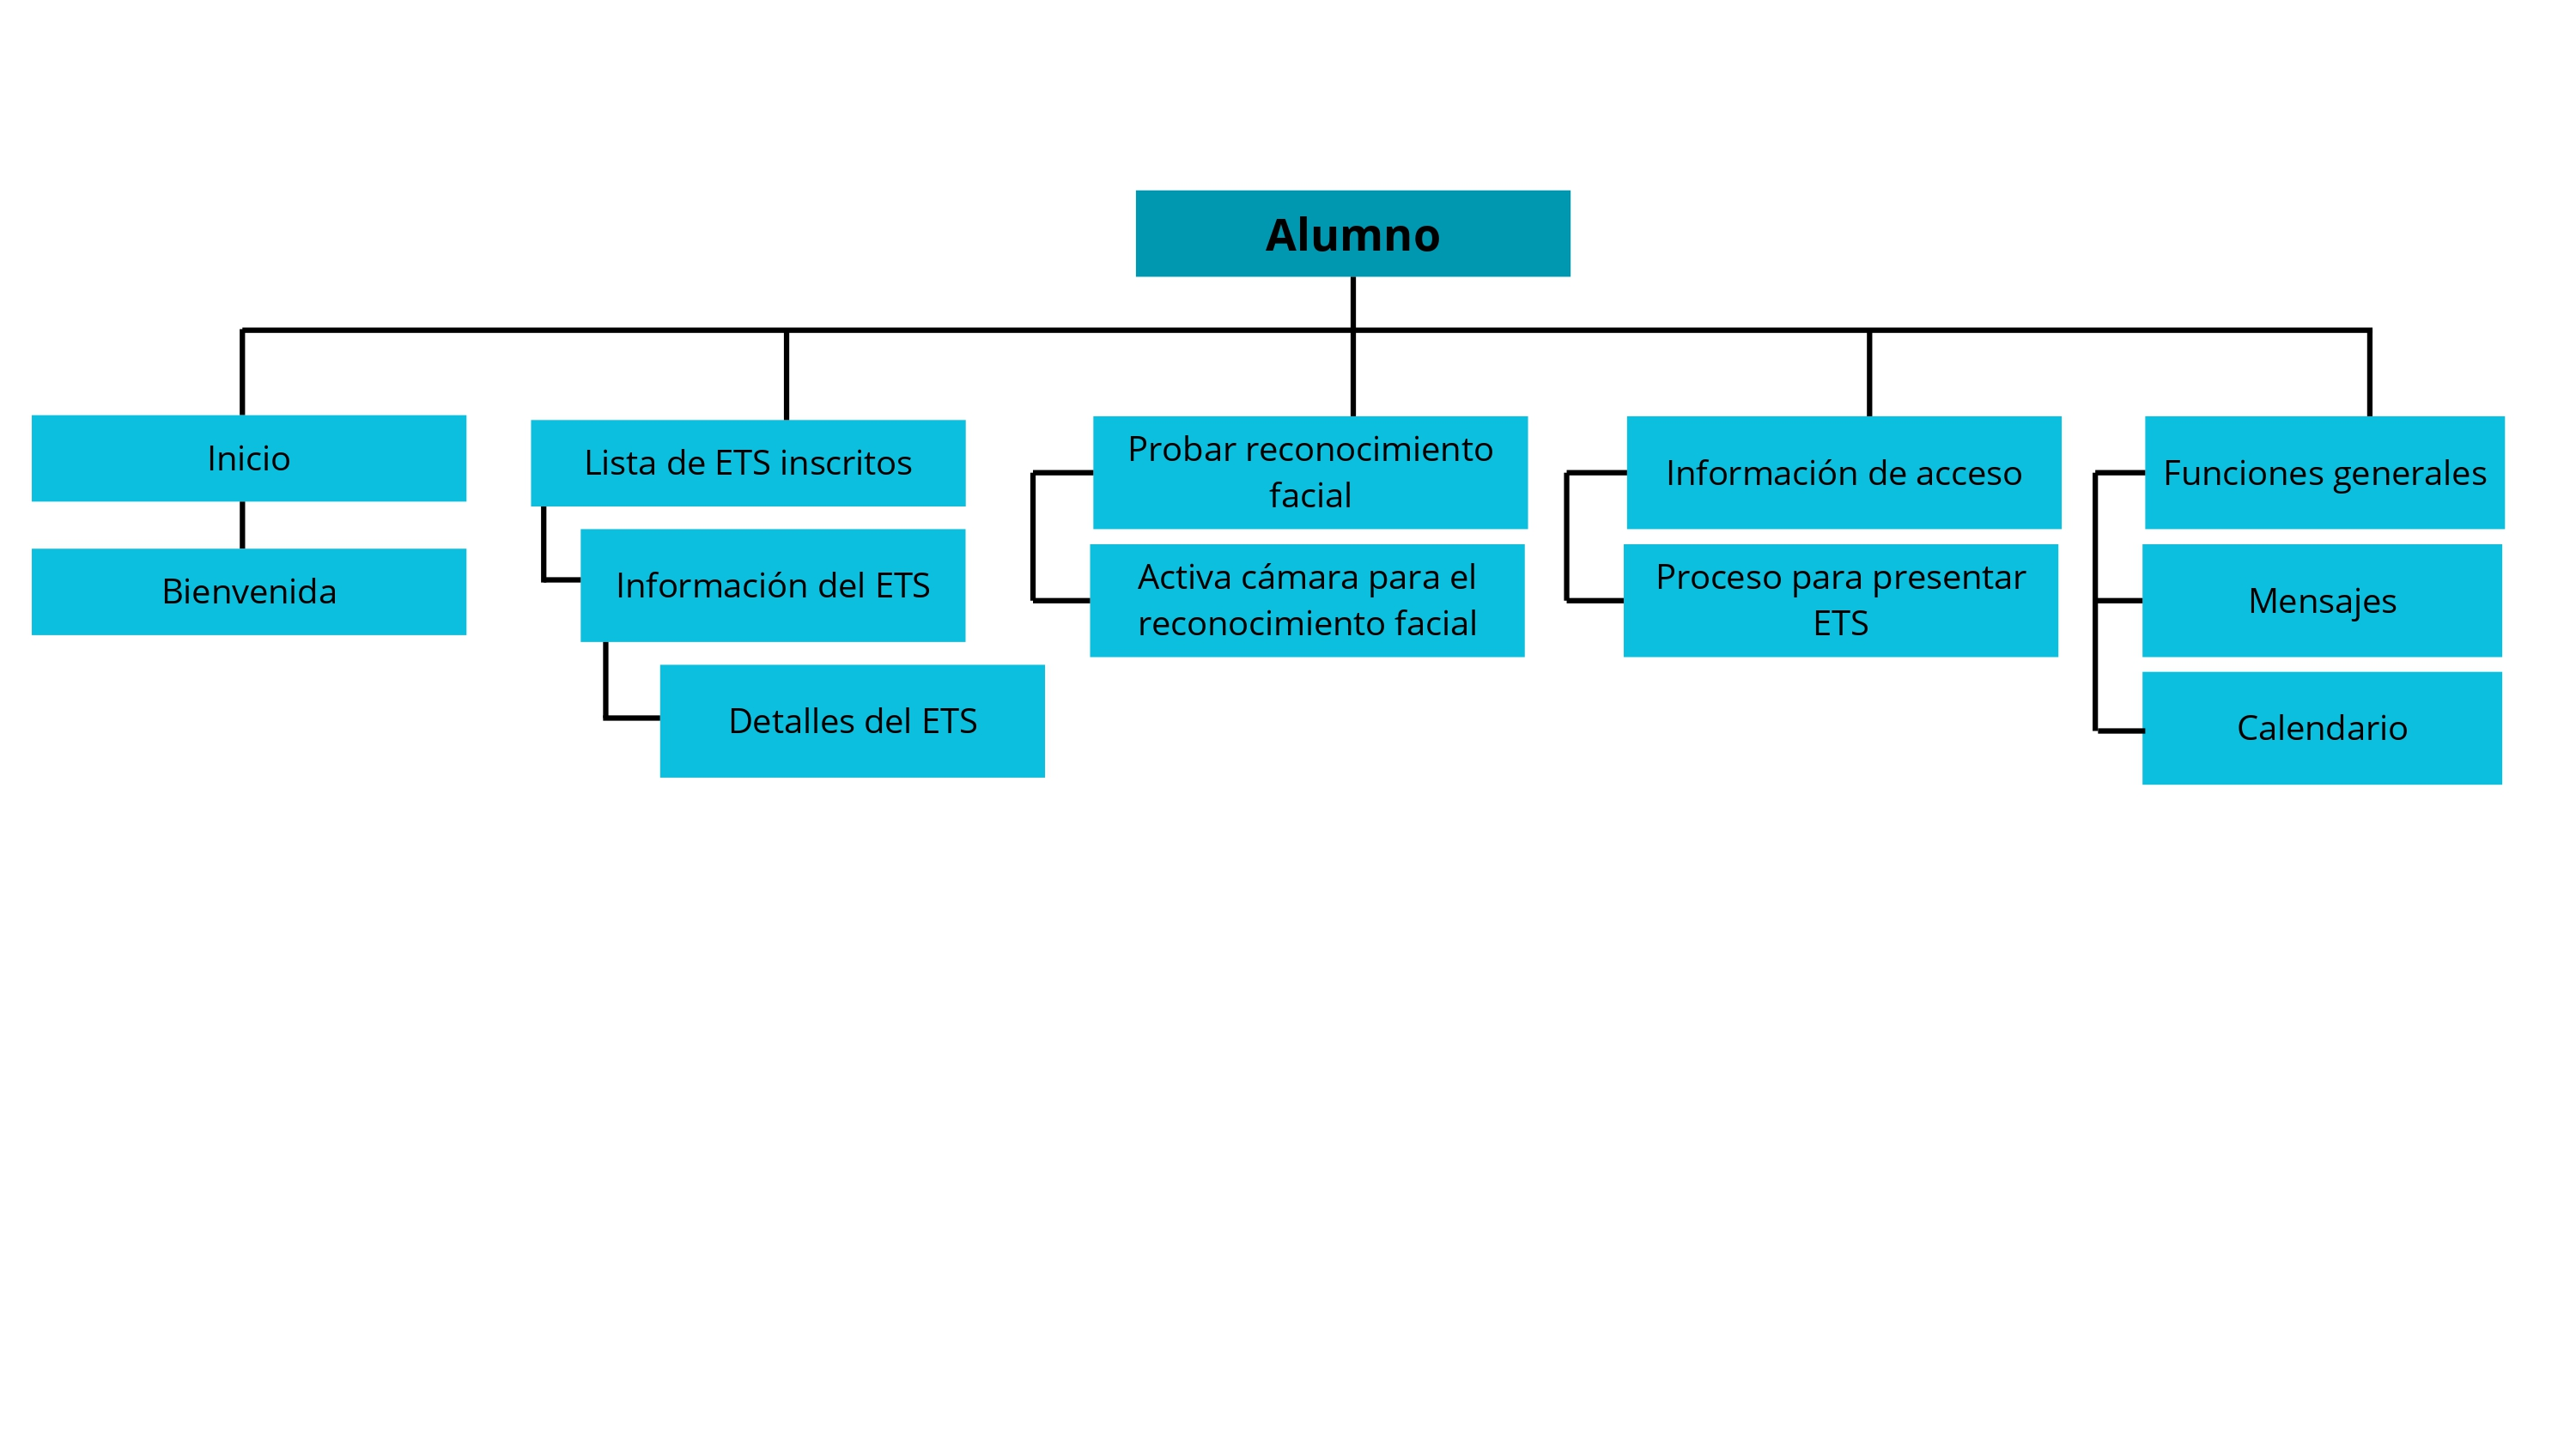
\includegraphics[width=1.0\textwidth]{images/alumno}
			\caption{Mapa de navegación del alumno}
			\label{fig:Mapa de navegación del alumno}
		\end{center}
\end{figure}

\clearpage

\begin{figure}[htbp]
	\begin{center}
		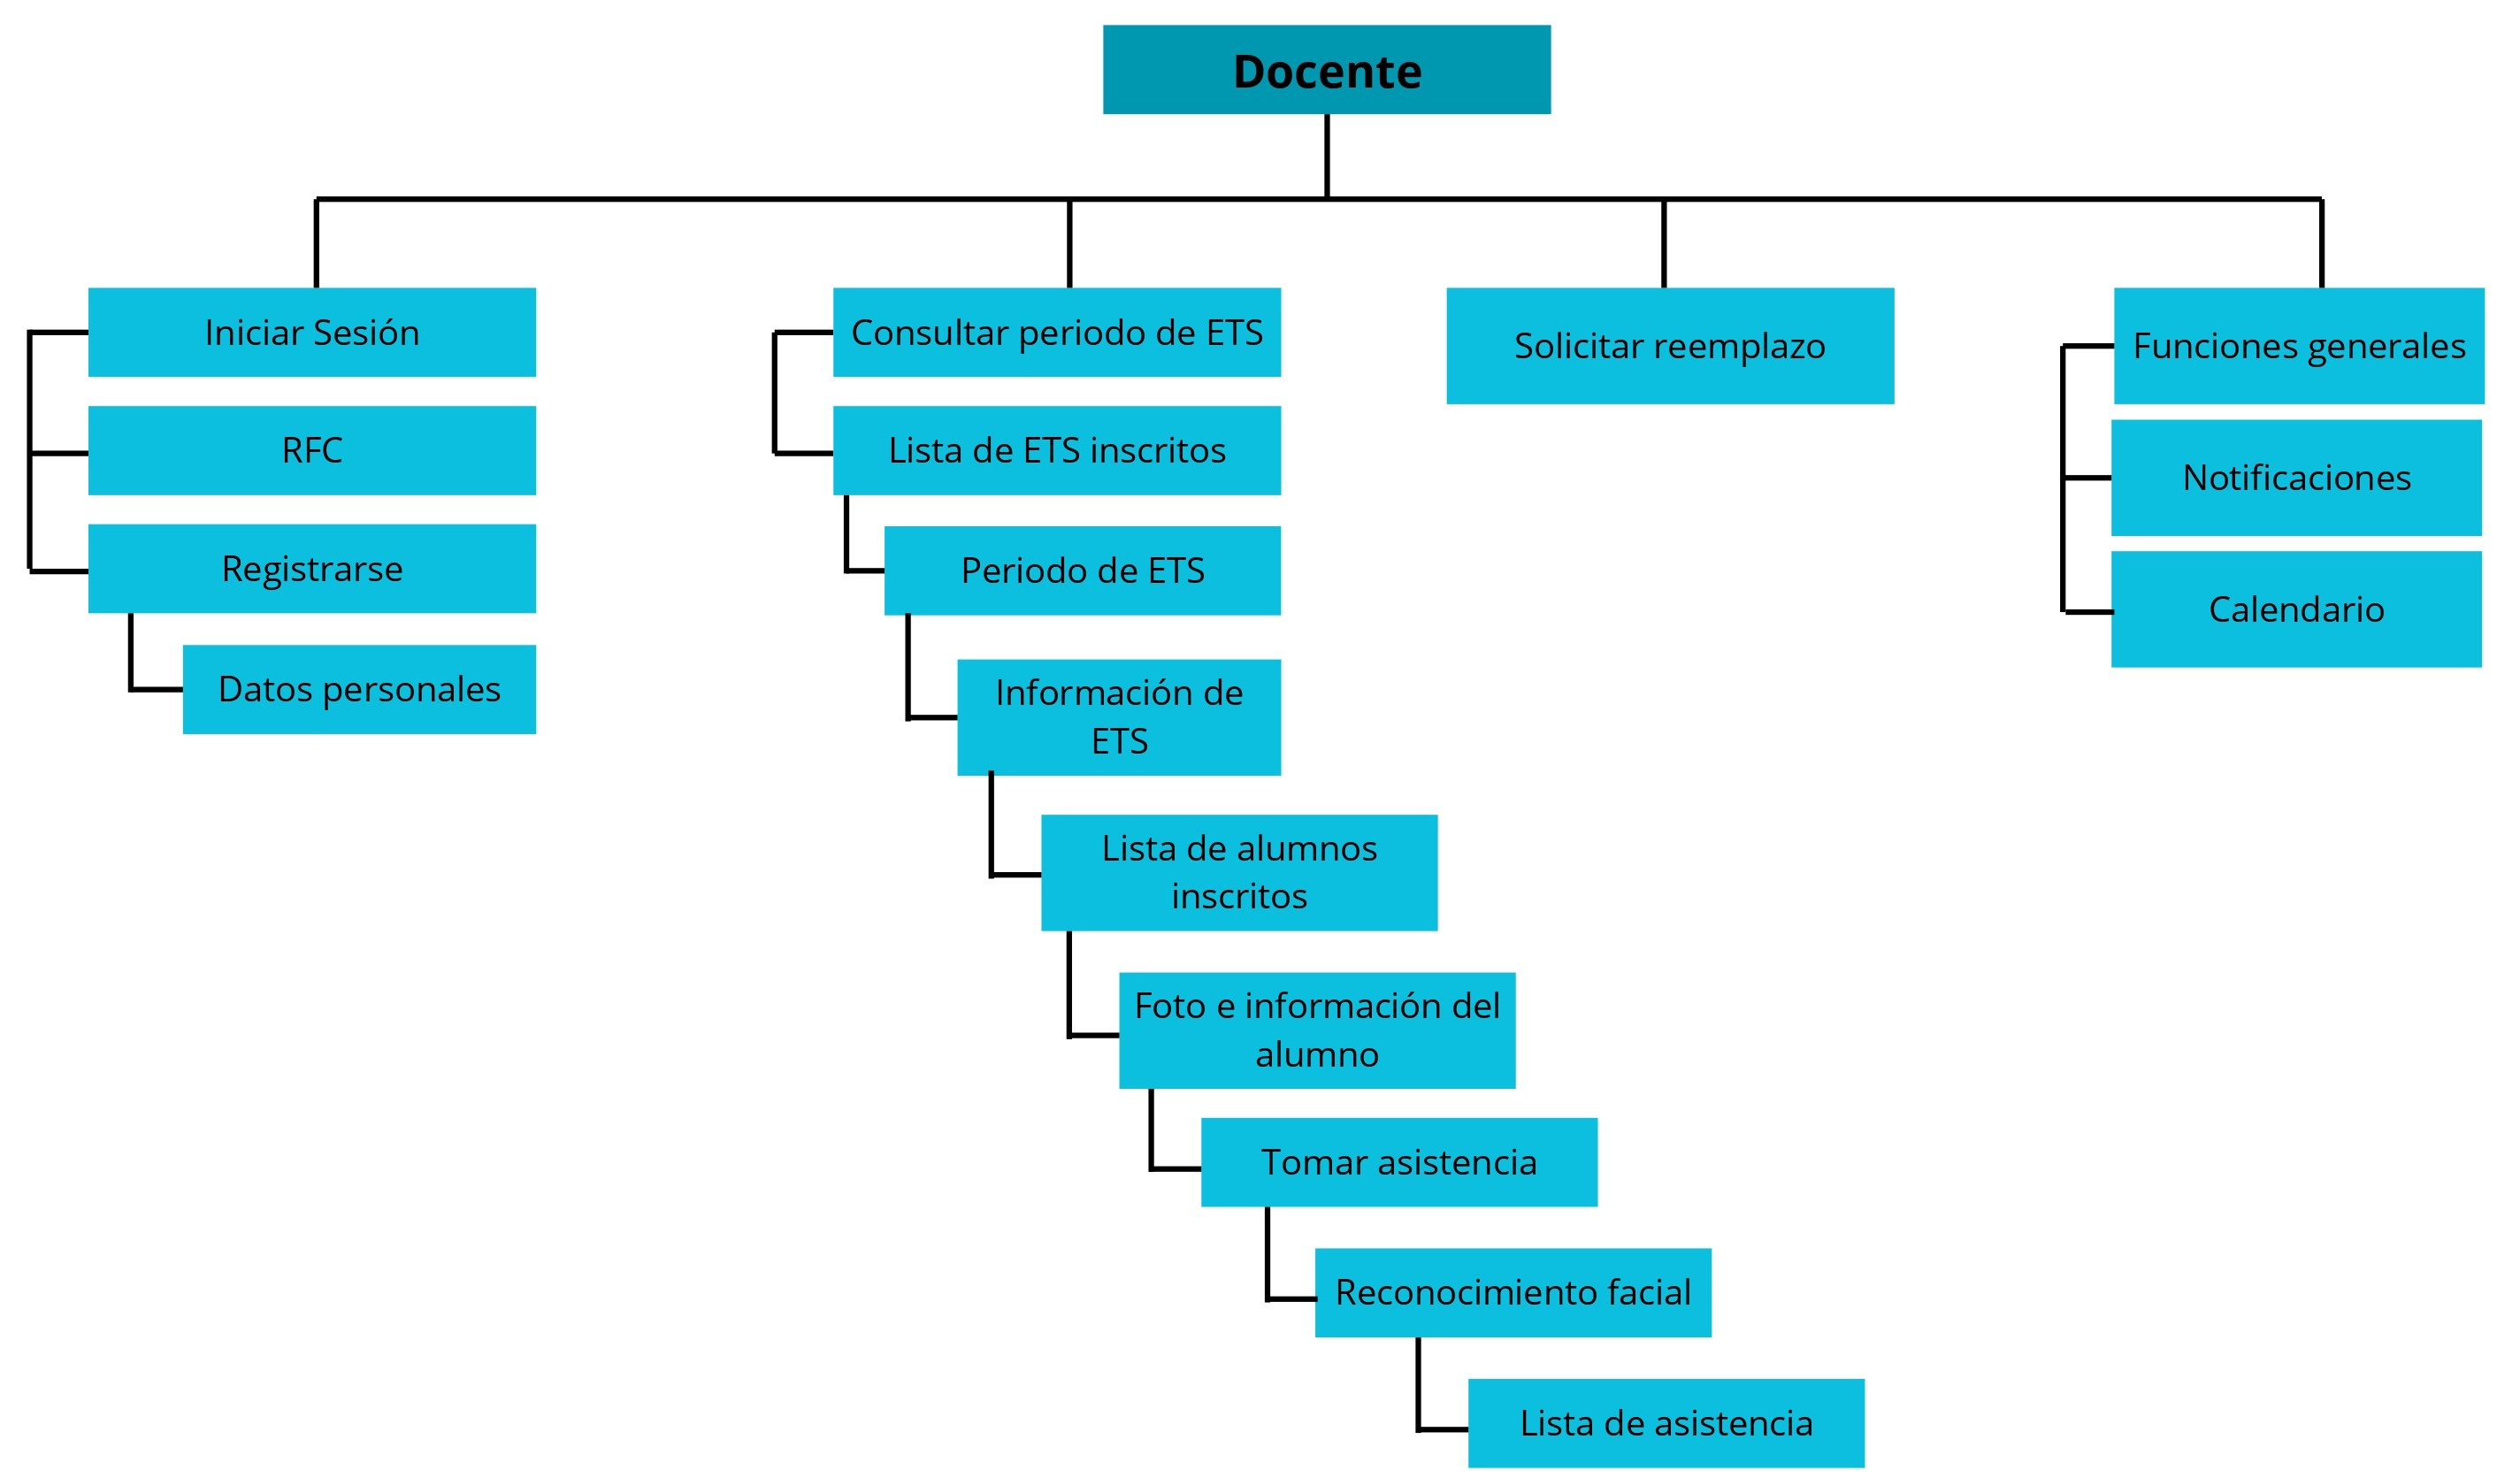
\includegraphics[width=1.0\textwidth]{images/docente}
		\caption{Mapa de navegación del docente}
		\label{fig:Mapa de navegación del docente}
	\end{center}
\end{figure}

\clearpage

\begin{figure}[htbp]
	\begin{center}
		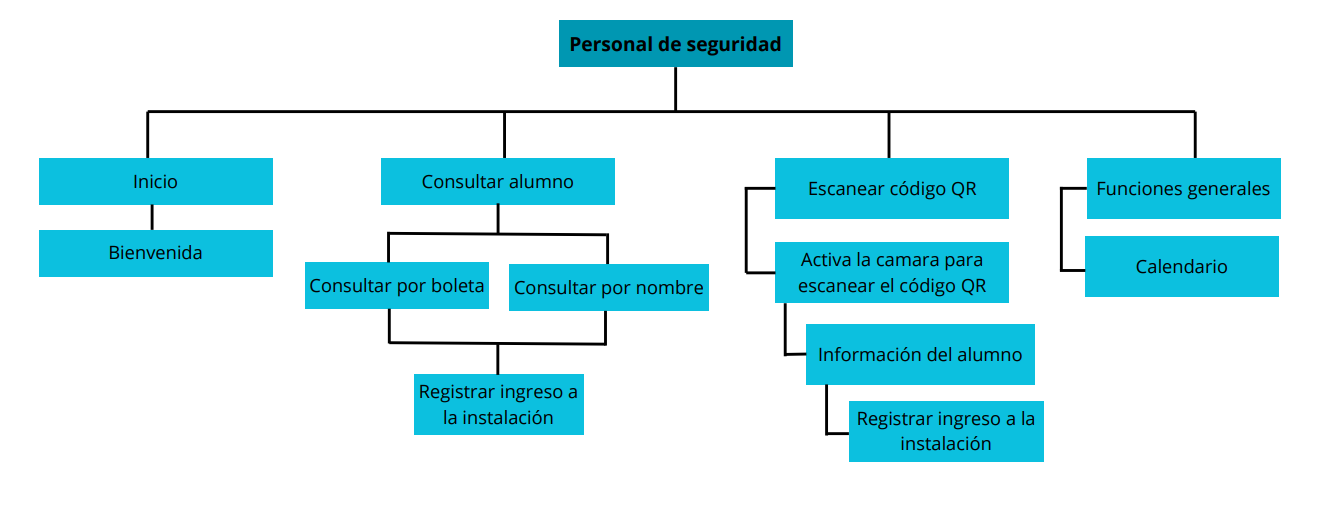
\includegraphics[width=.9\textwidth]{images/personalseguridad}
		\caption{Mapa de navegación del personal de seguridad}
		\label{fig:Mapa de navegación del personal de seguridad}
	\end{center}
\end{figure}

\newpage
% !TeX root = ../ejemplo.tex

%--------------------------------------
\subsection{IU01: Pantalla Iniciar sesión del sistema móvil}

\IUfig[.40]{UI-CU01}{IU01}{Pantalla Iniciar sesión del sistema móvil.}

\newpage

\subsubsection{Objetivo}
Controlar el acceso al sistema móvil, permitiendo a los usuarios registrados (docentes, personal de seguridad, alumnos, presidentes de academia y jefes de departamento) autenticarse mediante sus credenciales correspondientes.

\subsubsection{Diseño}
Esta pantalla \IUref{IU01}{Pantalla Iniciar sesión del sistema móvil} (ver figura~\ref{IU01}) es la primera que se muestra al iniciar la aplicación. Permite a los diferentes tipos de usuarios ingresar sus datos de autenticación.



La pantalla contiene los siguientes elementos:
\begin{itemize}
	\item \textbf{Título:} "Iniciar sesión".
	\item \textbf{Campo "Boleta":} Para que los alumnos ingresen su número de boleta. Tiene un icono de usuario asociado.
	\item \textbf{Campo "Contraseña":} Para que todos los usuarios ingresen su contraseña. Tiene un icono de candado asociado.
	\item \textbf{Botón \IUbutton{Entrar}:} Permite iniciar la sesión una vez que se han introducido las credenciales.
\end{itemize}

\subsubsection{Salidas}
Redirección a la pantalla de saludo correspondiente al rol del usuario autenticado, mostrando un saludo y su nombre. Las posibles pantallas de saludo son:
\begin{itemize}
	\item \IUref{IUE01}{Pantalla de saludo del docente} (para docentes, presidentes de academia y jefes de departamento).
	\item \IUref{IUE02}{Pantalla de saludo del personal de seguridad}.
	\item \IUref{IUE03}{Pantalla de saludo del alumno}.
	\item \IUref{IUE06}{Pantalla de saludo del presidente de academia/jefe de departamento} (también para presidentes de academia y jefes de departamento).
\end{itemize}

\subsubsection{Entradas}
Dependiendo del rol del usuario:
\begin{itemize}
	\item \textbf{Alumno:} Número de boleta y Contraseña.
	\item \textbf{Personal de seguridad:} CURP y Contraseña.
	\item \textbf{Docente, Presidente de academia, Jefe de departamento:} RFC y Contraseña.
\end{itemize}
	
	\subsubsection{Comandos}
	\begin{itemize}
		\item \IUbutton{Entrar}:
		\begin{enumerate}
			\item Verifica que se hayan llenado todos los campos (Boleta y Contraseña). Si falta algún campo, muestra el mensaje \textbf{\hyperref[msg:CU01-E1]{MSG-CU01-E1}}{``Por favor, completa todos los campos.''}.
			\item Verifica que las credenciales (Boleta y Contraseña) coincidan con un usuario registrado en el sistema. Si no coinciden, muestra el mensaje \textbf{\hyperref[msg:CU01-E2]{MSG-CU01-E2}} ``Datos incorrectos.''.
			\item En caso de pérdida de conexión durante la verificación, muestra el mensaje \textbf{\hyperref[msg:CU01-E3]{MSG-CU01-E3}} ``Conexión perdida.''.
			\item Si la autenticación es exitosa, determina el rol del usuario y lo redirige a la pantalla de saludo correspondiente (\IUref{IUE01}{Pantalla de saludo del docente}, \IUref{IUE02}{Pantalla de saludo del personal de seguridad}, \IUref{IUE03}{Pantalla de saludo del alumno} o \IUref{IUE06}{Pantalla de saludo del presidente de academia/jefe de departamento}).
		\end{enumerate}
		
	\end{itemize}
	
	\subsubsection{Mensajes}
	\begin{itemize}
		\item \textbf{\hyperref[msg:CU01-E1]{MSG-CU01-E1}} Por favor, completa todos los campos.
		\item \textbf{\hyperref[msg:CU01-E2]{MSG-CU01-E2}} Datos incorrectos.
		\item \textbf{\hyperref[msg:CU01-E3]{MSG-CU01-E3}} Conexión perdida.
	\end{itemize}



\newpage

% !TeX root = ../ejemplo2.tex

%--------------------------------------
\subsection{IU02: Pantalla Consultar calendario escolar}

\IUfig[.40]{UI-CU02}{IU02}{Pantalla Consultar calendario escolar.}

\newpage

\subsubsection{Objetivo}
Permitir a los usuarios visualizar el calendario escolar y obtener información sobre el tiempo restante para el inicio del próximo periodo de ETS.

\subsubsection{Diseño}
Esta pantalla \IUref{IU02}{Pantalla Consultar calendario escolar} (ver figura~\ref{IU02}) muestra el calendario escolar actual. Se puede acceder a ella mediante el botón con forma de calendario que está visible en la barra de navegación inferior, presente en la mayoría de las pantallas de la aplicación (excepto la de inicio de sesión).



La pantalla contiene los siguientes elementos:
\begin{itemize}
	\item \textbf{Barra de navegación superior:}
	\begin{itemize}
		\item \textbf{Icono de flecha hacia la izquierda:} Para regresar a la pantalla anterior.
		\item \textbf{Título:} Calendario Escolar.
		\item \textbf{Icono de tres puntos horizontales con una burbuja de diálogo:} Accede a la funcionalidad de mensajes dentro de la aplicación
	\end{itemize}
	\item \textbf{Imagen del Calendario Escolar:} Visualización del calendario académico actual.
	\item \textbf{Botón \IUbutton{Calcular cuántos días faltan para el periodo de ETS}:} Al presionarlo, el sistema calcula y muestra el tiempo restante para el próximo periodo de ETS.
	\item \textbf{Barra de navegación inferior:} Contiene iconos para:
	\begin{itemize}
		\item \textbf{Icono de casa:} Redirección a la pantalla de saludo correspondiente al usuario.
		\item \textbf{Icono de campana:} Redirección a la pantalla de notificaciones.
		\item \textbf{Icono de calendario con marcas:} Indica la pantalla actual del calendario.
		\item \textbf{Icono de flecha apuntando hacia la derecha saliendo de un recuadro:} Función de cerrar sesión.
	\end{itemize}
\end{itemize}

\subsubsection{Salidas}
Muestra un mensaje indicando cuántos días faltan para el periodo de ETS o si actualmente es periodo de ETS, en respuesta a la acción del botón \IUbutton{Calcular cuántos días faltan para el periodo de ETS}.

\subsubsection{Entradas}
Ninguna directa por parte del usuario en esta pantalla, más allá de la interacción con los botones.

\subsubsection{Comandos}
\begin{itemize}
	\item \IUbutton{Calcular cuántos días faltan para el periodo de ETS}:
	\begin{enumerate}
		\item Recupera la fecha de inicio del próximo periodo de ETS registrada en el sistema.
		\item Calcula la diferencia en días entre la fecha actual y la fecha de inicio del próximo periodo de ETS.
		\item Si la fecha de inicio es posterior a la actual, muestra el mensaje \textbf{ ``Faltan (cantidad de días) días para el periodo de ETS.''}
		\item Si la fecha de inicio es igual o anterior a la actual, muestra el mensaje \textbf{ ``Actualmente es periodo de ETS.''}
		\item En caso de que no se haya registrado el siguiente periodo de ETS, muestra el mensaje \textbf{ ``Aún no está registrado el siguiente periodo de ETS.''}
		\item En caso de pérdida de conexión, muestra el mensaje \textbf{ ``Conexión perdida.''}
	\end{enumerate}
	\item \textbf{Icono de campana (barra de navegación inferior):} Redirige a la pantalla \IUref{UI03}{Consultar notificaciones}.
	\item \textbf{Icono de casa (barra de navegación inferior):} Redirige a la pantalla de menú correspondiente al tipo de usuario.
	\item \textbf{Icono de flecha saliendo (barra de navegación inferior):} Función de cerrar sesión.
	\item \textbf{Icono de flecha izquierda (barra superior):} Regresa a la pantalla anterior.
	\item \textbf{Icono de tres puntos horizontales con una burbuja de diálogo:} Accede a la funcionalidad de mensajes dentro de la aplicación.
\end{itemize}

\subsubsection{Mensajes}

\begin{itemize}
	\item \textbf{ Faltan (cantidad de días) días para el periodo de ETS.}
	\item \textbf{ Actualmente es periodo de ETS.}
	\item \textbf{ Aún no está registrado el siguiente periodo de ETS.}
	\item \textbf{ Conexión perdida.}
\end{itemize}


\newpage

% !TeX root = ../ejemplo.tex

%--------------------------------------
\subsection{IU03 Pantalla Consultar notificaciones}

\subsubsection{Objetivo}
Permitir que los usuarios puedan gestionar sus notificaciones y marcarlas como leidas.
\subsubsection{Diseño}
    Esta pantalla \IUref{IU03}{Pantalla Consultar notificaciones } (ver figura~\ref{IU03}) puede ser accedida desde cualquier otra pantalla que no sea el inicio de sesión mediante el botón con forma de campana.
\IUfig[.35]{UI-CU03}{IU03}{Pantalla Consultar notificaciones.}

\subsubsection{Salidas}
Menciona que la notificación seleccionada ha sido establecida como leída.
\subsubsection{Entradas}
   Ninguna.

\subsubsection{Comandos}
\begin{itemize}
    \item \IUbutton{Botón con palomita} toma la notificación seleccionada y la marca como leída.
    \item \IUbutton{Buscador} En este buscador se puede buscar las notificaciones por fecha.
    \item \IUbutton{Calendario} Redirige a la pantalla \IUref{UI02}{Consultar calendario escolar}.
    \item \IUbutton{Home} Redirige a la pantalla de bienvenida correspondiente al tipo de usuario.
\end{itemize}

\subsubsection{Mensajes}
     
\begin{Citemize}
    \item {\bf MSG-8}{``Actualmente no hay notificaciones.}
\end{Citemize}



\newpage

%--------------------------------------
\subsection{IU04 Pantalla Periodo de ETS}

\subsubsection{Objetivo}
	Permitir al docente consultar los periodos de ETS que le han sido asignados. 

\subsubsection{Diseño}
	Esta pantalla \IUref{IU04}{Pantalla Periodo de ETS} (ver figura~\ref{IU04}) aparece luego de seleccionar la opción de Consultar Periodos de ETS de la pantalla principal. 

\IUfig[.35]{cu04}{IU04}{Pantalla Periodo de ETS.}

\subsubsection{Salidas}

	Lista de periodos de ETS asignados. 

\subsubsection{Entradas}
Ninguna

\subsubsection{Comandos}

\begin{Citemize}
	\item \IUbutton{Calendario} Redirige a la pantalla \IUref{UI02}{Consultar calendario escolar}.
	\item \IUbutton{Campana} Redirige a la pantalla \IUref{UI03}{Consultar notificaciones }.
	\item \IUbutton{Home} Redirige a la pantalla de bienvenida correspondiente al tipo de usuario.
	\item \IUbutton{Periodo de ETS} Selecciona un periodo de ETS y lo redirige a la \IUref{IU04}{pantalla Periodo de ETS}. 
\end{Citemize}


\subsubsection{Mensajes}

\begin{Citemize}
	\item {\bf MSG-9}{``Error al consultar la base de datos. Intente nuevamente más tarde''.}
	\item {\bf MSG-10}{``No tienes periodos de ETS asignados.''}
\end{Citemize}


\newpage

%--------------------------------------
\subsection{IU05 Pantalla Consultar ETS}

\subsubsection{Objetivo}
	Permitir al docente consultar los ETS que tiene asignados. 

\subsubsection{Diseño}
	Esta pantalla \IUref{IU05}{Pantalla Consultar ETS} (ver figura~\ref{IU05}) aparece luego de seleccionar un periodo de ETS. 

\IUfig[.35]{cu05}{IU05}{Pantalla Consultar ETS.}

\subsubsection{Salidas}
	Lista de ETS asignados. 

\subsubsection{Entradas}
	Ninguna
	
\subsubsection{Comandos}
\begin{Citemize}

	\item \IUbutton{Calendario} Redirige a la pantalla \IUref{UI02}{Consultar calendario escolar}.
	\item \IUbutton{Campana} Redirige a la pantalla \IUref{UI03}{Consultar notificaciones }.
	\item \IUbutton{Home} Redirige a la pantalla de bienvenida correspondiente al tipo de usuario.
	\item \IUbutton{ETS} Selecciona un ETS y lo redirige a la \IUref{IU06}{pantalla Información de ETS}.
\end{Citemize}

\subsubsection{Mensajes}

\begin{Citemize}
	\item {\bf MSG-9}{``Error al consultar la base de datos. Intente nuevamente más tarde.''.}
	\item {\bf MSG-11}{``No hay ETS asignados actualmente.''}
\end{Citemize}


\newpage

%--------------------------------------
\subsection{IU06: Pantalla Información de ETS}

\IUfig[.40]{cu06}{IU06}{Pantalla Información de ETS}
\newpage

\subsubsection{Objetivo}
Permitir al docente visualizar la información detallada cada ETS que tiene asignado.

\subsubsection{Diseño}
Esta pantalla \IUref{IU06}{Pantalla Información de ETS} (ver figura~\ref{IU06}) aparece luego de seleccionar un ETS asignado.



La pantalla contiene los siguientes elementos:
\begin{itemize}
	\item \textbf{Barra de navegación superior:}
	\begin{itemize}
		\item \textbf{Icono de flecha hacia la izquierda:} Para regresar a la pantalla anterior (\IUref{IU05}{Pantalla Consultar ETS}).
		\item \textbf{Título:} "Detalles del ETS de Bases de Datos".
		\item \textbf{Icono de tres puntos horizontales con una burbuja de diálogo:} Accede a la funcionalidad de mensajes dentro de la aplicación.
	\end{itemize}
	\item \textbf{Información del ETS:} Muestra los detalles del ETS en forma de lista o texto informativo:
	\begin{itemize}
		\item Unidad de aprendizaje.
		\item Tipo de ETS.
		\item Periodo.
		\item Fecha de aplicación.
		\item Turno.
		\item Duración.
		\item Salones asignados:
		\item Hora de inicio.
	\end{itemize}
	\item \textbf{Botón \IUbutton{Solicitar reemplazo}:} Visible si el docente es el aplicador del ETS. Redirige a la \IUref{IU07}{Pantalla Solicitar remplazo}.
	\item \textbf{Botón \IUbutton{Ir a la lista de alumnos}:} Visible si hay alumnos inscritos en el ETS. Redirige a la \IUref{IU08}{Pantalla Lista de alumnos inscritos a un ETS}.
	\item \textbf{Barra de navegación inferior:} Contiene iconos para:
	\begin{itemize}
		\item \textbf{Icono de casa:} Redirección a la pantalla de saludo correspondiente al tipo de usuario.
		\item \textbf{Icono de campana:} Redirección a la pantalla de notificaciones.
		\item \textbf{Icono de calendario con marcas:} Redirección a la pantalla \IUref{IU02}{Consultar calendario escolar}.
		\item \textbf{Icono de flecha apuntando hacia la derecha saliendo de un recuadro:} Cierra la sesión del usuario y lo regresa a la pantalla de inicio de sesión (\IUref{IU01}{Iniciar sesión del sistema móvil}).
	\end{itemize}
\end{itemize}

\subsubsection{Salidas}
Información detallada del ETS seleccionado.

\subsubsection{Entradas}
Ninguna

\subsubsection{Comandos}
\begin{itemize}
	\item \IUbutton{Solicitar reemplazo}: Redirige a la pantalla \IUref{IU07}{Solicitar remplazo}.
	\item \IUbutton{Ir a la lista de alumnos}: Redirige a la pantalla \IUref{IU08}{Lista de alumnos inscritos a un ETS}.
	\item \textbf{Icono de flecha izquierda (barra superior):} Regresa a la pantalla anterior (\IUref{IU05}{Pantalla Consultar ETS}).
	\item \textbf{Icono de tres puntos (barra superior):} Accede a la funcionalidad de mensajes dentro de la aplicación.
	\item \textbf{Icono de calendario (barra de navegación inferior):} Redirige a la pantalla \IUref{IU02}{Consultar calendario escolar}.
	\item \textbf{Icono de campana (barra de navegación inferior):} Redirige a la pantalla de notificaciones.
	\item \textbf{Icono de casa (barra de navegación inferior):} Redirección a la pantalla de saludo correspondiente al tipo de usuario.
	\item \textbf{Icono de flecha saliendo (barra de navegación inferior):} Cierra la sesión del usuario y lo regresa a la pantalla de inicio de sesión (\IUref{IU01}{Iniciar sesión del sistema móvil}).
\end{itemize}

\subsubsection{Mensajes}
\begin{itemize}
	\item \textbf{Ocurrió un error al desplegar los detalles del ETS.}
	\item \textbf{Error al consultar la base de datos. Intente nuevamente más tarde.}
\end{itemize}


\newpage

%--------------------------------------
\subsection{IU07: Pantalla de Solicitar remplazo}

\subsubsection{Objetivo}
Permitir al docente pedir que otro docente lo remplaze en la aplicacion de un ETS.

\subsubsection{Diseño}
Esta pantalla \IUref{IU07}{Pantalla de Solicitar remplazo} (ver figura~\ref{IU07}) aparece luego de que el docente presione el boton \IUbutton{Solicitar reemplazo} en la pantalla \IUref{IU06}{Pantalla Información de ETS}.

\IUfig[.35]{UI-CU43}{IU07}{Pantalla de Solicitar remplazo}

\subsubsection{Salidas}
Confirmación de envio de solicitud

\subsubsection{Entradas}
Identificador del ETS y razon por la que se pide el remplazo.

\subsubsection{Comandos}
\begin{itemize}
	\item \IUbutton{Enviar solicitud}: Permite enviar la notificación al jefe de departamento y/o al presidente de academia para pedir el remplazo.
	\item \IUbutton{Calendario} Redirige a la pantalla \IUref{UI02}{Consultar calendario escolar}.
    \item \IUbutton{Campana} Redirige a la pantalla \IUref{UI03}{Consultar notificaciones }.
    \item \IUbutton{Home} Redirige a la pantalla de bienvenida correspondiente al tipo de usuario.
\end{itemize}

\subsubsection{Mensajes}

\begin{itemize}
	\item \textbf{ ``Solicitud exitosa. La solicitud de reemplazo ha sido registrada correctamente''}
	\item \textbf{ ``Ya existe una solicitud pendiente para este ETS'', indicando que ya se ha realizado una solicitud previa para el ETS".}
\end{itemize}


\newpage

%--------------------------------------
\subsection{IU08: Pantalla Lista de asistencia de ETS}

\IUfig[.40]{cu08}{IU08}{Pantalla Lista de asistencia de ETS}
\newpage

\subsubsection{Objetivo}
Permitir al docente visualizar la lista de los alumnos inscritos en un ETS asignado, junto con su estado de asistencia, y acceder a las funciones de reporte dentro del periodo permitido.

\subsubsection{Diseño}
Esta pantalla \IUref{IU08}{Pantalla Lista de asistencia de ETS} (ver figura~\ref{IU08}) muestra la lista de alumnos inscritos en el ETS seleccionado. Se accede a ella al presionar el botón "Ir a la lista de alumnos"  desde la \IUref{IU06}{Pantalla Información de ETS}.



La pantalla contiene los siguientes elementos:
\begin{itemize}
	\item \textbf{Barra de navegación superior:}
	\begin{itemize}
		\item \textbf{Icono de flecha hacia la izquierda:} Para regresar a la pantalla anterior (\IUref{IU06}{Pantalla Información de ETS}).
		\item \textbf{Título:} ETS de Bases de Datos\newline 25/2\newline Lista de alumnos inscritos.
		\item \textbf{Icono de tres puntos horizontales con una burbuja de diálogo:} Accede a la funcionalidad de mensajes dentro de la aplicación.
	\end{itemize}
	\item \textbf{Lista de alumnos inscritos:} Muestra a los alumnos inscritos en el ETS en forma de tarjetas o filas. Para cada alumno se muestra:
	\begin{itemize}
		\item \textbf{Boleta y Nombre:} Presentados como texto. Este elemento, al ser presionado (si está habilitado), redirige a la \textbf{Pantalla Reporte} (\IUref{IUE07}{Creación del reporte}).
		\item \textbf{Icono de estado de asistencia:} Un icono visual que representa el estado de asistencia del alumno (ej., una "X" roja o una paloma verde). Al presionarlo, redirige a la \IUref{IU20}{Pantalla mostrar la foto e información del alumno} (solo dentro del periodo de tiempo especificado).
	\end{itemize}
	\item \textbf{Barra de navegación inferior:} Contiene iconos para:
	\begin{itemize}
		\item \textbf{Icono de casa:} Redirección a la pantalla de saludo correspondiente al tipo de usuario.
		\item \textbf{Icono de campana:} Redirección a la pantalla de notificaciones.
		\item \textbf{Icono de calendario con marcas:} Redirección a la pantalla \IUref{IU02}{Consultar calendario escolar}.
		\item \textbf{Icono de flecha apuntando hacia la derecha saliendo de un recuadro:} Cierra la sesión del usuario y lo regresa a la pantalla de inicio de sesión (\IUref{IU01}{Iniciar sesión del sistema móvil}).
	\end{itemize}
\end{itemize}

\subsubsection{Salidas}
Muestra la lista de los alumnos inscritos en el ETS, incluyendo su boleta, nombre y un icono de estado de asistencia. Puede mostrar mensajes informativos sobre el periodo de reporte y los permisos del docente.

\subsubsection{Entradas}
Ninguna directa por parte del usuario en esta pantalla, ya que la lista se muestra al acceder a ella.

\subsubsection{Comandos}
\begin{itemize}
	\item \textbf{Boleta y Nombre del alumno (al ser presionado):} Si está habilitado (dentro del periodo de reporte y si el docente tiene permisos), redirige a la \textbf{Pantalla Reporte} (\IUref{IUE07}{Creación del reporte}).
	\item \textbf{Icono de estado de asistencia (al ser presionado):} Redirige a la \IUref{IU20}{Pantalla mostrar la foto e información del alumno} (solo dentro del periodo de tiempo especificado).
	\item \textbf{Icono de calendario (barra de navegación inferior):} Redirige a la pantalla \IUref{IU02}{Consultar calendario escolar}.
	\item \textbf{Icono de campana (barra de navegación inferior):} Redirige a la pantalla de notificaciones.
	\item \textbf{Icono de casa (barra de navegación inferior):} Redirección a la pantalla de saludo correspondiente al tipo de usuario.
	\item \textbf{Icono de flecha saliendo (barra de navegación inferior):} Cierra la sesión del usuario y lo regresa a la pantalla de inicio de sesión (\IUref{IU01}{Iniciar sesión del sistema móvil}).
	\item \textbf{Icono de flecha izquierda (barra superior):} Regresa a la pantalla anterior (\IUref{IU06}{Pantalla Información de ETS}).
	\item \textbf{Icono de tres puntos (barra superior):} Accede a la funcionalidad de mensajes dentro de la aplicación.
\end{itemize}

\subsubsection{Mensajes}
\begin{itemize}
	\item \textbf{\hyperref[msg:CU08-E2]{MSG-CU08-E2}} Error al consultar la base de datos. Intente nuevamente más tarde.
	\item \textbf{\hyperref[msg:CU08-A1]{MSG-CU08-A1}} No hay alumnos inscritos al ETS.
	\item \textbf{\hyperref[msg:CU08-C1]{MSG-CU08-C1}} El ETS seleccionado no es válido.
	\item \textbf{\hyperref[msg:CU08-D1]{MSG-CU08-D1}} Aún no es periodo para crear los reportes. Faltan (tiempo).
	\item \textbf{\hyperref[msg:CU08-ET2]{MSG-CU08-ET2}} El periodo para registrar los reportes ha concluido.
	\item \textbf{\hyperref[msg:CU08-F1]{MSG-CU08-F1}} Usted no está autorizado para crear el reporte de este alumno.
\end{itemize}
\newpage

%--------------------------------------
\subsection{IU09 Asignar docente de remplazo}

\subsubsection{Objetivo}
Permitir al jefe de departamento y/o al presidente de academia responder a las solicitudes de remplazo y asignar un docente de remplazo para el ETS especifico.

\subsubsection{Diseño}
Esta pantalla \IUref{IU09}{Asignar docente de remplazo} (ver figura~\ref{IU09}) aparece luego de que el jefe de departamento y/o al presidente de academia revisen sus notificaciones y seleccione una solicitud de remplazo.

\IUfig[.35]{UI-CU44}{IU09}{Pantalla de Asignar docente de remplazo}

\subsubsection{Salidas}
Confirmación de asignación del nuevo docente y se muestra el mensaje {\bf MSG-42}{``docente de remplazo asignado con exito.''}.

\subsubsection{Entradas}
Identificador del ETS y nombre del nuevo docente asignado.

\subsubsection{Comandos}
\begin{itemize}
	\item \IUbutton{Asignar}: Permite enviar la notificación docente de que su remplzado ha sido asignado y ademas asigna el remplazo como docente aplicador en el sistema.
\end{itemize}

\subsubsection{Mensajes}

\begin{Citemize}
	\item {\bf MSG-28} {``El proceso no se pudo realizar por un fallo de red''.}
	\item {\bf MSG-42}{``docente de remplazo asignado con exito'.'}
\end{Citemize}



\newpage


%--------------------------------------
\subsection{IU10 Pantalla Código QR}

\subsubsection{Objetivo}
Permitir al personal de seguridad escanear el código QR de la credencial del alumno.

\subsubsection{Diseño}
Esta pantalla \IUref{IU10}{Pantalla Código QR} (ver figura~\ref{IU10}) aparece una vez que el personal de seguridad inicia sesión. 

\IUfig[.35]{cu12}{IU10}{Pantalla Código QR}

\subsubsection{Salidas}
Información del alumno

\subsubsection{Entradas}
Ninguna

\subsubsection{Comandos}
\begin{itemize}
	\item \IUbutton{Escanear}: Permite escanear el código QR de la credencial del alumno.
	\item \IUbutton{Calendario} Redirige a la pantalla \IUref{UI02}{Consultar calendario escolar}.
    \item \IUbutton{Campana} Redirige a la pantalla \IUref{UI03}{Consultar notificaciones }.
    \item \IUbutton{Home} Redirige a la pantalla de bienvenida correspondiente al tipo de usuario.
\end{itemize}

\subsubsection{Mensajes}
Ninguno


\newpage

%--------------------------------------
\subsection{IU11 Pantalla Credencial del alumno}

\subsubsection{Objetivo}
	Permitir al personal de seguridad consultar la información del alumno mediante el escaneo del código QR de su credencial.

\subsubsection{Diseño}
Esta pantalla aparece luego de que se escanea el código QR de la credencial del alumno \IUref{IU11}{Pantalla Credencial del alumno} (ver figura~\ref{IU11}).
	

\IUfig[.35]{cu14}{IU11}{Pantalla Credencial del alumno}

\subsubsection{Salidas}
	Información del alumno

\subsubsection{Entradas}
Ninguna

\subsubsection{Comandos}
\begin{itemize}
	\item \IUbutton{Registrar asistencia}: Permite registrar la asistencia del alumno.
	\item \IUbutton{Calendario} Redirige a la pantalla \IUref{UI02}{Consultar calendario escolar}.
    \item \IUbutton{Campana} Redirige a la pantalla \IUref{UI03}{Consultar notificaciones }.
    \item \IUbutton{Home} Redirige a la pantalla de bienvenida correspondiente al tipo de usuario.
\end{itemize}

\subsubsection{Mensajes}

\begin{Citemize}
	\item {\bf MSG-20}{``Alumno no registrado''}
	\item {\bf MSG-11}{``Error al consultar la base de datos. Intente nuevamente más tarde.''}
\end{Citemize}


\newpage

%--------------------------------------
\subsection{IU12 Pantalla Buscar alumno}

\subsubsection{Objetivo}
    Permitir al personal de seguridad buscar la información de un alumno utilizando su número de boleta o su nombre. 

\subsubsection{Diseño}
    Esta pantalla \IUref{IU12}{Pantalla Buscar alumno} (ver figura~\ref{IU12}) aparece luego de seleccionar la opción Consultar alumno. 

\IUfig[.35]{cu13}{IU12}{Pantalla Buscar alumno por boleta.}

\subsubsection{Salidas}
    Información del alumno.

\subsubsection{Entradas}
    Número de boleta del alumno o su nombre. 

\subsubsection{Comandos}
\begin{itemize}
    \item Buscador por boleta: Permite al personal de seguridad buscar al alumno ingresando su número de boleta.
    \item Buscador por boleta: Permite al personal de seguridad buscar al alumno ingresando su nombre.
    \item \IUbutton{Calendario} Redirige a la pantalla \IUref{UI02}{Consultar calendario escolar}.
    \item \IUbutton{Campana} Redirige a la pantalla \IUref{UI03}{Consultar notificaciones }.
    \item \IUbutton{Home} Redirige a la pantalla de bienvenida correspondiente al tipo de usuario.
\end{itemize}

\subsubsection{Mensajes}

\begin{Citemize}
    \item {\bf MSG-21}{``número de boleta ingresado no corresponde a ningún alumno registrado''}
    \item {\bf MSG-9}{``Error al consultar la base de datos. Intente nuevamente más tarde.''}
    \item {\bf MSG-22}{``Alumno no registrado''}
\end{Citemize}



\newpage

%%--------------------------------------
\subsection{IU12-2 Pantalla Buscar alumno por nombre}

\subsubsection{Objetivo}
Permitir al personal de seguridad buscar la información de un alumno utilizando su nombre. 

\subsubsection{Diseño}
Esta pantalla \IUref{IU12}{Pantalla Buscar alumno} aparece luego de seleccionar la opción Consultar alumno. 

\IUfig[.35]{cu11}{IU12}{Pantalla Buscar alumno.}

\subsubsection{Salidas}
Información del alumno.

\subsubsection{Entradas}
Nombre del alumno. 

\subsubsection{Comandos}

\begin{itemize}

	\item Buscador: Permite al usuario buscar al alumno ingresando su nombre. 
	\item \IUbutton{Calendario} Redirige a la pantalla \IUref{UI02}{Consultar calendario escolar}.
    \item \IUbutton{Campana} Redirige a la pantalla \IUref{UI03}{Consultar notificaciones }.
    \item \IUbutton{Home} Redirige a la pantalla de bienvenida correspondiente al tipo de usuario.
\end{itemize}

\subsubsection{Mensajes}

\begin{Citemize}
	\item {\bf MSG-20}{``Alumno no registrado''}
\end{Citemize}



%\newpage

%--------------------------------------
\subsection{IU13: Pantalla consultar lista de alumnos inscritos a un ETS}

\subsubsection{Objetivo}
Permitir al docente visualizar la lista de los alumnos inscritos a un ETS asignado.

\subsubsection{Diseño}
Esta pantalla aparece luego de seleccionar un ETS en la \IUref{IU13}{Pantalla Informacion de ETS} (ver figura~\ref{IU06} y muestra la boleta, el nombre completo y la foto de los alumnos inscritos al ETS)

\IUfig[.35]{cu07}{IU13}{Consultar lista de alumnos inscritos a un ETS}

\subsubsection{Salidas}
Lista de los alumnos inscritos al ETS.

\subsubsection{Entradas}
Ninguna

\subsubsection{Comandos}
\begin{itemize}
    \item \IUbutton{Calendario} Redirige a la pantalla \IUref{UI02}{Consultar calendario escolar}.
    \item \IUbutton{Campana} Redirige a la pantalla \IUref{UI03}{Consultar notificaciones }.
    \item \IUbutton{Home} Redirige a la pantalla de bienvenida correspondiente al tipo de usuario.
	\item \IUbutton{Tomar asistencia} redirige a la pantalla \IUref{IU08}{Lista de asistencia de ETS}.
\end{itemize}

\subsubsection{Mensajes}

\begin{Citemize}
	\item {\bf MSG-14}{``No hay alumnos inscritos en este ETS.''}
	\item {\bf MSG9-}{``Error al consultar la base de datos. Intente nuevamente más tarde.''}. 
\end{Citemize}
\newpage

%--------------------------------------
\subsection{IU14: Pantalla Periodo de ETS del alumno}

\subsubsection{Objetivo}
	Permitir al alumno consultar los periodos de ETS que le han sido asignados. 

\subsubsection{Diseño}
	Esta pantalla \IUref{IU14}{Pantalla Periodo de ETS del alumno} (ver figura~\ref{IU14}) aparece luego de seleccionar la opción de Consultar Periodos.

\IUfig[.35]{cu16}{IU14}{Pantalla Periodo de ETS del alumno.}

\subsubsection{Salidas}
	Lista de periodos de ETS. 

\subsubsection{Entradas}
Ninguna

\subsubsection{Comandos}

\begin{itemize}
	\item \IUbutton{Calendario} Redirige a la pantalla \IUref{UI02}{Consultar calendario escolar}.
	\item \IUbutton{Campana} Redirige a la pantalla \IUref{UI03}{Consultar notificaciones }.
	\item \IUbutton{Home} Redirige a la pantalla de bienvenida correspondiente al tipo de usuario.
	\item \IUbutton{Periodo de ETS} Selecciona un periodo de ETS y lo redirige a la pantalla \IUref{UI15}{consultar ETS del alumno}.
\end{itemize}

\subsubsection{Mensajes}

\begin{Citemize}
	\item {\bf MSG-25}{``No hay periodos de ETS''}
	\item {\bf MSG-9}{``Error al consultar la base de datos. Intente nuevamente más tarde.''}
\end{Citemize}


\newpage

%--------------------------------------
\subsection{IU15: Pantalla Consultar ETS del alumno}

\IUfig[.35]{cu17}{IU15}{Pantalla Consultar ETS del alumno.}
\label{IU15}
\newpage

\subsubsection{Objetivo}
Permitir al alumno visualizar la lista de los ETS en los que se ha inscrito y, opcionalmente, filtrarlos por nombre.

\subsubsection{Diseño}
Esta pantalla \IUref{IU15}{Pantalla Consultar ETS del alumno} (ver figura~\ref{IU15}) aparece luego de que el alumno selecciona el botón \IUbutton{Listado de ETS} en la \IUref{IUE03}{Pantalla de saludo del alumno}.

La pantalla contiene los siguientes elementos:
\begin{itemize}
	\item \textbf{Barra de navegación superior:}
	\begin{itemize}
		\item \textbf{Icono de flecha hacia la izquierda:} Para regresar a la pantalla anterior (\IUref{IUE03}{Pantalla de saludo del alumno}).
		\item \textbf{Título:} "Lista de ETS".
		\item \textbf{Icono de tres puntos horizontales con una burbuja de diálogo:} Accede a la funcionalidad de mensajes dentro de la aplicación.
	\end{itemize}
	\item \textbf{Barra de búsqueda:} Campo de texto donde el alumno puede ingresar el nombre de un ETS para filtrar la lista.
	\begin{itemize}
		\item \textbf{Botón \IUbutton{Todos}:} Muestra todos los ETS.
		\item \textbf{Botón \IUbutton{Mis ETS}:} Muestra los ETS en los que el alumno está inscrito.
	\end{itemize}
	\item \textbf{Lista de ETS inscritos:} Muestra una lista de los ETS en los que el alumno se ha inscrito. Por cada ETS muestra:
	\begin{itemize}
		\item Unidad de Aprendizaje.
		\item Periodo.
		\item Fecha.
		\item Turno.
	\end{itemize}
	Al seleccionar un elemento de esta lista, se navega a la \IUref{IU16}{Pantalla Información de ETS del alumno}.
	\item \textbf{Barra de navegación inferior:} Contiene iconos para:
	\begin{itemize}
		\item \textbf{Icono de casa:} Redirección a la pantalla de saludo del alumno (\IUref{IUE03}{Pantalla de saludo del alumno}).
		\item \textbf{Icono de campana:} Redirección a la pantalla de notificaciones.
		\item \textbf{Icono de calendario con marcas:} Redirección a la pantalla \IUref{IU02}{Consultar calendario escolar}.
		\item \textbf{Icono de flecha apuntando hacia la derecha saliendo de un recuadro:} Cierra la sesión del usuario y lo regresa a la pantalla de inicio de sesión (\IUref{IU01}{Iniciar sesión del sistema móvil}).
	\end{itemize}
\end{itemize}

\subsubsection{Salidas}
Lista de ETS inscritos (con nombre, periodo, fecha, turno) o indicación de que no hay ETS inscritos.

\subsubsection{Entradas}
Término de búsqueda ingresado por el alumno. Selección de un ETS de la lista. Selección de los botones de filtro.

\subsubsection{Comandos}
\begin{itemize}
	\item \textbf{Ingresar texto en la barra de búsqueda:} Filtra la lista de ETS por nombre.
	\item \textbf{Seleccionar un ETS de la lista:} Navega a la \IUref{IU16}{Pantalla Información de ETS del alumno}.
	\item \textbf{Botón \IUbutton{Todos}:} Muestra todos los ETS inscritos.
	\item \textbf{Botón \IUbutton{Mis ETS}:} Muestra los ETS inscritos del alumno.
	\item \textbf{Icono de flecha izquierda (barra superior):} Regresa a la pantalla anterior (\IUref{IUE03}{Pantalla de saludo del alumno}).
	\item \textbf{Icono de tres puntos (barra superior):} Accede a la funcionalidad de mensajes dentro de la aplicación.
	\item \textbf{Icono de calendario (barra de navegación inferior):} Redirige a la pantalla \IUref{IU02}{Consultar calendario escolar}.
	\item \textbf{Icono de campana (barra de navegación inferior):} Redirige a la pantalla de notificaciones.
	\item \textbf{Icono de casa (barra de navegación inferior):} Redirección a la pantalla de saludo del alumno (\IUref{IUE03}{Pantalla de saludo del alumno}).
	\item \textbf{Icono de flecha saliendo (barra de navegación inferior):} Cierra la sesión del usuario y lo regresa a la pantalla de inicio de sesión (\IUref{IU01}{Iniciar sesión del sistema móvil}).
\end{itemize}

\subsubsection{Mensajes}
\begin{itemize}
	\item \textbf{Error al consultar la base de datos. Intente nuevamente más tarde.}
	\item \textbf{Conexión perdida.}
	\item \textbf{No hay ETS inscritos.}
\end{itemize}

\newpage

%%--------------------------------------
\subsection{IU15: Pantalla Consultar ETS del alumno}

\IUfig[.35]{cu17}{IU15}{Pantalla Consultar ETS del alumno.}
\label{IU15}
\newpage

\subsubsection{Objetivo}
Permitir al alumno visualizar la lista de los ETS en los que se ha inscrito y, opcionalmente, filtrarlos por nombre.

\subsubsection{Diseño}
Esta pantalla \IUref{IU15}{Pantalla Consultar ETS del alumno} (ver figura~\ref{IU15}) aparece luego de que el alumno selecciona el botón \IUbutton{Listado de ETS} en la \IUref{IUE03}{Pantalla de saludo del alumno}.

La pantalla contiene los siguientes elementos:
\begin{itemize}
	\item \textbf{Barra de navegación superior:}
	\begin{itemize}
		\item \textbf{Icono de flecha hacia la izquierda:} Para regresar a la pantalla anterior (\IUref{IUE03}{Pantalla de saludo del alumno}).
		\item \textbf{Título:} "Lista de ETS".
		\item \textbf{Icono de tres puntos horizontales con una burbuja de diálogo:} Accede a la funcionalidad de mensajes dentro de la aplicación.
	\end{itemize}
	\item \textbf{Barra de búsqueda:} Campo de texto donde el alumno puede ingresar el nombre de un ETS para filtrar la lista.
	\begin{itemize}
		\item \textbf{Botón \IUbutton{Todos}:} Muestra todos los ETS.
		\item \textbf{Botón \IUbutton{Mis ETS}:} Muestra los ETS en los que el alumno está inscrito.
	\end{itemize}
	\item \textbf{Lista de ETS inscritos:} Muestra una lista de los ETS en los que el alumno se ha inscrito. Por cada ETS muestra:
	\begin{itemize}
		\item Unidad de Aprendizaje.
		\item Periodo.
		\item Fecha.
		\item Turno.
	\end{itemize}
	Al seleccionar un elemento de esta lista, se navega a la \IUref{IU16}{Pantalla Información de ETS del alumno}.
	\item \textbf{Barra de navegación inferior:} Contiene iconos para:
	\begin{itemize}
		\item \textbf{Icono de casa:} Redirección a la pantalla de saludo del alumno (\IUref{IUE03}{Pantalla de saludo del alumno}).
		\item \textbf{Icono de campana:} Redirección a la pantalla de notificaciones.
		\item \textbf{Icono de calendario con marcas:} Redirección a la pantalla \IUref{IU02}{Consultar calendario escolar}.
		\item \textbf{Icono de flecha apuntando hacia la derecha saliendo de un recuadro:} Cierra la sesión del usuario y lo regresa a la pantalla de inicio de sesión (\IUref{IU01}{Iniciar sesión del sistema móvil}).
	\end{itemize}
\end{itemize}

\subsubsection{Salidas}
Lista de ETS inscritos (con nombre, periodo, fecha, turno) o indicación de que no hay ETS inscritos.

\subsubsection{Entradas}
Término de búsqueda ingresado por el alumno. Selección de un ETS de la lista. Selección de los botones de filtro.

\subsubsection{Comandos}
\begin{itemize}
	\item \textbf{Ingresar texto en la barra de búsqueda:} Filtra la lista de ETS por nombre.
	\item \textbf{Seleccionar un ETS de la lista:} Navega a la \IUref{IU16}{Pantalla Información de ETS del alumno}.
	\item \textbf{Botón \IUbutton{Todos}:} Muestra todos los ETS inscritos.
	\item \textbf{Botón \IUbutton{Mis ETS}:} Muestra los ETS inscritos del alumno.
	\item \textbf{Icono de flecha izquierda (barra superior):} Regresa a la pantalla anterior (\IUref{IUE03}{Pantalla de saludo del alumno}).
	\item \textbf{Icono de tres puntos (barra superior):} Accede a la funcionalidad de mensajes dentro de la aplicación.
	\item \textbf{Icono de calendario (barra de navegación inferior):} Redirige a la pantalla \IUref{IU02}{Consultar calendario escolar}.
	\item \textbf{Icono de campana (barra de navegación inferior):} Redirige a la pantalla de notificaciones.
	\item \textbf{Icono de casa (barra de navegación inferior):} Redirección a la pantalla de saludo del alumno (\IUref{IUE03}{Pantalla de saludo del alumno}).
	\item \textbf{Icono de flecha saliendo (barra de navegación inferior):} Cierra la sesión del usuario y lo regresa a la pantalla de inicio de sesión (\IUref{IU01}{Iniciar sesión del sistema móvil}).
\end{itemize}

\subsubsection{Mensajes}
\begin{itemize}
	\item \textbf{Error al consultar la base de datos. Intente nuevamente más tarde.}
	\item \textbf{Conexión perdida.}
	\item \textbf{No hay ETS inscritos.}
\end{itemize}

%--------------------------------------
\subsection{IU16 Pantalla Información de ETS}

\subsubsection{Objetivo}
Permitir al alumno visualizar la información detallada cada ETS que tiene inscrito.

\subsubsection{Diseño}
Esta pantalla \IUref{IU16}{Pantalla de Información de ETS del alumno} (ver figura~\ref{IU16}) aparece luego de seleccionar un ETS inscrito. 

\IUfig[.35]{cu18}{IU16}{Pantalla de Información de ETS del alumno}

\subsubsection{Salidas}

Información detallada del ETS seleccionado. 

\subsubsection{Entradas}
Ninguna


\subsubsection{Comandos}
\begin{itemize}
	\item \IUbutton{Calendario} Redirige a la pantalla \IUref{UI02}{Consultar calendario escolar}.
    \item \IUbutton{Campana} Redirige a la pantalla \IUref{UI03}{Consultar notificaciones }.
    \item \IUbutton{Home} Redirige a la pantalla de bienvenida correspondiente al tipo de usuario.
\end{itemize}

\subsubsection{Mensajes}

\begin{Citemize}
	\item {\bf MSG-13}{``Información no disponible para el ETS seleccinado''}
	\item {\bf MSG-11}{``Error al consultar la base de datos. Intente nuevamente más tarde.''}
\end{Citemize}



\newpage

%--------------------------------------
\subsection{IU17 Pantalla de Reconocimiento facial}

\subsubsection{Objetivo}
Permitir al docente registrar la asistencia al ETS de los alumnos y al personal de seguridad le permite registrar la entrada a las instalaciones.

\subsubsection{Diseño}
Esta pantalla \IUref{IU17}{Pantalla de Reconocimiento facial} (ver figura~\ref{IU17}) aparece luego de seleccionar el botón \IUbutton{Registrar asistencia} desde la pantalla \IUref{IU08}{Lista de asistencia de ETS}..


\IUfig[.30]{cu19}{IU17}{Pantalla de Reconocimiento facial}

\subsubsection{Salidas}
Confirmación de asistencia registrada

\subsubsection{Entradas}
Ninguna

\subsubsection{Comandos}
\begin{itemize}
    \item \IUbutton{Cancelar}: Permite al alumno cancelar la operación de Reconocimeinto facial.
    \item \IUbutton{Comenzar}: Activa la cámara para el Reconocimiento facil. 
    \item \IUbutton{Calendario} Redirige a la pantalla \IUref{UI02}{Consultar calendario escolar}.
    \item \IUbutton{Campana} Redirige a la pantalla \IUref{UI03}{Consultar notificaciones }.
    \item \IUbutton{Home} Redirige a la pantalla de bienvenida correspondiente al tipo de usuario.
    \item \IUbutton{Registrar asistencia} Si el usuario que presiona el botón es un docente, marca la asistencia del alumno al ETS, por otro lado si el usuario que presiona es un botón personal de seguridad, marca la entrada del alumno a las instalaciones.
    \item \IUbutton{No registrar asistencia} No marca la asistencia ni la entrada (El alumno no es quien dice ser).
\end{itemize}

\subsubsection{Mensajes}

\begin{Citemize}
    \item {\bf MSG-17}{``No se pudo activar la cámara o reconocer la identidad. Intente nuevamente.''}
    \item {\bf MSG-16}{``No hay alumnos inscritos en este ETS.''}
    \item {\bf MSG-9}{``Error al consultar la base de datos. Intente nuevamente más tarde.''}
    \item {\bf MSG-15}{``Asistencia registrada exitosamente.''}
    \item {\bf MSG-23}{``Entrada registrada exitosamente.''}
    \item {\bf MSG-24}{``Entrada no registrada .''}
\end{Citemize}

\newpage

%--------------------------------------
\subsection{IU18: Pantalla de Detalles del proceso de ETS}

\IUfig[.35]{CU20}{IU18}{Pantalla de Detalles del proceso de ETS}
\label{IU18}
\newpage

\subsubsection{Objetivo}
Permitir al alumno visualizar la información detallada sobre los pasos a seguir para la inscripción al ETS.

\subsubsection{Diseño}
Esta pantalla \IUref{IU18}{Pantalla de Detalles del proceso de ETS} (ver figura~\ref{IU18}) aparece luego de seleccionar el botón \IUbutton{Información de Acceso} en la \IUref{IUE03}{Pantalla saludo del alumno}.

La pantalla contiene los siguientes elementos:
\begin{itemize}
	\item \textbf{Barra de navegación superior:}
	\begin{itemize}
		\item \textbf{Icono de flecha hacia la izquierda:} Para regresar a la pantalla anterior (\IUref{IUE03}{Pantalla saludo del alumno}).
		\item \textbf{Título:} "Guía de Inscripción al ETS".
		\item \textbf{Icono de tres puntos horizontales con una burbuja de diálogo:} Accede a la funcionalidad de mensajes dentro de la aplicación.
	\end{itemize}
	\item \textbf{Lista de pasos para la inscripción al ETS:} Muestra los pasos numerados para la inscripción, cada uno dentro de un recuadro con un fondo claro:
	\begin{itemize}
		\item \textbf{1.} Pagar en caja y verificar que estén correctos los siguientes datos: Nombre, Boleta, Carrera y Número de unidades de aprendizaje.
		\item \textbf{2.} Acudir a ventanilla de gestión escolar para generar créditos en el "SAES".
		\item \textbf{3.} Una vez generados los créditos, inscribir las unidades de aprendizaje en la página del "SAES".
		\item \textbf{4.} Entregar en ventanilla de gestión escolar el comprobante de inscripción de ETS generado por SAES y el recibo de pago para finalizar la inscripción al ETS.
		\item \textbf{5.} Acudir el día y la hora establecida en el calendario.
	\end{itemize}
	\item \textbf{Barra de navegación inferior:} Contiene iconos para:
	\begin{itemize}
		\item \textbf{Icono de casa:} Redirección a la (\IUref{IUE03}{Pantalla de saludo del alumno}.
		\item \textbf{Icono de campana:} Redirección a la pantalla de notificaciones.
		\item \textbf{Icono de calendario con marcas:} Redirección a la pantalla \IUref{IU02}{Consultar calendario escolar}.
		\item \textbf{Icono de flecha apuntando hacia la derecha saliendo de un recuadro:} Cierra la sesión del usuario y lo regresa a la pantalla de inicio de sesión (\IUref{IU01}{Iniciar sesión del sistema móvil}).
	\end{itemize}
\end{itemize}

\subsubsection{Salidas}
Información detallada de los pasos para la inscripción al ETS.

\subsubsection{Entradas}
Ninguna.

\subsubsection{Comandos}
\begin{itemize}
	\item \textbf{Icono de flecha izquierda (barra superior):} Regresa a la pantalla anterior (\IUref{IUE03}{Pantalla saludo del alumno}).
	\item \textbf{Icono de tres puntos (barra superior):} Accede a la funcionalidad de mensajes dentro de la aplicación.
	\item \textbf{Icono de calendario (barra de navegación inferior):} Redirige a la pantalla \IUref{IU02}{Consultar calendario escolar}.
	\item \textbf{Icono de campana (barra de navegación inferior):} Redirige a la pantalla de notificaciones.
	\item \textbf{Icono de casa (barra de navegación inferior):} Redirección a la pantalla de saludo correspondiente al tipo de usuario.
	\item \textbf{Icono de flecha saliendo (barra de navegación inferior):} Cierra la sesión del usuario y lo regresa a la pantalla de inicio de sesión (\IUref{IU01}{Iniciar sesión del sistema móvil}).
\end{itemize}

\subsubsection{Mensajes}
\begin{itemize}
	\item \textbf{Error al recuperar la información del proceso. Intente nuevamente más tarde.}
\end{itemize}


\newpage

\subsection{IU19: Pantalla de Reconocimiento facial alumno}

\IUfig[.40]{cu19-2}{IU19}{Pantalla de Reconocimiento facial alumno.}
\newpage	

\subsubsection{Objetivo}
Permitir al alumno probar la funcionalidad de reconocimiento facial.

\subsubsection{Diseño}
Esta pantalla \IUref{IU19}{Pantalla de Reconocimiento facial alumno} (ver figura~\ref{IU19}) aparece al seleccionar el botón "Probar reconocimiento facial" en la pantalla \IUref{IU16}{Pantalla de Información de ETS del alumno}. Su diseño es similar a la \IUref{IU17}{Pantalla de Reconocimiento facial} (ver figura~\ref{IU17}).



La pantalla contiene los siguientes elementos:
\begin{itemize}
	\item \textbf{Barra de navegación superior:}
	\begin{itemize}
		\item \textbf{Icono de flecha hacia la izquierda:} Para regresar a la pantalla anterior (\IUref{IUE07}{Pantalla Crear Reporte}).
		\item \textbf{Título:} "Tome la fotografía".
		\item \textbf{Icono de tres puntos horizontales con una burbuja de diálogo:} Accede a la funcionalidad de mensajes dentro de la aplicación.
	\end{itemize}
	\item \textbf{Vista de la cámara:} Un área central oscura que muestra la vista previa de lo que la cámara del dispositivo está enfocando, indicando dónde debe colocarse el rostro del alumno para tomar la fotografía. Un recuadro.
	\item \textbf{Botón de captura:} Un círculo con un icono de cámara en el centro, ubicado en la parte inferior central de la pantalla. Al presionarlo, se toma la fotografía del alumno.
	\item \textbf{Barra de navegación inferior:} Contiene iconos para:
	\begin{itemize}
		\item \textbf{Icono de casa:} Redirección a la pantalla de saludo correspondiente al tipo de usuario.
		\item \textbf{Icono de campana:} Redirección a la pantalla de notificaciones.
		\item \textbf{Icono de calendario con marcas:} Redirección a la pantalla \IUref{IU02}{Consultar calendario escolar}.
		\item \textbf{Icono de flecha apuntando hacia la derecha saliendo de un recuadro:} Cierra la sesión del usuario y lo regresa a la pantalla de inicio de sesión (\IUref{IU01}{Iniciar sesión del sistema móvil}).
	\end{itemize}
\end{itemize}

\subsubsection{Salidas}
Después de tomar la fotografía, el sistema procesa la imagen para el reconocimiento facial y regresa a la \IUref{IUE03}{Saludo del alumno}, mostrando una confirmación de que el reconocimiento facial funciona (o un mensaje de error si falla).

\subsubsection{Entradas}
La fotografía capturada por la cámara del dispositivo al presionar el botón de captura.

\subsubsection{Comandos}
\begin{itemize}
	\item \textbf{Botón de captura (icono de cámara):} Activa la toma de la fotografía.
	\item \textbf{Icono de flecha izquierda (barra superior):} Regresa a la pantalla anterior.
	\item \textbf{Icono de tres puntos (barra superior):} Accede a la funcionalidad de mensajes dentro de la aplicación.
	\item \textbf{Icono de calendario (barra de navegación inferior):} Redirige a la pantalla \IUref{IU02}{Consultar calendario escolar}.
	\item \textbf{Icono de campana (barra de navegación inferior):} Redirige a la pantalla de notificaciones.
	\item \textbf{Icono de casa (barra de navegación inferior):} Redirección a la pantalla de saludo correspondiente al tipo de usuario.
	\item \textbf{Icono de flecha saliendo (barra de navegación inferior):} Cierra la sesión del usuario y lo regresa a la pantalla de inicio de sesión (\IUref{IU01}{Iniciar sesión del sistema móvil}).
\end{itemize}

\subsubsection{Mensajes}
\begin{itemize}
	\item \textbf{Error al capturar la fotografía: [detalle del error].}
	\item \textbf{Error al realizar el reconocimiento facial: [detalle del error].}
	\item \textbf{Error de conexión. (Podría ocurrir durante el proceso de reconocimiento).}
	\item \textbf{Ocurrió un fallo en el proceso. (Un error general durante el reconocimiento).}
\end{itemize}
\newpage

%--------------------------------------
\subsection{IU20: Mostrar la foto e información del alumno}

\IUfig[.40]{cu11}{IU20}{Mostrar la foto e información del alumno.}

\newpage

\subsubsection{Objetivo}
Mostrar al docente la información detallada del alumno seleccionado y los elementos multimedia asociados a su registro de asistencia en el ETS.

\subsubsection{Diseño}
Esta pantalla \IUref{IU20}{Pantalla Reporte del Alumno} (ver figura~\ref{IU20}) se muestra al seleccionar un alumno desde la \IUref{IU08}{Pantalla Lista de asistencia de ETS}. Presenta información del alumno y elementos relacionados con su asistencia.



La pantalla contiene los siguientes elementos:
\begin{itemize}
	\item \textbf{Barra de navegación superior:}
	\begin{itemize}
		\item \textbf{Icono de flecha hacia la izquierda:} Para regresar a la pantalla anterior (\IUref{IU08}{Pantalla Lista de asistencia de ETS}).
		\item \textbf{Título:} Reporte.
		\item \textbf{Icono de tres puntos horizontales con una burbuja de diálogo:} Accede a la funcionalidad de mensajes dentro de la aplicación.
	\end{itemize}
	\item \textbf{Información del Alumno y Reporte de Asistencia:} Muestra la siguiente información (si está disponible):
	\begin{itemize}
		\item \textbf{Foto de la credencial:} Imagen del documento de identificación del alumno. Si no se carga, se muestra el texto "Sin Imagen".
		\item \textbf{Foto del reconocimiento facial:} Imagen capturada durante el proceso de reconocimiento facial, junto con la precisión del reconocimiento. Si no hubo verificación facial, esta información no se muestra.
		\item \textbf{Boleta:} Número de boleta del alumno.
		\item \textbf{Nombre completo:} Nombre completo del alumno.
		\item \textbf{CURP:} Clave Única de Registro de Población del alumno.
		\item \textbf{Carrera:} Programa académico que cursa el alumno.
		\item \textbf{Unidad académica del ETS:} Escuela o facultad a la que pertenece el ETS.
		\item \textbf{Periodo del ETS:} Periodo académico en el que se imparte el ETS.
		\item \textbf{Turno del ETS:} Turno en el que se aplica el ETS.
		\item \textbf{Materia del ETS:} Nombre de la unidad de aprendizaje del ETS.
		\item \textbf{Tipo de ETS:} Modalidad del Examen Terminal (ej., Ordinario).
		\item \textbf{Fecha de ingreso:} Fecha de ingreso del alumno al sistema (o al ETS, según el contexto).
		\item \textbf{Hora de ingreso:} Hora en la que se registró la asistencia del alumno (si aplica).
		\item \textbf{Nombre del docente aplicador:} Nombre del docente que aplicó el ETS.
		\item \textbf{Razón del reporte:} Justificación o comentarios sobre la asistencia del alumno.
		\item \textbf{Motivo del rechazo:} Si la asistencia fue rechazada, se muestra la razón.
	\end{itemize}
	\item \textbf{Barra de navegación inferior:} Contiene iconos para:
	\begin{itemize}
		\item \textbf{Icono de casa:} Redirección a la pantalla de saludo correspondiente al tipo de usuario.
		\item \textbf{Icono de campana:} Redirección a la pantalla de notificaciones.
		\item \textbf{Icono de calendario con marcas:} Redirección a la pantalla \IUref{IU02}{Consultar calendario escolar}.
		\item \textbf{Icono de flecha apuntando hacia la derecha saliendo de un recuadro:} Cierra la sesión del usuario y lo regresa a la pantalla de inicio de sesión (\IUref{IU01}{Iniciar sesión del sistema móvil}).
	\end{itemize}
\end{itemize}

\subsubsection{Salidas}
Muestra la información detallada del alumno y su reporte de asistencia, incluyendo los elementos mencionados en el diseño (si están disponibles).

\subsubsection{Entradas}
Ninguna directa por parte del usuario en esta pantalla, ya que la información se muestra al seleccionar un alumno en la pantalla anterior.

\subsubsection{Comandos}
\begin{itemize}
	\item \IUbutton{Ampliar fotografía}: Muestra la fotografía del alumno ampliada.
	\item \textbf{Icono de flecha izquierda (barra superior):} Regresa a la pantalla anterior (\IUref{IU08}{Pantalla Lista de asistencia de ETS}).
	\item \textbf{Icono de tres puntos (barra superior):} Accede a la funcionalidad de mensajes dentro de la aplicación.
	\item \textbf{Icono de calendario (barra de navegación inferior):} Redirección a la pantalla \IUref{IU02}{Consultar calendario escolar}.
	\item \textbf{Icono de campana (barra de navegación inferior):} Redirección a la pantalla de notificaciones.
	\item \textbf{Icono de casa (barra de navegación inferior):} Redirección a la pantalla de saludo correspondiente al tipo de usuario.
	\item \textbf{Icono de flecha saliendo (barra de navegación inferior):} Cierra la sesión del usuario y lo regresa a la pantalla de inicio de sesión (\IUref{IU01}{Iniciar sesión del sistema móvil}).
\end{itemize}

\subsubsection{Mensajes}
\begin{itemize}
	\item \textbf{\hyperref[msg:CU11-E1]{MSG-CU11-E1}} El proceso no se pudo realizar por un fallo de red.
	\item \textbf{\hyperref[msg:CU11-A1]{MSG-CU11-A1}} No se ha creado reporte para este alumno.
	\item \textbf{\hyperref[msg:CU11-B1]{MSG-CU11-B1}} El alumno no se presentó al ETS.
\end{itemize}

\newpage

% !TeX root = ../ejemplo.tex

%--------------------------------------
\subsection{IU21 Dar de alta a alumno}

\subsubsection{Objetivo}
	Permitir al personal de la DAE dar de alta a un alumno.
\subsubsection{Diseño}
    Esta pantalla \IUref{IU21}{ Dar de alta a alumno } (ver figura~\ref{IU21}) puede ser accedida desde la pantalla \IUref{IUE04}{de personal de la DAE}

\IUfig[1]{UI-CU21}{IU21}{ Dar de alta a alumno.}

\subsubsection{Salidas}
Muestra mensaje {\bf MSG-31} ``Alumno dado de alta con éxito''.
\subsubsection{Entradas}
    Boleta, Nombre, CURP, Sexo y Correo institucional
\subsubsection{Comandos}
\begin{itemize}
    \item \IUbutton{Dar de alta un alumno}  El sistema revisa que los datos del alumno sean válidos, verifica que el CURP o la boleta no hayan sido registrados con anterioridad, mantiene los datos para usarlos en el proceso de crear credencial. Y redirige a la pantalla \IUref{UI22}{Crear credencial}.
    \item \IUbutton{Home} Redirige a la pantalla de bienvenida correspondiente al tipo de usuario.
    
\end{itemize}

\subsubsection{Mensajes}

\begin{Citemize}
    \item {\bf MSG-31} ``Alumno dado de alta con éxito''.
    \item {\bf MSG-28}  ``El proceso no se pudo realizar por un falló de red.''
    \item {\bf MSG-29}{``Los campos no están correctamente llenados.''}
    \item {\bf MSG-30}{``La CURP o la boleta ya han sido asociadas a este alumno con anterioridad u otro alumno.''}
\end{Citemize}

\newpage

% !TeX root = ../ejemplo.tex

%--------------------------------------
\subsection{IU22: Crear credencial}

\subsubsection{Objetivo}
   Permite al personal de gestión escolar revisar una previsualización de la credencial del alumno y revisar los datos.
\subsubsection{Diseño}
    Esta pantalla \IUref{IU22}{ Crear credencial } (ver figura~\ref{IU22}) puede ser accedida desde la pantalla \IUref{IU21}{ Dar de alta a alumno} apretando el botón \IUbutton{Dar de alta alumno }.

\IUfig[1]{UI-CU22}{IU22}{ Crear credencial.}

\subsubsection{Salidas}
Ninguna
\subsubsection{Entradas}
    Boleta, Nombre, CURP, Sexo y Correo institucional
\subsubsection{Comandos}
\begin{itemize}
\item \IUbutton{Subir foto} Guarda la información y redirige a la pantalla \IUref{UI23}{ Capturar fotografía estudiantil }.
    \item \IUbutton{Home} Redirige a la pantalla de bienvenida correspondiente al tipo de usuario.
    
\end{itemize}

\subsubsection{Mensajes}

\begin{Citemize}
    \item {\bf  ``El proceso no se pudo realizar por un falló de red.''}
    \item {\bf``Los campos no están correctamente llenados.''}
    \item {\bf``El CURP o la boleta ya han sido asociadas a este alumno con anterioridad u otro alumno.''}
\end{Citemize}

\newpage

% !TeX root = ../ejemplo.tex

%--------------------------------------
\subsection{IU23: Capturar fotografía estudiantil}

\subsubsection{Objetivo}
   Permite agregar una foto a la credencial, para su posterior registro, además de obtener 5 fotos para ser guardadas en la base de datos.
\subsubsection{Diseño}
    Esta pantalla \IUref{IU23}{ Capturar fotografía estudiantil} (ver figura~\ref{IU23}) puede ser accedida desde la pantalla \IUref{IU22}{ Crear credencial} apretando el botón \IUbutton{Subir foto}

\IUfig[1]{UI-CU23}{IU23}{ Capturar fotografía estudiantil.}

\subsubsection{Salidas}
Ninguna
\subsubsection{Entradas}
Ninguna
\subsubsection{Comandos}
\begin{itemize}
    \item \IUbutton{Cámara} Toma 5 fotos al alumno, las cuales guarda en la base de datos para el sistema de reconocimiento facial, de estas la primera la usa para la credencial y redirige a la pantalla \IUref{UI21}{ Capturar fotografía estudiantil }.
    \item \IUbutton{Home} Redirige a la pantalla de bienvenida correspondiente al tipo de usuario.
    
\end{itemize}

\subsubsection{Mensajes}

\begin{Citemize}
    \item {\bf  ``El proceso no se pudo realizar por un fallo de red.''}
\end{Citemize}


\newpage

% !TeX root = ../ejemplo.tex

%--------------------------------------
\subsection{IU24 Consultar lista de periodo de ETS}
\subsubsection{Objetivo}
   Permite al personal de gestión escolar consultar una lista con todos los periodos de ETS y el periodo de ETS más actual en la parte superior.
\subsubsection{Diseño}
    Esta pantalla \IUref{IU24}{ Consultar lista de periodo de ETS } (ver figura~\ref{IU24}) puede ser accedida desde la pantalla \IUref{IUE05}{de saludo de gestión escolar } apretando el botón \IUbutton{Consultar lista de periodo de ETS}
\IUfig[1]{UI-CU24}{IU24}{ Consultar lista de periodo de ETS.}

\subsubsection{Salidas}
Ninguna
\subsubsection{Entradas}
Ninguna
\subsubsection{Comandos}
\begin{itemize}
    \item \IUbutton{ Dar de alta periodo de ETS } Redirige a la pantalla \IUref{UI25}{ Dar de alta de periodo de ETS}.
    \item \IUbutton{Home} Redirige a la pantalla de bienvenida correspondiente al tipo de usuario.
    
\end{itemize}

\subsubsection{Mensajes}

\begin{Citemize}
    \item {\bf MSG-28}  ``El proceso no se pudo realizar por un fallo de red.''
    \item {\bf MSG-31}  ``Ningún periodo de ETS ha sido dado de alta.''
\end{Citemize}



\newpage

% !TeX root = ../ejemplo.tex

%--------------------------------------
\subsection{IU25: Dar de alta periodo de ETS}
\subsubsection{Objetivo}
    Permite al personal de gestión escolar dar de alta un periodo de ETS.
\subsubsection{Diseño}
    Esta pantalla \IUref{IU25}{Dar de alta periodo de ETS } (ver figura~\ref{IU25}) puede ser accedida presionando el botón \IUbutton{Dar de alta periodo} desde el menú lateral, el cual estará disponible desde cualquier pantalla. 
    
\IUfig[1]{UI-CU25}{IU25}{Dar de alta un periodo de ETS.}

\subsubsection{Salidas}
Muestra mensaje {\bf ``Periodo de ETS  dado de alta con éxito''.}
\subsubsection{Entradas}
Periodo, Tipo de periodo, Fecha de inicio y Fecha de fin
\subsubsection{Comandos}
\begin{itemize}
	\item \IUbutton{Inicio}: Redirige al personal de gestion escolar a la pantalla \IUref{IUE05}{Pantalla inicial de personal de gestión escolar}
	
	\item \IUbutton{Dar de alta periodo}: Redirige al personal de gestión escolar a la pantalla \IUref{IU25}{Dar de alta periodo de ETS}
	\item \IUbutton{Consultar periodos}: Redirige al personal de gestión escolar a la pantalla \IUref{IU24}{Consultar lista de periodo de ETS}
	
	\item \IUbutton{Dar de alta ETS}: Redirige al personal de gestión escolar a la pantalla \IUref{IU27}{Dar de alta ETS}
	\item \IUbutton{Consultar lista de ETS}: Redirige al personal de gestión escolar a la pantalla \IUref{IU26}{Consultar lista de ETS}
	
	\item \IUbutton{Dar de alta docentes}: Redirige al personal de gestión escolar a la pantalla \IUref{IU31}{Dar de alta docente}
	\item \IUbutton{Consultar lista de docentes}: Redirige al personal de gestión escolar a la pantalla \IUref{IU30}{Consultar lista de docentes}
	
	\item \IUbutton{Dar de alta p. seguridad}: Redirige al personal de gestión escolar a la pantalla \IUref{IU29}{Dar de alta personal de seguridad}
	\item \IUbutton{Consultar lista de p. seguridad}: Redirige al personal de gestión escolar a la pantalla \IUref{IU28}{Consultar lista de personal de seguridad}
	
    \item \IUbutton{Guardar} Da de alta el nuevo periodo de ETS.
    
\end{itemize}

\subsubsection{Mensajes}

\begin{Citemize}
    \item {\bf ``Periodo de ETS  dado de alta con éxito''.}
    \item {\bf ``Los campos no están correctamente llenados.''}
    \item {\bf `` Periodo, Fecha de inicio o Fecha de fin ya han sido asociadas a un periodo de ETS.''}
\end{Citemize}


\newpage

% !TeX root = ../ejemplo.tex

%--------------------------------------
\subsection{IU26 Consultar lista de ETS}
\subsubsection{Objetivo}
    Permite al personal de gestión escolar consultar una lista con todos ETS.
\subsubsection{Diseño}
    Esta pantalla \IUref{IU26}{Consultar lista de ETS} (ver figura~\ref{IU26}) puede ser accedida desde la pantalla \IUref{IUE05}{ de saludo de gestión escolar } apretando el botón \IUbutton{Consultar lista de ETS}
\IUfig[]{UI-CU28}{IU26}{Consultar lista ETS.}

\subsubsection{Salidas}
Ninguna
\subsubsection{Entradas}
Ninguna
\subsubsection{Comandos}
\begin{itemize}
    \item \IUbutton{Dar de alta un ETS} Redirige a la pantalla \IUref{UI27}{ Dar de alta ETS}.
    \item \IUbutton{Home} Redirige a la pantalla de bienvenida correspondiente al tipo de usuario.
    
\end{itemize}

\subsubsection{Mensajes}

\begin{Citemize}
    \item {\bf MSG-28}  ``El proceso no se pudo realizar por un fallo de red.''
    \item {\bf MSG-34}  ``Ningún ETS ha sido dado da alta.''
\end{Citemize}


\newpage

% !TeX root = ../ejemplo.tex

%--------------------------------------
\subsection{IU27 Dar de alta ETS}
\subsubsection{Objetivo}
    Permite al personal de gestión escolar dar de alta un ETS.
\subsubsection{Diseño}
    Esta pantalla \IUref{IU27}{Dar de alta ETS} (ver figura~\ref{IU27}) puede ser accedida desde la pantalla \IUref{IU26}{Consultar lista de ETS} apretando el botón \IUbutton{Dar de alta un ETS}
\IUfig[1]{UI-CU29}{IU27}{Dar de alta ETS.}

\subsubsection{Salidas}
Muestra mensaje {\bf MSG-35} ``ETS  dado de alta con éxito''.
\subsubsection{Entradas}
ETS, Periodo-de-ETS, Fecha, Turno, Cupo , Unidad-de-aprendizaje,  Salon y Docente.
\subsubsection{Comandos}
\begin{itemize}
    \item \IUbutton{Dar de alta ETS} Da de alta el nuevo ETS y redirige a la pantalla \IUref{UI26}{Consultar lista de ETS}.
    \item \IUbutton{Home} Redirige a la pantalla de bienvenida correspondiente al tipo de usuario.
    
\end{itemize}

\subsubsection{Mensajes}

\begin{Citemize}
    \item {\bf MSG-35} ``ETS  dado de alta con éxito''.
    \item {\bf MSG-28}  ``El proceso no se pudo realizar por un fallo de red.''
    \item {\bf MSG-29}{``Los campos no están correctamente llenados.''}
    \item {\bf MSG-36}{`` ETS o salón  ya han sido asociadas a un ETS de ETS.''}
    
\end{Citemize}


\newpage

% !TeX root = ../ejemplo.tex

%--------------------------------------
\subsection{IU28: Consultar lista de personal de seguridad}
\subsubsection{Objetivo}
   Permite al personal de gestión escolar consultar una lista con todo el personal de seguridad.
\subsubsection{Diseño}
    Esta pantalla \IUref{IU28}{Consultar lista de personal de seguridad} (ver figura~\ref{IU28}) puede ser accedida presionando el botón \IUbutton{Consultar p. seguridad} desde el menú lateral, el cual estará disponible desde cualquier pantalla
\IUfig[1]{UI-CU32}{IU28}{Consultar lista de personal de seguridad}

\subsubsection{Salidas}
Ninguna
\subsubsection{Entradas}
Ninguna
\subsubsection{Comandos}
\begin{itemize}
    \item \IUbutton{Inicio}: Redirige al personal de gestion escolar a la pantalla \IUref{IUE05}{Pantalla inicial de personal de gestión escolar}
    
    \item \IUbutton{Dar de alta periodo}: Redirige al personal de gestión escolar a la pantalla \IUref{IU25}{Dar de alta periodo de ETS}
    \item \IUbutton{Consultar periodos}: Redirige al personal de gestión escolar a la pantalla \IUref{IU24}{Consultar lista de periodo de ETS}
    
    \item \IUbutton{Dar de alta ETS}: Redirige al personal de gestión escolar a la pantalla \IUref{IU27}{Dar de alta ETS}
    \item \IUbutton{Consultar lista de ETS}: Redirige al personal de gestión escolar a la pantalla \IUref{IU26}{Consultar lista de ETS}
    
    \item \IUbutton{Dar de alta docentes}: Redirige al personal de gestión escolar a la pantalla \IUref{IU31}{Dar de alta docente}
    \item \IUbutton{Consultar lista de docentes}: Redirige al personal de gestión escolar a la pantalla \IUref{IU30}{Consultar lista de docentes}
    
    \item \IUbutton{Dar de alta p. seguridad}: Redirige al personal de gestión escolar a la pantalla \IUref{IU29}{Dar de alta personal de seguridad}
    \item \IUbutton{Consultar lista de p. seguridad}: Redirige al personal de gestión escolar a la pantalla \IUref{IU28}{Consultar lista de personal de seguridad}    
\end{itemize}

\subsubsection{Mensajes}

\begin{Citemize}
    \item {\bf  ``No hay personal de seguridad dado de alta.''}
\end{Citemize}



\newpage

% !TeX root = ../ejemplo.tex

%--------------------------------------
\subsection{IU29 Dar de alta personal de seguridad}
\subsubsection{Objetivo}
    Permite al personal de gestión escolar dar de alta a un personal de seguridad.
\subsubsection{Diseño}
    Esta pantalla \IUref{IU29}{Dar de alta personal de seguridad} (ver figura~\ref{IU29}) puede ser accedida presionando el botón \IUbutton{Dar de alta p. seguridad} desde el menú lateral, el cual estará disponible desde cualquier pantalla.
\IUfig[1]{UI-CU33}{IU29}{Dar de alta personal de seguridad.}

\subsubsection{Salidas}
Muestra mensaje {\bf MSG-37} ``Personal de seguridad dado de alta con éxito''.
\subsubsection{Entradas}
CURP, RFC, Nombre, Apellido paterno, Apellido materno, Sexo, Cargo y Turno
\subsubsection{Comandos}
\begin{itemize}
	\item \IUbutton{Inicio}: Redirige al personal de gestion escolar a la pantalla \IUref{IUE05}{Pantalla inicial de personal de gestión escolar}
	
	\item \IUbutton{Dar de alta periodo}: Redirige al personal de gestión escolar a la pantalla \IUref{IU25}{Dar de alta periodo de ETS}
	\item \IUbutton{Consultar periodos}: Redirige al personal de gestión escolar a la pantalla \IUref{IU24}{Consultar lista de periodo de ETS}
	
	\item \IUbutton{Dar de alta ETS}: Redirige al personal de gestión escolar a la pantalla \IUref{IU27}{Dar de alta ETS}
	\item \IUbutton{Consultar lista de ETS}: Redirige al personal de gestión escolar a la pantalla \IUref{IU26}{Consultar lista de ETS}
	
	\item \IUbutton{Dar de alta docentes}: Redirige al personal de gestión escolar a la pantalla \IUref{IU31}{Dar de alta docente}
	\item \IUbutton{Consultar lista de docentes}: Redirige al personal de gestión escolar a la pantalla \IUref{IU30}{Consultar lista de docentes}
	
	\item \IUbutton{Dar de alta p. seguridad}: Redirige al personal de gestión escolar a la pantalla \IUref{IU29}{Dar de alta personal de seguridad}
	\item \IUbutton{Consultar lista de p. seguridad}: Redirige al personal de gestión escolar a la pantalla \IUref{IU28}{Consultar lista de personal de seguridad}    
	
    \item \IUbutton{Guardar} Da de alta el nuevo personal de seguridad.
    
\end{itemize}

\subsubsection{Mensajes}

\begin{Citemize}
    \item {\bf MSG-37} ``Personal de seguridad dado de alta con éxito''.
    \item {\bf MSG-29}{``Los campos no están correctamente llenados.''}
    \item {\bf MSG-38}{``El CURP ya ha sido asociado a este personal de seguridad con anterioridad u otro personal de seguridad.''}
    
\end{Citemize}

\newpage

% !TeX root = ../ejemplo.tex

%--------------------------------------
\subsection{IU30 Consultar lista de docentes}
\subsubsection{Objetivo}
   Permite al personal de gestión escolar consultar una lista con todos los docentes dados de alta.
\subsubsection{Diseño}
    Esta pantalla \IUref{IU30}{Consultar lista de docentes} (ver figura~\ref{IU30}) puede ser accedida desde la pantalla \IUref{IUE05}{de saludo de personal de gestión escolar } apretando el botón \IUbutton{Consultar lista de docentes}.
\IUfig[1]{UI-CU36}{IU30}{Consultar lista de docentes.}

\subsubsection{Salidas}
Ninguna
\subsubsection{Entradas}
Ninguna
\subsubsection{Comandos}
\begin{itemize}
    \item \IUbutton{Dar de alta docente} Redirige a la pantalla \IUref{UI31}{Dar de alta docente}.
    \item \IUbutton{Home} Redirige a la pantalla de bienvenida correspondiente al tipo de usuario.
    
\end{itemize}

\subsubsection{Mensajes}

\begin{Citemize}
    \item {\bf MSG-28}  ``El proceso no se pudo realizar por un fallo de red.''
    \item {\bf MSG-39}  ``No hay docentes dados de alta.''
\end{Citemize}



\newpage

% !TeX root = ../ejemplo.tex

%--------------------------------------
\subsection{IU31 Dar de alta docente}
\subsubsection{Objetivo}
    Permite al personal de gestión escolar dar de alta nuevos docentes.
\subsubsection{Diseño}
    Esta pantalla \IUref{IU31}{Dar de alta docente} (ver figura~\ref{IU31}) puede ser accedida presionando el botón \IUbutton{Dar de alta docentes} desde el menú lateral, el cual estará disponible desde cualquier pantalla.
\IUfig[1]{UI-CU37}{IU31}{Dar de alta docente}

\subsubsection{Salidas}
Muestra mensaje {\bf MSG-41} ``Docente dado de alta con éxito''.
\subsubsection{Entradas}
CURP, RFC, Nombre, Apellido paterno, Apellido materno, Sexo, Correo institucional, Cargo y Turno
\subsubsection{Comandos}
\begin{itemize}
	\item \IUbutton{Inicio}: Redirige al personal de gestion escolar a la pantalla \IUref{IUE05}{Pantalla inicial de personal de gestión escolar}
	
	\item \IUbutton{Dar de alta periodo}: Redirige al personal de gestión escolar a la pantalla \IUref{IU25}{Dar de alta periodo de ETS}
	\item \IUbutton{Consultar periodos}: Redirige al personal de gestión escolar a la pantalla \IUref{IU24}{Consultar lista de periodo de ETS}
	
	\item \IUbutton{Dar de alta ETS}: Redirige al personal de gestión escolar a la pantalla \IUref{IU27}{Dar de alta ETS}
	\item \IUbutton{Consultar lista de ETS}: Redirige al personal de gestión escolar a la pantalla \IUref{IU26}{Consultar lista de ETS}
	
	\item \IUbutton{Dar de alta docentes}: Redirige al personal de gestión escolar a la pantalla \IUref{IU31}{Dar de alta docente}
	\item \IUbutton{Consultar lista de docentes}: Redirige al personal de gestión escolar a la pantalla \IUref{IU30}{Consultar lista de docentes}
	
	\item \IUbutton{Dar de alta p. seguridad}: Redirige al personal de gestión escolar a la pantalla \IUref{IU29}{Dar de alta personal de seguridad}
	\item \IUbutton{Consultar lista de p. seguridad}: Redirige al personal de gestión escolar a la pantalla \IUref{IU28}{Consultar lista de personal de seguridad}
	
    \item \IUbutton{Guardar} Da de alta al nuevo docente.
\end{itemize}

\subsubsection{Mensajes}

\begin{Citemize}
    \item {\bf MSG-41} ``Docente dado de alta con éxito''.
    \item {\bf MSG-29}{``Los campos no están correctamente llenados.''}
    \item {\bf MSG-40}{``El CURP o el RFC ya ha sido asociado a este docente con anterioridad u otro docente.''}
\end{Citemize}


\newpage

% !TeX root = ../ejemplo.tex

%--------------------------------------
\subsection{IU32 Iniciar Solicitar desbloqueo de cuenta}

\subsubsection{Objetivo}
    Mandar una petición de desbloqueo de cuenta mediante correo electrónico.

\subsubsection{Diseño}
	Esta pantalla \IUref{IU32}{Pantalla Solicitar desbloqueo de cuenta} (ver figura~\ref{IU32}) puede ser accedida desde cualquier desde cualquier inicio de sesion.

\IUfig[.35]{UI-CU40}{IU32}{Pantalla Solicitar desbloqueo de cuenta.}

\IUfig[1]{UI-CU40_2}{IU32-2}{Pantalla Solicitar desbloqueo de cuenta.}

\subsubsection{Salidas}

    Manda un correo electrónico con una cuenta default con los datos requeridos para solicitar la reactivación de su cuenta.

\subsubsection{Entradas}
    Una justificación de la causa del bloqueo, para el alumno Boleta y para el resto de usuarios RFC.


\subsubsection{Comandos}
\begin{itemize}

    \item \IUbutton{Enviar} Envía un correo electrónico con una cuenta default con los datos requeridos para solicitar la reactivación de su cuenta
    \item \IUbutton{Home} Redirige a la pantalla de menú correspondiente al tipo de usuario.
	
\end{itemize}

\subsubsection{Mensajes}

\begin{Citemize}
	\item {\bf MSG1-}{``Los campos no están correctamente llenados.''}
	\item {\bf MSG4-}  ``El proceso no se pudo realizar por un fallo de red.''
	\item {\bf MSG10-}  ``Los datos no coinciden con ningún usuario''.
\end{Citemize}

\newpage

%--------------------------------------
\subsection{IU33 Pantalla Iniciar sesión de personal escolar web}

\subsubsection{Objetivo}
	Controlar el acceso al sistema mediante una contraseña a fin de que cada usuario acceda solo a las operaciones permitidas para su perfil.

\subsubsection{Diseño}
	Esta pantalla \IUref{IU33}{Pantalla iniciar sesión de personal escolar web} (ver figura~\ref{IU33}) aparece al iniciar el sistema para los empleados. Para ingresar al mismo se debe escribir el RFC del empleado y la contraseña. 

\IUfig[1]{UI-CU41}{IU33}{Pantalla Iniciar sesión de personal escolar web.}

\subsubsection{Salidas}

	Ninguna.

\subsubsection{Entradas}
	RFC y contraseña del empleado.

\subsubsection{Comandos}
\begin{itemize}
	\item \IUbutton{Entrar}: Verifica que el empleado se encuentre registrado y la contraseña sea la correcta. Si la verificación es correcta, se verifica que tipo de empleado y se muestra la pantalla \IUref{IUE04}{Pantalla de saludo de personal de la DAE} si es personal de la DAE Y \IUref{IUE05}{Pantalla de saludo de personal de gestión escolar} si es personal de gestión escolar.
	
	\item \IUbutton{Presiona aquí para pedir su activación}: Redirige a la pantalla \IUref{UI32}{Pantalla de Solicitar desbloqueo de cuenta}
	
\end{itemize}

\subsubsection{Mensajes}

\begin{Citemize}
	\item MSG-1 Los campos no están correctamente llenados. 
	\item MSG-2 Su cuenta esta bloqueada. 
	\item MSG-3 El RFC o la contraseña no corresponden con ningún empleado. 
	\item MSG-4 El proceso no se pudo realizar por un fallo de red. 
	\item MSG-5 Su cuenta ha sido bloqueada por la gran cantidad de intentos de inicio sesión fallidos.
\end{Citemize}


\newpage


% !TeX root = ../ejemplo.tex
%--------------------------------------
\subsection{IUE01: Pantalla Saludo de docente}

\IUfig[.40]{IUE01}{IUE01}{Pantalla Menú de docente.}
\newpage	

\subsubsection{Objetivo}
Mostrar una pantalla de inicio después de que el docente inicia sesión exitosamente, presentando las principales acciones que puede realizar, además de las opciones generales del usuario.

\subsubsection{Diseño}
Esta pantalla \IUref{IUE01}{Pantalla saludo de docente} (ver figura~\ref{IUE01}) aparece al iniciar sesión exitosamente y muestra las acciones principales disponibles para el docente, además de las opciones generales del usuario (Consultar calendario escolar y consultar notificaciones).



La pantalla contiene los siguientes elementos:
\begin{itemize}
	\item \textbf{Barra de navegación superior:}
	\begin{itemize}
		\item \textbf{Logotipo de ESCOM:} Imagen del logo de ESC en la parte superior central.
		\item \textbf{Icono de tres puntos horizontales con una burbuja de diálogo:} Accede a la funcionalidad de mensajes dentro de la aplicación (ubicado en la esquina superior derecha).
	\end{itemize}
	\item \textbf{Mensaje de bienvenida:} Texto "Bienvenido [Nombre del Docente]" (ej., Bienvenido Ulises Velez Saldaña) en la parte central superior.
	\item \textbf{Pregunta de acción:} Texto "¿Qué deseas hacer?" debajo del mensaje de bienvenida.
	\item \textbf{Botón de acción principal:} Un botón rectangular redondeado con un icono de lista y el texto "ETS" debajo. Al presionarlo, redirige a la pantalla \IUref{IU04}{Consultar periodos de ETS asignados al docente}.
	\item \textbf{Barra de navegación inferior:} Contiene iconos para:
	\begin{itemize}
		\item \textbf{Icono de casa:} Redirección a esta pantalla de saludo del docente.
		\item \textbf{Icono de campana:} Redirección a la pantalla \IUref{IU03}{Consultar notificaciones}.
		\item \textbf{Icono de calendario con marcas:} Redirección a la pantalla \IUref{IU02}{Consultar calendario escolar}.
		\item \textbf{Icono de flecha apuntando hacia la derecha saliendo de un recuadro:} Cierra la sesión del usuario y lo regresa a la pantalla de inicio de sesión (\IUref{IU01}{Iniciar sesión del sistema móvil}).
	\end{itemize}
\end{itemize}

\subsubsection{Salidas}
Ninguna.

\subsubsection{Entradas}
Ninguna.

\subsubsection{Comandos}
\begin{itemize}
	\item \IUbutton{ETS}: Redirige a la pantalla \IUref{IU05}{Pantalla Consultar ETS}.
	\item \textbf{Icono de campana (barra de navegación inferior):} Redirige a la pantalla \IUref{IU03}{Consultar notificaciones}.
	\item \textbf{Icono de calendario (barra de navegación inferior):} Redirige a la pantalla \IUref{IU02}{Consultar calendario escolar}.
	\item \textbf{Icono de flecha saliendo (barra de navegación inferior):} Cierra la sesión del usuario y lo regresa a la pantalla de inicio de sesión (\IUref{IU01}{Iniciar sesión del sistema móvil}).
	\item \textbf{Icono de tres puntos (barra superior):} Accede a la funcionalidad de mensajes dentro de la aplicación.
\end{itemize}

\subsubsection{Mensajes}


\newpage

% !TeX root = ../ejemplo.tex
%--------------------------------------
\subsection{IUE02 saludo de personal de seguridad}

\subsubsection{Objetivo}
Mostrar una pantalla de home después de iniciar sesión y marcar las acciones que el personal de seguridad puede hacer.

\subsubsection{Diseño}
Esta pantalla \IUref{IUE02}{Pantalla saludo de personal de seguridad} (ver figura~\ref{IUE02}) aparece al iniciar sesión exitosamente y muestra las acciones que el personal de seguridad puede hacer,ademas de las opciones generales de usuario (Consultar calendario escolar y consultar notificaciones). 

\IUfig[.35]{IUE02}{IUE02}{Pantalla Menú de personal de seguridad.}

\subsubsection{Salidas}

Ninguna.

\subsubsection{Entradas}
Ninguna.

\subsubsection{Comandos}
\begin{itemize}
	\item \IUbutton{Consultar alumno}: Redirige a el personal de seguridad a la pantalla \IUref{IU12}{Buscar alumno}.
	
	\item \IUbutton{Escanear credencial}: Redirige a el personal de seguridad a la pantalla \IUref{IU10}{Pantalla código QR}.
	
	\item \IUbutton{Notificaciones}: Redirige a el personal de seguridad la pantalla \IUref{IU03}{Consultar notificaciones}
	
	\item \IUbutton{Calendario}: Redirige a el personal de seguridad a la pantalla \IUref{IU02}{Consultar calendario escolar}
	
\end{itemize}

\subsubsection{Mensajes}

\begin{Citemize}
	\item Ninguno.
\end{Citemize}


\newpage

% !TeX root = ../ejemplo.tex
%--------------------------------------
\subsection{IUE03 Pantalla saludo del alumno}

\IUfig[.35]{IUE03}{IUE03}{Pantalla saludo del alumno.}
\label{IUE03}
\newpage

\subsubsection{Objetivo}
Mostrar una pantalla de bienvenida al alumno después de iniciar sesión, presentando las principales acciones que puede realizar.

\subsubsection{Diseño}
Esta pantalla \IUref{IUE03}{Pantalla saludo del alumno} (ver figura~\ref{IUE03}) aparece al iniciar sesión exitosamente. Muestra un saludo personalizado al alumno y las opciones principales para interactuar con el sistema, además de las opciones generales de usuario.

La pantalla contiene los siguientes elementos:
\begin{itemize}
	\item \textbf{Barra de navegación superior:}
	\begin{itemize}
		\item \textbf{Logotipo del IPN ESCOM:} Imagen del logotipo institucional.
		\item \textbf{Icono de tres puntos horizontales con una burbuja de diálogo:} Accede a la funcionalidad de mensajes dentro de la aplicación.
	\end{itemize}
	\item \textbf{Saludo personalizado:} Texto de bienvenida al alumno, mostrando su nombre.
	\item \textbf{Pregunta guía:} Texto que invita a la interacción.
	\item \textbf{Botones de acción principales:}
	\begin{itemize}
		\item \textbf{Botón \IUbutton{Listado de ETS}:} Muestra un icono de lista y el texto Listado de ETS. Al seleccionarlo, redirige a la \IUref{IU15}{Pantalla Consultar ETS del alumno}.
		\item \textbf{Botón \IUbutton{Información de acceso}:} Muestra un icono de información ("i" dentro de un círculo) y el texto Información de acceso. Al seleccionarlo, redirige a la \IUref{IU18}{Pantalla Detalles del Proceso de ETS}.
		\item \textbf{Botón \IUbutton{Probar reconocimiento facial}:} Muestra un icono de cámara y el texto Probar reconocimiento facial y redirige la \IUref{IU19}{Pantalla de Reconocimiento facial alumno}.
	\end{itemize}
	\item \textbf{Barra de navegación inferior:} Contiene iconos para:
	\begin{itemize}
		\item \textbf{Icono de casa:} Redirección a esta misma pantalla de saludo del alumno (\IUref{IUE03}{Pantalla saludo del alumno}).
		\item \textbf{Icono de campana:} Redirección a la pantalla de notificaciones.
		\item \textbf{Icono de calendario con marcas:} Redirección a la pantalla \IUref{IU02}{Consultar calendario escolar}.
		\item \textbf{Icono de flecha apuntando hacia la derecha saliendo de un recuadro:} Cierra la sesión del usuario y lo regresa a la pantalla de inicio de sesión (\IUref{IU01}{Iniciar sesión del sistema móvil}).
	\end{itemize}
\end{itemize}

\subsubsection{Salidas}
Presentación de las opciones principales para el alumno.

\subsubsection{Entradas}
Ninguna.

\subsubsection{Comandos}
\begin{itemize}
	\item \textbf{Botón \IUbutton{Listado de ETS}:} Redirige a la \IUref{IU15}{Pantalla Consultar ETS del alumno}.
	\item \textbf{Botón \IUbutton{Información de acceso}:} Redirige a la \IUref{IU18}{Pantalla Detalles del Proceso de ETS}.
	\item \textbf{Botón \IUbutton{Probar reconocimiento facial}:} Redirige a la funcionalidad de prueba de reconocimiento facial la \IUref{IU19}{Pantalla de Reconocimiento facial alumno}.
	\item \textbf{Icono de tres puntos (barra superior):} Accede a la funcionalidad de mensajes dentro de la aplicación.
	\item \textbf{Icono de calendario (barra de navegación inferior):} Redirige a la pantalla \IUref{IU02}{Consultar calendario escolar}.
	\item \textbf{Icono de campana (barra de navegación inferior):} Redirige a la pantalla de notificaciones.
	\item \textbf{Icono de casa (barra de navegación inferior):} Redirección a esta misma pantalla de saludo del alumno (\IUref{IUE03}{Pantalla saludo del alumno}).
	\item \textbf{Icono de flecha saliendo (barra de navegación inferior):} Cierra la sesión del usuario y lo regresa a la pantalla de inicio de sesión (\IUref{IU01}{Iniciar sesión del sistema móvil}).
\end{itemize}

\subsubsection{Mensajes}
\begin{itemize}
	\item Ninguno.
\end{itemize}


\newpage

% !TeX root = ../ejemplo.tex
%--------------------------------------
\subsection{IUE04 saludo de personal de la DAE}

\subsubsection{Objetivo}
Mostrar una pantalla de home después de iniciar sesión y marcar las acciones que el personal de la DAE puede hacer.

\subsubsection{Diseño}
Esta pantalla \IUref{IUE04}{Pantalla saludo de personal de la DAE} (ver figura~\ref{IUE04}) aparece al iniciar sesión exitosamente y muestra las acciones que el personal de la DAE puede hacer,ademas de las opciones generales de usuario (Consultar calendario escolar y consultar notificaciones). 

\IUfig[1]{IUE04}{IUE04}{Pantalla saludo de personal de la DAE.}

\subsubsection{Salidas}

Ninguna.

\subsubsection{Entradas}
Ninguna.

\subsubsection{Comandos}
\begin{itemize}
	\item \IUbutton{Consultar periodos de ETS asignados}: Redirige al personal de la DAE a la pantalla \IUref{IU21}{Dar de alta a los estudiantes}
	\item \IUbutton{Notificaciones}: Redirige al personal de la DAE a la pantalla \IUref{IU03}{Consultar notificaciones}
	\item \IUbutton{Calendario}: Redirige al personal de la DAE a la pantalla \IUref{IU02}{Consultar calendario escolar}
	
\end{itemize}

\subsubsection{Mensajes}

\begin{Citemize}
	\item Ninguno.
\end{Citemize}


\newpage

% !TeX root = ../ejemplo.tex
%--------------------------------------
\subsection{IUE05 Pantalla inicial de personal de gestión escolar}

\subsubsection{Objetivo}
Mostrar una pantalla de home después de iniciar sesión y marcar las acciones que el personal de gestión escolar puede hacer.

\subsubsection{Diseño}
Esta pantalla \IUref{IUE05}{Pantalla inicial de personal de gestión escolar} (ver figura~\ref{IUE05}) aparece al iniciar sesión exitosamente y muestra las acciones que el personal de gestión escolar puede hacer. 

\IUfig[1]{IUE05}{IUE05}{Pantalla inicial de personal de gestión escolar.}

\subsubsection{Salidas}

Ninguna.

\subsubsection{Entradas}
Ninguna.

\subsubsection{Comandos}
\begin{itemize}
	\item \IUbutton{Inicio}: Redirige al personal de gestion escolar a la pantalla \IUref{IUE05}{Pantalla inicial de personal de gestión escolar}
	
	\item \IUbutton{Dar de alta periodo}: Redirige al personal de gestión escolar a la pantalla \IUref{IU25}{Dar de alta periodo de ETS}
	\item \IUbutton{Consultar periodos}: Redirige al personal de gestión escolar a la pantalla \IUref{IU24}{Consultar lista de periodo de ETS}
	
	\item \IUbutton{Dar de alta ETS}: Redirige al personal de gestión escolar a la pantalla \IUref{IU27}{Dar de alta ETS}
	\item \IUbutton{Consultar lista de ETS}: Redirige al personal de gestión escolar a la pantalla \IUref{IU26}{Consultar lista de ETS}
	
	\item \IUbutton{Dar de alta docentes}: Redirige al personal de gestión escolar a la pantalla \IUref{IU31}{Dar de alta docente}
	\item \IUbutton{Consultar lista de docentes}: Redirige al personal de gestión escolar a la pantalla \IUref{IU30}{Consultar lista de docentes}
	
	\item \IUbutton{Dar de alta p. seguridad}: Redirige al personal de gestión escolar a la pantalla \IUref{IU29}{Dar de alta docente}
	\item \IUbutton{Consultar lista de p. seguridad}: Redirige al personal de gestión escolar a la pantalla \IUref{IU28}{Consultar lista de personal de seguridad}
	
\end{itemize}

\subsubsection{Mensajes}

\begin{Citemize}
	\item Ninguno.
\end{Citemize}


\newpage

% !TeX root = ../ejemplo.tex
%--------------------------------------
\subsection{IUE06: saludo del presidente de academia y el jefe de departamento}

\subsubsection{Objetivo}
Mostrar una pantalla de home después de iniciar sesión y marcar las acciones que el presidente de academia y el jefe de departamento pueden hacer.

\subsubsection{Diseño}
Esta pantalla \IUref{IUE06}{saludo del presidente de academia y el jefe de departamento} (ver figura~\ref{IUE06}) aparece al iniciar sesión exitosamente y muestra las acciones que el presidente de academia y el jefe de departamento pueden hacer,ademas de las opciones generales de usuario (Consultar calendario escolar y consultar notificaciones). 

\IUfig[0.3]{IUE06}{IUE06}{saludo del presidente de academia y el jefe de departamento.}

\subsubsection{Salidas}
 
Ninguna.

\subsubsection{Entradas}
Ninguna.

\subsubsection{Comandos}
\begin{itemize}
	\item \IUbutton{Asignar docente de remplazo }: Redirige al presidente de academia y al jefe de departamento a la pantalla \IUref{IU09}{Asignar docente de remplazo}
	\item \IUbutton{Notificaciones}: Redirige al personal de la DAE a la pantalla \IUref{IU03}{Consultar notificaciones}
	\item \IUbutton{Calendario}: Redirige al personal de la DAE a la pantalla \IUref{IU02}{Consultar calendario escolar}
	
\end{itemize}

\subsubsection{Mensajes}

\begin{Citemize}
	\item Ninguno.
\end{Citemize}

%=========================================================
\chapter{Diseño}

En el presente capítulo, se ofrece una descripción detallada de las clases que constituyen los diversos subsistemas, las bases de datos que almacenan la información crítica y los servidores que sustentan la operatividad del sistema. Se presentan, además, los diagramas de clases específicos para cada uno de estos subsistemas, proporcionando una visión clara de su estructura interna y las relaciones entre sus entidades. Adicionalmente, se incluyen diagramas de componentes que desglosan la arquitectura de las pantallas que conforman la aplicación móvil, ilustrando su organización y dependencias. Finalmente, se exploran los diagramas de secuencia, los cuales representan de manera exhaustiva las dinámicas trayectorias de interacción definidas por los casos de uso del sistema.

\section{Diagrama de la Estructura General del Sistema} 
La Figura \ref{fig:Diagrama de sistemas} ilustra la arquitectura general del sistema propuesto, presentando los principales componentes que lo integran y sus interconexiones. 

En este diagrama de alto nivel, se distinguen tres capas fundamentales: la capa de datos, la capa de servicios y la capa de presentación. 

La capa de datos está representada por una base de datos PostgreSQL alojada en la plataforma Railway. Esta base de datos se comunica de manera segura mediante el protocolo SSL con el Servidor Java Spring-Boot, el cual reside en la plataforma Azure. 

La capa de servicios se compone de dos servidores principales, ambos desplegados en Azure. El primero es el Servidor Java Spring-Boot, que actúa como el núcleo de la lógica de negocio y gestiona el acceso a la base de datos. El segundo es el Servidor Red Neuronal, encargado de las funcionalidades específicas relacionadas con redes neuronales y el reconocimiento facial. 


La capa de presentación se compone de dos clientes principales: el Sistema Web (Simulación SAES y DAE), desplegado localmente, y la App Móvil. Ambos clientes se comunican con los servidores en Azure mediante el protocolo HTTPS, garantizando una comunicación segura, también, el Sistema Web interactúa directamente con el Servidor Java Spring-Boot, mientras que la App Móvil se comunica tanto con el Servidor Java Spring-Boot como con el Servidor Red Neuronal, también a través de HTTPS.

\begin{figure}[htbp!]
	\begin{center}
		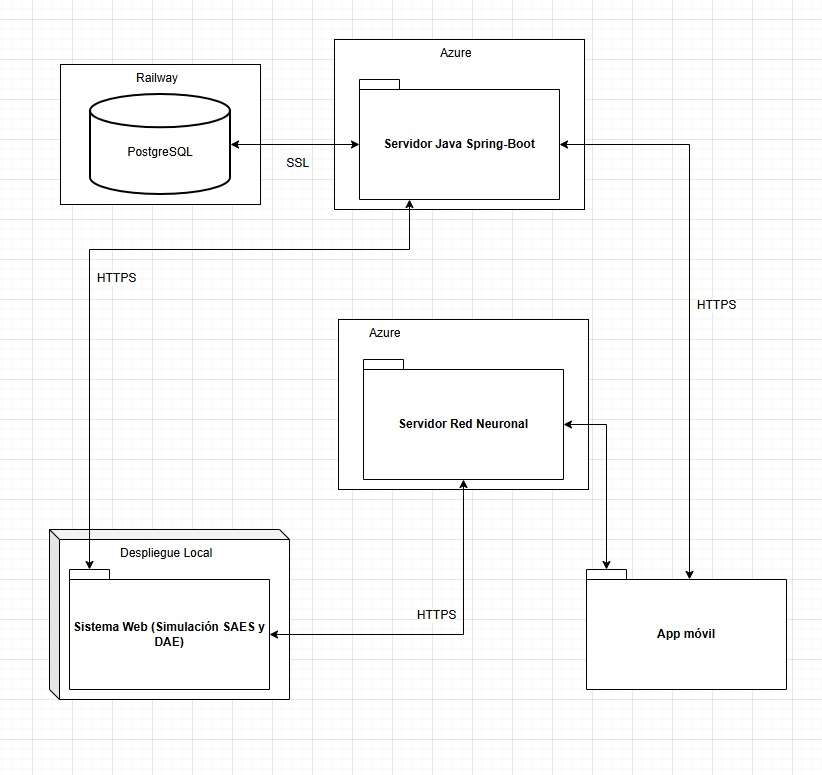
\includegraphics[width=0.8\textwidth]{images/DiagramaGeneralClases}
		\caption{Diagrama de la Estructura General del Sistema.}
		\label{fig:Diagrama de sistemas}
	\end{center}
\end{figure}

A continuación se entrara más en detalle en la estructura interna de los componentes del sistema del diagrama anterior.

\newpage

\section{Estructura Interna Detallada de la Aplicación Móvil} 

La Figura \ref{fig:Diagrama_app_movil_detallado} profundiza en la arquitectura interna de la aplicación móvil, presentando los paquetes y componentes clave que la conforman. 

El punto de entrada principal de la aplicación es la actividad `MainActivity.kt`, la cual orquesta el flujo general de la aplicación. 

La interfaz de usuario de la aplicación se construye dentro del paquete `Pantallas`. Este paquete contiene las implementaciones de las pantallas de la aplicación utilizando Jetpack Compose. Cada pantalla se define mediante funciones Composable, que describen la estructura y el comportamiento de la interfaz de usuario de manera declarativa. 

La lógica de presentación y la gestión del estado de las `Pantallas` se encuentran en el paquete llamado `com.example.prueba3.Views`. Dentro de este paquete, los ViewModels actúan como intermediarios, proporcionando los datos necesarios a las Composables y manejando la lógica de las interacciones del usuario. Existe una relación directa entre las `Pantallas` y los `Views`, donde cada pantalla suele estar asociada a un ViewModel específico. 

El modelo de datos de la aplicación se define principalmente en el paquete `com.example.prueba3.Clases`. Este paquete contiene las clases que representan los datos utilizados por la aplicación. En su mayoría, estas clases son Data Classes, diseñadas para almacenar y transportar datos de manera concisa y eficiente.

La comunicación con los servicios backend se gestiona a través del paquete `RetroFit`. Este paquete contiene las interfaces de Retrofit que definen los endpoints de la API de los servidores remotos. Estas interfaces especifican las operaciones HTTP (GET, POST y DELETE) necesarias para interactuar con el Servidor Java Spring-Boot y el Servidor Red Neuronal. Retrofit se encarga de generar el código necesario para realizar estas solicitudes y procesar las respuestas del servidor.

\newpage

\begin{figure}[htbp!]
	\begin{center}
		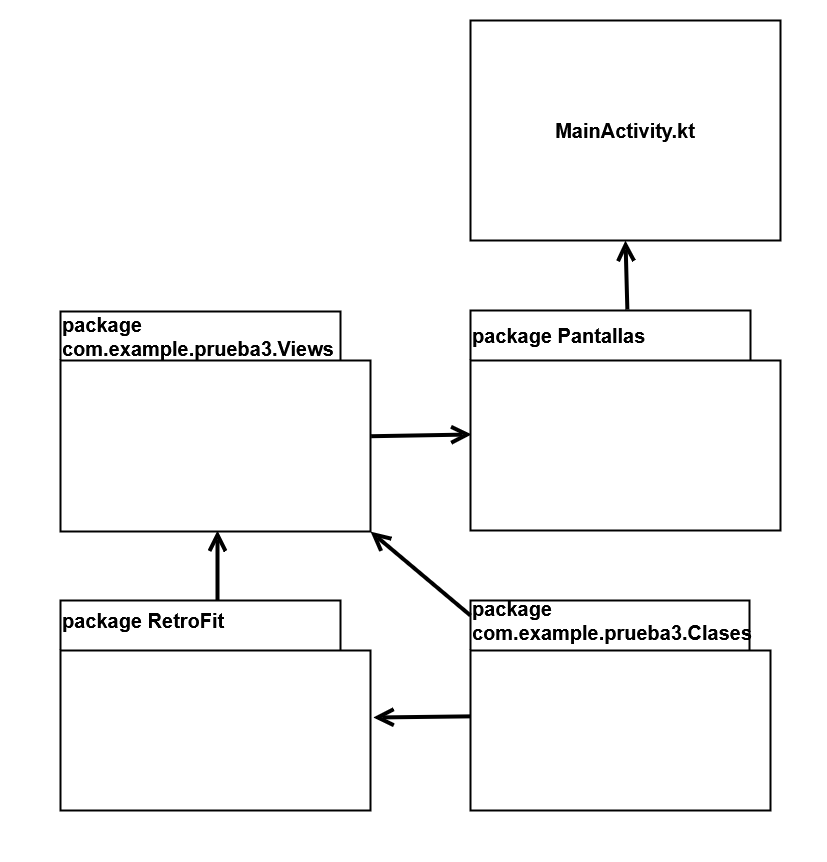
\includegraphics[width=0.6\textwidth]{DiagramasMoviles/DCM (1)}
		\caption{Estructura Interna Detallada de la Aplicación Móvil por Paquetes.}
		\label{fig:Diagrama_app_movil_detallado}
	\end{center}
\end{figure}



A continuación, se presentarán las clases contenidas en los paquetes `com.example.prueba3.Views` (ViewModels), `com.example.prueba3.Clases` (Data Classes) y las interfaces definidas en el paquete `RetroFit`, detallando su estructura y funcionalidad sección por sección. Adicionalmente, se incluirán diagramas de componentes específicos para cada una de las `Pantallas` de la aplicación móvil, ilustrando la composición de sus elementos y sus dependencias internas.

\newpage

\subsection{Diagramas de Componentes de Pantallas}

Para una comprensión más profunda de la arquitectura de la interfaz de usuario de la aplicación móvil, a continuación se presentan los diagramas de componentes para cada una de las pantallas principales. Estos diagramas ilustran la composición interna de cada pantalla, mostrando los elementos de la interfaz de usuario (Composables), los datos que manejan y las posibles interacciones o dependencias con otros componentes. Cada diagrama proporciona una vista modular de la pantalla, facilitando la visualización de cómo se construyen las distintas secciones de la interfaz de usuario y cómo se relacionan entre sí. La Figura \ref{fig:Pantallas} muestra las pantallas (archivos .kt) presentes en package.Pantallas.

\begin{figure}[htbp!]
	\begin{center}
		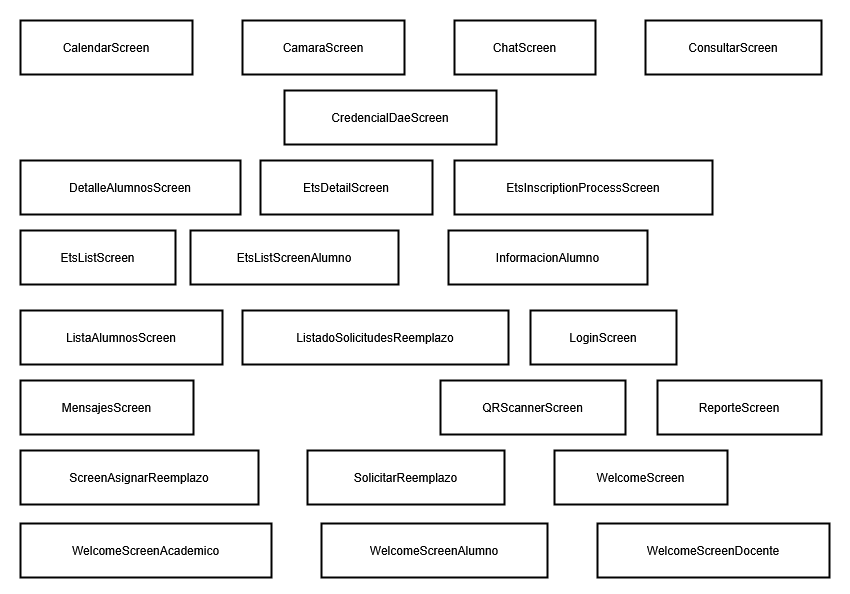
\includegraphics[width=0.9\textwidth]{DiagramasMoviles/DCM (12)}
		\caption{Pantallas presentes en package.Pantallas (archivos .kt).}
		\label{fig:Pantallas}
	\end{center}
\end{figure}


\newpage

\subsection{Diagrama de Componentes de CalendarScreen.kt}

La Figura \ref{fig:Componentes_1} muestra el diagrama de componentes para CalendarScreen.kt que es un composable que contiene a la \IUref{IU02}{Pantalla Consultar calendario escolar}, que muestra el calendario escolar y permite al usuario ver cuantos días faltan para el periodo de ETS próximo si esta disponible.

\begin{figure}[htbp!]
	\begin{center}
		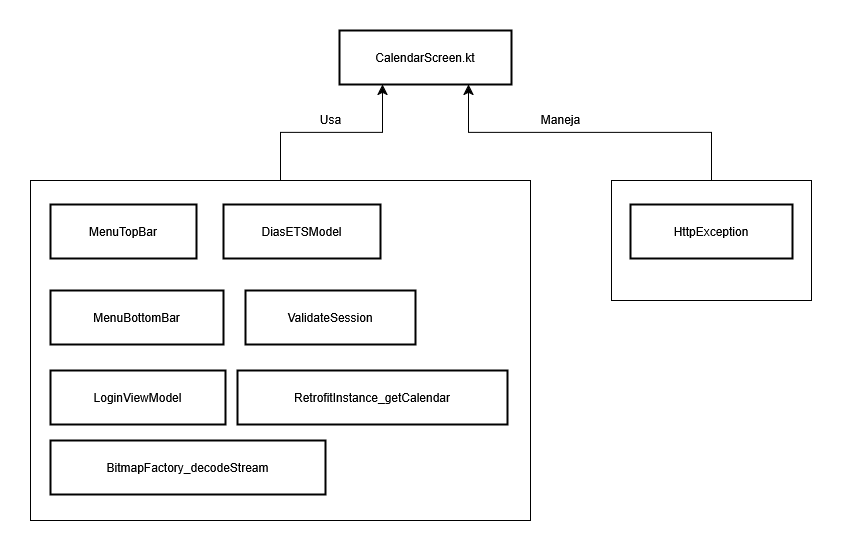
\includegraphics[width=0.9\textwidth]{DiagramasMoviles/DCM (13)}
		\caption{Diagrama de componentes para CalendarScreen.kt .}
		\label{fig:Componentes_1}
	\end{center}
\end{figure}

\newpage

\subsection{Diagrama de Componentes de CamaraScreen.kt}

La Figura \ref{fig:Componentes_2} muestra el diagrama de componentes para CamaraScreen.kt que es un composable que contiene a la \IUref{IU17}{Pantalla de Reconocimiento facial} y la \IUref{IU19}{Pantalla de Reconocimiento facial alumno}, que muestran la cámara usada para obtener la foto que se usara para el proceso de reconocimiento facial.

\begin{figure}[htbp!]
	\begin{center}
		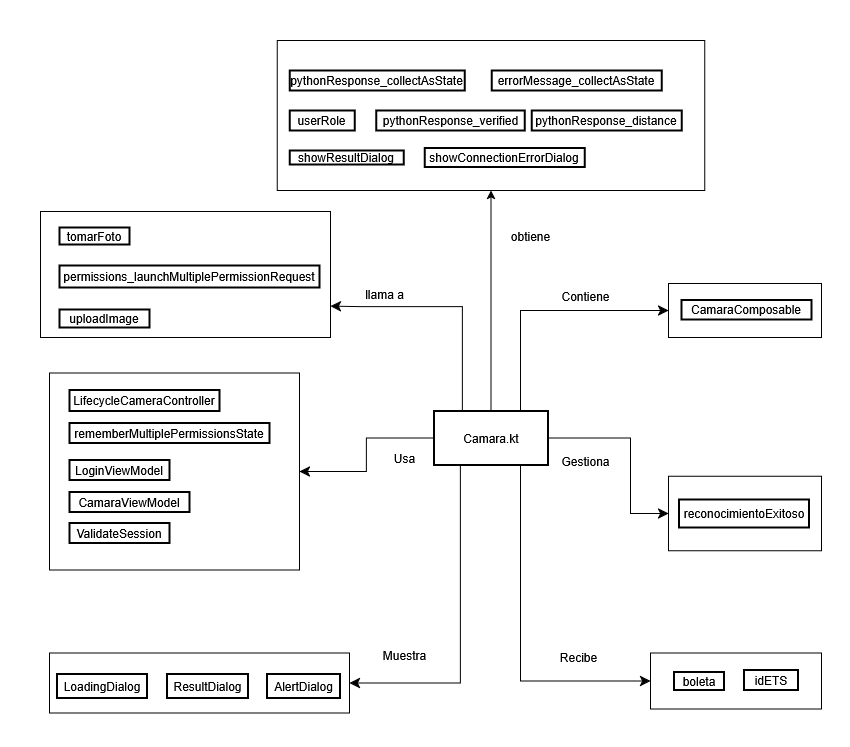
\includegraphics[width=0.9\textwidth]{DiagramasMoviles/DCM (14)}
		\caption{Diagrama de componentes para CamaraScreen.kt .}
		\label{fig:Componentes_2}
	\end{center}
\end{figure}

\newpage

\subsection{Diagrama de Componentes de ChatScreen.kt}

La Figura \ref{fig:Componentes_3} muestra el diagrama de componentes para ChatScreen.kt que es un composable que contiene una pantalla que muestra el chat de mensajes que pueden usar los usuarios.

\begin{figure}[htbp!]
	\begin{center}
		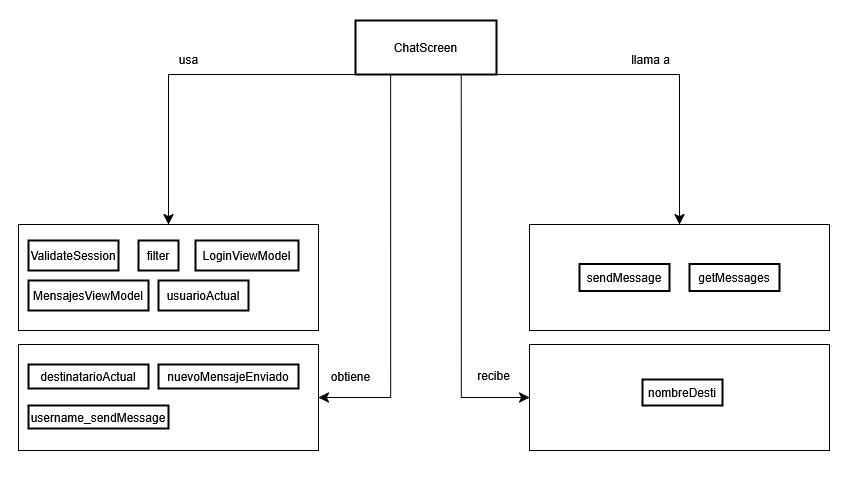
\includegraphics[width=0.9\textwidth]{DiagramasMoviles/DCM (15)}
		\caption{Diagrama de componentes para ChatScreen.kt .}
		\label{fig:Componentes_3}
	\end{center}
\end{figure}

\newpage

\subsection{Diagrama de Componentes de ConsultarScreen.kt}

La Figura \ref{fig:Componentes_4} muestra el diagrama de componentes para ConsultarScreen.kt que es un composable que contiene a la \IUref{IU12}{Pantalla Buscar alumno}, que muestra la lista de los alumnos inscritos a un ETS para el personal de seguridad y le permite filtrarlos por nombre o boleta.

\begin{figure}[htbp!]
	\begin{center}
		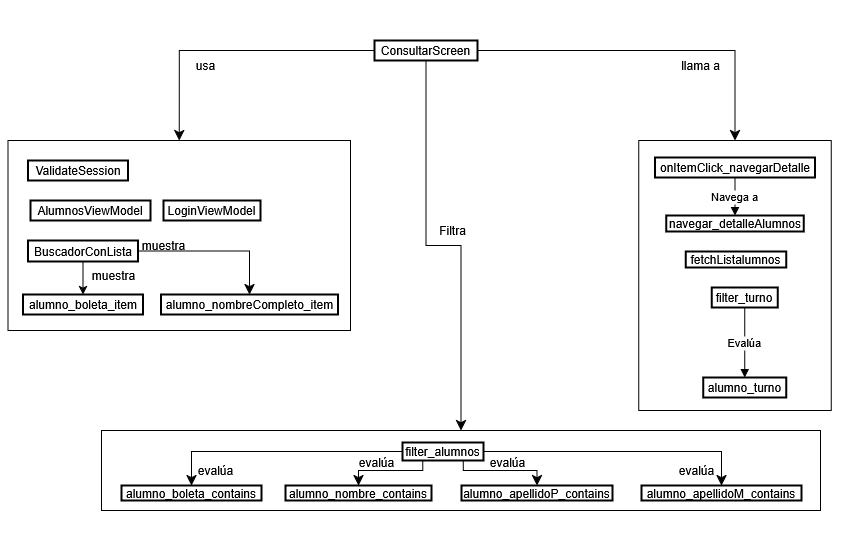
\includegraphics[width=0.9\textwidth]{DiagramasMoviles/DCM (16)}
		\caption{Diagrama de componentes para ConsultarScreen.kt .}
		\label{fig:Componentes_4}
	\end{center}
\end{figure}

\newpage

\subsection{Diagrama de Componentes de CredencialDaeScreen.kt}

La Figura \ref{fig:Componentes_5} muestra el diagrama de componentes para CredencialDaeScreen.kt que es un composable que contiene a la \IUref{IU11}{Pantalla Credencial del alumno}, que muestra la comparación de la credencial de la DAE con la credencial creada por el sistema.

\begin{figure}[htbp!]
	\begin{center}
		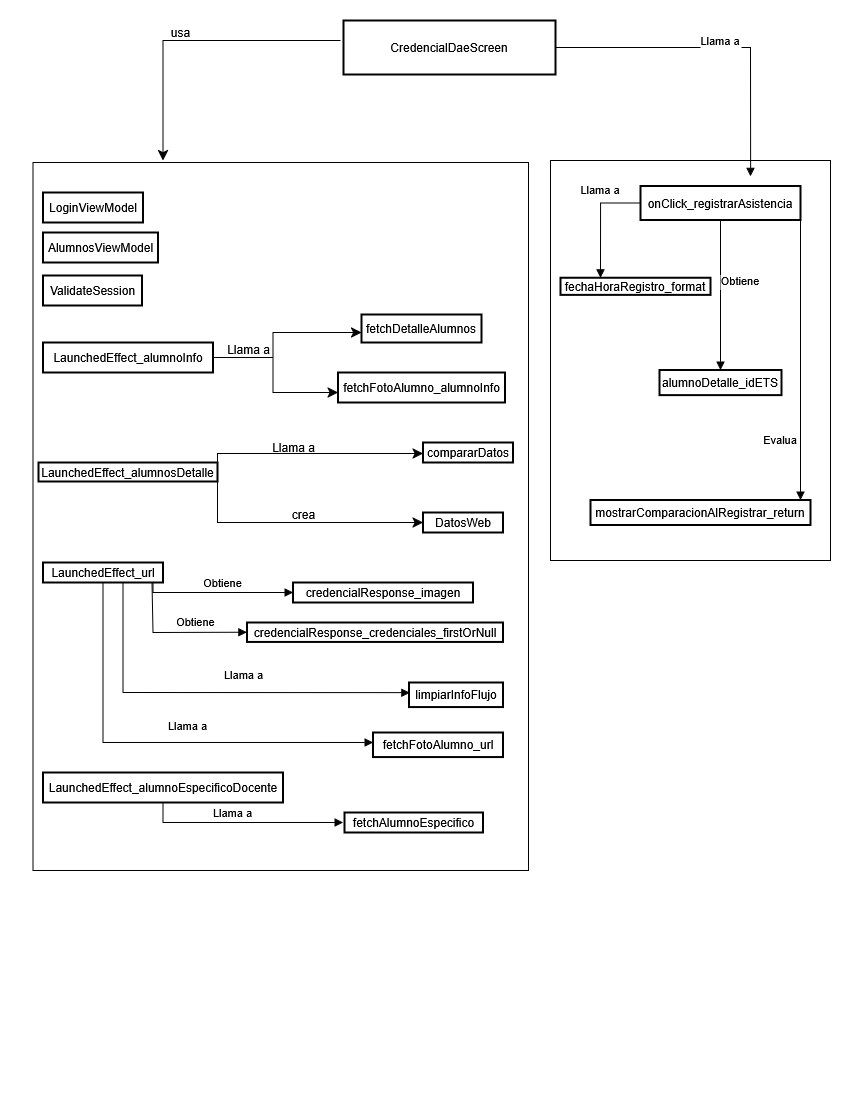
\includegraphics[width=0.9\textwidth]{DiagramasMoviles/DCM (17)}
		\caption{Diagrama de componentes para CredencialDaeScreen.kt .}
		\label{fig:Componentes_5}
	\end{center}
\end{figure}

\newpage

\subsection{Diagrama de Componentes de DetallesAlumnosScreen.kt}

La Figura \ref{fig:Componentes_6} muestra el diagrama de componentes para DetallesAlumnosScreen.kt que es un composable que contiene a la \IUref{IU11}{Pantalla Credencial del alumno}, que en este caso muestra la información relevante del alumno.

\begin{figure}[htbp!]
	\begin{center}
		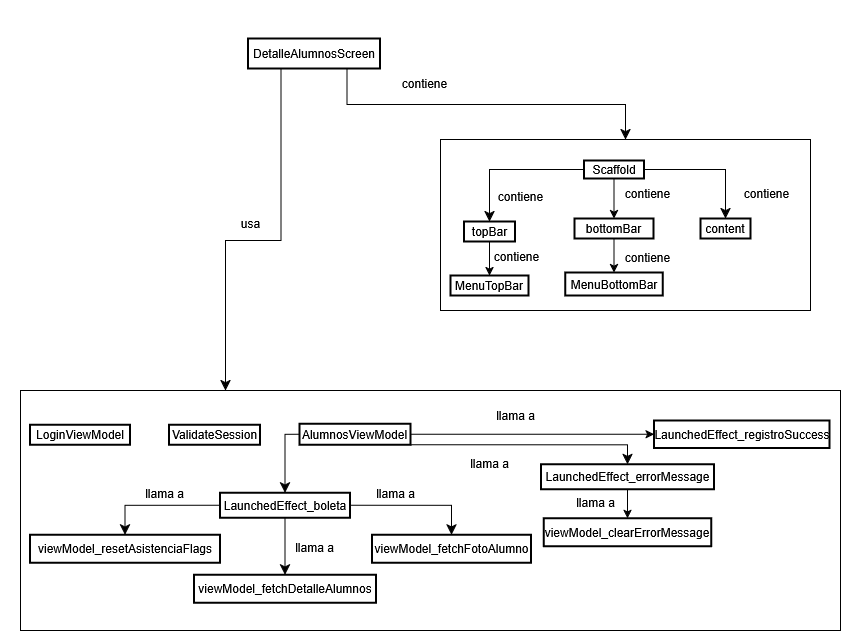
\includegraphics[width=0.9\textwidth]{DiagramasMoviles/DCM (19)}
		\caption{Diagrama de componentes para DetallesAlumnosScreen.kt .}
		\label{fig:Componentes_6}
	\end{center}
\end{figure}

\newpage

\subsection{Diagrama de Componentes de EtsDetailScreen.kt}

La Figura \ref{fig:Componentes_7} muestra el diagrama de componentes para EtsDetailScreen.kt que es un composable que contiene a la \IUref{IU06}{Pantalla Información de ETS} y \IUref{IU16}{Pantalla Información de ETS del alumno}, que muestra la información del ETS elegido por el usuario.

\begin{figure}[htbp!]
	\begin{center}
		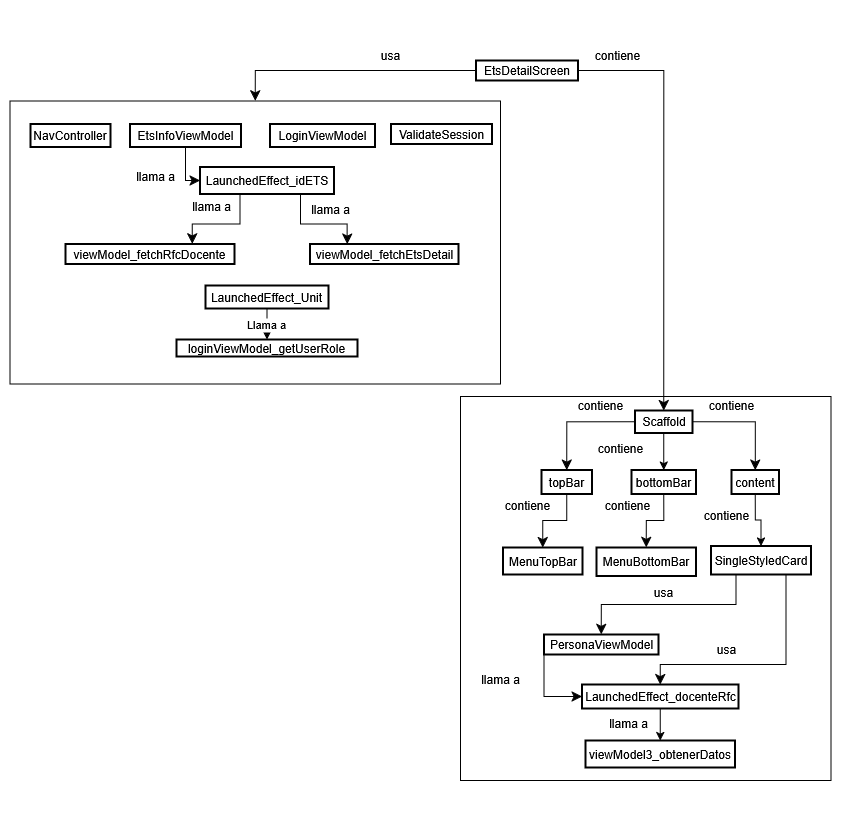
\includegraphics[width=0.9\textwidth]{DiagramasMoviles/DCM (20)}
		\caption{Diagrama de componentes para EtsDetailScreen.kt .}
		\label{fig:Componentes_7}
	\end{center}
\end{figure}

\newpage

\subsection{Diagrama de Componentes de EtsInscriptionProcessScreen.kt}

La Figura \ref{fig:Componentes_8} muestra el diagrama de componentes para ETSInscriptionProcessScreen.kt que es un composable que contiene a la \IUref{IU18}{Pantalla de Detalles del proceso de ETS}, que muestra la información necesaria para inscribirse a un ETS.

\begin{figure}[htbp!]
	\begin{center}
		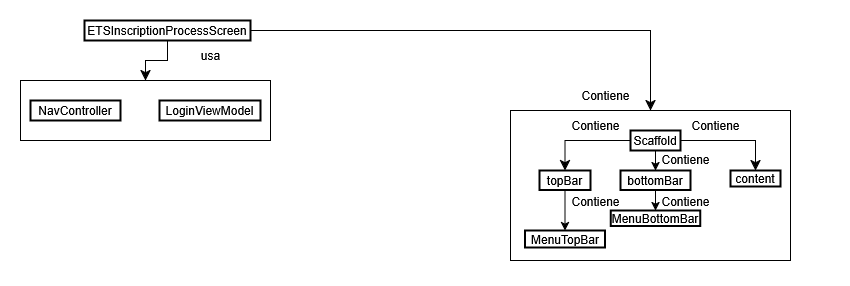
\includegraphics[width=0.9\textwidth]{DiagramasMoviles/DCM (21)}
		\caption{Diagrama de componentes para ETSInscriptionProcessScreen.kt .}
		\label{fig:Componentes_8}
	\end{center}
\end{figure}

\newpage

\subsection{Diagrama de Componentes de EtsListScreen.kt}

La Figura \ref{fig:Componentes_9} muestra el diagrama de componentes para EtsListScreen.kt que es un composable que contiene a la \IUref{IU05}{Pantalla Consultar ETS}, que muestra la lista de ETS del docente.

\begin{figure}[htbp!]
	\begin{center}
		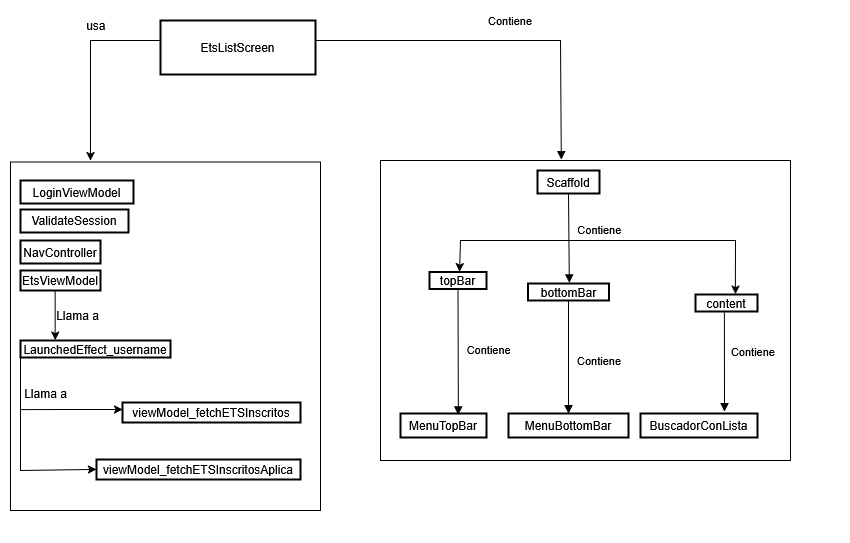
\includegraphics[width=0.9\textwidth]{DiagramasMoviles/DCM (22)}
		\caption{Diagrama de componentes para EtsListScreen.kt .}
		\label{fig:Componentes_9}
	\end{center}
\end{figure}

\newpage

\subsection{Diagrama de Componentes de EtsListScreenAlumno.kt}

La Figura \ref{fig:Componentes_10} muestra el diagrama de componentes para EtsListScreenAlumno.kt que es un composable que contiene a la \IUref{IU05}{Pantalla Consultar ETS}, que muestra la lista de ETS del alumno.

\begin{figure}[htbp!]
	\begin{center}
		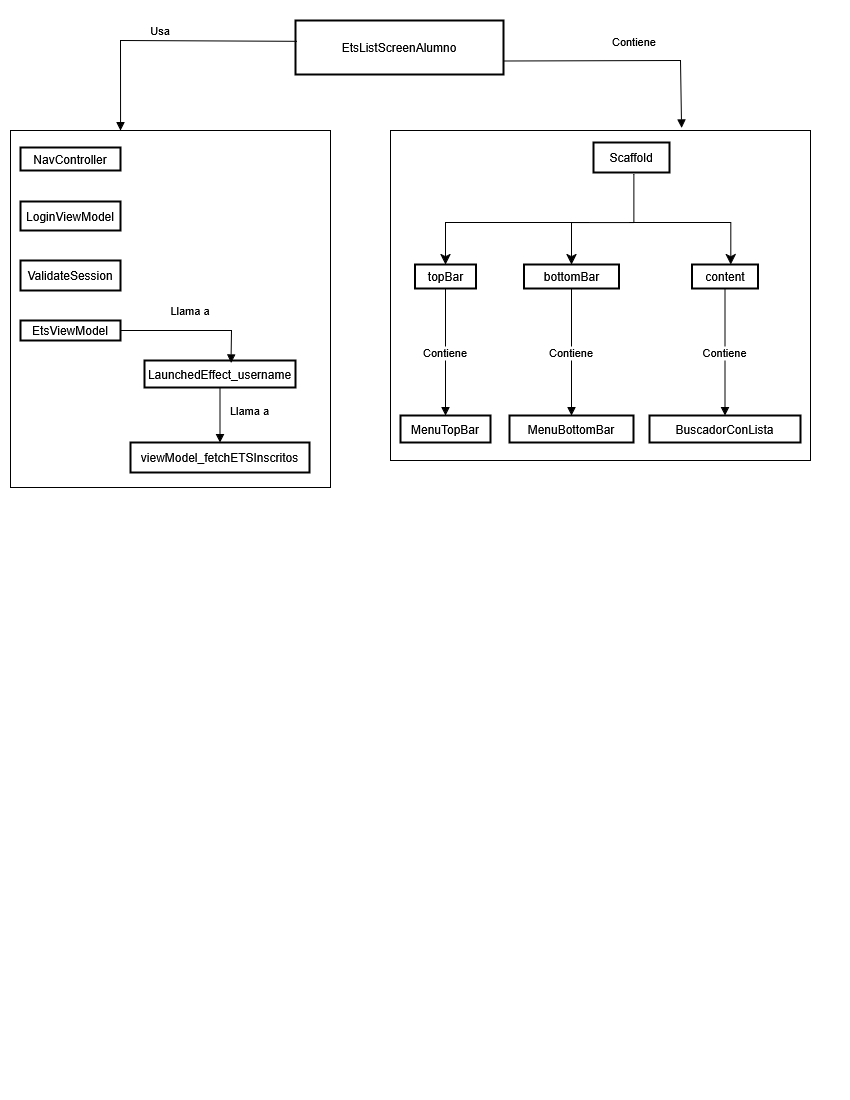
\includegraphics[width=0.9\textwidth]{DiagramasMoviles/DCM (23)}
		\caption{Diagrama de componentes para EtsListScreenAlumno.kt .}
		\label{fig:Componentes_10}
	\end{center}
\end{figure}

\newpage

\subsection{Diagrama de Componentes de InformacionAlumno.kt}

La Figura \ref{fig:Componentes_11} muestra el diagrama de componentes para InformacionAlumno.kt que es un composable que contiene a la \IUref{IUE07}{Creación del reporte}, que se utiliza para la creación de reportes y a su vez muestra la información esencial del alumno seleccionado.

\begin{figure}[htbp!]
	\begin{center}
		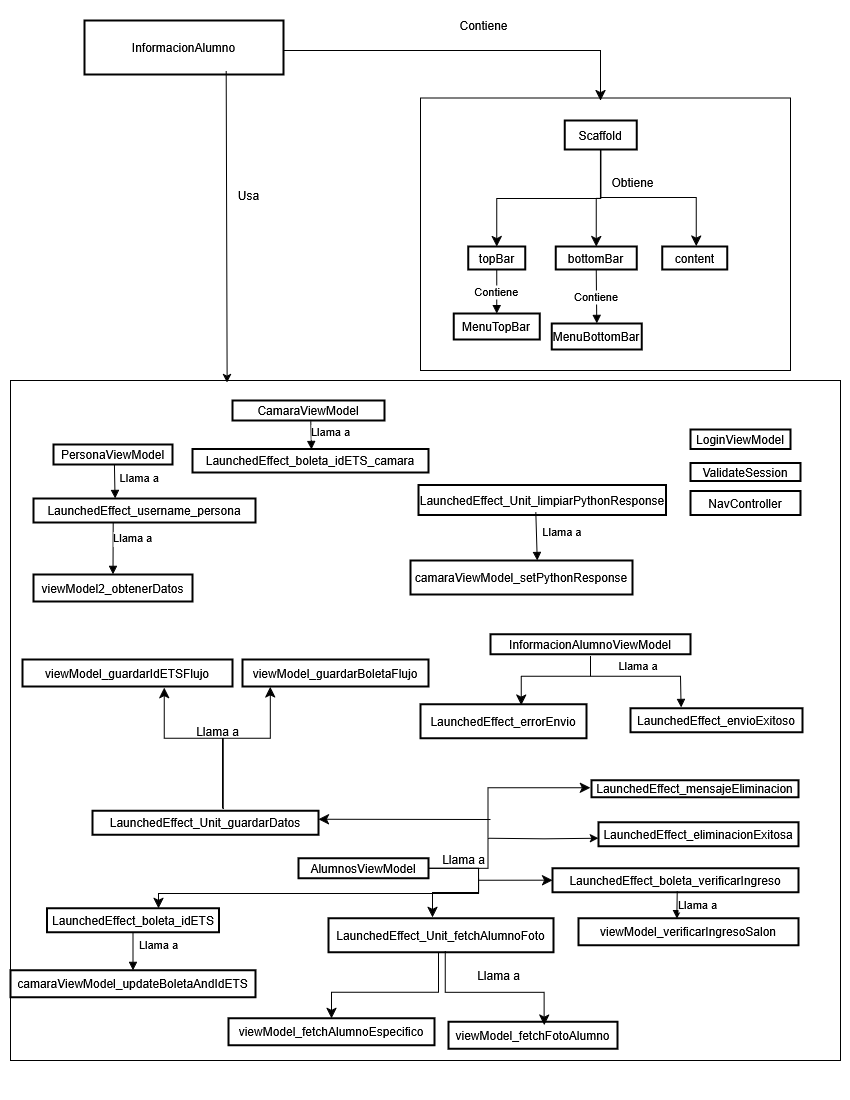
\includegraphics[width=0.7\textwidth]{DiagramasMoviles/DCM (24)}
		\caption{Diagrama de componentes para InformacionAlumno.kt .}
		\label{fig:Componentes_11}
	\end{center}
\end{figure}

\newpage

\subsection{Diagrama de Componentes de ListaAlumnosScreen.kt}

La Figura \ref{fig:Componentes_12} muestra el diagrama de componentes para ListaAlumnosScreen.kt que es un composable que contiene a la \IUref{IU08}{Pantalla Lista de asistencia de ETS}, que es la que le muestra la lista de alumnos inscritos a un ETS al docente, junto con su estado de asistencia con un icono.

\begin{figure}[htbp!]
	\begin{center}
		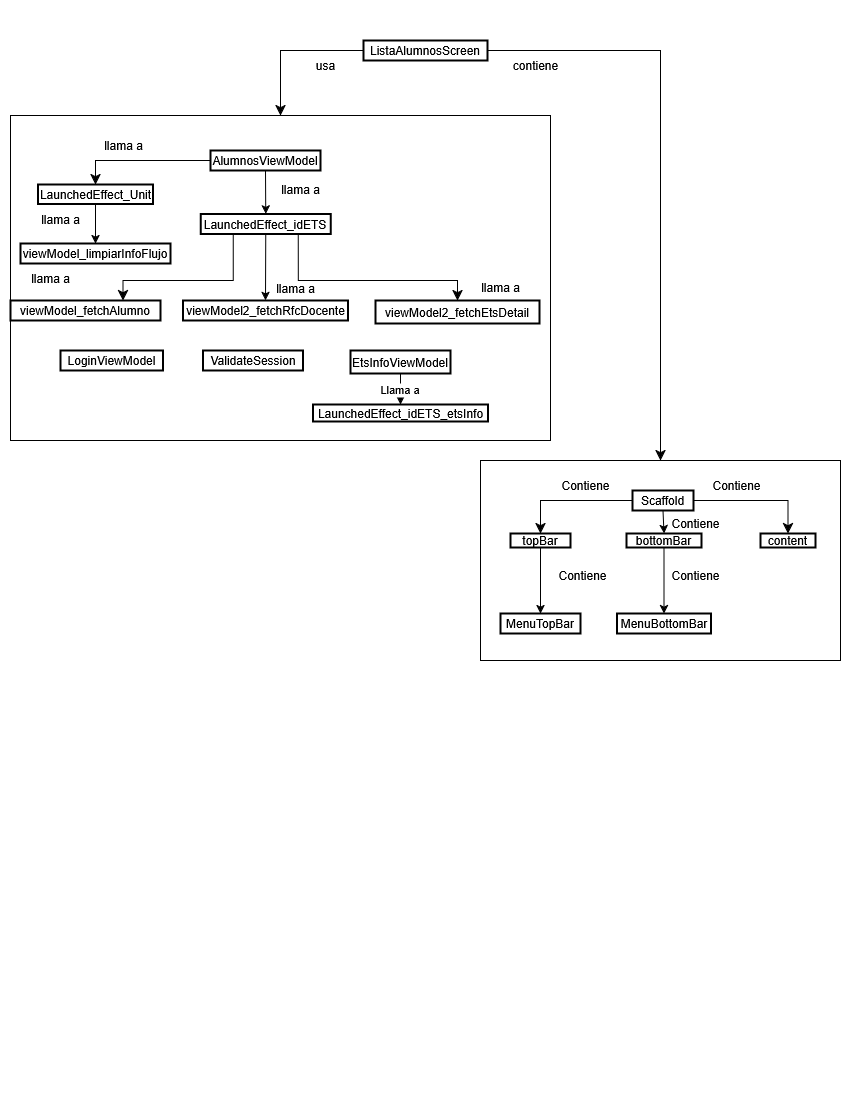
\includegraphics[width=0.9\textwidth]{DiagramasMoviles/DCM (25)}
		\caption{Diagrama de componentes para ListaAlumnosScreen.kt .}
		\label{fig:Componentes_12}
	\end{center}
\end{figure}

\newpage

\subsection{Diagrama de Componentes de ListadoSolicitudesReemplazo.kt}

La Figura \ref{fig:Componentes_13} muestra el diagrama de componentes para ListadoSolicitudesReemplazo.kt que es un composable que contiene una pantalla dedica a la visualización de las solicitudes de reemplazo y sus estados de aceptación o denegación. 

\begin{figure}[htbp!]
	\begin{center}
		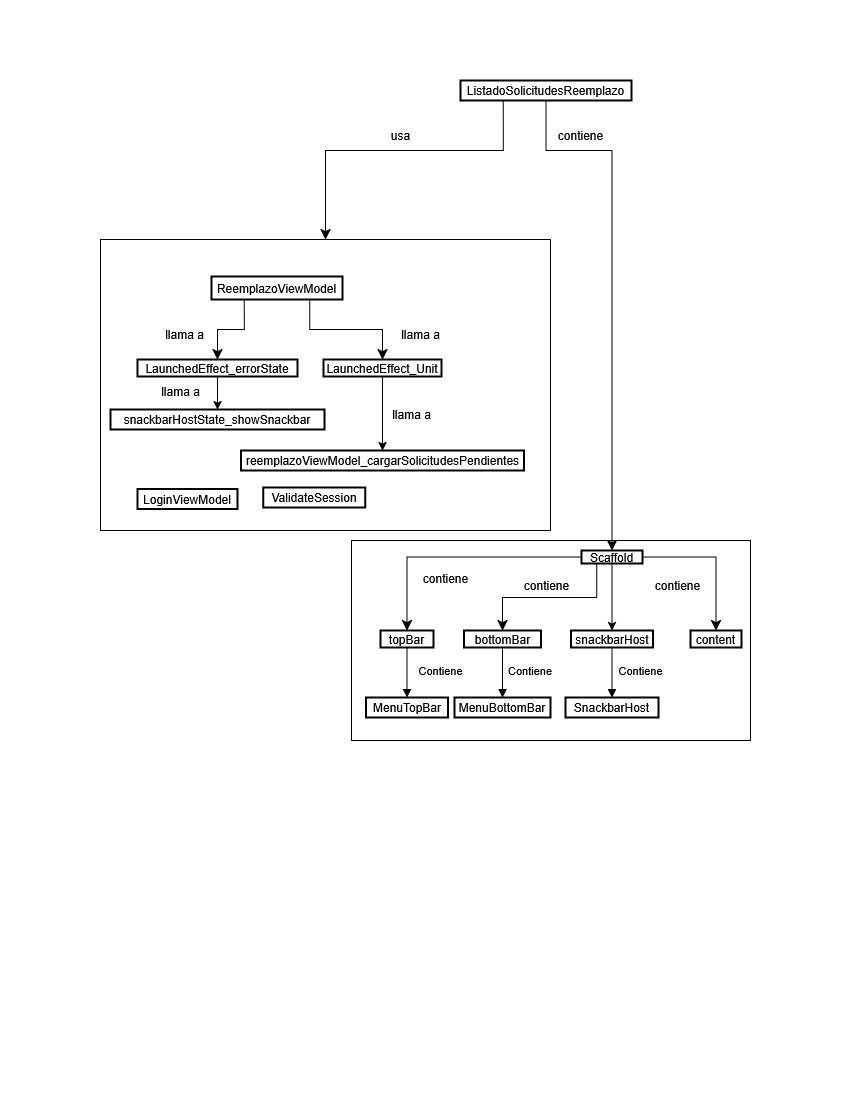
\includegraphics[width=0.9\textwidth]{DiagramasMoviles/DCM (26)}
		\caption{Diagrama de componentes para ListadoSolicitudesReemplazo.kt .}
		\label{fig:Componentes_13}
	\end{center}
\end{figure}

\newpage

\subsection{Diagrama de Componentes de LoginScreen.kt}

La Figura \ref{fig:Componentes_14} muestra el diagrama de componentes para LoginScreen.kt que es un composable que contiene a la \IUref{IU01}{Pantalla Iniciar sesión del sistema móvil}, que es el login de la aplicación móvil.

\begin{figure}[htbp!]
	\begin{center}
		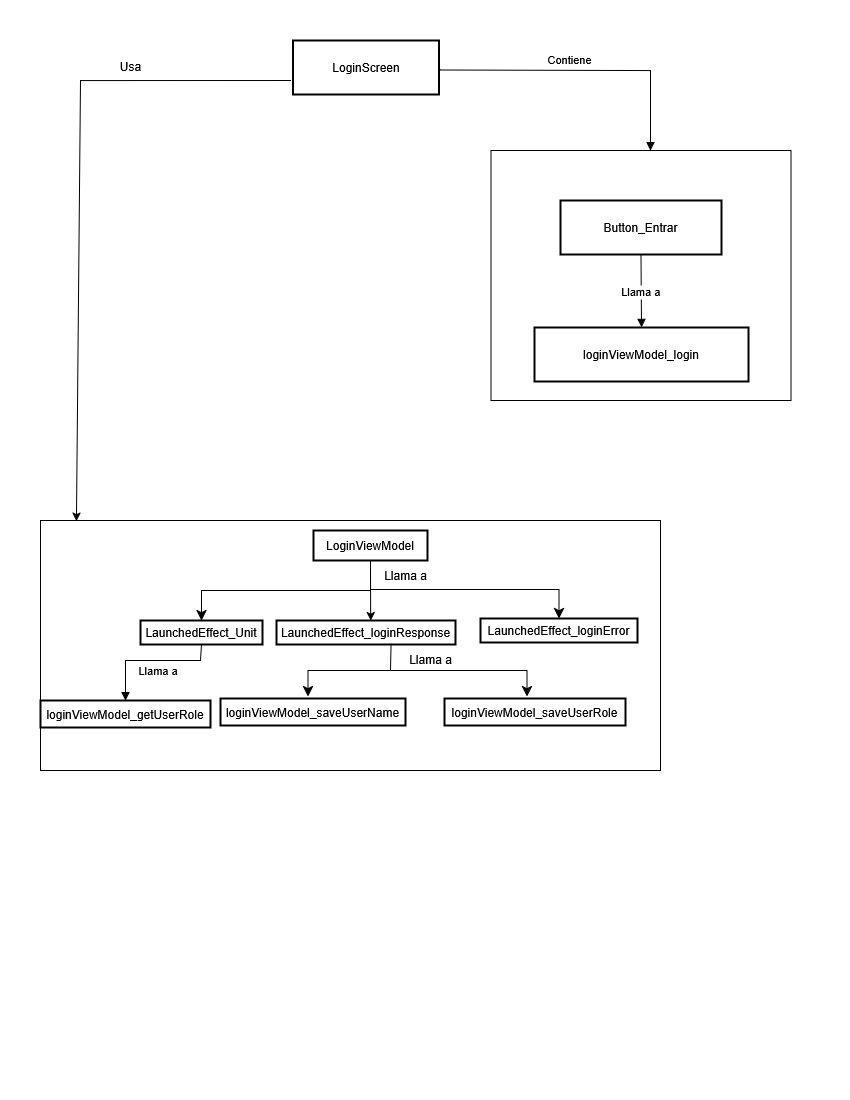
\includegraphics[width=0.9\textwidth]{DiagramasMoviles/DCM (27)}
		\caption{Diagrama de componentes para LoginScreen.kt .}
		\label{fig:Componentes_14}
	\end{center}
\end{figure}

\newpage

\subsection{Diagrama de Componentes de MensajesScreen.kt}

La Figura \ref{fig:Componentes_15} muestra el diagrama de componentes para MensajesScreen.kt que es un composable que es la pantalla donde se ven los mensaje específicos mandados a otro usuario.

\begin{figure}[htbp!]
	\begin{center}
		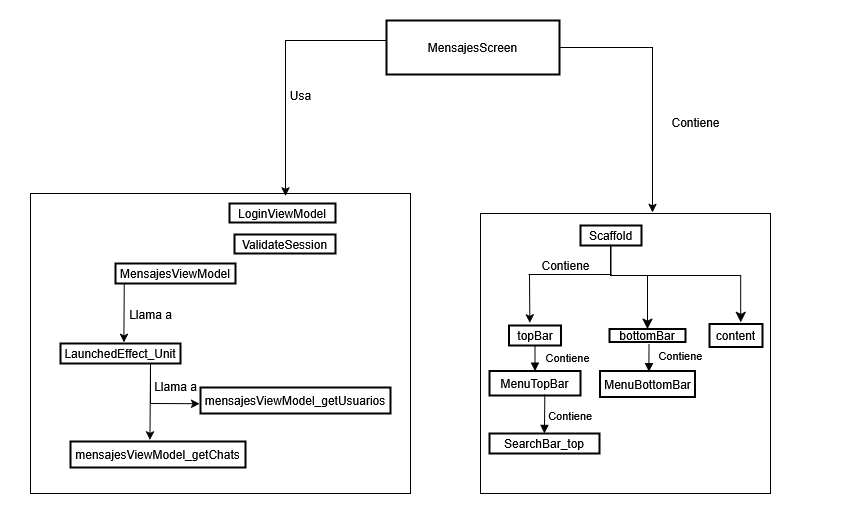
\includegraphics[width=0.9\textwidth]{DiagramasMoviles/DCM (28)}
		\caption{Diagrama de componentes para MensajesScreen.kt .}
		\label{fig:Componentes_15}
	\end{center}
\end{figure}

\newpage

\subsection{Diagrama de Componentes de QRScannerScreen.kt}

La Figura \ref{fig:Componentes_16} muestra el diagrama de componentes para QRScannerScreen.kt que es un composable que contiene a la \IUref{IU10}{Pantalla Código QR}, que muestra la cámara para poder escanear el código QR de la credencial del alumno.

\begin{figure}[htbp!]
	\begin{center}
		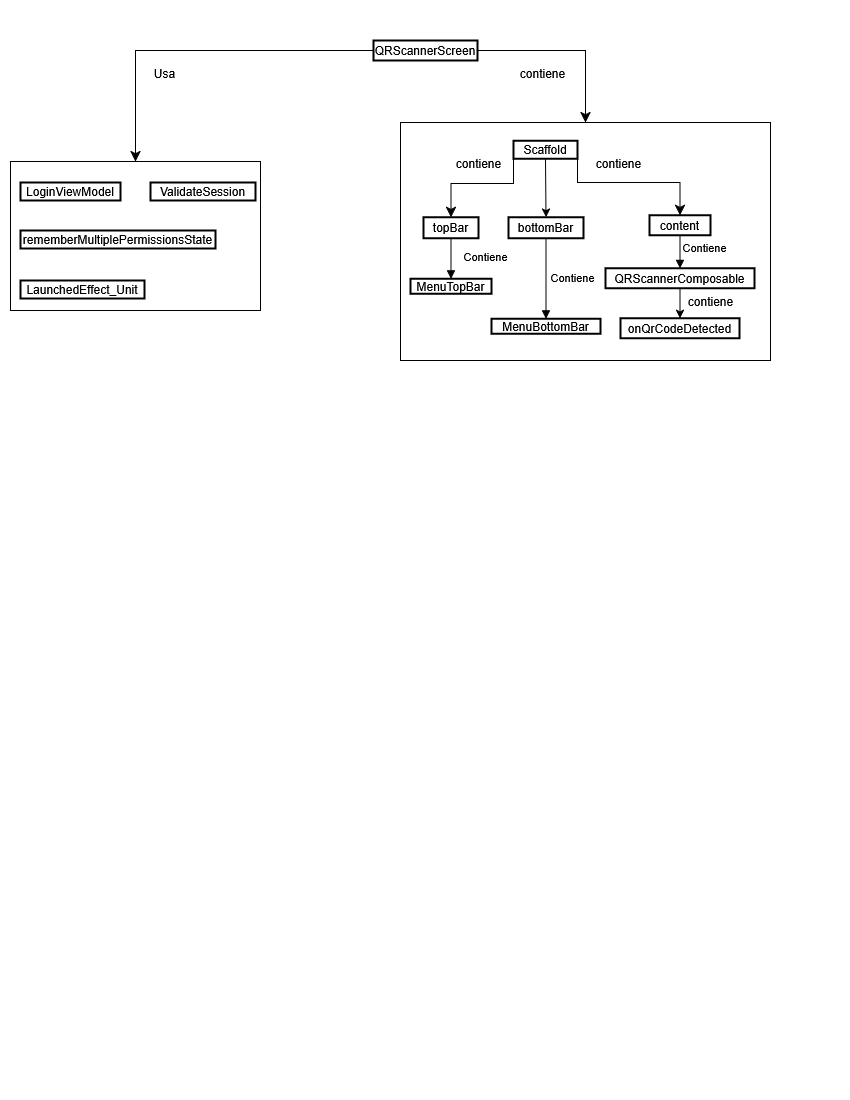
\includegraphics[width=0.9\textwidth]{DiagramasMoviles/DCM (29)}
		\caption{Diagrama de componentes para QRScannerScreen.kt .}
		\label{fig:Componentes_16}
	\end{center}
\end{figure}

\newpage

\subsection{Diagrama de Componentes de ReporteScreen.kt}

La Figura \ref{fig:Componentes_17} muestra el diagrama de componentes para ReporteScreen.kt que es un composable que contiene a la \IUref{IU20}{Pantalla Reporte del Alumno}, que es donde el docente puede revisar el reporte de la asistencia del alumno.

\begin{figure}[htbp!]
	\begin{center}
		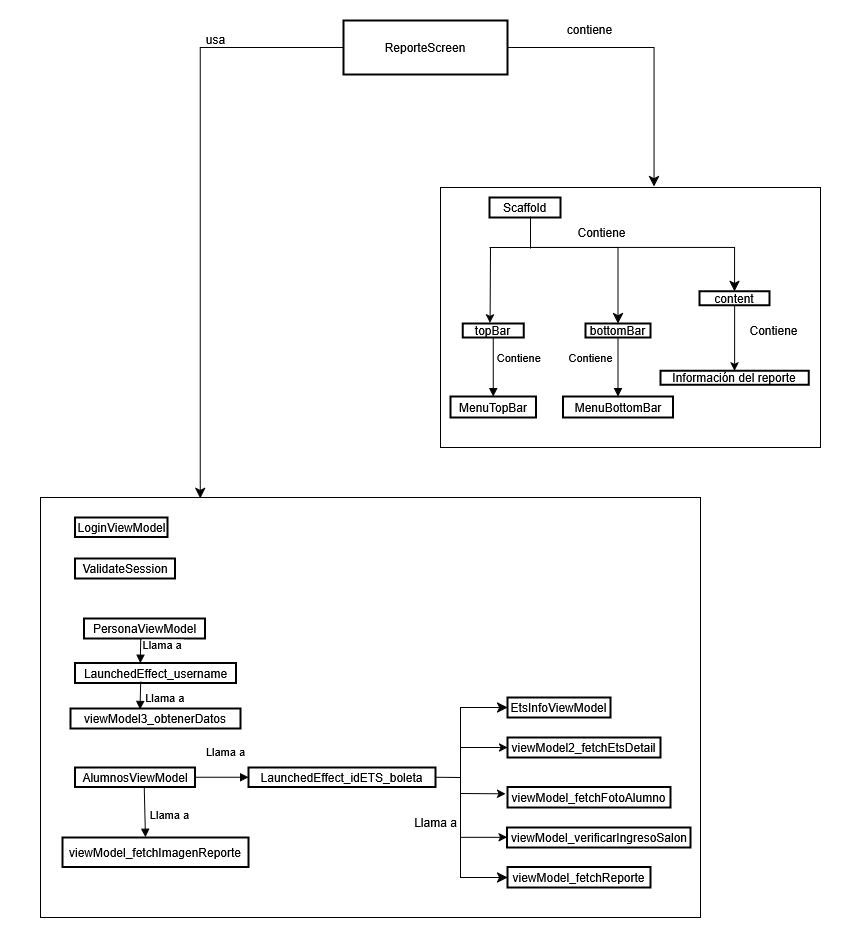
\includegraphics[width=0.7\textwidth]{DiagramasMoviles/DCM (30)}
		\caption{Diagrama de componentes para ReporteScreen.kt .}
		\label{fig:Componentes_17}
	\end{center}
\end{figure}

\newpage

\subsection{Diagrama de Componentes de ScreenAsignarremplazo.kt}

La Figura \ref{fig:Componentes_18} muestra el diagrama de componentes para ScreenAsignarremplazo.kt que es un composable que contiene a la pantalla \IUref{IU09}{Asignar docente de remplazo}, que es donde el jefe de departamento y/o el presidente de academia pueden responder a las solicitudes de reemplazo.

\begin{figure}[htbp!]
	\begin{center}
		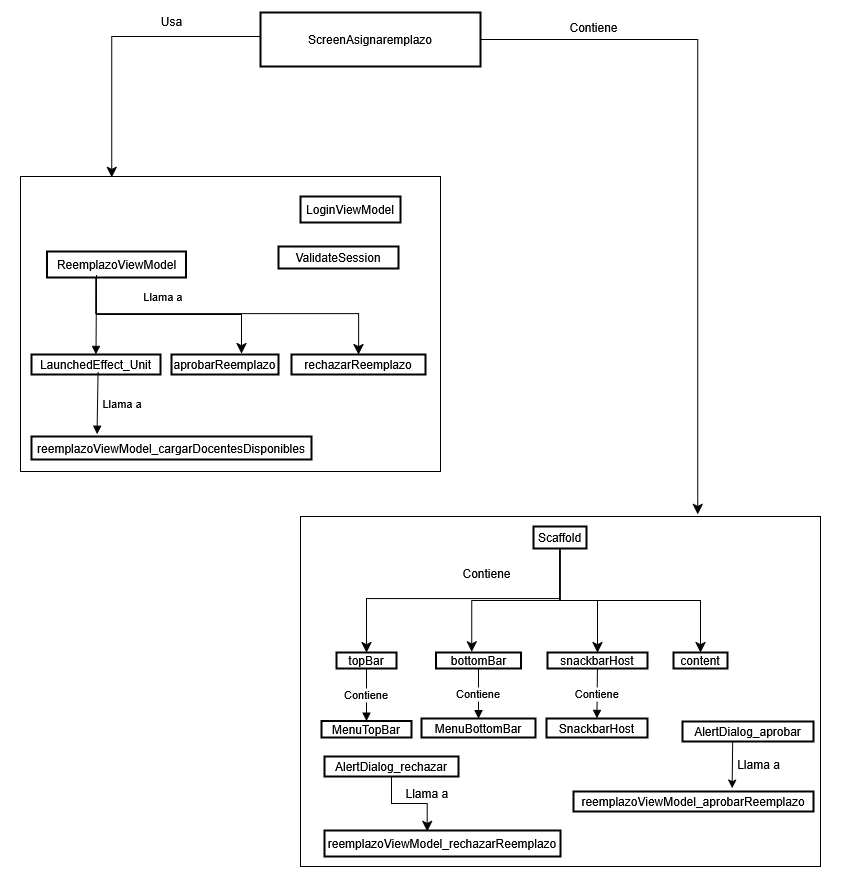
\includegraphics[width=0.9\textwidth]{DiagramasMoviles/DCM (31)}
		\caption{Diagrama de componentes para ScreenAsignarremplazo.kt .}
		\label{fig:Componentes_18}
	\end{center}
\end{figure}

\newpage

\subsection{Diagrama de Componentes de SolicitarReemplazo.kt}

La Figura \ref{fig:Componentes_19} muestra el diagrama de componentes para SolicitarReemplazo.kt que es un composable que contiene a la \IUref{IU07}{Pantalla de Solicitar remplazo}, que es donde el docente puede pedir un reemplazo como aplacador del ETS.

\begin{figure}[htbp!]
	\begin{center}
		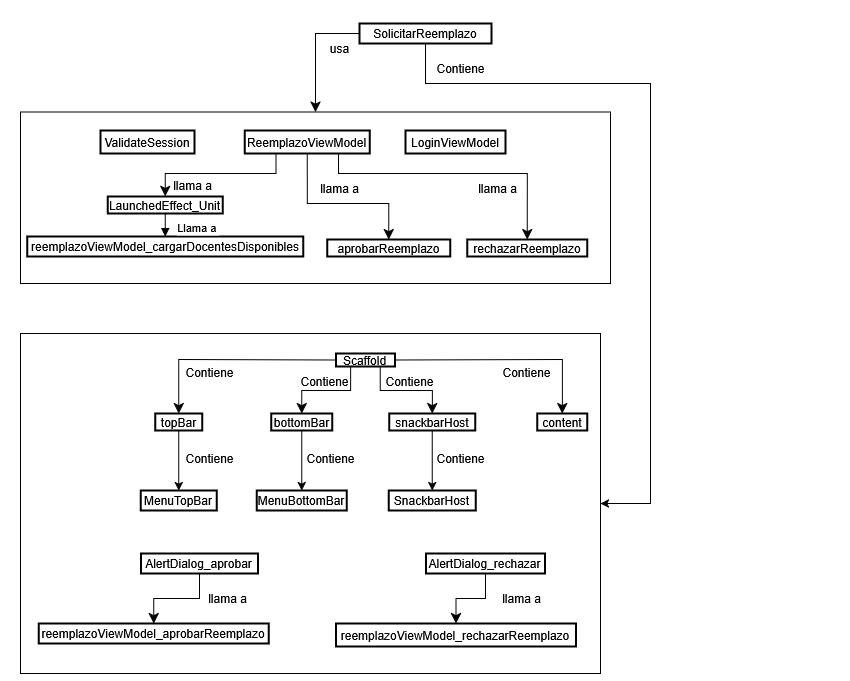
\includegraphics[width=0.9\textwidth]{DiagramasMoviles/DCM (32)}
		\caption{Diagrama de componentes para SolicitarReemplazo.kt .}
		\label{fig:Componentes_19}
	\end{center}
\end{figure}

\newpage

\subsection{Diagrama de Componentes de WelcomeScreen.kt}

La Figura \ref{fig:Componentes_20} muestra el diagrama de componentes para WelcomeScreen.kt que es un composable que contiene a la \IUref{IUE02}{Pantalla de saludo del personal de seguridad}, que es la pantalla de inicio del personal de seguridad (donde pude seleccionar la operación que quiere realizar y ver un saludo con su nombre).

\begin{figure}[htbp!]
	\begin{center}
		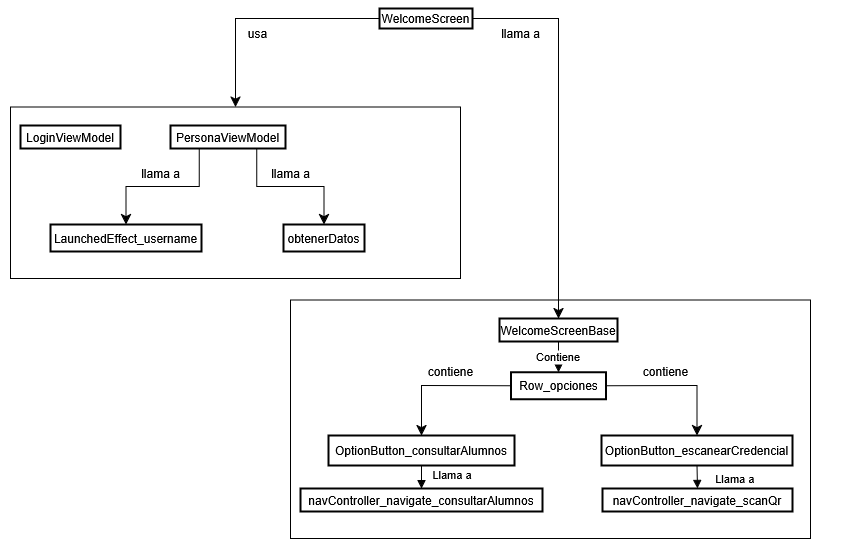
\includegraphics[width=0.9\textwidth]{DiagramasMoviles/DCM (33)}
		\caption{Diagrama de componentes para WelcomeScreen.kt .}
		\label{fig:Componentes_20}
	\end{center}
\end{figure}

\newpage

\subsection{Diagrama de Componentes de WelcomeScreenAcademico.kt}

La Figura \ref{fig:Componentes_21} muestra el diagrama de componentes para WelcomeScreenAcademico.kt que es un composable que contiene a la pantalla \IUref{IUE06}{saludo del presidente de academia y el jefe de departamento}, que es la pantalla de inicio del jefe de departamento y/o el presidente de academia (donde pude seleccionar la operación que quiere realizar y ver un saludo con su nombre).

\begin{figure}[htbp!]
	\begin{center}
		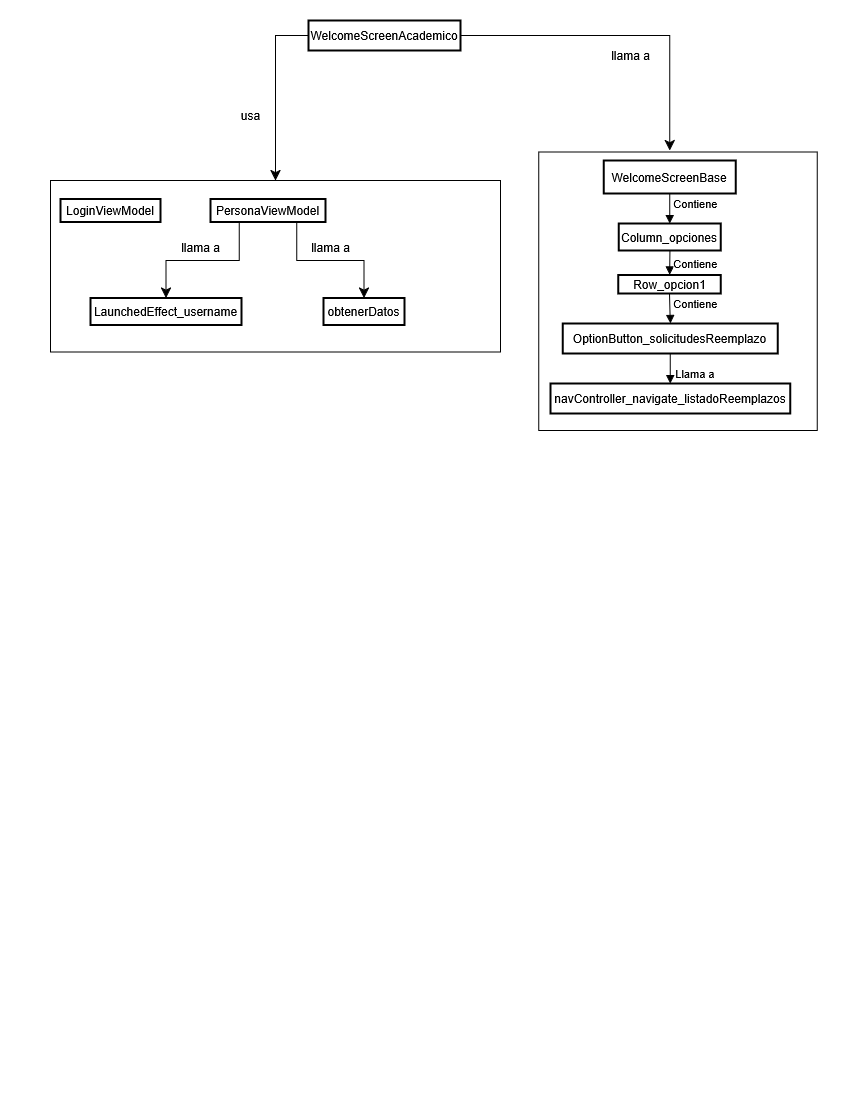
\includegraphics[width=0.9\textwidth]{DiagramasMoviles/DCM (34)}
		\caption{Diagrama de componentes para WelcomeScreenAcademico.kt .}
		\label{fig:Componentes_21}
	\end{center}
\end{figure}

\newpage

\subsection{Diagrama de Componentes de WelcomeScreenAlumno.kt}

La Figura \ref{fig:Componentes_22} muestra el diagrama de componentes para WelcomeScreenAlumno.kt que es un composable que contiene a la pantalla \IUref{IUE03}{Pantalla saludo del alumno}, que es la pantalla de inicio del Alumno (donde pude seleccionar la operación que quiere realizar y ver un saludo con su nombre).

\begin{figure}[htbp!]
	\begin{center}
		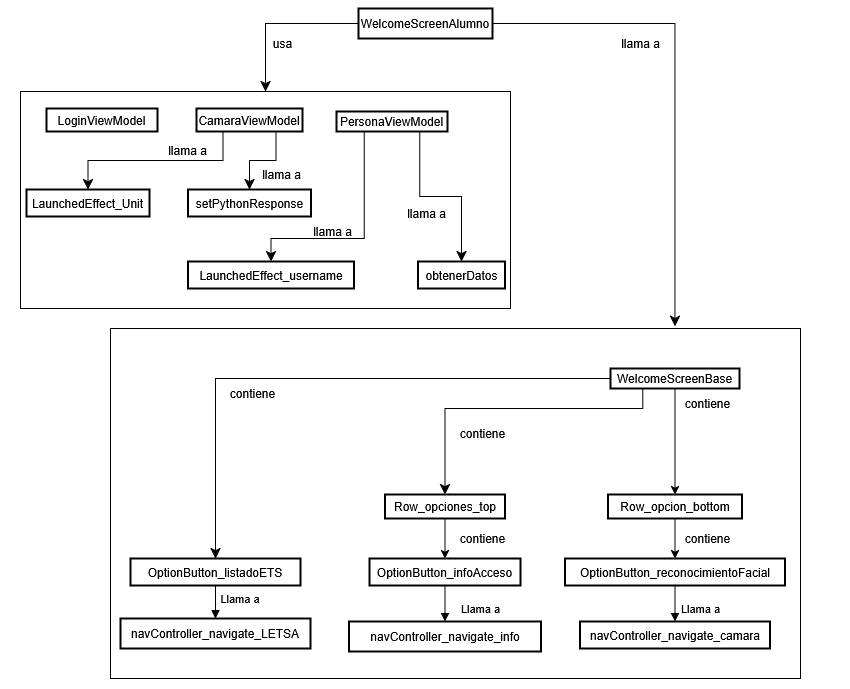
\includegraphics[width=0.9\textwidth]{DiagramasMoviles/DCM (35)}
		\caption{Diagrama de componentes para WelcomeScreenAlumno.kt .}
		\label{fig:Componentes_22}
	\end{center}
\end{figure}

\newpage

\subsection{Diagrama de Componentes de WelcomeScreenDocente.kt}

La Figura \ref{fig:Componentes_23} muestra el diagrama de componentes para WelcomeScreenDocente.kt que es un composable que contiene a la pantalla \IUref{IUE01}{Pantalla saludo de docente}, que es la pantalla de inicio del Docente (donde pude seleccionar la operación que quiere realizar y ver un saludo con su nombre).

\begin{figure}[htbp!]
	\begin{center}
		\includegraphics[width=0.9\textwidth]{DiagramasMoviles/DCM (36)}
		\caption{Diagrama de componentes para WelcomeScreenDocente.kt .}
		\label{fig:Componentes_23}
	\end{center}
\end{figure}

\newpage


%\section{Diagrama de clases}

%En la figura \ref{fig:Diagrama de clases} se muestra el diagrama de clases del sistema, en el cual se establecen las clases que tenemos contempladas para ser implementadas en la creación del sistema, a su vez en este se muestran las relaciones entre las clases, los atributos que estes clases contienen y los procesos que llevaran a cabo.


%\begin{figure}[htbp!]
%	\begin{center}
%		\includegraphics[width=1\textwidth]{Clases/Clases2}
%		\caption{Diagrama de clases.}
%		\label{fig:Diagrama de clases}
%	\end{center}
%\end{figure}


\section{Diagramas de secuencia}

A continuación, se presentan los diagramas de secuencia identificados para para la propuesta de solución presentada en este documento.
En ellos se busca ilustrar el funcionamiento dinamico del sistema y modelar las interacciones entre los distintos componentes y actores dependiendo de los casos de uso descritos en el capitulo 4. 
Cada diagrama representa el flujo de mensajes e información entre los actores y las capas de la aplicación en función de la arquitectura de una aplicación basada en Spring boot.

\subsection{SE-01 Iniciar sesión del sistema móvil}

\begin{figure}[htbp!]
	\begin{center}
		\fbox{\includegraphics[width=1\textwidth]{Secuencia/CU-01.png}}
		\caption{Diagrama de secuencia del caso de uso número 01 (Iniciar sesión del sistema móvil).}
		\label{fig:Diagrama de secuencia CU-01}
	\end{center}
\end{figure}

En el diagrama de secuencia \ref{fig:Diagrama de secuencia CU-01} de secuencia se describe el proceso planeado para el caso de uso \hyperlink{CU-01}{CU-01 Iniciar sesión del sistema móvil}, mostrando las interacciones que tendrá con la vista, el controlador, el servicio, el repositorio y la base de datos.

\newpage

\subsection{SE-02 Consultar calendario escolar}

\begin{figure}[htbp!]
	\begin{center}
		\fbox{\includegraphics[width=1\textwidth]{Secuencia/CU-02.png}}
		\caption{Diagrama de secuencia del caso de uso número 02 (Consultar calendario escolar).}
		\label{fig:Diagrama de secuencia CU-02}
	\end{center}
\end{figure}

En el diagrama de secuencia \ref{fig:Diagrama de secuencia CU-02} se describe el proceso planeado para el caso de uso \hyperlink{CU-02}{CU-02 Consultar calendario escolar}, mostrando las interacciones que tendrá con la vista, el controlador, el servicio, el repositorio y la base de datos.

\newpage

\subsection{SE-03 Consultar notificaciones}

\begin{figure}[htbp!]
	\begin{center}
		\fbox{\includegraphics[width=1\textwidth]{Secuencia/CU-03.png}}
		\caption{Diagrama de secuencia del caso de uso número 03 (Consultar notificaciones).}
		\label{fig:Diagrama se secuencia CU-03}
	\end{center}
\end{figure}

En el diagrama de secuencia \ref{fig:Diagrama de secuencia CU-03} se describe el proceso planeado para el caso de uso \hyperlink{CU-03}{CU-03 Consultar notificaciones}, mostrando las interacciones que tendrá con la vista, el controlador, el servicio, el repositorio y la base de datos.

\newpage

\subsection{SE-04 Consultar periodos de ETS asignados al docente}

\begin{figure}[htbp!]
	\begin{center}
		\fbox{\includegraphics[width=1\textwidth]{Secuencia/CU-04.png}}
		\caption{Diagrama de secuencia del caso de uso número 04 (Consultar periodos de ETS asignados al docente).}
		\label{fig:Diagrama de secuencia CU-04}
	\end{center}
\end{figure}

En el diagrama de secuencia \ref{fig:Diagrama de secuencia CU-04} se describe el proceso planeado para el caso de uso \hyperlink{CU-04}{CU-04 Consultar periodos de ETS asignados al docente}, mostrando las interacciones que tendrá con la vista, el controlador, el servicio, el repositorio y la base de datos.

\newpage

\subsection{SE-05 Consultar ETS asignados}

\begin{figure}[htbp!]
	\begin{center}
		\fbox{\includegraphics[width=1\textwidth]{Secuencia/CU-05.png}}
		\caption{Diagrama de secuencia del caso de uso número 05 (Consultar ETS asignados).}
		\label{fig:Diagrama de secuencia CU-05}
	\end{center}
\end{figure}

En el diagrama de secuencia \ref{fig:Diagrama de secuencia CU-05} se describe el proceso planeado para el caso de uso \hyperlink{CU-05}{CU-05 Consultar ETS asignados}, mostrando las interacciones que tendrá con la vista, el controlador, el servicio, el repositorio y la base de datos.

\newpage

\subsection{SE-06 Mostrar información de los ETS asignados}

\begin{figure}[htbp!]
	\begin{center}
		\fbox{\includegraphics[width=1\textwidth]{Secuencia/CU-06.png}}
		\caption{Diagrama de secuencia del caso de uso número 06 (Mostrar información de los ETS asignados).}
		\label{fig:Diagrama de secuencia CU-06}
	\end{center}
\end{figure}

En el diagrama de secuencia \ref{fig:Diagrama de secuencia CU-06} se describe el proceso planeado para el caso de uso \hyperlink{CU-06}{CU-06 Mostrar información de los ETS asignados}, mostrando las interacciones que tendrá con la vista, el controlador, el servicio, el repositorio y la base de datos.

\newpage

\subsection{SE-07 Solicitar remplazo}

\begin{figure}[htbp!]
	\begin{center}
		\fbox{\includegraphics[width=1\textwidth]{Secuencia/CU-07.png}}
		\caption{Diagrama de secuencia del caso de uso número 07 (Solicitar remplazo).}
		\label{fig:Diagrama de secuencia CU-07}
	\end{center}
\end{figure}

En el diagrama de secuencia \ref{fig:Diagrama de secuencia CU-07} se describe el proceso planeado para el caso de uso \hyperlink{CU-07}{CU-07 Solicitar remplazo}, mostrando las interacciones que tendrá con la vista, el controlador, el servicio, el repositorio y la base de datos.

\newpage

\subsection{SE-08 Consultar lista de alumnos inscritos a un ETS}

\begin{figure}[htbp!]
	\begin{center}
		\fbox{\includegraphics[width=1\textwidth]{Secuencia/CU-08.png}}
		\caption{Diagrama de secuencia del caso de uso número 08 (Consultar lista de alumnos inscritos a un ETS).}
		\label{fig:Diagrama de secuencia CU-08}
	\end{center}
\end{figure}

En el diagrama de secuencia \ref{fig:Diagrama de secuencia CU-08} se describe el proceso planeado para el caso de uso \hyperlink{CU-08}{CU-08 Consultar lista de alumnos inscritos a un ETS}, mostrando las interacciones que tendrá con la vista, el controlador, el servicio, el repositorio y la base de datos.

\newpage

\subsection{SE-09 Tomar asistencias a los ETS}

\begin{figure}[htbp!]
	\begin{center}
		\fbox{\includegraphics[width=.7\textwidth]{Secuencia/CU-09.png}}
		\caption{Diagrama de secuencia del caso de uso número 09 (Tomar asistencias a los ETS).}
		\label{fig:Diagrama de secuencia CU-09}
	\end{center}
\end{figure}

En el diagrama de secuencia \ref{fig:Diagrama de secuencia CU-09} se describe el proceso planeado para el caso de uso \hyperlink{CU-09}{CU-09 Tomar asistencias a los ETS}, mostrando las interacciones que tendrá con la vista, el controlador, el servicio, el repositorio y la base de datos.

\subsection{SE-10 Consultar lista de asistencia de alumnos inscritos a los ETS}

\begin{figure}[htbp!]
	\begin{center}
		\fbox{\includegraphics[width=1\textwidth]{Secuencia/CU-10.png}}
		\caption{Diagrama de secuencia del caso de uso número 10 (Consultar lista de asistencia de alumnos inscritos a los ETS).}
		\label{fig:Diagrama de secuencia CU-10}
	\end{center}
\end{figure}

En el diagrama de secuencia \ref{fig:Diagrama de secuencia CU-10} se describe el proceso planeado para el caso de uso \hyperlink{CU-10}{CU-10 Consultar lista de asistencia de alumnos inscritos a los ETS}, mostrando las interacciones que tendrá con la vista, el controlador, el servicio, el repositorio y la base de datos.

\newpage

\subsection{SE-11 Mostrar la foto e información  del alumno}

\begin{figure}[htbp!]
	\begin{center}
		\fbox{\includegraphics[width=1\textwidth]{Secuencia/CU-11.png}}
		\caption{Diagrama de secuencia del caso de uso número 11 (Mostrar la foto e información  del alumno).}
		\label{fig:Diagrama de secuencia CU-11}
	\end{center}
\end{figure}


En el diagrama de secuencia \ref{fig:Diagrama de secuencia CU-11} se describe el proceso planeado para el caso de uso \hyperlink{CU-11}{CU-11 Mostrar la foto e información  del alumno}, mostrando las interacciones que tendrá con la vista, el controlador, el servicio, el repositorio y la base de datos.

\newpage

\subsection{SE-12 Consultar alumno mediante código QR de la credencial}

\begin{figure}[htbp!]
	\begin{center}
		\fbox{\includegraphics[width=1\textwidth]{Secuencia/CU-12.png}}
		\caption{Diagrama de secuencia del caso de uso número 12 (Consultar alumno mediante código QR de la credencial).}
		\label{fig:Diagrama de secuencia CU-12}
	\end{center}
\end{figure}

En el diagrama de secuencia \ref{fig:Diagrama de secuencia CU-12} se describe el proceso planeado para el caso de uso \hyperlink{CU-12}{CU-12 Consultar alumno mediante código QR de la credencial}, mostrando las interacciones que tendrá con la vista, el controlador, el servicio, el repositorio y la base de datos.

\newpage

\subsection{SE-13 Buscar alumno por boleta}

\begin{figure}[htbp!]
	\begin{center}
		\fbox{\includegraphics[width=1\textwidth]{Secuencia/CU-13.png}}
		\caption{Diagrama de secuencia del caso de uso número 13 (Buscar alumno por boleta).}
		\label{fig:Diagrama de secuencia CU-13}
	\end{center}
\end{figure}

En el diagrama de secuencia \ref{fig:Diagrama de secuencia CU-13} se describe el proceso planeado para el caso de uso \hyperlink{CU-13}{CU-13 Buscar alumno por boleta}, mostrando las interacciones que tendrá con la vista, el controlador, el servicio, el repositorio y la base de datos.

\newpage

\subsection{SE-14 Buscar alumno por nombre}

\begin{figure}[htbp!]
	\begin{center}
		\fbox{\includegraphics[width=1\textwidth]{Secuencia/CU-14.png}}
		\caption{Diagrama de secuencia del caso de uso número 14 (Buscar alumno por nombre).}
		\label{fig:Diagrama de secuencia CU-14}
	\end{center}
\end{figure}

En el diagrama de secuencia \ref{fig:Diagrama de secuencia CU-14} se describe el proceso planeado para el caso de uso \hyperlink{CU-14}{CU-14 Buscar alumno por nombre}, mostrando las interacciones que tendrá con la vista, el controlador, el servicio, el repositorio y la base de datos.

\newpage

\subsection{SE-15 Registrar asistencia}

\begin{figure}[htbp!]
	\begin{center}
		\fbox{\includegraphics[width=.7\textwidth]{Secuencia/CU-15.png}}
		\caption{Diagrama de secuencia del caso de uso número 15 (Registrar asistencia).}
		\label{fig:Diagrama de secuencia CU-15}
	\end{center}
\end{figure}

En el diagrama de secuencia \ref{fig:Diagrama de secuencia CU-15} se describe el proceso planeado para el caso de uso \hyperlink{CU-15}{CU-15 Registrar asistencia}, mostrando las interacciones que tendrá con la vista, el controlador, el servicio, el repositorio y la base de datos.

\subsection{SE-16 Consultar periodos de ETS inscritos del alumno}

\begin{figure}[htbp!]
	\begin{center}
		\fbox{\includegraphics[width=1\textwidth]{Secuencia/CU-16.png}}
		\caption{Diagrama de secuencia del caso de uso número 16 (Consultar periodos de ETS inscritos del alumno).}
		\label{fig:Diagrama de secuencia CU-16}
	\end{center}
\end{figure}

En el diagrama de secuencia \ref{fig:Diagrama de secuencia CU-16} se describe el proceso planeado para el caso de uso \hyperlink{CU-16}{CU-16 Consultar periodos de ETS inscritos del alumno}, mostrando las interacciones que tendrá con la vista, el controlador, el servicio, el repositorio y la base de datos.

\newpage

\subsection{SE-17 Consultar ETS inscritos}

\begin{figure}[htbp!]
	\begin{center}
		\fbox{\includegraphics[width=1\textwidth]{Secuencia/CU-17.png}}
		\caption{Diagrama de secuencia del caso de uso número 04 (Consultar ETS inscritos).}
		\label{fig:Diagrama de secuencia CU-17}
	\end{center}
\end{figure}

En el diagrama de secuencia \ref{fig:Diagrama de secuencia CU-17} se describe el proceso planeado para el caso de uso \hyperlink{CU-17}{CU-17 Consultar  ETS inscritos}, mostrando las interacciones que tendrá con la vista, el controlador, el servicio, el repositorio y la base de datos.

\newpage

\subsection{SE-18 Mostrar información del los ETS inscritos}

\begin{figure}[htbp!]
	\begin{center}
		\fbox{\includegraphics[width=1\textwidth]{Secuencia/CU-18.png}}
		\caption{Diagrama de secuencia del caso de uso número 18 (Mostrar información del los ETS inscritos).}
		\label{fig:Diagrama de secuencia CU-18}
	\end{center}
\end{figure}

En el diagrama de secuencia \ref{fig:Diagrama de secuencia CU-18} se describe el proceso planeado para el caso de uso \hyperlink{CU-18}{CU-18 Mostrar información del los ETS inscritos}, mostrando las interacciones que tendrá con la vista, el controlador, el servicio, el repositorio y la base de datos.

\newpage

\subsection{SE-19 Probar reconocimiento facial}

\begin{figure}[htbp!]
	\begin{center}
		\fbox{\includegraphics[width=1\textwidth]{Secuencia/CU-19.png}}
		\caption{Diagrama de secuencia del caso de uso número 19 (Probar reconocimiento facial).}
		\label{fig:Diagrama de secuencia CU-19}
	\end{center}
\end{figure}

En el diagrama de secuencia \ref{fig:Diagrama de secuencia CU-19} se describe el proceso planeado para el caso de uso \hyperlink{CU-19}{CU-19 Probar reconocimiento facial}, mostrando las interacciones que tendrá con la vista, el controlador, el servicio, el repositorio y la base de datos.

\newpage

\subsection{SE-20 Revisar información de acceso a los ETS}

\begin{figure}[htbp!]
	\begin{center}
		\fbox{\includegraphics[width=1\textwidth]{Secuencia/CU-20.png}}
		\caption{Diagrama de secuencia del caso de uso número 20 (Revisar información de acceso a los ETS).}
		\label{fig:Diagrama de secuencia CU-20}
	\end{center}
\end{figure}

En el diagrama de secuencia \ref{fig:Diagrama de secuencia CU-20} se describe el proceso planeado para el caso de uso \hyperlink{CU-20}{CU-20 Revisar información de acceso a los ETS}, mostrando las interacciones que tendrá con la vista, el controlador, el servicio, el repositorio y la base de datos.

\newpage

\subsection{SE-21 Dar de alta a alumno}

\begin{figure}[htbp!]
	\begin{center}
		\fbox{\includegraphics[width=1\textwidth]{Secuencia/CU-21.png}}
		\caption{Diagrama de secuencia del caso de uso número 21 (Dar de alta a alumno).}
		\label{fig:Diagrama de secuencia CU-21}
	\end{center}
\end{figure}

En el diagrama de secuencia \ref{fig:Diagrama de secuencia CU-21} se describe el proceso planeado para el caso de uso \hyperlink{CU-21}{CU-21 Dar de alta a alumno}, mostrando las interacciones que tendrá con la vista, el controlador, el servicio, el repositorio y la base de datos.

\newpage

\subsection{SE-22 Crear credencial y capturar fotografía estudiantil}

\begin{figure}[htbp!]
	\begin{center}
		\fbox{\includegraphics[width=1\textwidth]{Secuencia/CU-22_23.png}}
		\caption{Diagrama de secuencia del caso de uso número 22 y 23 (Crear credencial y capturar fotografía estudiantil).}
		\label{fig:Diagrama de secuencia CU-22 y CU23}
	\end{center}
\end{figure}

En el diagrama de secuencia \ref{fig:Diagrama de secuencia CU-22 y CU23} y se describe el proceso planeado para el caso de uso \hyperlink{CU-22}{CU-22 Crear credencia} y \hyperlink{CU-23}{CU-23 Capturar fotografía estudiantil}, mostrando las interacciones que tendrá con la vista, el controlador, el servicio, el repositorio y la base de datos.

\newpage

\subsection{SE-23 Consultar lista de periodo de ETS}

\begin{figure}[htbp!]
	\begin{center}
		\fbox{\includegraphics[width=1\textwidth]{Secuencia/CU-24.png}}
		\caption{Diagrama de secuencia del caso de uso número 24 (Consultar lista de periodo de ETS).}
		\label{fig:Diagrama de secuencia CU-24}
	\end{center}
\end{figure}

En el diagrama de secuencia \ref{fig:Diagrama de secuencia CU-24} se describe el proceso planeado para el caso de uso \hyperlink{CU-24}{CU-24 Consultar lista de periodo de ETS}, mostrando las interacciones que tendrá con la vista, el controlador, el servicio, el repositorio y la base de datos.

\newpage

\subsection{SE-24 Dar de alta de periodo de ETS}

\begin{figure}[htbp!]
	\begin{center}
		\fbox{\includegraphics[width=1\textwidth]{Secuencia/CU-25.png}}
		\caption{Diagrama de secuencia del caso de uso número 25 (Dar de alta de periodo de ETS).}
		\label{fig:Diagrama de secuencia CU-25}
	\end{center}
\end{figure}

En el diagrama de secuencia \ref{fig:Diagrama de secuencia CU-25} se describe el proceso planeado para el caso de uso \hyperlink{CU-25}{CU-25 Dar de alta de periodo de ETS}, mostrando las interacciones que tendrá con la vista, el controlador, el servicio, el repositorio y la base de datos.

\newpage

\subsection{SE-25 Consultar lista de ETS}

\begin{figure}[htbp!]
	\begin{center}
		\fbox{\includegraphics[width=1\textwidth]{Secuencia/CU-28.png}}
		\caption{Diagrama de secuencia del caso de uso número 28 (Consultar lista de ETS).}
		\label{fig:Diagrama de secuencia CU-28}
	\end{center}
\end{figure}

En el diagrama de secuencia \ref{fig:Diagrama de secuencia CU-28} se describe el proceso planeado para el caso de uso \hyperlink{CU-28}{CU-28 Consultar lista de ETS}, mostrando las interacciones que tendrá con la vista, el controlador, el servicio, el repositorio y la base de datos.

\newpage

\subsection{SE-26 Dar de alta ETS}

\begin{figure}[htbp!]
	\begin{center}
		\fbox{\includegraphics[width=1\textwidth]{Secuencia/CU-29.png}}
		\caption{Diagrama de secuencia del caso de uso número 29 (Dar de alta ETS).}
		\label{fig:Diagrama de secuencia CU-29}
	\end{center}
\end{figure}

En el diagrama de secuencia \ref{fig:Diagrama de secuencia CU-29} se describe el proceso planeado para el caso de uso \hyperlink{CU-29}{CU-29 Dar de alta ETS}, mostrando las interacciones que tendrá con la vista, el controlador, el servicio, el repositorio y la base de datos.

\newpage

\subsection{SE-27 Consultar lista de personal de seguridad}

\begin{figure}[htbp!]
	\begin{center}
		\fbox{\includegraphics[width=1\textwidth]{Secuencia/CU-32.png}}
		\caption{Diagrama de secuencia del caso de uso número 32 (Consultar lista de personal de seguridad).}
		\label{fig:Diagrama de secuencia CU-32}
	\end{center}
\end{figure}

En el diagrama de secuencia \ref{fig:Diagrama de secuencia CU-32} se describe el proceso planeado para el caso de uso \hyperlink{CU-32}{CU-32 Consultar lista de personal de seguridad}, mostrando las interacciones que tendrá con la vista, el controlador, el servicio, el repositorio y la base de datos.

\newpage

\subsection{SE-28 Dar de alta personal de seguridad}

\begin{figure}[htbp!]
	\begin{center}
		\fbox{\includegraphics[width=1\textwidth]{Secuencia/CU-33.png}}
		\caption{Diagrama de secuencia del caso de uso número 33 (Dar de alta personal de seguridad).}
		\label{fig:Diagrama de secuencia CU-33}
	\end{center}
\end{figure}

En el diagrama de secuencia \ref{fig:Diagrama de secuencia CU-33} se describe el proceso planeado para el caso de uso \hyperlink{CU-33}{CU-33 Dar de alta personal de seguridad}, mostrando las interacciones que tendrá con la vista, el controlador, el servicio, el repositorio y la base de datos.

\newpage

\subsection{SE-29 Consultar lista de docentes}

\begin{figure}[htbp!]
	\begin{center}
		\fbox{\includegraphics[width=1\textwidth]{Secuencia/CU-36.png}}
		\caption{Diagrama de secuencia del caso de uso número 36 (Consultar lista de docentes).}
		\label{fig:Diagrama de secuencia CU-36}
	\end{center}
\end{figure}

En el diagrama de secuencia \ref{fig:Diagrama de secuencia CU-36} se describe el proceso planeado para el caso de uso \hyperlink{CU-36}{CU-36 Consultar lista de docentes}, mostrando las interacciones que tendrá con la vista, el controlador, el servicio, el repositorio y la base de datos.

\newpage

\subsection{SE-30 Dar de alta docente}

\begin{figure}[htbp!]
	\begin{center}
		\fbox{\includegraphics[width=1\textwidth]{Secuencia/CU-37.png}}
		\caption{Diagrama de secuencia del caso de uso número 37 (Dar de alta docente).}
		\label{fig:Diagrama de secuencia CU-37}
	\end{center}
\end{figure}

En el diagrama de secuencia \ref{fig:Diagrama de secuencia CU-37} se describe el proceso planeado para el caso de uso \hyperlink{CU-37}{CU-37 Dar de alta docente}, mostrando las interacciones que tendrá con la vista, el controlador, el servicio, el repositorio y la base de datos.

\newpage

\subsection{SE-31 Solicitar desbloqueo de cuenta}

\begin{figure}[htbp!]
	\begin{center}
		\fbox{\includegraphics[width=1\textwidth]{Secuencia/CU-40.png}}
		\caption{Diagrama de secuencia del caso de uso número 40 (Solicitar desbloqueo de cuenta).}
		\label{fig:Diagrama de secuencia CU-40}
	\end{center}
\end{figure}

En el diagrama de secuencia \ref{fig:Diagrama de secuencia CU-40} se describe el proceso planeado para el caso de uso \hyperlink{CU-40}{CU-40 Solicitar desbloqueo de cuenta}, mostrando las interacciones que tendrá con la vista, el controlador, el servicio, el repositorio y la base de datos.

\newpage

\subsection{SE-32 Iniciar sesión del sistema web}

\begin{figure}[htbp!]
	\begin{center}
		\fbox{\includegraphics[width=1\textwidth]{Secuencia/CU-41.png}}
		\caption{Diagrama de secuencia del caso de uso número 41 (Iniciar sesión del sistema web).}
		\label{fig:Diagrama de secuencia CU-41}
	\end{center}
\end{figure}


En el diagrama de secuencia \ref{fig:Diagrama de secuencia CU-41} se describe el proceso planeado para el caso de uso \hyperlink{CU-41}{CU-41 Iniciar sesión del sistema web}, mostrando las interacciones que tendrá con la vista, el controlador, el servicio, el repositorio y la base de datos.

\newpage

\subsection{SE-33 Asignar docente de remplazo}

\begin{figure}[htbp!]
	\begin{center}
		\fbox{\includegraphics[width=1\textwidth]{Secuencia/CU-42.png}}
		\caption{Diagrama de secuencia del caso de uso número 42 (Asignar docente de remplazo).}
		\label{fig:Diagrama de secuencia CU-42}
	\end{center}
\end{figure}

En el diagrama de secuencia \ref{fig:Diagrama de secuencia CU-42} se describe el proceso planeado para el caso de uso \hyperlink{CU-42}{CU-42 Asignar docente de remplazo}, mostrando las interacciones que tendrá con la vista, el controlador, el servicio, el repositorio y la base de datos.


\chapter{Trabajo futuro}

En este capítulo se mencionará lo que se tiene planeado realizar para el siguiente periodo de TT en ella se describen las actividades que se debe realizar para el funcionamiento del sistema, además se mencionan algunas mejoras que se deben realizar

Para la implementación del backend, se utilizará Spring Boot como framework principal, permitiendo establecer una comunicación eficiente entre Kotlin y la base de datos. Se aprovecharán las diversas herramientas que ofrece Spring Boot, para facilitar la interacción con la base de datos y gestionar las operaciones. 
Ahora bien, para la implementación de la base de datos se utilizará PostgreSQL como sistema gestor de base de datos.

Por otro lado, para el desarrollo de la parte móvil se planea desarrollar una serie de puntos:
\begin{itemize}
    
    \item Implementar canales seguros DE HTTP para el intercambio de datos sensibles. 
    \item Optimizacion de métodos de lista y repositorio para mejorar el rendimiento en consultas. 
    \item Implementación de un módulo para que Kotlin envíe imágenes directamente a la BD. 
    \item Programar las pantallas del sistema. 
    \item un módulo de notificación qué permitirá a los usuarios mantener a los usuarios informados sobre las modificaciones que puedan surgir en los ETS. 
    \item Implementar un esquema de encriptacion de datos para la protección de datos.
\end{itemize}

Finalmente, con los resultados obtenidos en esta primera parte del trabajo terminal se buscará mejorar el modelo de extracción de características para la generación de embeddings que permitan realizar la identificación de usuarios siguiendo un enfoque de verificación, esto permitirá la creación de una base de datos vectorial persistente para finalmente implementar el proceso de inferencia/reconocimiento en tiempo real.

%=========================================================
\chapter{Pruebas}

El aseguramiento de la calidad es un pilar fundamental en el desarrollo de cualquier sistema de software. En el presente capítulo, se detalla el proceso de validación del sistema propuesto a través de la ejecución de pruebas enfocadas en sus principales casos de uso. El objetivo es verificar que cada funcionalidad crucial del sistema se comporta de acuerdo con las especificaciones y requisitos definidos. 

Para cada caso de uso evaluado, se presentará un informe detallado que incluye la descripción del caso de prueba, los supuestos y condiciones previas necesarias para su ejecución, los datos de prueba utilizados, los pasos específicos a ejecutar, el resultado esperado y el resultado real obtenido. Asimismo, se documentarán los errores detectados, si los hubo, y el estado final de la prueba. Esta metodología permite una revisión exhaustiva del comportamiento del sistema frente a las interacciones clave de los usuarios. 



\section{Caso de prueba CP01 - Inicio de sesión de la app móvil}

\begin{longtable}{|p{5cm}|p{10cm}|}
	\hline
	\multicolumn{2}{|c|}{\textbf{CASO DE PRUEBA - CP01 Inicio de sesión de la app móvil}} \\
	\hline
	\textbf{Caso de uso relacionado} & \hyperref[CU-01]{CU-01 Inicio de sesión de la app móvil} \\
	\hline
	\textbf{Descripción} & Validar la funcionalidad del inicio de sesión para todos los usuarios registrados dentro del sistema. \\
	\hline
	\textbf{Supuestos y Condiciones Previas} & 
	\begin{itemize}
		\item El usuario debe de haber instalado la aplicación en su celular.
		\item El usuario debe de estar registrado en la base de datos.
	\end{itemize} \\
	\hline
	\textbf{Datos de Prueba} & 
	\begin{itemize}
		\item Boleta en caso de ser alumno, RFC en caso de ser personal de seguridad o personal académico.
	\end{itemize} \\
	\hline
	\textbf{Pasos a Ejecutar} & 
	\begin{enumerate}
		\item Ingresar la boleta o RFC dependiendo del tipo de usuario, en el campo de usuario.
		\item Ingresar la boleta o RFC dependiendo del tipo de usuario, en el campo de contraseña.
		\item Presionar el botón `Entrar`.
	\end{enumerate} \\
	\hline
	\textbf{Resultado Esperado} & 
	Redirige al usuario a su pantalla principal. Dependiendo del tipo de usuario que sea, lo redirigirá a una pantalla específica en el que podrá seleccionar entre diferentes opciones a realizar. \\
	\hline
	\textbf{Errores Detectados} & 
	Ninguno. \\
	\hline
	\textbf{Resultado Real y Condiciones Posteriores} & 
	\begin{itemize}
		\item En caso de tener conexión a internet, el usuario es redirigido a su pantalla de inicio. En caso contrario, despliega un `Error de conexión`.
	\end{itemize} \\
	\hline
	\textbf{Estado} & 
	\textbf{Aprobado} - Si el logeo es exitoso, el usuario es redirigido a su pantalla de bienvenida específica.   \\
	\hline
\end{longtable}
%---------------------------------------------------------
%
\section{Caso de prueba CP001-Consultar alumno mediante código QR de la credencial}

\begin{longtable}{|p{5cm}|p{10cm}|}
	\hline
	\multicolumn{2}{|c|}{\textbf{CASO DE PRUEBA - CP001 Consultar alumno mediante código QR de la credencial}} \\
	\hline
	\textbf{ID del Caso de Prueba} & CP001- Consultar alumno mediante código QR de la credencial \\
	\hline
	\textbf{Descripción} & Validar la funcionalidad de obtención de la credencial del alumno mediante técnicas de scraping con Selenium, asegurando su compatibilidad tanto en entornos locales como en entornos de despliegue en la nube (Azure). \\
	\hline
	\textbf{Supuestos y Condiciones Previas} & 
	\begin{itemize}
		\item El personal de seguridad debe haber iniciado sesión en el sistema.
		\item El dispositivo debe contar con cámara funcional.
		\item La URL de la credencial debe ser accesible y válida.
	\end{itemize} \\
	\hline
	\textbf{Datos de Prueba} & 
	\begin{itemize}
		\item URL de la credencial del alumno.
	\end{itemize} \\
	\hline
	\textbf{Pasos a Ejecutar} & 
	\begin{enumerate}
		\item Iniciar sesión en la aplicación como personal de seguridad.
		\item Activar los permisos de la cámara del dispositivo para escanear el código QR.
		\item Escanear el código QR correspondiente a la credencial del alumno.
		\item Esperar la respuesta del sistema con la credencial renderizada.
		\item Verificar que se muestran correctamente los datos personales del alumno junto con la imagen de la credencial.
	\end{enumerate} \\
	\hline
	\textbf{Resultado Esperado} & 
	La credencial del alumno debe renderizarse correctamente y generar una imagen funcional, tanto en entorno local como en el entorno de producción. \\
	\hline
	\textbf{Resultado Real y Condiciones Posteriores} & 
	\begin{itemize}
		\item En entorno local: Selenium y Playwright funcionaron correctamente.
		\item En Azure: Selenium y Playwright presentaron fallos debido a incompatibilidades con dependencias nativas.
		\item Se implementó una solución alternativa utilizando la generación de PDF y su posterior conversión a imagen, la cual resultó funcional.
	\end{itemize} \\
	\hline
	\textbf{Estado} & 
	\textbf{Fallido} con Selenium/Playwright en Azure.  
	
	\textbf{Aprobado} con solución alternativa basada en PDF. \\
	\hline
\end{longtable}

\section{Caso de prueba CP02 - Consultar calendario escolar}

\begin{longtable}{|p{5cm}|p{10cm}|}
	\hline
	\multicolumn{2}{|c|}{\textbf{CASO DE PRUEBA - CP02 Consultar calendario escolar}} \\
	\hline
	\textbf{Caso de uso relacionado} & \hyperref[CU-02]{CU-02 Consultar calendario escolar} \\
	\hline
	\textbf{Descripción} & Validar la funcionalidad de la obtención del calendario escolar del IPN directamente de su página oficial, así como la visualización correcta del calendario en formato de imagen. Así también, validar la funcionalidad del cálculo de días faltantes para un periodo de ETS. \\
	\hline
	\textbf{Supuestos y Condiciones Previas} & 
	\begin{itemize}
		\item El usuario debió de haber iniciado sesión en el sistema.
		\item El usuario debió de ingresar a la pantalla \IUref{IU02}{Pantalla Consultar calendario escolar}
		\item El usuario debe de tener una buena conexión a internet.
	\end{itemize} \\
	\hline
	\textbf{Datos de Prueba} & 
	\begin{itemize}
		\item Ninguno.
	\end{itemize} \\
	\hline
	\textbf{Pasos a Ejecutar} & 
	\begin{enumerate}
		\item El usuario presiona el ícono del calendario que se encuentra en el menú inferior de la aplicación.
		\item El usuario presiona el botón `Calcular cuántos días faltan para el periodo de ETS`.
	\end{enumerate} \\
	\hline
	\textbf{Resultado Esperado} & 
	\begin{itemize}
		\item Visualización de la imagen del calendario escolar actual del IPN. 
		\item Mensaje de los días faltantes para el periodo de ETS, si este ya pasó o si se encuentra en uno.
	\end{itemize}
	\\
	\hline
	\textbf{Errores Detectados} & 
	El mensaje no informaba al usuario si, de acuerdo a la fecha actual, se encontraba en un periodo de ETS. \\
	\hline
	\textbf{Resultado Real y Condiciones Posteriores} & 
	\begin{itemize}
		\item El sistema le informaba al usuario que el periodo de ETS ya había pasado apesar de que se encontraba en un periodo actual.
		\item El sistema no reconocía si había dos periodos de ETS dentro de un mismo periodo escolar.
		\item Se realizó un ajuste en la lógica del negocio para que devolviera mensajes más específicos y un cambio en la consulta para que reconociera los dos periodos de ETS.
	\end{itemize} \\
	\hline
	\textbf{Estado} & 
	\textbf{Aprobado} - El error fue corregido y la funcionalidad opera correctamente.   \\
	\hline
\end{longtable}
%---------------------------------------------------------
\section{Caso de prueba CP005 - Consultar ETS asignados}

\begin{longtable}{|p{5cm}|p{10cm}|}
	\hline
	\multicolumn{2}{|c|}{\textbf{CASO DE PRUEBA - CP005 Consultar ETS asignados}} \\
	\hline
	\textbf{ID del Caso de Prueba} & CP005 - Consultar ETS asignados \\
	\hline
	\textbf{Descripción} & Validar que el docente pueda consultar todos lo ETS y los ETS que tiene que aplicar . \\
	\hline
	\textbf{Supuestos y Condiciones Previas} & 
	\begin{itemize}
		\item El docente ha iniciado sesión en el sistema.
		\item Existen ETS asignados al docente.
		\item Existen ETS dados de alta.
	\end{itemize} \\
	\hline
	\textbf{Datos de Prueba} & 
	\begin{itemize}
		\item nombre de usuario del docente.
		\item Lista de ETS dados de alta.
	\end{itemize} \\
	\hline
	\textbf{Pasos a Ejecutar} & 
	\begin{enumerate}
		\item Iniciar sesión como docente.
		\item Seleccionar la opción ´´ETS´´ desde el menú.
	\end{enumerate} \\
	\hline
	\textbf{Resultado Esperado} & 
	Los ETS que están dados de alta se mostraran en pantalla. \\
	\hline
	\textbf{Errores Detectados} & 
	\begin{itemize}
		\item Para el filtro de ETS, mas específicamente el de `Mis ETS` no se mostraba ningún ETS.

	\end{itemize} \\
	\hline
	\textbf{Resultado Real y Condiciones Posteriores} & 
	\begin{itemize}
		\item Se modifico la lógica del envió de la solicitud de obtención los ETS para que devolvieran otra variable en la que se especificasen los ETS que el usuario tenía asignados.
		\item Se verificó el correcto funcionamiento tanto en base de datos como en la interfaz.
	\end{itemize} \\
	\hline
	\textbf{Estado} & 
	\textbf{Aprobado} - El error fue corregido y la funcionalidad opera correctamente. \\
	\hline
\end{longtable}
%---------------------------------------------------------
\section{Caso de prueba CP06 - Mostrar información de los ETS asignados}

\begin{longtable}{|p{5cm}|p{10cm}|}
	\hline
	\multicolumn{2}{|c|}{\textbf{CASO DE PRUEBA - CP06 Mostrar información de los ETS asignados}} \\
	\hline
	\textbf{Caso de uso relacionado} & \hyperref[CU-06]{CU-06 Mostrar información de los ETS asignados} \\
	\hline
	\textbf{Descripción} & Validar que el docente pueda revisar los datos específicos del ETS seleccionado. \\
	\hline
	\textbf{Supuestos y Condiciones Previas} & 
	\begin{itemize}
		\item El docente ha iniciado sesión en el sistema.
		\item Existen ETS dados de alta.
		\item El docente eligió un ETS.
		\item Hay información del ETS seleccionado.
	\end{itemize} \\
	\hline
	\textbf{Datos de Prueba} & 
	\begin{itemize}
		\item El docente se le muestra los detalles de ETS asignado: tipo de ETS, unidad de aprendizaje, periodo, fecha, turno, cupo, duración, salones (con tipo de salón por cada salón), Hora.
	\end{itemize} \\
	\hline
	\textbf{Pasos a Ejecutar} & 
	\begin{enumerate}
		\item Iniciar sesión como docente.
		\item Seleccionar la opción ´´ETS´´ desde el menú.
		\item Elegir un ETS disponible en la lista.
		\item Dar clic en el ETS.
		\item Revisa los datos mostrados.
	\end{enumerate} \\
	\hline
	\textbf{Resultado Esperado} & 
	Se le muestra al docente los datos del ETS seleccionado. \\
	\hline
	\textbf{Errores Detectados} & 
	\begin{itemize}
		\item En ocasiones al cambiar rápido entre ETS la aplicación se cerraba abruptamente.
		
	\end{itemize} \\
	\hline
	\textbf{Resultado Real y Condiciones Posteriores} & 
	\begin{itemize}
		\item Se modifico el orden de obtención y asignación de los datos, para que nos aseguráramos que los datos fueran  obtenidos antes ser asignados a las variables (evitar asignación de null y/o datos vacíos).
		\item Se verificó el correcto funcionamiento tanto en base de datos como en la interfaz.
	\end{itemize} \\
	\hline
	\textbf{Estado} & 
	\textbf{Aprobado} - El error fue corregido y la funcionalidad opera correctamente. \\
	\hline
\end{longtable}
%---------------------------------------------------------
\section{Caso de prueba CP007 - Solicitar reemplazo de ETS}

\begin{longtable}{|p{5cm}|p{10cm}|}
	\hline
	\multicolumn{2}{|c|}{\textbf{CASO DE PRUEBA - CP007 Solicitar reemplazo de ETS}} \\
	\hline
	\textbf{ID del Caso de Prueba} & CP007 - Solicitar reemplazo de ETS \\
	\hline
	\textbf{Descripción} & Validar que el docente pueda solicitar un reemplazo para un ETS seleccionado, ingresando una razón. \\
	\hline
	\textbf{Supuestos y Condiciones Previas} & 
	\begin{itemize}
		\item El docente ha iniciado sesión en el sistema.
		\item Existen ETS asignados al docente.
		\item El botón "Solicitar reemplazo" se encuentra habilitado para los ETS disponibles.
	\end{itemize} \\
	\hline
	\textbf{Datos de Prueba} & 
	\begin{itemize}
		\item ETS asignado al docente con fecha activa.
		\item Texto de razón de la solicitud de reemplazo.
	\end{itemize} \\
	\hline
	\textbf{Pasos a Ejecutar} & 
	\begin{enumerate}
		\item Iniciar sesión como docente.
		\item Seleccionar la opción ´´ETS´´ desde el menú.
		\item Elegir un ETS disponible en la lista.
		\item Dar clic en el botón “Solicitar reemplazo”.
		\item Ingresar la razón.
		\item Enviar la solicitud.
	\end{enumerate} \\
	\hline
	\textbf{Resultado Esperado} & 
	La solicitud de reemplazo debe registrarse exitosamente y mostrarse con el estatus “Pendiente”. \\
	\hline
	\textbf{Errores Detectados} & 
	\begin{itemize}
		\item Inicialmente, al enviar la solicitud, no se reflejaba el estatus de “Pendiente”.
		\item Se identificó un error en la lógica de actualización del estado posterior al envío.
	\end{itemize} \\
	\hline
	\textbf{Resultado Real y Condiciones Posteriores} & 
	\begin{itemize}
		\item Tras modificar la lógica de persistencia y actualización de estado en el backend, el sistema ahora registra correctamente la solicitud con estatus “Pendiente”.
		\item Se verificó el correcto funcionamiento tanto en base de datos como en la interfaz.
	\end{itemize} \\
	\hline
	\textbf{Estado} & 
	\textbf{Aprobado} - El error fue corregido y la funcionalidad opera correctamente. \\
	\hline
\end{longtable}

%---------------------------------------------------------
\section{Caso de prueba CP08 - Consultar lista de alumnos inscritos a un ETS}

\begin{longtable}{|p{5cm}|p{10cm}|}
	\hline
	\multicolumn{2}{|c|}{\textbf{CASO DE PRUEBA - CP08 Consultar lista de alumnos inscritos a un ETS}} \\
	\hline
	\textbf{Caso de uso relacionado} & \hyperref[CU-08]{CU-08 Consultar lista de alumnos inscritos a un ETS} \\
	\hline
	\textbf{Descripción} & Validar que el docente pueda revisar la lista de alumnos inscritos al ETS seleccionado. \\
	\hline
	\textbf{Supuestos y Condiciones Previas} & 
	\begin{itemize}
		\item El docente ha iniciado sesión en el sistema.
		\item Existen ETS dados de alta.
		\item El docente eligió un ETS.
		\item Hay información del ETS seleccionado.
		\item Hay alumnos inscritos al ETS.
		
	\end{itemize} \\
	\hline
	\textbf{Datos de Prueba} & 
	\begin{itemize}
		\item La lista de alumnos inscritos al ETS.
	\end{itemize} \\
	\hline
	\textbf{Pasos a Ejecutar} & 
	\begin{enumerate}
		\item Iniciar sesión como docente.
		\item Seleccionar la opción ´´ETS´´ desde el menú.
		\item Elegir un ETS disponible en la lista.
		\item Dar clic en el ETS.
		\item Revisa los datos mostrados.
		\item El docente elije la opcion ´´Ir a la lista de alumnos´´
		\item El docente revisa la lista de alumnos inscritos al ETS
	\end{enumerate} \\
	\hline
	\textbf{Resultado Esperado} & 
	Se le muestra al docente la lista de alumnos inscritos al ETS. \\	
	\hline
	\textbf{Errores Detectados} & 
	\begin{itemize}
		\item Ninguno.
		
	\end{itemize} \\
	\hline
	\textbf{Resultado Real y Condiciones Posteriores} & 
	\begin{itemize}

		\item Se verificó el correcto funcionamiento tanto en base de datos como en la interfaz.
	\end{itemize} \\
	\hline
	\textbf{Estado} & 
	\textbf{Aprobado} - la funcionalidad opera correctamente. \\
	\hline
\end{longtable}
%---------------------------------------------------------
\section{Caso de prueba CP009 - Tomar asistencias a los ETS}

\begin{longtable}{|p{5cm}|p{10cm}|}
	\hline
	\multicolumn{2}{|c|}{\textbf{CASO DE PRUEBA - CP009 Tomar asistencias a los ETS}} \\
	\hline
	\textbf{ID del Caso de Prueba} & CP009 - Tomar asistencias a los ETS \\
	\hline
	\textbf{Descripción} & Validar que el docente pueda crear reportes de asistencias e incidencias. \\
	\hline
	\textbf{Supuestos y Condiciones Previas} & 
	\begin{itemize}
		\item El docente ha iniciado sesión en el sistema.
		\item Existen ETS dados de alta.
		\item El docente eligió un ETS.
		\item Hay información del ETS seleccionado.
		\item Hay alumnos inscritos al ETS.
		
	\end{itemize} \\
	\hline
	\textbf{Datos de Prueba} & 
	\begin{itemize}
		\item razón, motivo y si se realiza reconocimiento facial; foto y precisión. 
	\end{itemize} \\
	\hline
	\textbf{Pasos a Ejecutar} & 
	\begin{enumerate}
		\item Iniciar sesión como docente.
		\item Seleccionar la opción ´´ETS´´ desde el menú.
		\item Elegir un ETS disponible en la lista.
		\item Dar clic en el ETS.
		\item Revisa los datos mostrados.
		\item El docente elije la opcion ´´Ir a la lista de alumnos´´
		\item El docente revisa la lista de alumnos inscritos al ETS
		\item El docente elige un alumno para crear un reporte de asistencia/incidencia.
	\end{enumerate} \\
	\hline
	\textbf{Resultado Esperado} & 
	Se crea el reporte correctamente. \\	
	\hline
	\textbf{Errores Detectados} & 
	\begin{itemize}
		\item Al tomar la foto para el reconocimiento facial en algunos dispositivos salia volteada y no dejaba que se realizara la correctamente el reconocimiento facial.
		\item Al mandar la imagen al servidor de la red neuronal, si la imagen es muy grande el servidor corta la conexión. 
		\item La imagen se estira si no se re escala correctamente y altera la información para el reconocimiento facial.
	\end{itemize} \\
	\hline
	\textbf{Resultado Real y Condiciones Posteriores} & 
	\begin{itemize}
		\item Para el error de la imagen volteada, e aplico un método que detecta la orientación de la foto y la rota al estado normal tomando en cuenta 0 grados como el estado de orientación correcto y dependiendo de la orientación se voltea hasta llegar a los 0 grados. 
		\item Para el error del tamaño al enviar al servidor se aplico un método de re escalado a un tamaño de 640 x 480 pixeles, esto después de la corrección de la orientación.
		\item Para el error de que la foto se estire, se realizo una escala entre las dimensiones de la foto para mantener esa escala al re dimensionar la foto.
		\item Se verificó el correcto funcionamiento tanto en base de datos como en la interfaz.
	\end{itemize} \\
	\hline
	\textbf{Estado} & 
	\textbf{Aprobado} - la funcionalidad opera correctamente. \\
	\hline
\end{longtable}
%---------------------------------------------------------
\section{Caso de prueba CP11 - Mostrar la foto e información del alumno}

\begin{longtable}{|p{5cm}|p{10cm}|}
	\hline
	\multicolumn{2}{|c|}{\textbf{CASO DE PRUEBA - CP11 Mostrar la foto e información del alumno}} \\
	\hline
	\textbf{Caso de uso relacionado} & \hyperref[CU-11]{CU-11 Mostrar la foto e información del alumno}\\
	\hline
	\textbf{Descripción} & Validar que el docente revisar los reportes creados por el o por otros docentes. \\
	\hline
	\textbf{Supuestos y Condiciones Previas} & 
	\begin{itemize}
		\item El docente ha iniciado sesión en el sistema.
		\item Existen ETS dados de alta.
		\item El docente eligió un ETS.
		\item Hay información del ETS seleccionado.
		\item Hay alumnos inscritos al ETS.
		
	\end{itemize} \\
	\hline
	\textbf{Datos de Prueba} & 
	\begin{itemize}
		\item Reporte. 
	\end{itemize} \\
	\hline
	\textbf{Pasos a Ejecutar} & 
	\begin{enumerate}
		\item Iniciar sesión como docente.
		\item Seleccionar la opción ´´ETS´´ desde el menú.
		\item Elegir un ETS disponible en la lista.
		\item Dar clic en el ETS.
		\item Revisa los datos mostrados.
		\item El docente elije la opción ´´Ir a la lista de alumnos´´
		\item El docente revisa la lista de alumnos inscritos al ETS
		\item El docente elige el reporte de un alumno.
	\end{enumerate} \\
	\hline
	\textbf{Resultado Esperado} & 
	El docente revisa el reporte. \\	
	\hline
	\textbf{Errores Detectados} & 
	\begin{itemize}
		\item La el dato de la hora y fecha de la creación del reporte salia mal por un error de tipos de datos.

	\end{itemize} \\
	\hline
	\textbf{Resultado Real y Condiciones Posteriores} & 
	\begin{itemize}
		\item Antes de mostrar la hora y la fecha son convertidos a un tipo de dato String.
		\item Se verificó el correcto funcionamiento tanto en base de datos como en la interfaz.
	\end{itemize} \\
	\hline
	\textbf{Estado} & 
	\textbf{Aprobado} - la funcionalidad opera correctamente. \\
	\hline
\end{longtable}
%---------------------------------------------------------

\section{Caso de prueba CP012 - Consultar alumno mediante código QR de la credencial}

\begin{longtable}{|p{5cm}|p{10cm}|}
	\hline
	\multicolumn{2}{|c|}{\textbf{CASO DE PRUEBA - CP012 Consultar alumno mediante código QR de la credencial}} \\
	\hline
	\textbf{ID del Caso de Prueba} & CP012 - Consultar alumno mediante código QR de la credencial \\
	\hline
	\textbf{Descripción} & Validar la funcionalidad de obtención de la credencial del alumno mediante técnicas de scraping con Selenium, asegurando su compatibilidad tanto en entornos locales como en entornos de despliegue en la nube (Azure). \\
	\hline
	\textbf{Supuestos y Condiciones Previas} & 
	\begin{itemize}
		\item El personal de seguridad debe haber iniciado sesión en el sistema.
		\item El dispositivo debe contar con cámara funcional.
		\item La URL de la credencial debe ser accesible y válida.
	\end{itemize} \\
	\hline
	\textbf{Datos de Prueba} & 
	\begin{itemize}
		\item URL de la credencial del alumno.
	\end{itemize} \\
	\hline
	\textbf{Pasos a Ejecutar} & 
	\begin{enumerate}
		\item Iniciar sesión en la aplicación como personal de seguridad.
		\item Activar los permisos de la cámara del dispositivo para escanear el código QR.
		\item Escanear el código QR correspondiente a la credencial del alumno.
		\item Esperar la respuesta del sistema con la credencial renderizada.
		\item Verificar que se muestran correctamente los datos personales del alumno junto con la imagen de la credencial.
	\end{enumerate} \\
	\hline
	\textbf{Resultado Esperado} & 
	La credencial del alumno debe renderizarse correctamente y generar una imagen funcional, tanto en entorno local como en el entorno de producción. \\
	\hline
	\textbf{Errores Detectados} &
	\begin{itemize}
		\item \textbf{Error 1:} Selenium y Playwright funcionaban correctamente en entorno local, pero fallaban en Azure.
		\item \textbf{Causa:} Incompatibilidades con dependencias nativas y configuración del entorno en la nube.
		\item \textbf{Solución:} Implementación de una solución alternativa basada en la generación de PDF de la credencial y su conversión a imagen.
	\end{itemize} \\
	\hline
	\textbf{Resultado Real y Condiciones Posteriores} & 
	\begin{itemize}
		\item En entorno local: Selenium y Playwright funcionaron correctamente.
		\item En Azure: Selenium y Playwright presentaron fallos debido a incompatibilidades con dependencias nativas.
		\item La solución alternativa basada en PDF generó una imagen funcional y compatible.
	\end{itemize} \\
	\hline
	\textbf{Estado} & 
	\textbf{Fallido} con Selenium/Playwright en Azure.  
	
	\textbf{Aprobado} con solución alternativa basada en PDF. \\
	\hline
\end{longtable}

%---------------------------------------------------------
\section{Caso de prueba CP13 - Consultar alumnos mediante búsqueda por boleta}

\begin{longtable}{|p{5cm}|p{10cm}|}
	\hline
	\multicolumn{2}{|c|}{\textbf{CASO DE PRUEBA - CP13 Consultar alumnos mediante búsqueda por boleta}} \\
	\hline
	\textbf{Caso de uso relacionado} & \hyperref[CU-13]{CU-13 Consultar alumnos mediante búsqueda por boleta} \\
	\hline
	\textbf{Descripción} & Validar la funcionalidad de consultar alumnos inscritos a un ETS, mediante búsqueda por número de boleta. \\
	\hline
	\textbf{Supuestos y Condiciones Previas} & 
	\begin{itemize}
		\item El personal de seguridad ha iniciado sesión correctamente.
		\item Existen alumnos inscritos a un ETS para la fecha consultada.
	\end{itemize} \\
	\hline
	\textbf{Datos de Prueba} & 
	\begin{itemize}
		\item Las boletas de los alumnos deberan ser válidas y deben estar inscritos en al menos un ETS.
		\item La fecha de consulta del ETS debe estar activa.
	\end{itemize} \\
	\hline
	\textbf{Pasos a Ejecutar} & 
	\begin{enumerate}
		\item Iniciar sesión como personal de seguridad.
		\item Seleccionar la opción " Consultar Alumnos" desde eñ menú.
		\item Ingresar el número de boleta en el buscador.
		\item Ejecutar la búsqueda y observar la lista de alumnos inscritos a ETS.
	\end{enumerate} \\
	\hline
	\textbf{Resultado Esperado} & 
	Los alumnos inscritos a un ETS en la fecha consultada y con la boleta ingresada deben mostrarse correctamente en la pantalla. \\
	\hline
	\textbf{Errores Detectados} &
	\begin{itemize}
		\item Inicialmente, no se mostraban alumnos al seleccionar "Consultar Alumnos" desde el menú.
		\item La lista de alumnos inscritos a ETS ese día aparecía vacía.
		\item Se verificó que la lógica de implementación no estaba retornando datos correctamente.
	\end{itemize} \\
	\hline
	\textbf{Resultado Real y Condiciones Posteriores} & 
	\begin{itemize}
		\item Tras corrección, el sistema mostró correctamente la lista de alumnos inscritos al ETS filtrada por boleta.
		\item Se validó que la consulta a la base de datos y el filtrado funcionaron correctamente.
	\end{itemize} \\
	\hline
	\textbf{Estado} & 
	\textbf{Aprobado} - El error fue corregido y la funcionalidad se encuentra funcionando. \\
	\hline
\end{longtable}
%---------------------------------------------------------
\section{Caso de prueba CP014 - Consultar alumnos mediante búsqueda por nombre}

\begin{longtable}{|p{5cm}|p{10cm}|}
	\hline
	\multicolumn{2}{|c|}{\textbf{CASO DE PRUEBA - CP014 Consultar alumnos mediante búsqueda por nombre}} \\
	\hline
	\textbf{ID del Caso de Prueba} & CP014 - Consultar alumnos mediante búsqueda por nombre \\
	\hline
	\textbf{Descripción} & Validar la funcionalidad de consultar alumnos inscritos a un ETS, mediante búsqueda por nombre. \\
	\hline
	\textbf{Supuestos y Condiciones Previas} & 
	\begin{itemize}
		\item El personal de seguridad ha iniciado sesión correctamente.
		\item Existen alumnos inscritos a un ETS para la fecha consultada.
	\end{itemize} \\
	\hline
	\textbf{Datos de Prueba} & 
	\begin{itemize}
		\item El nombre de los alumnos deberan ser válidas y deben estar inscritos en al menos un ETS.
		\item La fecha de consulta del ETS debe estar activa.
	\end{itemize} \\
	\hline
	\textbf{Pasos a Ejecutar} & 
	\begin{enumerate}
		\item Iniciar sesión como personal de seguridad.
		\item Seleccionar la opción " Consultar Alumnos" desde eñ menú.
		\item Ingresar el nombre del alumno en el buscador.
		\item Ejecutar la búsqueda y observar la lista de alumnos inscritos a ETS.
	\end{enumerate} \\
	\hline
	\textbf{Resultado Esperado} & 
	Los alumnos inscritos a un ETS en la fecha consultada y con el nombre ingresado deben mostrarse correctamente en la pantalla. \\
	\hline
	\textbf{Errores Detectados} &
	\begin{itemize}
		\item Inicialmente, no se mostraban alumnos al seleccionar "Consultar Alumnos" desde el menú.
		\item La lista de alumnos inscritos a ETS ese día aparecía vacía.
		\item Se verificó que la lógica de implementación no estaba retornando datos correctamente.
	\end{itemize} \\
	\hline
	\textbf{Resultado Real y Condiciones Posteriores} & 
	\begin{itemize}
		\item Tras corrección, el sistema mostró correctamente la lista de alumnos inscritos al ETS filtrada por nombre.
		\item Se validó que la consulta a la base de datos y el filtrado funcionaron correctamente.
	\end{itemize} \\
	\hline
	\textbf{Estado} & 
	\textbf{Aprobado} - El error fue corregido y la funcionalidad se encuentra funcionando. \\
	\hline
\end{longtable}
%---------------------------------------------------------
\section{Caso de prueba CP015 - Registrar ingreso a la instalación}

\begin{longtable}{|p{5cm}|p{10cm}|}
	\hline \multicolumn{2}{|c|}{\textbf{CASO DE PRUEBA - CP015 Registrar ingreso a la instalación}} \\
	\hline \textbf{ID del Caso de Prueba} & CP015 - Registrar ingreso a la instalación \\
	\hline \textbf{Descripción} & Verificar que el sistema registre el ingreso de los alumnos únicamente si tienen un ETS programado para la fecha actual, evitando accesos no autorizados por parte de alumnos sin programación válida. \\
	\hline \textbf{Supuestos y Condiciones Previas} &
	\begin{itemize}
		\item El personal de seguridad ha iniciado sesión correctamente.
		\item El sistema cuenta con conexión activa a la base de datos de inscripciones a ETS.
		\item El alumno presenta una credencial con código QR válido.
		\item La fecha del sistema coincide con la fecha del ETS programado.
	\end{itemize} \\
	\hline \textbf{Datos de Prueba} &
	\begin{itemize}
		\item Alumno con ETS programado para la fecha actual.
		\item Alumno con ETS programado para una fecha diferente.
		\item Alumno sin ETS asignado.
	\end{itemize} \\
	\hline \textbf{Pasos a Ejecutar} &
	\begin{enumerate}
		\item Iniciar sesión como personal de seguridad.
		\item Escanear el código QR de la credencial del alumno.
		\item El sistema consulta si el alumno tiene un ETS asignado.
		\item El sistema valida si la fecha del ETS coincide con la fecha actual.
		\item Si ambas validaciones son exitosas, se registra el ingreso.
		\item Si alguna validación falla, se muestra un mensaje de advertencia y se deniega el ingreso.
	\end{enumerate} \\
	\hline \textbf{Resultado Esperado} &
	El sistema debe permitir el registro de ingreso únicamente si el alumno tiene un ETS asignado para la fecha actual. En caso contrario, debe denegar el acceso y notificar al personal. \\
	\hline \textbf{Errores Detectados} &
	\begin{itemize}
		\item \textbf{Error 1:} El sistema permitía registrar el ingreso de cualquier alumno, incluso sin ETS asignado.
		\item \textbf{Causa:} No se realizaba validación de inscripción al ETS al escanear el código QR.
		\item \textbf{Solución:} Se añadió validación de inscripción activa en el ETS correspondiente.
		\item \textbf{Error 2:} El sistema registraba el ingreso de alumnos con ETS programado en una fecha diferente a la actual.
		\item \textbf{Causa:} Se validaba la inscripción, pero no se comprobaba la coincidencia de la fecha.
		\item \textbf{Solución:} Se implementó una validación adicional que compara la fecha del ETS con la fecha actual del sistema.
	\end{itemize} \\
	\hline \textbf{Resultado Real y Condiciones Posteriores} &
	\begin{itemize}
		\item Se realizaron pruebas con distintos escenarios: alumnos con y sin ETS asignado, y fechas coincidentes o no coincidentes.
		\item El sistema bloqueó correctamente los accesos no válidos.
		\item Solo se permitió el ingreso de alumnos con ETS programado para el día actual.
	\end{itemize} \\
	\hline \textbf{Estado} & \textbf{Aprobado}, tras implementar las correcciones y realizar validaciones exitosas. \\
	\hline
\end{longtable}
%---------------------------------------------------------
\section{Caso de prueba CP042 - Asignar docente de reemplazo}

\begin{longtable}{|p{5cm}|p{10cm}|}
	\hline
	\multicolumn{2}{|c|}{\textbf{CASO DE PRUEBA - CP42 Asignar docente de reemplazo}} \\
	\hline
	\textbf{Caso de uso relacionado} & \hyperref[CU-42]{CU-42 Asignar docente de reemplazo} \\
	\hline
	\textbf{Descripción} & Validar que el jefe de departamento o el presidente de academia pueda visualizar las solicitudes de reemplazo y asignar a un docente, cambiando el estatus de la solicitud de "Pendiente" a "Aceptada" o "Rechazada". \\
	\hline
	\textbf{Supuestos y Condiciones Previas} & 
	\begin{itemize}
		\item El jefe de departamento o presidente de academia ha iniciado sesión correctamente.
		\item Existen solicitudes de reemplazo previamente enviadas por docentes.
		\item Se dispone de una lista de docentes disponibles para asignación.
	\end{itemize} \\
	\hline
	\textbf{Datos de Prueba} & 
	\begin{itemize}
		\item Solicitud de reemplazo con estatus “Pendiente”.
		\item Docente disponible para asignación.
	\end{itemize} \\
	\hline
	\textbf{Pasos a Ejecutar} & 
	\begin{enumerate}
		\item Iniciar sesión como jefe de departamento o presidente de academia.
		\item Seleccionar la opción “Solicitudes de reemplazo” desde el menú.
		\item Visualizar las solicitudes pendientes.
		\item Seleccionar una solicitud.
		\item Asignar a un docente como reemplazo.
		\item Enviar la solicitud con la decisión correspondiente (Aceptar o Rechazar).
	\end{enumerate} \\
	\hline
	\textbf{Resultado Esperado} & 
	La solicitud debe actualizarse correctamente con el docente asignado y su estatus debe cambiar a “Aceptada” o “Rechazada”, según la decisión. \\
	\hline
	\textbf{Errores Detectados} & 
	\begin{itemize}
		\item Las solicitudes de reemplazo no se cargaban en la vista de jefe de departamento/presidente de academia.
		\item El estatus “Pendiente” no se actualizaba tras aceptar o rechazar una solicitud.
	\end{itemize} \\
	\hline
	\textbf{Resultado Real y Condiciones Posteriores} & 
	\begin{itemize}
		\item Se ajustó la lógica de obtención de solicitudes desde el backend, lo que permitió cargarlas correctamente en la interfaz.
		\item Se corrigió la lógica de cambio de estado, permitiendo que el estatus pase de “Pendiente” a “Aceptada” o “Rechazada” correctamente.
		\item Se verificó la actualización de los datos tanto en la base como en la interfaz.
	\end{itemize} \\
	\hline
	\textbf{Estado} & 
	\textbf{Aprobado} - Tras correcciones, la funcionalidad fue validada exitosamente. \\
	\hline
\end{longtable}

%---------------------------------------------------------






\chapter{Resultados}

En este capitulo se exponen los resultados

\section{Alumnos}
%---------------------------------------------------------
\section{Docente}
%---------------------------------------------------------
\section{Personal de seguridad}
Se analizaron 15 respuestas del personal de seguridad sobre el uso de la aplicación móvil para la verificación de credenciales estudiantiles mediante códigos QR. Los resultados reflejan una percepción mayormente positiva, aunque se identificaron áreas clave de mejora, particularmente en la visualización de datos y la consistencia del escaneo.

A continuación se detalla el análisis completo:
\subsection{Facilidad de uso del escaneo del código QR}
\begin{itemize}
	\item \textbf{Facilidad de escaneo:} 
	El 60\% de los usuarios calificó la experiencia como \textbf{Muy fácil} y el 33.3\% como \textbf{Fácil} (gráfica~\ref{fig:facilidad-escaneo}). 
	Solo un 6.7\% \textbf{Muy difícil} reportó problemas técnicos, donde la aplicación tardó 10 segundos en detectar el QR (de acuerdo con el comentario del usuario, por baja iluminación en su entorno).
	
	\begin{figure}
		\centering
		\includegraphics[width=0.7\textwidth]{images/grafico_escaneo.png}
		\caption{Distribución de respuestas sobre la facilidad de escaneo del código QR.}
		\label{fig:facilidad-escaneo}
	\end{figure}
	
	\item \textbf{Tiempo de lectura del QR:}  
	El 46.7\% de los usuarios (7/15) reportó un tiempo de escaneo de 5 segundos, mientras que el 33.3\% (5/15) observó 2 segundos y el 20\% (3/15) tardó 10 segundos (gráfica~\ref{fig:tiempo-escaneo}).  
	Aunque el 80\% de los casos se resolvió en 5 segundos, los tiempos mayores (10s) sugieren la necesidad de optimizar el procesamiento en dispositivos antiguos o con baja iluminación, así como la conexión a internet.
	
	\begin{figure}
		\centering
		\includegraphics[width=0.7\textwidth]{images/grafico_escaneo.png}
		\caption{Distribución de respuestas sobre el tiempo de escaneo del código QR.}
		\label{fig:tiempo-escaneo}
	\end{figure}
	
	\item \textbf{Precisión del escaneo QR:} 
	La aplicación funciona correctamente en la mayoría de los casos, con 13 de 15 usuarios (87\%) calificando su precisión como buena o excelente (4-5 puntos de 5). 
	
	Solo 2 usuarios reportaron dificultades ocasionales, como que \textbf{la cámara no reconocía el código inmediatamente}. Esto indica que, aunque el sistema es confiable, existen oportunidades para hacer el proceso aún más consistente para todos los usuarios.
\end{itemize}

\subsection{Visualización de la información}
\textbf{Legibilidad de la información:} 
La mayoría de los usuarios calificaron positivamente la claridad de la información (4-5 puntos en una escala de 5), lo que demuestra que el diseño general es efectivo.
Sin embargo, varios usuarios reportaron problemas específicos con la visualización completa de los datos, comentando que: \textbf{los datos de la credencial del alumno no se muestran completos} y \textbf{la información aparece cortada}. Estos comentarios señalan la necesidad de ajustar el formato de visualización de la credencial del alumno para garantizar que toda la información sea visible.

\bibliography{ref}

\end{document}